%%%%%%%%%%%%%%%%%%%%%%%%%%%%%%%%%%%%%%%%%
% Masters/Doctoral Thesis 
% LaTeX Template
% Version 2.5 (27/8/17)
%
% This template was downloaded from:
% http://www.LaTeXTemplates.com
%
% Version 2.x major modifications by:
% Vel (vel@latextemplates.com)
%
% This template is based on a template by:
% Steve Gunn (http://users.ecs.soton.ac.uk/srg/softwaretools/document/templates/)
% Sunil Patel (http://www.sunilpatel.co.uk/thesis-template/)
%
% Template license:
% CC BY-NC-SA 3.0 (http://creativecommons.org/licenses/by-nc-sa/3.0/)
%
%%%%%%%%%%%%%%%%%%%%%%%%%%%%%%%%%%%%%%%%%

%----------------------------------------------------------------------------------------
%	PACKAGES AND OTHER DOCUMENT CONFIGURATIONS
%----------------------------------------------------------------------------------------

\documentclass[
11pt, % The default document font size, options: 10pt, 11pt, 12pt
%oneside, % Two side (alternating margins) for binding by default, uncomment to switch to one side
english, % ngerman for German
singlespacing, % Single line spacing, alternatives: onehalfspacing or doublespacing
%draft, % Uncomment to enable draft mode (no pictures, no links, overfull hboxes indicated)
%nolistspacing, % If the document is onehalfspacing or doublespacing, uncomment this to set spacing in lists to single
%liststotoc, % Uncomment to add the list of figures/tables/etc to the table of contents
%toctotoc, % Uncomment to add the main table of contents to the table of contents
parskip, % Uncomment to add space between paragraphs
%nohyperref, % Uncomment to not load the hyperref package
headsepline, % Uncomment to get a line under the header
%chapterinoneline, % Uncomment to place the chapter title next to the number on one line
% consistentlayout, % Uncomment to change the layout of the declaration, abstract and acknowledgements pages to match the default layout
]{MastersDoctoralThesis} % The class file specifying the document structure

\usepackage[utf8]{inputenc} % Required for inputting international characters
\usepackage[T1]{fontenc} % Output font encoding for international characters

% \usepackage{mathpazo} % Use the Palatino font by default

% \usepackage[backend=biber,style=authoryear,natbib=true, doi=false,  url=false, uniquename=false]{biblatex} % Use the bibtex backend with the authoryear citation style (which resembles APA) , maxcitenames=1
\usepackage[backend=biber,style=apa, natbib=true, doi=false,  url=false, uniquename=false]{biblatex} 

\addbibresource{mainA-G.bib} % The filename of the bibliography
\addbibresource{mainH-M.bib}
\addbibresource{mainN-S.bib}
\addbibresource{mainT-Z.bib}

\usepackage[autostyle=true]{csquotes} % Required to generate language-dependent quotes in the bibliography

% ##############
% M I N E 
\usepackage{amsmath}
\usepackage{amssymb}
\usepackage{amsfonts}
\usepackage{mathtools}
\usepackage{dsfont}
\usepackage{caption}
\usepackage{subcaption}
\usepackage{wrapfig}
\usepackage{multirow}
\usepackage[dvipsnames]{xcolor}
\usepackage{hyperref}
\usepackage{algorithm}
\usepackage{algpseudocode}
\usepackage{wrapfig}
\usepackage{svg}
\usepackage[toc,page]{appendix}
% \usepackage{siunitx}
\usepackage{csquotes}
\usepackage[htt]{hyphenat}
\usepackage{tabularx}

\setlength{\parskip}{4pt}
\setlength{\parindent}{20pt}
\usepackage{tikz}

% \setcounter{secnumdepth}{3}

\DeclareMathOperator*{\argmax}{arg\,max}

% Make title of refs clickable with url or doi
\newbibmacro{string+doi}[1]{%
  \iffieldundef{doi}{\iffieldundef{url}{#1}{\href{\thefield{url}}{#1}}}{\href{http://dx.doi.org/\thefield{doi}}{#1}}}	
\DeclareFieldFormat*{title}{\usebibmacro{string+doi}{\mkbibemph{#1}}}

% M I N E 
% ##############

%----------------------------------------------------------------------------------------
%	MARGIN SETTINGS
%----------------------------------------------------------------------------------------

\geometry{
	paper=a4paper, % Change to letterpaper for US letter
	inner=2.5cm, % Inner margin
	outer=3.8cm, % Outer margin
	bindingoffset=.5cm, % Binding offset
	top=1.5cm, % Top margin
	bottom=1.5cm, % Bottom margin
	%showframe, % Uncomment to show how the type block is set on the page
}

%----------------------------------------------------------------------------------------
%	THESIS INFORMATION
%----------------------------------------------------------------------------------------

\thesistitle{Improving Cooperation in Multi-agent Deep Reinforcement Learning for Mobile Robotics} % Your thesis title, this is used in the title and abstract, print it elsewhere with \ttitle
\supervisor{Dr. Faïz \textsc{Ben Amar}\\Dr. Nicolas \textsc{Bredeche}\\Dr. Jae Yun \textsc{Jun Kim}} % Your supervisor's name, this is used in the title page, print it elsewhere with \supname
\examiner{} % Your examiner's name, this is not currently used anywhere in the template, print it elsewhere with \examname
\degree{Doctor of Philosophy} % Your degree name, this is used in the title page and abstract, print it elsewhere with \degreename
\author{Maxime \textsc{Toquebiau}} % Your name, this is used in the title page and abstract, print it elsewhere with \authorname
\addresses{} % Your address, this is not currently used anywhere in the template, print it elsewhere with \addressname

\subject{Artificial Intelligence} % Your subject area, this is not currently used anywhere in the template, print it elsewhere with \subjectname
\keywords{} % Keywords for your thesis, this is not currently used anywhere in the template, print it elsewhere with \keywordnames
\university{Sorbonne Université} % Your university's name and URL, this is used in the title page and abstract, print it elsewhere with \univname
\department{\href{http://department.university.com}{}} % Your department's name and URL, this is used in the title page and abstract, print it elsewhere with \deptname
\group{ECE Paris \& Institut des Systèmes Intelligents et de Robotique (ISIR)} % Your research group's name and URL, this is used in the title page, print it elsewhere with \groupname
\faculty{} % Your faculty's name and URL, this is used in the title page and abstract, print it elsewhere with \facname

\AtBeginDocument{
\hypersetup{pdftitle=\ttitle} % Set the PDF's title to your title
\hypersetup{pdfauthor=\authorname} % Set the PDF's author to your name
\hypersetup{pdfkeywords=\keywordnames} % Set the PDF's keywords to your keywords
}


\begin{document}



\frontmatter % Use roman page numbering style (i, ii, iii, iv...) for the pre-content pages

\pagestyle{plain} % Default to the plain heading style until the thesis style is called for the body content

%----------------------------------------------------------------------------------------
%	TITLE PAGE
%----------------------------------------------------------------------------------------

% \begin{titlepage}
% \begin{center}

% \vspace*{.06\textheight}
% {\scshape\LARGE \univname\par}\vspace{1.5cm} % University name
% \textsc{\Large Doctoral Thesis}\\[0.5cm] % Thesis type

% \HRule \\[0.4cm] % Horizontal line
% {\huge \bfseries \ttitle\par}\vspace{0.4cm} % Thesis title
% \HRule \\[1.5cm] % Horizontal line
 
% \begin{minipage}[t]{0.4\textwidth}
% \begin{flushleft} \large
% \emph{Author:}\\
% \href{http://www.johnsmith.com}{\authorname} % Author name - remove the \href bracket to remove the link
% \end{flushleft}
% \end{minipage}
% \begin{minipage}[t]{0.4\textwidth}
% \begin{flushright} \large
% \emph{Supervisors:} \\
% \href{http://www.jamessmith.com}{\supname} % Supervisor name - remove the \href bracket to remove the link  
% \end{flushright}
% \end{minipage}\\[3cm]
 
% \vfill

% \large \textit{A thesis submitted in fulfillment of the requirements\\ for the degree of \degreename}\\[0.3cm] % University requirement text
% \textit{in the}\\[0.4cm]
% \groupname\\[2cm] % Research group name and department name
 
% \vfill

% {\large \today}\\[4cm] % Date
% %\includegraphics{Logo} % University/department logo - uncomment to place it
 
% \vfill
% \end{center}
% \end{titlepage}

\begin{titlepage}
\centering
\vspace*{1cm}

{\Huge \textbf{Improving Cooperation in Multi-agent Deep Reinforcement Learning for Mobile Robotics}}\\[1.5cm]

{\Large Maxime Toquebiau}\\[2cm]


{\large \textit{under the supervision of Faïz Ben Amar, Nicolas Bredeche, and Jae Yun Jun Kim}}\\[2cm]

\large \textit{A thesis submitted in fulfillment of the requirements\\ for the degree of \degreename}\\[0.3cm]

\textit{at}\\
\textit{Institut des Systèmes Intelligents et de Robotique (ISIR), Sorbonne Université \& ECE Paris}\\[2cm]
\textit{École doctorale Sciences mécaniques, acoustique, électronique et robotique de Paris (SMAER) - ED 391}\\[2cm]

\begin{tabular}{>{\centering\arraybackslash}p{0.33\textwidth}%
                >{\centering\arraybackslash}p{0.36\textwidth}%
                >{\centering\arraybackslash}p{0.3\textwidth}}
% \toprule
% \textbf{Jury Member} & \textbf{Institution} & \textbf{Role} \\
\midrule
Katrien Beuls & University of Namur & Rapportrice \\
Clément Moulin-Frier & INRIA & Rapporteur \\
Sylvain Chevalier & Univ. Paris-Saclay, CNRS & Examinateur \\
Aurélie Beynier & LIP6, Sorbonne Université & Examinatrice \\
Olivier Simonin & INSA Lyon, INRIA & Examinateur \\
Faïz Ben Amar & ISIR, Sorbonne Université & Co-directeur \\
Nicolas Bredeche & ISIR, Sorbonne Université & Co-directeur \\
Jae Yun Jun Kim & École Centrale d'Électronique (ECE) & Co-encadrant \\
\bottomrule
\end{tabular}

\end{titlepage}

%----------------------------------------------------------------------------------------
%	DECLARATION PAGE
%----------------------------------------------------------------------------------------

% \begin{declaration}
% \addchaptertocentry{\authorshipname} % Add the declaration to the table of contents
% \noindent I, \authorname, declare that this thesis titled, \enquote{\ttitle} and the work presented in it are my own. I confirm that:

% \begin{itemize} 
% \item This work was done wholly or mainly while in candidature for a research degree at this University.
% \item Where any part of this thesis has previously been submitted for a degree or any other qualification at this University or any other institution, this has been clearly stated.
% \item Where I have consulted the published work of others, this is always clearly attributed.
% \item Where I have quoted from the work of others, the source is always given. With the exception of such quotations, this thesis is entirely my own work.
% \item I have acknowledged all main sources of help.
% \item Where the thesis is based on work done by myself jointly with others, I have made clear exactly what was done by others and what I have contributed myself.\\
% \end{itemize}
 
% \noindent Signed:\\
% \rule[0.5em]{25em}{0.5pt} % This prints a line for the signature
 
% \noindent Date:\\
% \rule[0.5em]{25em}{0.5pt} % This prints a line to write the date
% \end{declaration}

% \cleardoublepage

%----------------------------------------------------------------------------------------
%	QUOTATION PAGE
%----------------------------------------------------------------------------------------

% \vspace*{0.2\textheight}

% \noindent\enquote{\itshape Thanks to my solid academic training, today I can write hundreds of words on virtually any topic without possessing a shred of information, which is how I got a good job in journalism.}\bigbreak

% \hfill Dave Barry

%----------------------------------------------------------------------------------------
%	ABSTRACT PAGE
%----------------------------------------------------------------------------------------

\begin{abstract}
\addchaptertocentry{\abstractname} % Add the abstract to the table of contents
\textbf{Improving Cooperation in Multi-agent Deep Reinforcement Learning for Mobile Robotics}

Multi-agent deep reinforcement learning (MADRL) algorithms propose ways of learning multi-agent behaviour in a variety of different settings. Despite significant advancements in the past decade, it still faces important challenges for learning skills required in robotic settings. This work examines the current state of MADRL, identifies some of its shortcomings, and proposes novel methods to improve the existing approaches. Specifically, the thesis focuses on two critical challenges: exploration and communication. For exploration, traditional approaches may struggle to discover optimal joint behaviours due to inefficient local exploration strategies. We introduce a method based on intrinsic motivation that encourages agents to explore new coordinated actions, thereby improving the convergence to optimal joint strategies. For tackling communication, while differentiable emergent communication is a popular approach, we argue that it may not fully meet the needs of artificial agents, especially for working towards robotic applications. We advocate for language-augmented agents to be deployed in multi-agent environments. We propose a training method for these language-augmented agents and present experiments demonstrating their effectiveness. Teaching agents a predefined language offers multiple benefits: efficient communication, grounded representation learning, enhanced generalization, and improved interaction with humans. 
\end{abstract}

\begin{FrenchAbstract}
\addchaptertocentry{Résumé}
\textbf{Améliorer les Stratégies de Coopération dans l'Apprentissage par Renforcement Profond Multi-Agent en Robotique Mobile}

L'apprentissage par renforcement profond permet l'apprentissage de stratégies multi-agents dans divers contextes. Malgré des avancées significatives au cours de la dernière décennie, il rencontre encore d'importants défis pour l'apprentissage des compétences nécessaires dans les contextes robotiques. Ce travail examine l'état actuel du MADRL, identifie certaines de ses lacunes et propose des méthodes innovantes pour améliorer les approches existantes. La thèse se concentre sur deux défis critiques : l'exploration et la communication. Les approches d'apprentissage multi-agent reconnues ont des difficultés à découvrir des comportements conjoints optimaux en raison de stratégies d'exploration locales inefficaces. Pour résoudre ce problème, nous introduisons une méthode basée sur la motivation intrinsèque qui encourage les agents à explorer de nouvelles actions coordonnées, améliorant ainsi la convergence vers des stratégies conjointes optimales. Dans le cas de l'apprentissage de la communication, bien que la communication émergente différentiable soit une approche populaire, nous soutenons qu'elle pourrait ne pas répondre pleinement aux besoins des agents artificiels, notamment pour les applications robotiques. À la place, nous proposons d'enseigner une langue prédéfinie aux agents. Nous proposons un algorithme d'apprentissage pour enseigner un langage à des agents et présentons des expériences démontrant l'efficacité de cette approche. Ceci permet d'acquérir de multiples avantages : communication efficace, apprentissage de représentation ancré dans le langage, généralisation améliorée et interaction plus facile avec les êtres humains. 
\end{FrenchAbstract}

%----------------------------------------------------------------------------------------
%	ACKNOWLEDGEMENTS
%----------------------------------------------------------------------------------------

\begin{Acknowledgements}
\addchaptertocentry{Acknowledgments} % Add the acknowledgements to the table of contents
Working on this thesis has been the most challenging, exciting, and enriching experience of my life. This could not have been achieved without the help of several people. 

First of all, my dear supervisors. Thank you for your guidance and implication in my research. 

My parents for their abundant support. Thank you for everything.

The friends made along the way, both at ECE and ISIR. Thank you for your support, wise insights, and great moments spent together. 
\end{Acknowledgements}

%----------------------------------------------------------------------------------------
%	LIST OF CONTENTS/FIGURES/TABLES PAGES
%----------------------------------------------------------------------------------------

\tableofcontents % Prints the main table of contents

% \listoffigures % Prints the list of figures

% \listoftables % Prints the list of tables

%----------------------------------------------------------------------------------------
%	ABBREVIATIONS
%----------------------------------------------------------------------------------------

\begin{abbreviations}{} % Include a list of abbreviations (a table of two columns)

\begin{tabularx}{\textwidth}{lXc}
\textbf{ANN} & \textbf{A}rtificial \textbf{N}eural \textbf{N}etwork & \ref{sec:NN:ANN} \\
\textbf{CLIP} & \textbf{C}ontrastive \textbf{L}anguage-\textbf{I}mage \textbf{P}re-training & \ref{sec:LAMAC:LangLearning} \\
\textbf{CNN} & \textbf{C}onvolutional \textbf{N}eural \textbf{N}etwork & \ref{sec:NN:DeepLearning} \\
\textbf{CTDE} & \textbf{C}entralised \textbf{T}raining with \textbf{D}ecentralised \textbf{E}xecution & \ref{sec:MAL:Paradigms} \\
\textbf{CTE} & \textbf{C}entralised \textbf{T}raining and \textbf{E}xecution & \ref{sec:MAL:Paradigms} \\
\textbf{(D)DPG} & (\textbf{D}eep) \textbf{D}eterministic \textbf{P}olicy \textbf{G}radient & \ref{sec:Policy:Actor-Critic}, \ref{sec:DRL:DDPG} \\
\textbf{Dec-POMDP} & \textbf{Dec}entralised \textbf{P}artially-\textbf{O}bservable \textbf{M}arkov \textbf{D}ecision \textbf{P}rocess & \ref{sec:MAL:Dec-POMDP} \\
\textbf{DQN} & \textbf{D}eep \textbf{Q}-\textbf{N}etwork & \ref{sec:DRL:DQN} \\
\textbf{DTE} & \textbf{D}ecentralised \textbf{T}raining and \textbf{E}xecution & \ref{sec:MAL:Paradigms} \\
\textbf{E3B} & \textbf{E}xploration via \textbf{E}lliptical \textbf{E}pisodic \textbf{B}onuses & \ref{sec:JIM:E3B} \\
\textbf{EEC} & \textbf{E}pisodic \textbf{E}xploration \textbf{C}riterion & \ref{sec:JIM:DoubleTimeReward} \\
\textbf{GRU} & \textbf{G}ated \textbf{R}ecurrent \textbf{U}nit & \ref{sec:NN:RNN} \\
\textbf{HRI} & \textbf{H}uman-\textbf{R}obot \textbf{I}nteraction & \ref{sec:MADRL:Interaction} \\
\textbf{IGM} & \textbf{I}ndividual-\textbf{G}lobal-\textbf{M}ax & \ref{sec:MADRL:ValueFac} \\
\textbf{JIM} & \textbf{J}oint \textbf{I}ntrinsic \textbf{M}otivation & \ref{ChapterJIM} \\
\textbf{KL} & \textbf{K}ullback-\textbf{L}eibler & \ref{sec:DRL:PPO} \\
\textbf{LIM} & \textbf{L}ocal \textbf{I}ntrinsic \textbf{M}otivation & \ref{sec:JIM:ImpDetails} \\
\textbf{LLEC} & \textbf{L}ife-\textbf{L}ong \textbf{E}xploration \textbf{C}riterion & \ref{sec:JIM:DoubleTimeReward} \\
\textbf{LLM} & \textbf{L}arge \textbf{L}anguage \textbf{M}odel & \ref{sec:LAMAC:RW_NaturalLang} \\
\textbf{MADDPG} & \textbf{M}ulti-\textbf{A}gent \textbf{D}eep \textbf{D}eterministic \textbf{P}olicy \textbf{G}radient & \ref{sec:MADRL:CentralCritic} \\
\textbf{MADRL} & \textbf{M}ulti-\textbf{A}gent \textbf{D}eep \textbf{R}einforcement \textbf{L}earning & \ref{ChapterMADRL} \\
\textbf{MAPPO} & \textbf{M}ulti-\textbf{A}gent \textbf{P}roximal \textbf{P}olicy \textbf{O}ptimisation & \ref{sec:MADRL:CentralCritic} \\
\textbf{MAS} & \textbf{M}ulti-\textbf{A}gent \textbf{S}ystem & \ref{ChapterMADRL} \\
\textbf{MDP} & \textbf{M}arkov \textbf{D}ecision \textbf{P}rocess & \ref{sec:RL:MDPs} \\
\textbf{MLP} & \textbf{M}ulti-\textbf{L}ayer \textbf{P}erceptron & \ref{sec:NN:DeepLearning} \\
\textbf{MPE} & \textbf{M}ulti-agent \textbf{P}article \textbf{E}nvrionment & \ref{sec:MADRL:Benchmark} \\
\textbf{MSBE} & \textbf{M}ean \textbf{S}quared \textbf{B}ellman \textbf{E}rror & \ref{sec:DRL:DQN} \\
\textbf{NovelD} & \textbf{Novel}ty \textbf{D}iversity & \ref{sec:JIM:NovelD} \\
\textbf{POMDP} & \textbf{P}artially-\textbf{O}bservable \textbf{M}arkov \textbf{D}ecision \textbf{P}rocess & \ref{sec:MAL:Dec-POMDP} \\
\textbf{PPO} & \textbf{P}roximal \textbf{P}olicy \textbf{O}ptimisation & \ref{sec:DRL:PPO} \\
\textbf{RL} & \textbf{R}einforcement \textbf{L}earning & \ref{sec:RL:Intro} \\
\textbf{RLHF} & \textbf{R}einforcement \textbf{L}earning from \textbf{H}uman \textbf{F}eedback & \ref{sec:RL:Intro} \\
\textbf{RNN} & \textbf{R}ecurrent \textbf{N}eural \textbf{N}etwork & \ref{sec:NN:RNN} \\
\textbf{RND} & \textbf{R}andom \textbf{N}etwork \textbf{D}istillation & \ref{sec:JIM:RND} \\
\textbf{SAC} & \textbf{S}oft \textbf{A}ctor-\textbf{C}ritic & \ref{sec:DRL:SAC} \\
\textbf{SMAC} & \textbf{S}tarcraft \textbf{M}ulti-\textbf{A}gent \textbf{C}hallenge & \ref{sec:MADRL:Benchmark} \\
\textbf{TD} & \textbf{T}emporal \textbf{D}ifference & \ref{sec:RL:TD} \\
\textbf{TD3} & \textbf{T}win \textbf{D}elayed \textbf{N}etwork \textbf{D}eep \textbf{D}eterministic \textbf{P}olicy \textbf{G}radient & \ref{sec:DRL:DDPG} \\
\textbf{TRPO} & \textbf{T}rust \textbf{R}egion \textbf{P}olicy \textbf{O}ptimisation & \ref{sec:DRL:PPO} \\
\textbf{VDN} & \textbf{V}alue \textbf{D}ecomposition \textbf{N}etwork & \ref{sec:MADRL:ValueFac} \\
\end{tabularx}



\end{abbreviations}

%----------------------------------------------------------------------------------------
%	PHYSICAL CONSTANTS/OTHER DEFINITIONS
%----------------------------------------------------------------------------------------

% \begin{constants}{lr@{${}={}$}l} % The list of physical constants is a three column table

% % The \SI{}{} command is provided by the siunitx package, see its documentation for instructions on how to use it

% % Speed of Light & $c_{0}$ & \SI{2.99792458e8}{\meter\per\second} (exact)\\
% %Constant Name & $Symbol$ & $Constant Value$ with units\\

% \end{constants}

%----------------------------------------------------------------------------------------
%	SYMBOLS
%----------------------------------------------------------------------------------------

% \begin{symbols}{lll} % Include a list of Symbols (a three column table)

% % $a$ & distance & \si{\meter} \\
% % $P$ & power & \si{\watt} (\si{\joule\per\second}) \\
% % %Symbol & Name & Unit \\

% % \addlinespace % Gap to separate the Roman symbols from the Greek

% % $\omega$ & angular frequency & \si{\radian} \\

% \end{symbols}

%----------------------------------------------------------------------------------------
%	DEDICATION
%----------------------------------------------------------------------------------------

% \dedicatory{For/Dedicated to/To my\ldots} 

%----------------------------------------------------------------------------------------
%	THESIS CONTENT - CHAPTERS
%----------------------------------------------------------------------------------------

\mainmatter % Begin numeric (1,2,3...) page numbering

\pagestyle{thesis} % Return the page headers back to the "thesis" style

% Include the chapters of the thesis as separate files from the Chapters folder
% Uncomment the lines as you write the chapters



\chapter{Introduction}

\label{ChapterIntro} 

\subsubsection{Intelligence in a Group}

% artificial intelligence to MAS
One important component of intelligence resides in the ability to behave in a group. As an individual in a group, one must be able to observe others and react to incoming information to fulfil their own objective. This may require cooperating with others or entering into conflicts. In one case or the other, the individual must be able to align their behaviour with their known capacities, personal intentions, and expected capacities and intentions of others. Learning in a group also requires specific abilities. An individual can acquire knowledge about their environment by observing it and can learn to adapt their behaviour from the results of their actions. But, it can also observe others and internalise their experiences to modify its own behaviour. However, in both cases, effective learning requires being able to assert what elements caused the observed results, and how to modify these elements to obtain different results. Specifically, in a group, any outcome can be produced by a combination of individual behaviours. Thus, learning in a group requires identifying both the impact of individual behaviours and how to combine them to achieve certain desired outcomes. 

These challenges are faced by living beings. First, because being alone is often not an option. Most ecological settings include a large variety of different living beings, with both unrelated or interconnected objectives, and with different kinds of intelligence. Being able to cope with this diversity is a matter of survival. Second, because living in a group often comes with great advantages. By composing the individual's capabilities, a group can gain strength, resilience, longevity, and many other advantages that are profitable to the concerned individuals. This is common in nature, where most living beings are organised in populations of individuals sharing common biological traits, as a product of evolution. This can also take the form of social relations, with groups of individuals relying on each other to fulfil the needs of the group together. 

In an attempt to model intelligence with computational tools, and without a clear definition of intelligence, nor a recipe for obtaining it, artificial intelligence research has studied the many known or presumed components of intelligence. Thus, this is no surprise that the study of groups of artificial entities is an important matter in the field. Previously mentioned aspects of individuals in groups can all be applied to artificial beings that live in environments populated with other beings. 
So-called multi-agent systems have been developed to describe these interactions between multiple agents -- i.e., beings, artificial or natural, that live in a given environment --, and propose methods for providing them intelligent ways of behaving and learning. 
% 

\subsubsection{Groups of Artificial Intelligent Agents}

While the learning part was not always preeminently considered for building artificial intelligence, it has now been widely accepted as central to the problem. Enabling artificial learning provides a mechanism for artificial agents to acquire knowledge by themselves. Without it, building artificial intelligence would require transmitting the required knowledge and reasoning capacities -- again, not clearly defined -- from humans to the lucky recipients, through any way of coding this information. Thus, for the past few decades, the field has largely focused on developing various ways of enabling computational models to learn from human-generated data or from their own experience. The latter case is the one we will concentrate on throughout this thesis. 

The idea of enabling artificial agents to learn by themselves through trial-and-error is a longstanding ambition of artificial intelligence research. First because, conceptually, reproducing the way living beings learn seems both logical and extremely appealing. Second because, more practically, supervised training of intelligent agents requires time, effort -- these two, we will put anyway --, and, crucially, a lot of data describing all aspects of intelligence we are expecting. Instead, a more preferable avenue could be to define the tools that allow the emergence of intelligence and let agents learn from their experience. This is the general idea behind \textbf{reinforcement learning}, that mathematically formulates the trial-and-error problem. With reinforcement learning, agents are placed in a learning environment where they can freely experiment different series of actions. Resulting of the explored behaviours, they will receive rewards, either positive or negative, from which they will learn by modifying their behaviour. Actions that lead to larger returns will be performed more often, and conversely. The rewards define the objectives given to the agents, with positive rewards being assigned to actions that work towards the given objective. The study of reinforcement learning comprises the definition of mathematical tools allowing this process and the design of learning algorithms that use them. 

To investigate how intelligence can emerge in multi-agent systems, reinforcement learning tools can be adapted to allow multiple agents to interact and learn together. This implicates a series of important challenges, all resulting from having multiple agents learning together in an environment. Agents must now handle more dynamic environments, where other agents live by their side, and observed outcomes may be independent of one's actions. But, this also provides the benefits to the group. More complex tasks can be envisioned, with simple agent combining their capacities to achieve greater results. Realistic settings where various types of entities live together can be described more precisely to try learning better agents. 


\subsubsection{Thesis Subject: Improving Multi-Agent Learning for Robotic Settings}

% MADRL
In the last decade, deep learning techniques have been introduced in the fields of single-agent and multi-agent reinforcement learning. They have greatly increased the potential of reinforcement learning for tackling more realistic environments. \textbf{Multi-agent deep reinforcement learning} approaches have been proposed to handle the numerous challenges of multi-agent learning. But, there are still many issues remaining to solve for building efficient agents capable of interacting with other agents and with human beings. 

In this thesis, we take the perspective of robotics by looking at how multi-agent learning approaches can work towards robotic applications. While robotics has always been an important drive of artificial intelligence and reinforcement learning research, there are still many challenges to overcome for learning robotic behaviour with multi-agent deep reinforcement learning. Therefore, we will explore the implications of building agents for the robotic setting, asking
\vspace{3pt}
\begin{center}
    \textit{What constraints should be put on learning?}
\end{center}
and
\begin{center}
    \textit{What skills should be sought in our agents?} 
\end{center}
\vspace{3pt} 
These questions have many important implications on how and agents and learning algorithms should be designed. For now, research on multi-agent deep reinforcement learning has mainly avoided these issues to focus on tackling issues of multi-agent learning and building algorithms that perform better on the existing benchmarks. While this is justified by the many problems brought by learning in a multi-agent setting, this also limits the relevance and potential of current research. Taking requirements of the robotic domain into consideration will certainly bring additional issues, but may also help focus research on the right problems. 

Following this idea, our objective is to provide an analysis of the current state of research on multi-agent deep reinforcement learning algorithms and provide ways for improving them. We will focus on the cooperative setting that corresponds to most robotic applications in our daily lives, identify key challenges of these settings and possible approaches for tackling them. Consequently, we will propose two contributions for improving cooperative multi-agent learning algorithms, specifically targeting the problems of exploration and communication. 


\subsubsection{Reading Guide}

The following manuscript will be organised into four main chapters. \textbf{Chapter}~\ref{ChapterRL} presents the reinforcement learning problem and its proposed approaches. This problem and the learning tools that result from it are at the core of this work: they define the challenges we face and the solutions we can employ. Therefore, it is crucial to introduce them formally before any other matter. We start by presenting the field of reinforcement learning research, with its foundational tools and algorithms. Next, we introduce the techniques of deep learning that will be employed extensively throughout this thesis. Lastly, we present a short review of important deep reinforcement learning algorithms, focusing on the kind of approaches used in our works. 

In \textbf{Chapter}~\ref{ChapterMADRL}, we present an overview of the field of multi-agent deep reinforcement learning research, from the perspective of robotics. We formally introduce the tools used in the multi-agent reinforcement learning algorithms. Then, we introduce the challenges faced in both multi-agent learning and robotic environments, looking at how they are often closely related. We then present a review of the main approaches featured in recent research on multi-agent deep reinforcement learning, describing state-of-the-art algorithms that will be used in further chapters. Finally, we propose a critical analysis of the current state of research on multi-agent deep reinforcement learning, specifically regarding problems related to robotic applications: how the field tackles these issues and what could be improved. 

In \textbf{Chapter}~\ref{ChapterJIM}, we tackle the problem of multi-agent exploration. As in the single-agent case, reinforcement learning tools require efficient exploration strategies to work well, especially in environments where rewards do not provide enough guidance. We demonstrate how, in the multi-agent case, exploring locally can be inefficient as it can fail to unveil optimal joint behaviours. Thus, tackling this issue requires a specific, multi-agent strategy for exploration. We propose a method based on intrinsic motivation, that incites agents to explore new coordinated behaviours. We show that state-of-the-art approaches fail to learn highly coordinated behaviours, and can benefit from our joint intrinsic motivation method to improve their convergence properties. 

Lastly, in \textbf{Chapter}~\ref{ChapterComm}, we tackle the problem of learning to communicate in multi-agent systems. A popular approach to this problem in multi-agent deep reinforcement learning is to learn differentiable emergent communication, where agents develop their own communication system through the optimisation of their reinforcement learning objectives. While this conveniently fits the gradient-based learning paradigm of deep reinforcement learning, we argue that it fails to fulfil the needs of communicating artificial agents. We instead advocate for the deployment of language-augmented agents in multi-agent robotic settings. Teaching a pre-defined language to agents provides them with multiple advantages: efficient communication, grounding of representation learning, better generalisation abilities, and interactions with humans. We propose a method for training language-augmented agents and a series of experiments to demonstrate their qualities. 


\subsubsection{Communications and Publications}

In the course of my thesis, I had multiple opportunities to share my work with other researchers and students:
\begin{itemize}
    \item Our work on joint intrinsic motivation, presented in Chapter~\ref{ChapterJIM}, has been \textbf{published} in the \textit{Conference on Autonomous Agents and Multi-Agent Systems (AAMAS)} in 2024 (\href{https://dl.acm.org/doi/abs/10.5555/3635637.3663214}{link}), following a preliminary presentation in the \textit{Adaptive and Learning Agents (ALA)} workshop at AAMAS 2023.
    \item I took part in the redaction of a journal article investigating different approaches to communication in swarm robotics, the article is currently \textbf{under review} in the \textit{Philosophical Transactions of Royal Society A}.
    \item Chapter~\ref{ChapterMADRL} was the subject of a course on multi-agent deep reinforcement learning for master's students at \textit{Sorbonne Université}.
\end{itemize}
In addition, our work on language-based communication, described in Chapter~\ref{ChapterComm}, is currently in preparation for a submission to a conference next January. 
\Chapter{Introduction to Reinforcement Learning}{Definitions and techniques}
\label{ChapterRL} 

% % Intro Chapitre
% The main learning paradigm used throughout this thesis is reinforcement learning. As a machine learning approach and a rich collection of techniques, reinforcement learning greatly influenced the course of this thesis. To understand the context of this thesis, the terminology used, and some of our design choices, we must first introduce the domain of reinforcement learning. In this chapter, we present an overview of this domain and define the learning tools used in the rest of this manuscript. 

% -------------------------------------------------------------------------


\section{Introduction: Definition, Trends and Limitations}\label{sec:RL:Intro}

% Definition
\textbf{Reinforcement Learning} (RL) is a machine learning approach that enables an artificial agent to learn how to act in order to maximise some behaviour-dependent reward signal. The core mechanic of RL is trial-and-error, where the learner sequentially tries actions, obtains rewards, and updates their strategy based on their findings. Throughout many of these cycles, the learner progressively acquires knowledge about the task and devises a strategy to solve it. In this regard, it differs from other machine learning paradigms, namely \textit{supervised} and \textit{unsupervised} learning, that use some fixed set of data points and learn to optimise some objective over this data. With RL, there is no data beforehand, only some definition of the learning environment and the learning agent\footnote{Some forms of RL, like \textit{offline RL}, use previously gathered data to learn RL objectives, but generally this is not the case.}. From there, the agent will generate its own training data by acting in the environment, which will then influence its learning journey. 

% Learning objective
Another key difference is in the optimised objective. In supervised and unsupervised learning, the learning task is defined with some mathematical cost function computed over the model's prediction and the data points. This cost function is usually defined to be easily differentiable so that the model can find a way to minimise it using gradient descent. In RL, the learning task is defined solely by the rewards, that should be maximised. While we will often refer to the reward as a function, in practice it is not a mathematical function of the learner's actions. The reward is a signal given by the environment to the agent: it may be the score in a video game, a note given by a human observer, or a win state (e.g., 1 for "game won", -1 for "game lost", and 0 for "unfinished game") in a tabletop game. Thus, RL algorithms use a series of mathematical tricks to translate the objective of "maximising the rewards" into a learnable objective. This makes learning significantly more difficult. In practice, supervised learning is always preferred to RL if the context allows it. But, it also opens a whole range of possibilities where a learning algorithm can try to optimise any given numerical signal. 

% Learning through reinforcement
A particularly appealing aspect of RL lies in its way of emulating how humans and other animals learn in the real world. In fact, while the term "reinforcement learning" now refers widely to a class of learning algorithms, the idea of learning through reinforcement is also used beyond the scope of computer science. Many concepts of RL derive from neuroscience and are still used to describe the functioning of our brain~\citep{Schultz1997_Neuro, Friston2010_FreeEnergy} or to study mental illness~\citep{Montague2012_Psych}. Reinforcement experiments are used in biology and psychology to characterise intelligence and investigate how learning occurs in animals~\citep{Rescorla1972_Pavlovian, Gardner1984_Chimpanzee, Brembs2010_FreeWill}. RL is also closely tied to evolutionary biology, where evolution can be defined as finding the best strategy to adapt to the environment through natural selection. This definition translates to a whole subclass of RL, suitably called "Evolutionary Algorithms"~\citep{Eiben2003_Evo}. 

% RL in computer science
Coming back to computer science, RL was introduced during the second half of the 20th century, from various fields of research in neuroscience, optimisation, control theory, and electrical engineering~\citep{Sutton2018_RL}. Two main threads can be recognised as direct origins of RL theories. One stems from the ethologist study of learning by trial-and-error, and especially with reinforcing events~\citep{Thorndike1911_AnimalIntell, Rescorla1972_Pavlovian}. These ideas influenced early works in artificial intelligence, later integrating trial-and-error learning into electrical engineering~\citep{Walter1950_MechTortoise} and computer science~\citep{Minsky1961}. The second branch is \textit{dynamic programming}~\citep{Bellman1966_DP}, which investigated solving a complex problem by breaking it into easier sub-problems. This involved the definition of many mathematical tools that became the foundations of RL algorithms (see Section~\ref{sec:RL:Elements}).

% Games for RL
Throughout these developments, various types of problems were studied, starting from recreational games like checkers (see Figure \hyperref[fig:rl-envs]{2.1.a}; \cite{Samuel1959_Checkers}) and tic-tac-toe~\citep{Michie1968_Boxes}. Such games offer a convenient setting for reinforcement learning: the rules and actions are well-defined, the reward function is easy to define (e.g., 1 if the game is won, 0 otherwise), and they are simple enough to be simulated on computers. This last point is crucial, as RL usually requires a large number of experiences to find the optimal strategy, a problem referred to as "\textit{sample inefficiency}". Being able to run fast experiments on simulated environments is critical. With more powerful computers, increasingly difficult games have been tackled with RL methods. Notable instances are TD-Gammon for backgammon~\citep{Tesauro1994_TDGammon} and AlphaGo (see Figure \hyperref[fig:rl-envs]{2.1.f}; \cite{Silver2016_AlphaGo}) which demonstrated how RL techniques could be used to achieve superhuman performance in the challenging game of Go. Following tabletop games, video games have recently been used as playgrounds for RL research. They offer similar advantages (i.e., simulated, scores as rewards) while providing increased complexity in the variety of tasks and environments. The Atari benchmark (see Figure \hyperref[fig:rl-envs]{2.1.e}; \cite{Bellemare2013_Atari}) has been broadly adopted for its wide range of different games that agents play by looking at the pixel images, just like humans do. Recently, the popular video game Minecraft has been invested as a new challenge for artificial intelligence research, thanks to its extremely diverse environment and vast set of acquirable skills (see Figure \hyperref[fig:rl-envs]{2.1.h}; \cite{Oh2016_Minecraft,Guss2019_MineRL}), showing the great potential of modern video games for artificial intelligence research. 

% RL envs
\begin{figure}
\centering
% Gradient Info
\tikzset {_v5yipgm4o/.code = {\pgfsetadditionalshadetransform{ \pgftransformshift{\pgfpoint{0 bp } { 0 bp }  }  \pgftransformrotate{-90 }  \pgftransformscale{2 }  }}}
\pgfdeclarehorizontalshading{_85zdvdaeq}{150bp}{rgb(0bp)=(0.82,0.82,0.82);
rgb(37.5bp)=(0.82,0.82,0.82);
rgb(62.5bp)=(0,0,0);
rgb(100bp)=(0,0,0)}
\tikzset{_9u20o91qg/.code = {\pgfsetadditionalshadetransform{\pgftransformshift{\pgfpoint{0 bp } { 0 bp }  }  \pgftransformrotate{-90 }  \pgftransformscale{2 } }}}
\pgfdeclarehorizontalshading{_vobrdoom8} {150bp} {color(0bp)=(transparent!0);
color(37.5bp)=(transparent!0);
color(62.5bp)=(transparent!10);
color(100bp)=(transparent!10) } 
\pgfdeclarefading{_g2sc87jho}{\tikz \fill[shading=_vobrdoom8,_9u20o91qg] (0,0) rectangle (50bp,50bp); } 
\tikzset{every picture/.style={line width=0.75pt}} %set default line width to 0.75pt        

\begin{tikzpicture}[x=0.75pt,y=0.75pt,yscale=-1,xscale=1]
%uncomment if require: \path (0,935); %set diagram left start at 0, and has height of 935
%Chevron Arrow [id:dp7658333139603358] 
\draw  [draw opacity=0][shading=_85zdvdaeq,_v5yipgm4o,path fading= _g2sc87jho ,fading transform={xshift=2}][line width=0.75]  (16,24.2) -- (16,855) -- (7.9,865) -- (-0.2,855) -- (-0.2,24.2) -- (7.9,34.2) -- cycle ;
%Image [id:dp41541323471887515] 
\draw (150.9,232.79) node  {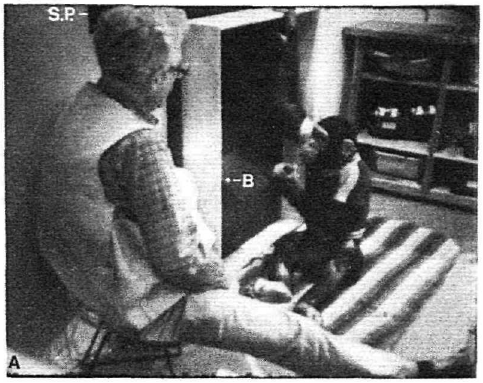
\includegraphics[width=103.65pt,height=82.19pt]{Figures/RL/gardner.png}};
%Image [id:dp007594076672443273] 
\draw (149.8,78.83) node  {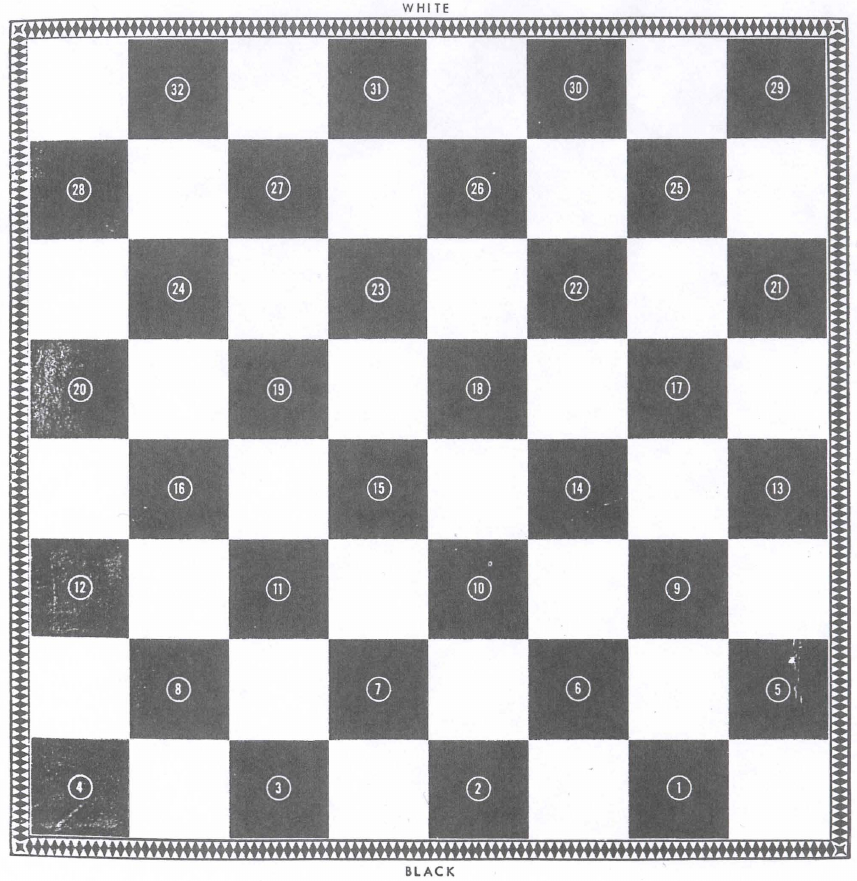
\includegraphics[width=66pt,height=67.85pt]{Figures/RL/checkerSamuel1959.png}};
%Image [id:dp3973383019437343] 
\draw (403.5,102.62) node  {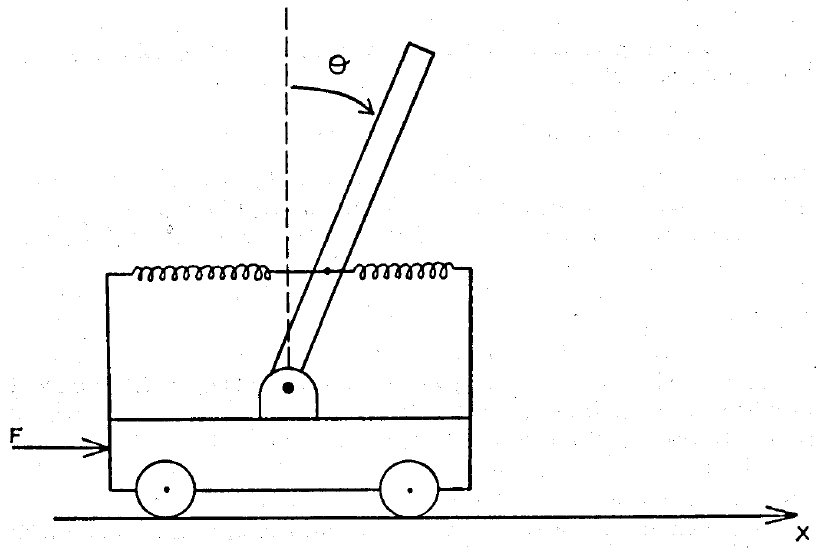
\includegraphics[width=107.25pt,height=72.03pt]{Figures/RL/Michie1968_cartpole.png}};
%Image [id:dp9659625193433798] 
\draw (403.9,257.9) node  {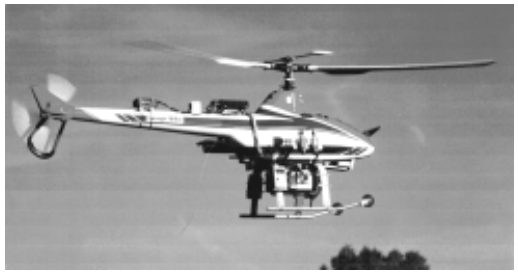
\includegraphics[width=110.25pt,height=63.15pt]{Figures/RL/Bagnell2001-helicopter.png}};
%Image [id:dp976485386281107] 
\draw (400.9,421.92) node  {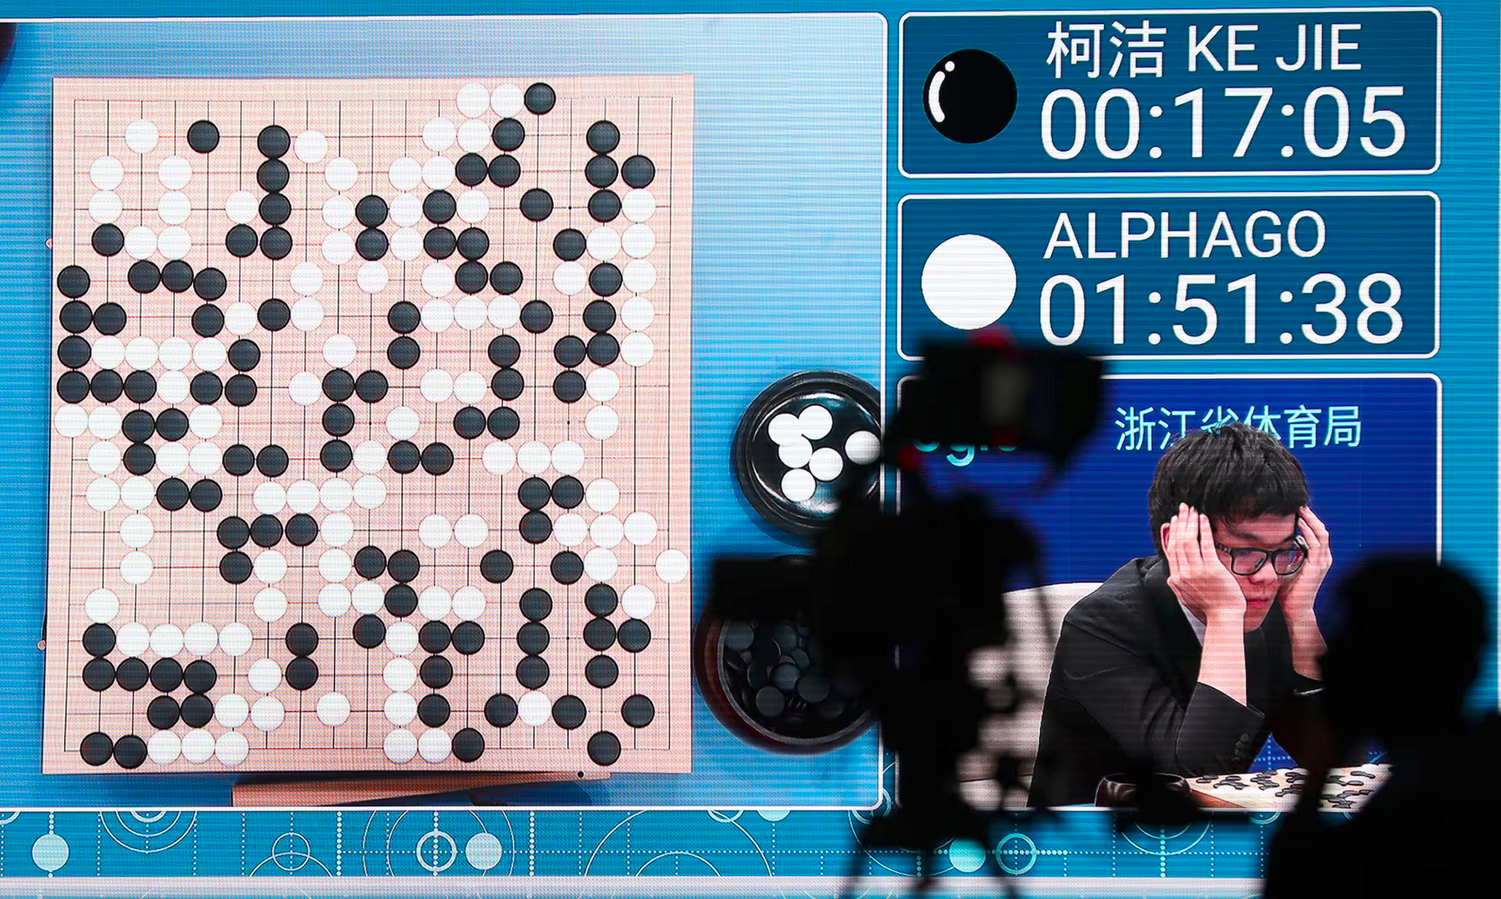
\includegraphics[width=136.05pt,height=81.48pt]{Figures/RL/alphago.png}};
%Image [id:dp6608675188149606] 
\draw (150.5,400.5) node  {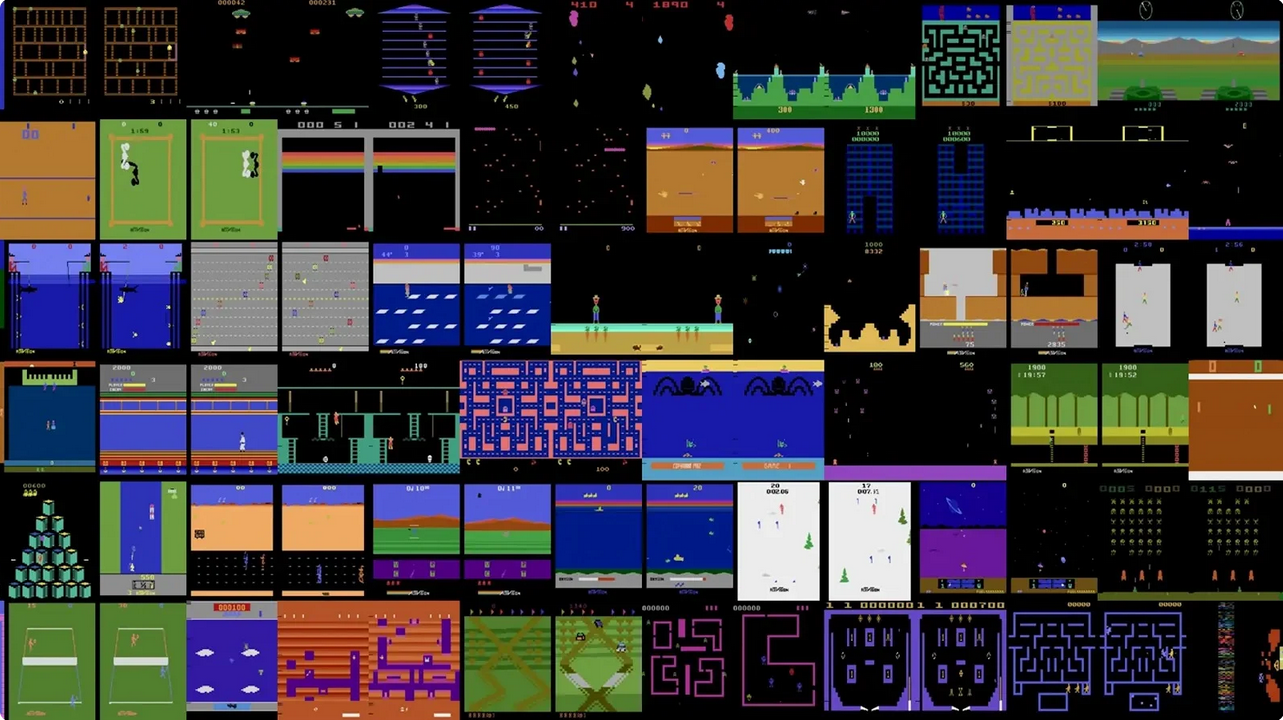
\includegraphics[width=96.45pt,height=87.45pt]{Figures/RL/atari.png}};
%Image [id:dp6327629891315109] 
\draw (149.8,570.8) node  {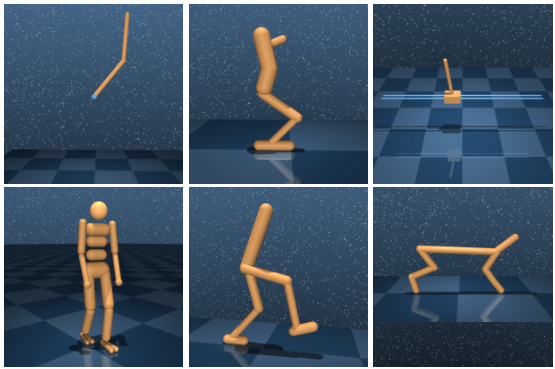
\includegraphics[width=140.7pt,height=91.2pt]{Figures/RL/deepmindcontrolsuite.png}};
%Image [id:dp4430575766949546] 
\draw (397,672.9) node  {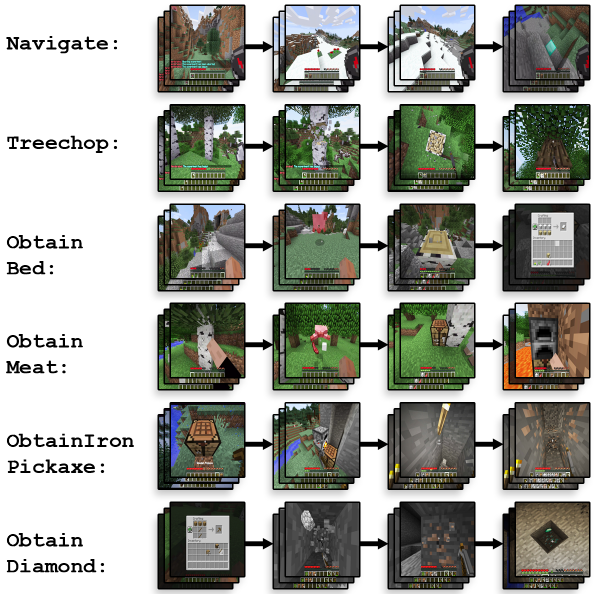
\includegraphics[width=156pt,height=159.15pt]{Figures/RL/minecraft-tasks.png}};
%Image [id:dp21646972126438868] 
\draw (150.7,755.97) node  {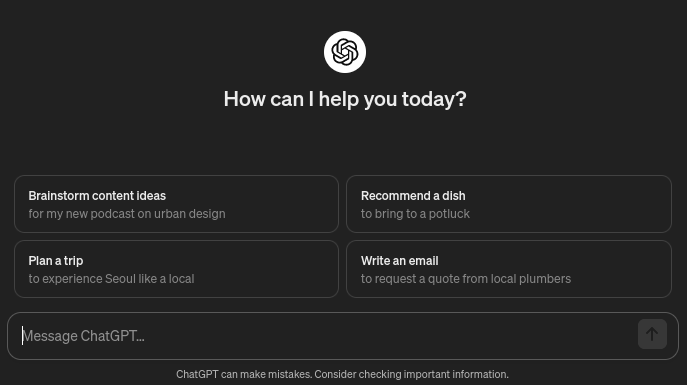
\includegraphics[width=159.45pt,height=89.36pt]{Figures/RL/chatgpt.png}};

% Text Node
\draw (55,291.2) node [anchor=north west][inner sep=0.75pt]  [font=\footnotesize] [align=left] {\begin{minipage}[lt]{140.34pt}\setlength\topsep{0pt}
\begin{center}
{\footnotesize (c) Teaching word to a chimpazee\\ \citep{Gardner1984_Chimpanzee}}
\end{center}
\end{minipage}};
% Text Node
\draw (67.6,126.8) node [anchor=north west][inner sep=0.75pt]  [font=\footnotesize] [align=left] {\begin{minipage}[lt]{114.1pt}\setlength\topsep{0pt}
\begin{center}
{\footnotesize (a) Checkers\\ \citep{Samuel1959_Checkers}}
\end{center}
\end{minipage}};
% Text Node
\draw (325.6,153.2) node [anchor=north west][inner sep=0.75pt]  [font=\footnotesize] [align=left] {\begin{minipage}[lt]{120pt}\setlength\topsep{0pt}
\begin{center}
{\footnotesize (b) Pole-balancing problem\\ \citep{Michie1968_Boxes}}
\end{center}
\end{minipage}};
% Text Node
\draw (316.8,303) node [anchor=north west][inner sep=0.75pt]  [font=\footnotesize] [align=left] {\begin{minipage}[lt]{125.74pt}\setlength\topsep{0pt}
\begin{center}
{\footnotesize (d) Flying an helicopter\\ \citep{Bagnell2001_Helicopter}}
\end{center}
\end{minipage}};
% Text Node
\draw (320.6,480.6) node [anchor=north west][inner sep=0.75pt]  [font=\footnotesize] [align=left] {\begin{minipage}[lt]{113.28pt}\setlength\topsep{0pt}
\begin{center}
{\footnotesize (f) AlphaGo vs. best human \\ \citep{Silver2016_AlphaGo}}\\{\scriptsize (Photograph by Wu Hong, in The Guardian)}
\end{center}
\end{minipage}};
% Text Node
\draw (74.8,464.2) node [anchor=north west][inner sep=0.75pt]  [font=\footnotesize] [align=left] {\begin{minipage}[lt]{106.35pt}\setlength\topsep{0pt}
\begin{center}
{\footnotesize (e) Atari benchmark\\ \citep{Bellemare2013_Atari}}
\end{center}
\end{minipage}};
% Text Node
\draw (32,636.8) node [anchor=north west][inner sep=0.75pt]  [font=\footnotesize] [align=left] {\begin{minipage}[lt]{170.5pt}\setlength\topsep{0pt}
\begin{center}
{\footnotesize (g) Deepmind Control Suite in MuJoCo\\ \citep{Tassa2018_DeepmindControl}}
\end{center}
\end{minipage}};
% Text Node
\draw (300,787.2) node [anchor=north west][inner sep=0.75pt]  [font=\footnotesize] [align=left] {\begin{minipage}[lt]{140.64pt}\setlength\topsep{0pt}
\begin{center}
{\footnotesize (h) Learning skills in Minecraft\\ \citep{Guss2019_MineRL}}
\end{center}
\end{minipage}};
% Text Node
\draw (61.2,823.2) node [anchor=north west][inner sep=0.75pt]  [font=\footnotesize] [align=left] {\begin{minipage}[lt]{123.08pt}\setlength\topsep{0pt}
\begin{center}
{\footnotesize (i) ChatGPT (chat.openai.com)\\ \citep{Ouyang2022_InstructGPT}}
\end{center}
\end{minipage}};
\end{tikzpicture}
\caption{Reinforcement learning environments in various domains of research.}
\label{fig:rl-envs}
\end{figure}

% RL in Robotics
Concurrently to games, RL has also been employed in optimal control and robotics. An early example of this is the classical pole-balancing problem~\citep{Michie1968_Boxes} that features a pole balancing on a moving cart (see Figure \hyperref[fig:rl-envs]{2.1.h}): the cart can move right or left and the reward is made only of a failure signal when the pole falls or the cart reaches the end of the track. While controlling robots is a major drive of RL research, it remains a great challenge. Robotics problems feature high-dimensional, continuous states and actions, which contrast with the discrete, finite states and actions of tabletop games. To overcome this, solutions include partitioning the space of states or actions to reduce complexity using linear function approximation~\citep{Busoniu2017_FuncApprox}, or using neural networks to learn to extract features from continuous states automatically~\citep{Bishop2006_Pattern} (see Section~\ref{sec:NN:DeepLearning}). Another attribute of robotic environments is partial observability, where robots only have incomplete information about the current state of the environment. This has been tackled by learning a model of the dynamics of the environment~\citep{Bagnell2001_Helicopter} (see Section \ref{sec:RL:Model-based}) or by providing the learner with memory to keep track of past information~\citep{Wierstra2007_POMDPs}. Another challenge is the design of a reward function. This requires translating the robot's objective into a numerical signal, which can be tedious. Intuitively, a robot could be rewarded positively when it completes its task. But this kind of sparse reward is difficult to learn. To fix this, reward shaping methods~\citep{Ng1999_Shaping, Laud2004_Shaping} construct rewards to consistently guide the learner towards the objective in a limited number of experiences. Finally, a last great challenge for learning robotic control with RL is the cost of experimenting with robots. Sample inefficiency and learning by trial-and-error make experimenting with physical hardware expensive and time-consuming. For these reasons, some approaches start by learning from demonstrations, before training with RL methods~\citep{Abbeel2006_Helicopter,Vecerik2017_Demonstrations}. Learning from demonstrated sequences of actions simplifies the learning problem by recasting it as a supervised learning problem. Another solution is to turn to simulated environments like ROS~\citep{Macenski2022_ROS} or MuJoCo (see Figure \hyperref[fig:rl-envs]{2.1.g}; \cite{Todorov2012_Mujoco}). However, using a model learnt in simulation in the real world is proven to be a difficult task because of the inevitable gap between the best simulations we have and the real world, a problem termed the "\textit{reality gap}" (see Section~\ref{sec:MAL:RealityGap} for more details on this issue). 
% To bridge this gap, many works have proposed ways to modify the simulated training phase by randomising the parameters of the simulation~\citep{Tobin2017_RealityGap, Chebotar2019_Sim2Real, Andrychowicz2020_Sim2Real} or by learning to efficiently adapt to a different environment~\citep{James2019_Sim2Real}. 
% Ajouter une phrase sur travaux récents qui utilisent rl among other things pour interagir avec des robots (peut-être parler de trucs hierarchiques, Levine2016EndtoEnd)

% RLHF
While control has been a main focus of RL, it has also been studied in other domains of artificial intelligence research. 
% A wide area of RL research has tackled problems in computational economics~\citep{Arthur1991_Economics,Charpentier2021_Economics}. 
A recent success has been the use of Reinforcement Learning from Human Feedback (RLHF;~\cite{Christiano2017_RLHF,Stiennon2020}) in language modelling. Language modelling is the task of learning to predict the next word in a given sequence. In this context, RLHF re-trains initially supervised language models to better fit human preferences. This technique is made possible by using reward modelling~\citep{Leike2018_RewardModel}, where a model learns to predict the rewards given by humans and is then used to train the RL model on a large number of experiences. This allowed the development of conversational agents like the now widely used ChatGPT~\citep{Ouyang2022_InstructGPT}. The success of RLHF approaches demonstrates the great potential of RL for learning to fit human needs. 

% Perspectives and limitations
All these examples show the tremendous potential of RL to shape artificial intelligence research further. This is largely due to the advent of deep reinforcement learning that sparked an ongoing revolution in the field during the last decade. Today, RL is widely considered an important block to building more advanced forms of artificial intelligence, if not the main tool to do so~\citep{Silver2021_RewardEnough}. However, this view is not shared by all~\citep{Mitchell2021_Harder} and RL still suffers from many limitations. We have already mentioned the problems of sample inefficiency, safety, and the high cost of RL training. They all generally hinder performance and prevent RL algorithms from being used extensively in robotics~\citep{Sunderhauf2018_Limits, Ibarz2021_Howto} and autonomous driving~\citep{Kiran2022_DRLDriving, Chen2023_EndToEndDriving}, with supervised alternatives like imitation learning being far superior~\citep{Hester2018_DQNfDemo}. These issues motivate various practical solutions~\citep{Ibarz2021_Howto}, like the aforementioned reward shaping strategy~\citep{Laud2004_Shaping}, as well as whole lines of research such as safe RL that explicitly constrain RL to learn from safe states~\citep{Garcia2015_SafeRL}, and curriculum learning that focuses on designing a schedule of increasingly difficult setups~\citep{Bengio2009_Curriculum, Uchendu2022_Jump}. RL also suffers from more practical issues inherent to its definitions and the tools it uses: reproducibility, high variance, and intricacy of the algorithms and their implementations~\citep{Hendersion2018_Matters}. Finally, as with the rest of methods based on deep neural networks, there is an issue of explainability and interpretability of deep RL. Deep neural networks act as black boxes that have no explicit mean for interpreting their reasoning and, thus, explaining their results~\citep{Rudin2019_StopExplain, Samek2021_ExplainDNN}. With deep RL agents, interpreting the learnt behaviours and understanding how training shaped them this way is often difficult. 
Some solutions are pursued, like hierarchical RL~\citep{Shu2018_Hierarchical, Pateria2021_HRLSurvey, Hafner2022_Hierarchical} or language-augmented RL (see Section \ref{sec:LAMAC:RW_LARL} for a more in-depth review of the literature on this matter).
% Parler de life-long learning/continual RL ?



% -------------------------------------------------------------------------


\section{Elements of Reinforcement Learning}\label{sec:RL:Elements}

\begin{figure}[h]
    \centering
    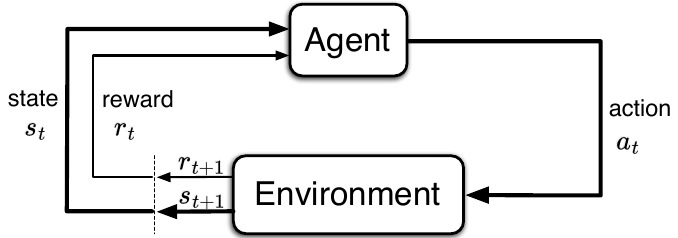
\includegraphics[width=0.8\textwidth]{Figures/RL/rl.jpg}
    \caption{Diagram of the reinforcement learning interaction between the agent and its environment, from \cite{Sutton2018_RL}.}
    \label{fig:rl}
\end{figure}

% Definition of main RL terms
Reinforcement learning is the process of learning how to complete a particular \textbf{task} from trial-and-error. In this process, we refer to the learner as an \textbf{agent}. The agent interacts with its \textbf{environment} over a sequence of discrete time steps denoted by $t=\{0,1,2,...\}$. Each interaction consists in the agent receiving information on its \textbf{state} $s_t$ from the environment and consequently choosing an \textbf{action} $a_t$ to perform. Following the agent's action, the environment produces a \textbf{reward} $r_{t+1}$ and a new state $s_{t+1}$. This process, illustrated in Figure \ref{fig:rl}, repeats indefinitely or stops after a finite number of steps $T$. In the latter case, we call this finite sequence of steps an \textbf{episode}. In the context of RL, the agent's goal is to pick the right actions to maximise the cumulative rewards in the long run. 

% Illustration of these terms
This terminology serves to describe any possible RL setting. The agent refers to the central entity of the experiment, defined concretely as a computer system. It is often considered "\textit{intelligent}" for being: (i) \textbf{reactive} to its environment, perceiving information from its surroundings and acting in response to these input signals; (ii) \textbf{proactive}, shaping its behaviour to satisfy its current goal; (iii) able to \textbf{learn} from its experience~\citep{Wooldridge1995_IntelligentAgents}. The goal of the agent is defined primarily by the task. It can be as straightforward as "picking up an object", or be a more abstract objective like "give this person what they need". The environment refers to the setting where this task is conducted, encompassing all elements except for the agent. The frontier between the agent and the environment is not a physical boundary but rather a conceptual one: everything that cannot be changed arbitrarily by the agent is considered part of the environment. For example, sensors, motors and mechanical joints of a robot should be considered as parts of the environment, while the agent in this case is the program controlling the robot. The states and actions depend on the agent's capabilities in the environment. Like the goal, they can take different forms, with various levels of abstraction. For example, the state of a robot could be concrete information about its surroundings coming from its sensors (e.g., camera, lidar, inertial measurement unit), or more symbolic information like the state of being in a particular room or not. Similarly, actions can be as concrete as "turning 4.5 degrees left", or more high-level like "flip the pancake". The RL framework accounts for all these levels of abstraction, allowing its use in many different settings. 




\subsection{Markov Decision Processes}\label{sec:RL:MDPs}

% States and actions
The universally accepted framework for building RL algorithms is the \textbf{Markov Decision Process} (MDP). The MDP is a mathematical formalisation of the RL problem. It defines this problem as a tuple $\langle\mathbf{S},\mathbf{A},\mathcal{T},\mathcal{R}\rangle$. In this tuple, $\mathbf{S}$ represents the set of all possible states in the environment: $\mathbf{S}=\{S_0,S_1,S_2,...\}$. Similarly, $\mathbf{A}$ is the set of all possible actions: $\mathbf{A}=\{A_0,A_1,A_2,...\}$. In the example of Figure \ref{fig:rl-toy}, $\mathbf{S}$ is the set of all eleven possible positions in the grid, numbered from 0 to 10, and $\mathbf{A}$ contains four possible actions: $\mathbf{A}=\{\mathtt{move\_up},\allowbreak\ \mathtt{move\_right},\allowbreak\ \mathtt{move\_down},\allowbreak\ \mathtt{move\_left}\}$. This setup describes the particular case of a \textit{finite} MDP, where the number of possible states and actions are finite. However, an MDP could also allow infinite states and actions if needed. For example, an autonomous driving system could have its state defined as a continuous GPS position and its action as the continuously defined rotation angle to apply to the steering wheel. 

% Transition probability
Next is the \textbf{transition function} $\mathcal{T}$ that defines the probability of transitioning from state $s$ to state $s'$ by taking action $a$:
\begin{equation}\label{eq:TransitionFunc}
    \mathcal{T}(s'\ |\ s,a)\coloneqq \text{Pr}\{s_{t+1}=s'\ |\ s_t=s,a_t=a\}.
\end{equation}
It dictates how the environment changes after performing an action. The transition function translates the robot's move in terms of probability: for example, in the setup of Figure \ref{fig:rl-toy}, $\mathcal{T}(S_1|S_0,\mathtt{move\_right})=1$ and $\mathcal{T}(S_4|S_0,\mathtt{move\_rigth})=0$. These probabilities describe a \textit{deterministic} environment, where a given action performed in a particular state always leads to the same outcome. On the other hand, in \textit{stochastic} environments, an action may have multiple possible outcomes. For example, an action may fail with a probability of 0.01: $\mathcal{T}(S_1|S_0,\mathtt{move\_rigth})=0.99$ and $\mathcal{T}(S_0|S_0,\mathtt{move\_rigth})=0.01$. In this synthetic environment, we control the probability of each transition. However, in more realistic settings, the transition function is unknown.

% Reward function
Finally, the \textbf{reward function} $\mathcal{R}$ is the expected value of the reward obtained during a transition from state $s$ to $s'$ with action $a$:
\begin{align}\label{eq:RewardFunc}
    \mathcal{R}(s,a)&\coloneqq\mathbb{E}[r_{t+1}\ |\ s_t=s,a_t=a]\notag\\
        &=\sum_{s'\in\mathbf{S}}\mathcal{T}(s'\ |\ s,a)r_{t+1}
\end{align}
In Figure \ref{fig:rl-toy}, the reward function is made of two elements: a positive reward signal if the agent reaches the goal and a negative signal for all other states. The former is straightforward: it indicates that the task is complete. The latter penalises the agent for entering any state that is not the terminal state. This kind of penalty is used often to urge the agent to complete the task as fast as possible: the more steps are taken, the larger the accumulated penalty. The reward depicted in Figure \ref{fig:rl-toy} can be described as \textit{sparse} because there are very few positive reward signals to guide the agent towards the objective. In this simple environment, this should not be an issue. But, in more complex settings with a larger number of possible states, sparse rewards can become problematic.

% Environment dynamics
Often, we see the transition probability and reward function brought together in a single function $p$ that defines the \textbf{environment dynamics}, with:
\begin{equation}
    p(s',r\ |\ s,a)\coloneqq \text{Pr}\{s_{t+1}=s',r_{t+1}=r\ |\ s_t=s,a_t=a\},
    \label{eq:EnvDyn}
\end{equation}
which is the probability of being in state $s'\in\mathbf{S}$ and receiving reward $r\in\mathbb{R}$, after performing action $a\in\mathbf{A}$ in state $s\in\mathbf{S}$.

% RL toy environment
\begin{figure}
    \centering
    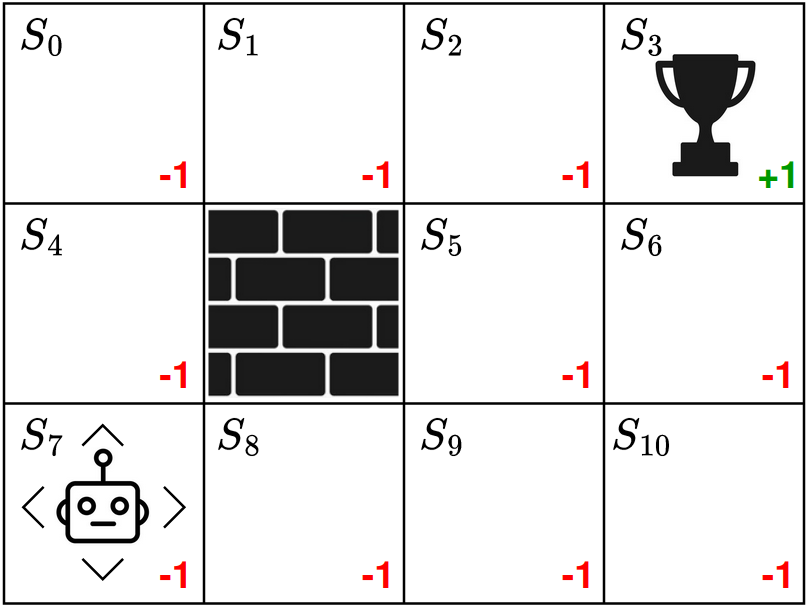
\includegraphics[width=0.5\textwidth]{Figures/RL/rl-toy.png}
    \caption{Simple reinforcement learning environment where the goal is for a robot to navigate in the grid and find the trophy cell. The robot can move in all four directions. The episode ends if the robot reaches the trophy or if the maximum number of steps $T$ is reached. States are defined by the position of the robot in the grid. Rewards for entering each state are indicated in the bottom-right corner of each cell.}
    \label{fig:rl-toy}
\end{figure}





\subsection{Modeling the Agent}\label{sec:RL:Agent}

% Policy
In the context of an MDP, the agent is modelled as a \textbf{policy} that selects actions depending on the current state of the environment. This policy can be either \textit{deterministic} or \textit{stochastic}. A deterministic policy is a function $\pi$ that directly maps the current state $s$ to an action $a$ to perform: $\pi:\mathbf{S}\rightarrow\mathbf{A}$, $\pi(s)=a$. A stochastic policy $\pi$ is defined as a function that maps states to probabilities over possible actions: the probability of choosing each action $a\in\mathbf{A}$ in state $s$ is $\pi(a|s)\in[0,1]$, with $\sum_{a\in\mathbf{A}}\pi(a|s)=1$. The policy function is used to describe how the agent selects its actions. In some algorithms, the policy is explicitly learnt during training. But, the policy might also be arbitrarily based on other learnt elements, or even random or unknown. 

% Trajectory and return
The agent uses the policy function to act in the environment, which results in a sequence of states, actions, and rewards that is called a \textbf{trajectory}, denoted $\tau$:
\begin{equation}
\tau=(s_0,a_0,r_1,s_1,a_1,r_2,s_2,a_2,...).
\end{equation}
The goal of an RL algorithm is to find a policy that maximises the accumulated rewards in the trajectories it generates. To that end, the policy must choose actions to maximise the sum of future rewards which is called the \textbf{return} $G_t$, starting from any step $t$:
\begin{equation}
G_t\coloneqq r_{t+1}+r_{t+2}+r_{t+3}+...+r_T,
\end{equation}
with the episode ending at step $T$. In the case where $T$ is infinite (i.e., the episode never ends) this formulation is problematic as it can result in an infinite return. This motivates another formulation of the return where future rewards are discounted by their distance in time to the current step. This \textbf{discounted return} is defined as:
\begin{equation}\label{eq:return}
    G_t\coloneqq r_{t+1}+\gamma r_{t+2}+\gamma^2 r_{t+3}+...=\sum_{k=0}^{\infty}\gamma^k r_{t+k+1},
\end{equation}
with $\gamma\in[0,1]$ the \textit{discount factor}. The discounted return favours rewards that are closer in time. The value of the discount factor controls how far in time the reward should affect the decision of the agent: a $\gamma$ close to zero will favour immediate rewards, while a $\gamma$ close to one will give importance to long-term returns. In practice, almost all RL methods use the discounted return, even if the episode ends in a finite number of steps $T$. 

% Value function
As the return cannot be computed before the end of the episode, many RL algorithms learn \textbf{value functions} to predict the expected return at any point during the episode. Thus, the \textbf{state-value function} associated with policy $\pi$, is defined as the expected return starting from any state $s$ and following policy $\pi$:
\begin{equation}
    V_\pi(s)\coloneqq\mathbb{E}_\pi[G_t\ |\ s_t=s],
    \label{eq:Value-def}
\end{equation}
where $\mathbb{E}_\pi[.]$ is the expected value of any random variable given that the agent always follows the policy $\pi$. Following the value of a particular state, we can also learn the value of performing a particular action in a particular state. This is the \textbf{action-value function} of policy $\pi$, defined as the expected return starting from state $s$, performing action $a$, and then following policy $\pi$:
\begin{equation}
    Q_\pi(s,a)\coloneqq\mathbb{E}_\pi[G_t\ |\ s_t=s,a_t=a].
    \label{eq:Qvalue-def}
\end{equation}
As we will see in further sections, these value functions can be learnt from experience and then used to choose actions accordingly or to do planning over multiple time steps. 

% Successiveness
An important property of the discounted return defined in Equation~\ref{eq:return} is its successiveness: the return at step $t$ can be expressed in function of the return of the following steps:
\begin{align}
    G_t&\coloneqq r_{t+1}+\gamma r_{t+2}+\gamma^2 r_{t+3}+\gamma^3 r_{t+4}+...\notag\\
       &=r_{t+1}+\gamma(r_{t+2}+\gamma r_{t+3}+\gamma^2r_{t+4}+...\notag\\
       &=r_{t+1}+\gamma G_{t+1}.
\end{align}
The same property can therefore be found for the state-value function:
\begin{align}
    V_\pi(s)&\coloneqq\mathbb{E}_\pi[G_t\ |\ s_t=s]\notag\\
       &=\mathbb{E}_\pi[r_{t+1}+\gamma G_{t+1}\ |\ s_t=s]\notag\\
       &=\mathbb{E}_\pi[r_{t+1}+\gamma V_\pi(s')\ |\ s_t=s,s_{t+1}=s'].
\end{align}

% Optimality
The \textit{optimal policy} is defined as the policy whose expected return is greater than or equal to that of all other possible policies, for all possible states. In other words, a policy $\pi$ is the optimal policy if $V_\pi(s)\geq V_{\pi'}(s)$, for all $s\in\mathbf{S}$ and all possible other policies $\pi'$. The optimal policy, denoted $\pi^*$ is associated with the optimal value functions $V^*$ and $Q^*$. By definition, the optimal policy always chooses the action with the largest action-value. That is,
\begin{equation}
    \pi^*(s)=\argmax_{a\in\mathbf{A}}Q^*(s,a).
\end{equation}
Following this, the optimal state-value function of any state $s$ is equal to the maximum value of $Q^*$ in this state:
\begin{align}
    V^*(s)&=\max_{a\in\mathbf{A}}Q^*(s,a)\notag\\
          &=\max_{a\in\mathbf{A}}\mathbb{E}_{\pi^*}[G_t\ |\ s_t=s,a_t=a]\notag\\
          &=\max_{a\in\mathbf{A}}\mathbb{E}_{\pi^*}[r_{t+1}+\gamma V^*(s')\ |\ s_t=s,a_t=a,s_{t+1}=s'].\label{eq:Bellman-v-exp}
\end{align}
This last result is the \textit{Bellman optimality equation}~\citep{Bellman1957_MDP} for the state-value function. By unfolding the expected value, we get:
\begin{equation}
    V^*(s)=\max_{a\in\mathbf{A}}\sum_{s'\in\mathbf{S}}\mathcal{T}(s'\ |\ s,a)\left[\mathcal{R}(s,a,s')+\gamma V^*(s')\right]. 
    \label{eq:Bellman-v}
\end{equation}
This is another form the Bellman optimality equation that will be used to define RL algorithms in the next section. It can also be expressed for the optimal action-value function as:
\begin{align}
    Q^*(s)&=\mathbb{E}_{\pi^*}[r_{t+1}+\gamma\max_{a'\in\mathbf{A}}Q^*(s_{t+1},a')\ |\ s_t=s,a_t=a]\notag\\
          &=\sum_{s'\in\mathbf{S}}\mathcal{T}(s'\ |\ s,a)\left[\mathcal{R}(s,a,s')+\gamma\max_{a'\in\mathbf{A}}Q^*(s',a')\right]. \label{eq:Bellman-q}
\end{align}
Bellman optimality equations are the basis of most RL algorithms, as they allow to gradually learn the optimal value functions through an iterative process described in Section~\ref{sec:RL:ValueIter}. In finite MDPs, the optimal value functions are proven to exist and be unique. But, that is not the case for more complex environments. Therefore, RL algorithms usually learn to estimate these functions through various techniques. 
%However, in environments with many possible states, this can require tremendous amounts of computational power and memory. The challenge becomes even more apparent in the case of an MDP with a continuous state space, i.e., a infinite number of different states. Thus, the algorithms presented in the next sections are used not necessarily to find the exact optimal behaviour, but rather to approximate the best way possible. Different approaches are developed to make these approximations better and, importantly, to reduce the computational power needed to learn fine policies for the agent. 

% Models
Finally, another tool used in RL is a \textbf{model} of the environment. A model predicts the outcomes of the agent's action in terms of changes in the environment and resulting rewards. Concretely, a model learns to approximate the environment dynamics $p$ defined in Equation~\ref{eq:EnvDyn}. Thus, the model is a function $\widehat{p}$ that maps the current state and action to the next state and reward. It can output a direct prediction, with $\widehat{p}:S\times A\rightarrow S\times\mathbb{R}$, or a probability distribution over states and rewards (like in Equation~\ref{eq:EnvDyn}).
%Similarly to the policy function, it can take two forms depending on the nature of its output. A \textit{distribution model} outputs a probability distribution over all states and rewards, like in Equation (\ref{eq:EnvDyn}). A \textit{sample model} outputs one possible transition based on the current state and action: $\widehat{p}:S\times A\rightarrow S\times\mathbb{R}$. Note that, given a distribution model, we can easily derive a sample model by sampling from the distribution. 
These two forms of models can be used in different ways for doing \textit{planning} over one or multiple time steps. As we will see in Section \ref{sec:RL:Model-based}, planning usually involves looking ahead by predicting future outcomes and then using these predictions to compute or improve value function predictions, which, in turn, can be used to select actions that maximise the expected return. 



% -------------------------------------------------------------------------



\section{Foundational RL Algorithms}\label{sec:RL:Algorithms}

After introducing the core elements used in RL, we present different approaches to learning from reinforcement. These approaches rely on learning value functions, policies, models, or a combination of the three, to devise an efficient strategy of actions. In this section, we present the foundational RL algorithms that serve as a basis for building deep RL and multi-agent RL methods. 


\subsection{Value Estimation}\label{sec:RL:Value-based}

% Introduction
As presented in the last section, value functions are a fundamental component of RL as they aim to predict the most important thing for the agent: the expected return of its actions. In RL algorithms, value functions are used for two different purposes:
\begin{itemize}
    \item First, to evaluate a given policy, which may be unknown, by estimating the expected return obtained following this policy. 
    \item Second, to explicitly learn a strategy to control the agent, in which case the agent's policy will be derived from the learnt value function. 
\end{itemize}
In both cases, the algorithms presented learn estimates of the value functions defined in the last section (see Equations~\ref{eq:Value-def} and~\ref{eq:Qvalue-def}). 


\subsubsection{Value Iteration}\label{sec:RL:ValueIter}

% Value iteration
To learn a value function estimate, a basic technique is \textit{value iteration}. It learns through an iterative process of gathering experience and improving the value function. Value iteration turns the Bellman optimality equations (see Equations \ref{eq:Bellman-v} and \ref{eq:Bellman-q}) into an update rule. That is, given a value function $V$ at our disposal, we compute a new value function based on the result of the Bellman equation:
\begin{equation}
    V(s)\leftarrow\max_{a\in\mathbf{A}}\sum_{s'\in\mathbf{S}}\mathcal{T}(s'\ |\ s,a)\left[\mathcal{R}(s,a,s')+\gamma V(s')\right],
    \label{eq:Value-iter}
\end{equation}
for each state $s\in\mathbf{S}$. The arrow indicates that we replace the current value $V(s)$, typically stored in a table with one value for each state, with a new one resulting from the calculation. In finite MDPs, executing this one time yields a new value function that is necessarily closer to the optimal value function. Thus, starting with an arbitrary initial value function (e.g., $V(s)=0$ for all $s\in\mathbf{S}$), repeating the value iteration operation ensures that $V$ converges towards $V^*$. In Figure \ref{fig:value-iter}, value iteration is executed on the simple RL environment previously introduced. This example shows how value iteration can learn the optimal value function quickly in a simple environment with a limited number of states. 

% Bootstrapping
An interesting property of such algorithms is the fact that they use the current estimate to compute the new one. This is called \textit{bootstrapping}. As we will see, this feature is at the core of many value estimation methods. Bootstrapping can greatly improve the convergence speed of these algorithms: in Figure \ref{fig:value-iter}, using the current estimate $V$ allows each iteration to have more impact (depending on the order in which states are processed). But, this can also induce difficulties: in more complex settings, using imperfect estimates can sometimes produce even worse new estimates, thus compromising the learning process. 

% Illustration of Value iteration
\begin{figure}
    \centering
    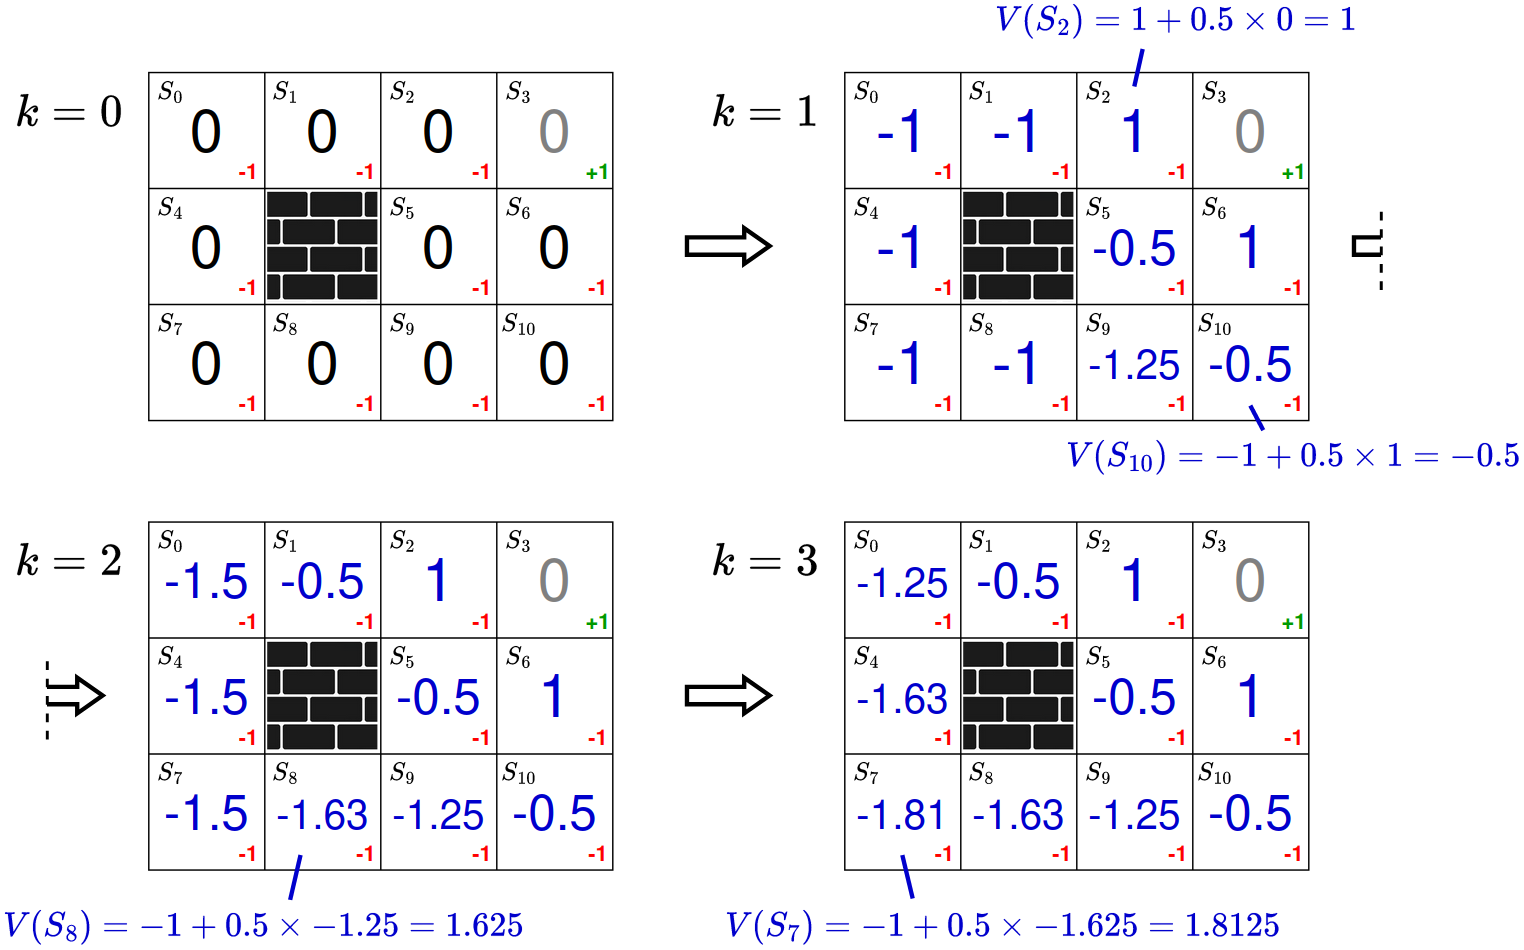
\includegraphics[width=1\linewidth]{Figures/RL/value-iter.png}
    \caption{Value iteration algorithm executed on the example of Figure \ref{fig:rl-toy}. We start with an initial value function $V(s)=0$ for all $s\in\mathbf{S}$. Then, each iteration $k$ applies the update rule of Equation~\ref{eq:Value-iter}, with $\gamma=0.5$, with the result $V(S_t)$ shown in the corresponding cell. As state $S_3$ is terminal, its value is considered to be 0. In three iterations, we converge to the optimal value function. Note that, because we compute the new $V$ for each state successively, the order of the states affects the result of each iteration and the number of iterations required for converging.}
    \label{fig:value-iter}
\end{figure}

\subsubsection{Monte Carlo Methods}\label{sec:RL:MonteCarlo}

% Monte-Carlo
A crucial drawback of the value iteration algorithm is that it assumes complete knowledge of the environment dynamics. Only because we know the probabilities of all transitions and their resulting reward, are we able to compute the expected value in the update rule (\ref{eq:Value-iter}). In most RL settings, the environment dynamics are unknown. Therefore, it is impossible to compute the exact value iteration update rule. What is often possible, however, is to run simulated experiments and gather sequences of states, actions and rewards. This is called "\textit{sampling}" trajectories from the environment. These sampled trajectories can then be used to compute approximations of what we want to predict. For example, given a trajectory $\tau$ generated using the sampling policy $\pi$, we can compute the return from any state $s\in\tau$ (according to Equation~\ref{eq:return}) and use the result as an estimation of the expected return from state $s$, i.e., $V_\pi(s)$. This is the core idea behind \textbf{Monte Carlo} methods: estimating the value function of a given policy by averaging sampled returns. This can be performed iteratively, by keeping a running estimate of the value function and updating it after each episode with:
\begin{equation}
    V_\pi(s_t)\leftarrow V_\pi(s_t)+\alpha\left[G_t-V_\pi(s_t)\right],
    \label{eq:Monte-Carlo}
\end{equation}
for all $t<T$, with $G_t$ the experienced return from state $s_t$ and $\alpha\in]0,1]$ a constant parameter called the \textbf{learning rate}. This update modifies the value of $V_\pi(s_t)$ by "moving it" towards the experienced return. The learning rate $\alpha$ controls the magnitude of this modification: $\alpha=1$ would mean the new value of $V_\pi(s_t)$ is $G_t$, $\alpha<1$ yields a new value between the old $V_\pi(s_t)$ and $G_t$. Using a learning rate is important because one sampled return is a poor approximation of the actual state-value function. Thus, repeating this update many times will allow to gradually move towards a better estimate of $V_\pi(s_t)$.

\subsubsection{Temporal Difference Learning}\label{sec:RL:TD}

% TD
A problem with Monte Carlo methods is that they require waiting for the end of each episode to compute the return of all states. In some environments, the episode might last for several hours or even never end, making Monte Carlo methods impractical. A solution for this is to use \textbf{Temporal-Difference} (TD) learning~\citep{Sutton1988_TD}. TD methods similarly learn an estimate of the value function, but using only a limited number of transitions. The simplest TD method, called \textit{TD(0)}, updates the value after only one time step, with
\begin{equation}
    V_\pi(s_t)\leftarrow V_\pi(s_t)+\alpha\left[r_{t+1}+\gamma V_\pi(s_{t+1})-V(s_t)\right].
    \label{eq:TD}
\end{equation}
The return in the Monte Carlo update rule (Equation~\ref{eq:Monte-Carlo}) is replaced by its estimation using the current value function. The expression inside the brackets is often referred to as the \textit{TD-error} or \textit{Bellman error} as it is derived from the Bellman equation (\ref{eq:Bellman-v}). It measures the difference between the current estimated value of $s$ and the better estimate $r_{t+1}+\gamma V_\pi(s_{t+1})$ given by TD(0), called the \textit{TD-target}. The TD-target, can be extended to use the experience of multiple time steps to have a better estimate of the return~\citep{Sutton1988_TD}. 
%However, the one-step version is often preferred for its simplicity. 

% SARSA
% For now, we have shown how to find the value function associated to a given policy that produces trajectories. We will show in the next sections how this can help learning better policy functions. But, with only a value function, TD applied to the action-value function can learn an effective policy to control the agent. Similarly to Equation~\ref{eq:TD}):
% \begin{equation}
%     Q(s_t,a_t)\leftarrow Q(s_t,a_t)+\alpha\left[r_{t+1}+\gamma Q(s_{t+1},a_{t+1})-Q(s_t,a_t)\right].
%     \label{eq:SARSA}
% \end{equation}
% This update rule uses the tuple $\langle s_t,a_t,r_{t+1},s_{t+1},a_{t+1}\rangle$ to update the current estimate of $Q$. This tuple gave its name the to the algorithm \textit{SARSA}~\citep{} that uses this update rule to learn a better action-value function and use it for control. To do so, the agent simply chooses the action with the highest action-value. After each transition, the action-value function can be updated using the experience of the last two steps. 

\subsubsection{Q-Learning}\label{sec:RL:Qlearning}

% Q-learning
For now, we have looked at methods to learn estimates of the state-value function. The \textit{Q-learning} algorithm~\citep{Watkins1989_RL} applies TD learning to the action-value function to directly learn an efficient way to control the agent. Given many transition tuples of form $\langle s_t,a_t,r_{t+1},s_{t+1}\rangle$, we can learn an action-value function $Q$ with:
\begin{equation}
    Q_\pi(s_t,a_t)\leftarrow Q_\pi(s_t,a_t)+\alpha\left[r_{t+1}+\gamma\max_aQ_\pi(s_{t+1},a)-Q_\pi(s_t,a_t)\right].
    \label{eq:Qlearning}
\end{equation}
This update rule uses the current estimate $Q$ as an approximation of the optimal $Q^*$ to compute the Bellman error. With this update, Q-learning learns the action-value function of the "\textit{greedy} policy with respect to $Q$", i.e., the policy that always chooses the action with the highest action-value according to Q: $\pi(s)=\argmax_aQ_\pi(s,a)$. Given enough training, the learnt action-value function can be used to choose actions following the greedy policy. 

% Exploration-Exploitation
This method is shown to effectively learn a good approximation of $Q^*$ as long as all states are explored enough. Thus, it requires a sampling policy to explore the environment and gather the transition tuples. The simplest possible policy is to randomly select actions in all steps. But, this means that some irrelevant states will be explored as much as others. Instead, we might want to focus on the states and actions that have more potential. This is a common dilemma in RL algorithms, where we need to balance a trade-off between \textit{exploration} and \textit{exploitation}:
\begin{itemize}
    \item We want to explore different behaviours to better understand the environment dynamics and improve our estimations. 
    \item But, at the same time, we want to exploit our past findings to learn faster.
\end{itemize}
In the case of Q-learning, exploration is done by randomly selecting actions. And, exploitation is done by using the greedy policy to select action.  

% Epsilon-greedy
To balance the exploration-exploitation trade-off, Q-learning employs the $\epsilon$\textit{-greedy} policy. At each time step, $\epsilon$-greedy decides between choosing an action randomly or following the greedy policy. It uses a parameter $\epsilon$ between 0 and 1 that determines the probability of choosing the action randomly. Typically, this parameter starts at 1 and decreases throughout training towards 0. This allows a progressive shift between random exploration at the start when the estimations are bad, and exploitation when estimations start getting better. While this is far from being a perfect exploration strategy (more on that in Chapter \ref{ChapterJIM}), it offers a simple solution for exploration in Q-learning. An algorithm for executing Q-learning with $\epsilon$-greedy is described here: 
\begin{algorithm}
\caption{Q-learning with $\epsilon$-greedy policy}
\label{alg:q_learning}
\begin{algorithmic}
\State Initialize $Q(s, a)$ arbitrarily
\State Initialize $\epsilon=1$
\State Initialize $\alpha$ (learning rate), $\gamma$ (discount factor)
\For{each episode}
    \State Initialize state $s_0$
    \For{t=0,...,T}
        \State Execute $\epsilon$-greedy policy:\\
        \hspace{45pt} With probability $\epsilon$, choose a random action $a_t$\\
        \hspace{45pt} Otherwise, choose $a_t = \argmax_a Q(s_t, a)$
        \State Perform action $a_t$, observe reward $r_{t+1}$ and new state $s_{t+1}$
        \State $Q(s_t, a_t) \gets Q(s_t, a_t) + \alpha \left[r_{t+1}+\gamma\max_{a}Q(s_{t+1},a)-Q(s_t,a_t) \right]$
        \State $s_t\gets s_{t+1}$
        \State $\epsilon\gets\text{max}(\epsilon-0.001,0)$
    \EndFor
\EndFor
\end{algorithmic}
\end{algorithm}

% Tabular
An important observation to make about all value-based methods presented in this section is the fact that they all rely on a list of values to keep track of the current estimations. In Q-learning, for example, the action-value function is represented as a table with states as rows and actions as columns, where each cell $(s,a)$ contains the current estimate $Q(s,a)$. For this reason, these approaches are qualified as "tabular". This aspect highlights a clear drawback of these methods: they are limited in the number of single values they can keep track of. To learn a perfect policy or value function, we would need to exhaustively try all possible actions in all possible states. But, this is impossible in rich environments with very large, if not continuous, state and action spaces. Thus, tabular value functions are limited to environments where they can realistically explore all states or state-action pairs enough times to build good value estimates. In fact, they are even incapable of dealing with continuous states and actions, as they would require infinitely large value tables, which makes their application to real world tasks significantly more difficult.

% Parameterised value
A solution for this is to change the form of the value function and represent it as a parameterised function. Instead of keeping track of all values in a table, the value function is defined as a mathematical function of states that outputs the value of the input state. We would write the value functions as $V(s,\varphi):S\times\mathbb{R}^{d^\varphi}\rightarrow\mathbb{R}$ or $Q(s,a,\varphi):S\times A\times\mathbb{R}^{d^\varphi}\rightarrow\mathbb{R}$, with $\varphi\in\mathbb{R}^{d^\varphi}$ a vector of parameters of dimension $d^\varphi$ used to define the value function. The actual definition of the function is arbitrary. It can be as simple as a linear transformation of the input state, or use more complex definitions such as artificial neural networks (see Section \ref{sec:NNs}). In any case, $\varphi$ is the set of real-valued parameters that dictates the outputs of the value function. An advantage of having a parameterised value function is that it can now deal with continuous states. There is no more table keeping track of all possible values. The new value function should now be able to predict the value of states it has never seen before, by generalising from its training experience (see Section~\ref{eq:DQN} for more detail). But, this also comes with downsides. Learning a set of parameters that generalises well can be difficult. From the designer's point of view, the value function is now a black box that computes values from a series of mathematical operations, which can be hard to interpret. 

% Conclusion
Despite their limitations, value-based approaches are still widely used across RL research. Their simple definition and low computational resources make them easy to implement. In the next sections, we will describe ways to alleviate some of the drawbacks of value-based algorithms. Furthermore, we will see that, when combined with other techniques, value functions play a crucial role in building good RL agents. 

\subsubsection{On-Policy vs. Off-Policy Learning}\label{sec:RL:On/Off-policy}

% On- vs Off-policy (SARSA)
Q-learning, as defined in Algorithm \ref{alg:q_learning}, is characterised as an \textbf{off-policy} algorithm, because its update does not depend on the policy used to generate the experience, which is referred to as the \textit{behaviour} policy. This is in contrast with \textbf{on-policy} algorithms, such as SARSA~\citep{Rummery1994_SARSA}, that learns an action-value function, similarly to Q-learning, but based on an experience tuple $\langle s_t,a_t,r_{t+1},s_{t+1},\\a_{t+1}\rangle$:
\begin{equation}
    Q(s_t,a_t)\leftarrow Q(s_t,a_t)+\alpha\left[r_{t+1}+\gamma Q(s_{t+1},a_{t+1})-Q(s_t,a_t)\right].
    \label{eq:SARSA}
\end{equation}
The difference with the Q-learning update (see Equation~\ref{eq:Qlearning}) is in the choice for action at state $s_{t+1}$, used in the TD-target:
\begin{itemize}
    \item SARSA uses the action $a_{t+1}$ that was selected by the behaviour policy. Therefore, its update depends on the current behaviour policy of the agent (i.e., on-policy).
    \item Q-learning uses the learnt action-value to select a greedy action that serves as $a_{t+1}$ in the TD-target: $r_{t+1}+\gamma\max_{a}Q(s_{t+1},a)$. This TD-target depends only on $Q$ and is independent of the behaviour policy (in this case the $\epsilon$-greedy policy). Thus, Q-learning is off-policy. 
\end{itemize}
In other words, off-policy value learning learns the value of a policy (in this case, the greedy policy with respect to $Q$), using another policy to gather experiences (here, $\epsilon$-greedy). On the other hand, on-policy value learning directly learns the value of the behaviour policy. Note that, while we illustrate these properties with action-value learning algorithms, these can be used to characterise state-value or policy learning algorithms (see Sections \ref{sec:RL:Policy-based} and \ref{sec:DRL:Policy}).

% Experience Replay
The distinction between on- and off-policy is subtle but has one major implication. Off-policy algorithms can learn functions (value or policy) based on data generated by other, totally separate processes. For example, Q-learning could learn the optimal action-value function based on experiences gathered by a random policy, a pool of various independent policies, or even human experts. This particular feature allows using \textbf{experience replay}~\citep{Lin1992_ExperienceReplay}, where, during training, experiences are stored in a memory, called the \textit{replay buffer}, and are then reused any number of times in later updates. To make an update, a batch of past experiences is drawn randomly from the replay buffer and the learning update is performed on all these samples. Training on past experiences allows learning on more diverse data, thus specialising less on the current behaviour policy. In this case, off-policy learning is required because the replay buffer is full of past experiences generated by previous (different because trained fewer times) versions of the behaviour policy. 






\subsection{Policy Gradients}\label{sec:RL:Policy-based}

\subsubsection{Learning a Parameterised Policy Function}

% Learning a parameterised policy
In Section \ref{sec:RL:Agent}, we said that an RL agent is primarily defined by its policy function $\pi$, which maps states to actions. We saw in the last section that value functions can be used to evaluate an unknown policy or even to learn a policy by being greedy with respect to an action-value function. Another possible approach is to directly learn the policy function. This can be done by representing the policy function as a parameterised mathematical function of states which outputs either a probability over possible actions, in the case of a stochastic policy, or directly the action to perform, for a deterministic policy. For these two possible cases, we write:
\begin{equation}
    \pi(a\ |\ s,\theta)=Pr\{a_t=a\ |\ s_t=s,\theta_t=\theta\},
\end{equation}
or
\begin{equation}
    \pi(s;\theta)=a,
\end{equation}
where $\theta\in\mathbb{R}^{d^\theta}$ is the set of learnt parameters of the policy function. We also denote such policy $\pi_{\theta}$, as the policy defined by parameters $\theta$. 

% Gradient ascent
To maximise future rewards, we have to find the set of values for $\theta$ that produces the best sequences of actions. To do so, we can sample experiences from the environment and accordingly modify $\theta$ to improve the policy. This can be done using \textbf{gradient ascent}, which gradually modifies the parameters to maximise a given measure of performance $J(\theta)$:
\begin{equation}
    \theta_{t+1}=\theta_t+\alpha\nabla J(\theta_t),
    \label{eq:GradientAscent}
\end{equation}
where $\alpha\in]0,1]$ is a small learning rate and $\nabla J(\theta_t)$ is the gradient of the objective $J(\theta_t)$ with regards to the policy parameters $\theta$ at time step $t$. It is a vector that shows in which direction in the parameter space to move $\theta$ to maximise the objective. Thus, Equation~\ref{eq:GradientAscent} replaces the current parameters $\theta_t$ with a new set of values $\theta_{t+1}$ that yields better values of $J$. 



\subsubsection{The Policy Gradient Theorem}\label{sec:Policy:PolicyGradientTheorem}

% Policy gradient theorem
In RL, the objective to maximise is the sum of future rewards. Thus, we can define the objective using the true value function of our policy: $J(\theta)=V_{\pi_{\theta}}(s_0)$, with $s_0$ being the initial state of the episode. Given this, for a discrete MDP and a given stochastic policy $\pi_{\theta}$, we can devise the \textbf{policy gradient theorem} that yields:
\begin{equation}
    \nabla J(\theta)=\sum_s\rho_{\pi_{\theta}}(s)\sum_aQ_{\pi_{\theta}}(s,a)\nabla\pi_\theta(a\ |\ s),
    \label{eq:PolicyGradient:Theorem}
\end{equation}
with $Q_{\pi_{\theta}}$ the true action-value function of policy $\pi_{\theta}$ and $\rho_{\pi_{\theta}}(s)$ the probability of experiencing state $s$ if we follow policy $\pi_{\theta}$. 
%The proof of this theorem is given in Annex \ref{app:RL:PolicyGradientTheorem}. 

% Reinforce
If policy $\pi_{\theta}$ is followed, then the theorem can be formulated with an expected value:
\begin{align}
    \nabla J(\theta)&=\mathbb{E}_{s\sim\rho_{\pi_{\theta}}}\left[\sum_aQ_{\pi_{\theta}}(s,a)\nabla\pi_\theta(a\ |\ s)\right]\label{eq:PolicyGradient:Exp}\\
    &=\mathbb{E}_{s\sim\rho_{\pi_{\theta}}}\left[\sum_a\pi_\theta(a\ |\ s)Q_{\pi_{\theta}}(s,a)\frac{\nabla\pi_\theta(a\ |\ s)}{\pi_\theta(a\ |\ s)}\right]\notag\\
    &=\mathbb{E}_{s\sim\rho_{\pi_{\theta}},a\sim\pi_{\theta}}\left[Q_{\pi_{\theta}}(s,a)\frac{\nabla\pi_\theta(a\ |\ s)}{\pi_\theta(a\ |\ s)}\right].\label{eq:PolicyGradient:sampleA}
\end{align}
The expected value in Equation~\ref{eq:PolicyGradient:Exp} is obtained by sampling $s\sim\rho_{\pi_{\theta}}$. Likewise, in Equation~\ref{eq:PolicyGradient:sampleA}, the sum is absorbed in the expectation by sampling $a\sim\pi_{\theta}$. Because $Q_{\pi_\theta}(s,a)=\mathbb{E}_\pi[G_{s,a}|s,a]$, by definition, we can rewrite the policy gradient as:
\begin{equation}
    \nabla J(\theta)=\mathbb{E}_{\pi_{\theta}}\left[G_{s,a}\frac{\nabla\pi_\theta(a\ |\ s)}{\pi_\theta(a\ |\ s)}\right].
    \label{eq:REINFORCE}
\end{equation}
This expectation can be approximated by sampling many trajectories. The algorithm REINFORCE~\citep{Williams1992_Reinforce} uses this to update the parameters $\theta$:
\begin{equation}
    \theta_{t+1}\leftarrow\theta_t+\alpha G_t\frac{\nabla\pi_\theta(a_t\ |\ s_t)}{\pi_\theta(a_t\ |\ s_t)},
\end{equation}
for any state $s_t$ and action $a_t$ from which the agent has experienced the return $G_t$. In this update, the gradient of the policy indicates the direction, in parameter space, that most increases the probability of choosing action $a_t$. By taking the product of this gradient with the return $G_t$, this update increases the probability of actions depending on the returns they generate. High positive returns will result in high increases in the corresponding actions, and conversely for negative returns. Then, dividing by the probability of the action ensures that actions that are selected more frequently are not over-estimated by getting more updates of the same magnitude. Therefore, the REINFORCE update conveniently increases the probability of choosing actions that yield good returns and decreases the probability of actions that yield bad ones. 

\subsubsection{The Actor-Critic Architecture}\label{sec:Policy:Actor-Critic}
% Actor-Critics
As it uses the complete return, REINFORCE is a Monte Carlo method for learning a parameterised policy function. Like the Monte Carlo approach presented in the last section, REINFORCE requires waiting for the end of the episode to update the policy. But, again, we can use the principle of TD learning (see Section \ref{sec:RL:TD}) to solve this issue, by replacing the return by its estimation with a value function:
\begin{equation}
    \theta_{t+1}\leftarrow\theta_t+\alpha\left(r_{t+1}+\gamma V(s_{t+1})\right)\frac{\nabla\pi_\theta(a_t\ |\ s_t)}{\pi_\theta(a_t\ |\ s_t)},
\end{equation}
or,
\begin{equation}
    \theta_{t+1}\leftarrow\theta_t+\alpha Q(s_t,a_t)\frac{\nabla\pi_\theta(a_t\ |\ s_t)}{\pi_\theta(a_t\ |\ s_t)},
\end{equation}
where $V$ and $Q$ would be learnt value functions that estimate the true value functions of the current policy $\pi$. This kind of approach is referred to as \textit{actor-critic} methods~\citep{Barto1983_ActorCritic, Sutton1984_ActorCritic}, where the policy is the actor who learns to select action, and the value function is the critic who evaluates the policy's actions. In this case, the value function is used only to guide the learning process of the policy. 
% Si besoin dans la suite: ajouter explication des baseline dans PG et A2C ici

% DPG
In the last section, we introduced parameterised value functions as a way to use value functions with continuous states. However, a parameterised version of Q-learning would still not be able to deal with continuous actions efficiently. That is because finding a greedy policy with respect to a continuous action-value function would be an optimisation problem in itself: finding the global maximum of a given function. But, thanks to an actor-critic architecture, a solution to this issue can be found. By extending the policy gradient theorem defined in Equation~\ref{eq:PolicyGradient:Exp} to continuous actions and a deterministic policy, we can find that
\begin{equation}
    \nabla J(\theta)=\mathbb{E}_{s\sim\rho_{\pi_\theta}}\left[\nabla_{\theta}\pi_\theta(s)\nabla_aQ_\varphi(s,a)\ |\ a=\pi_\theta(s)\right].
    \label{eq:DPG}
\end{equation}
This the \textbf{deterministic policy gradient theorem} (DPG), as defined by \cite{Silver2014_DPG}, which gives the following update for the parameters $\theta$:
\begin{equation}
    \theta_{t+1}\leftarrow\theta_t+\alpha_\theta\nabla_\theta\pi_\theta(s_t)\nabla_aQ_\varphi(s_t,a_t).
    \label{eq:DPG}
\end{equation}
The parameters of the action-value function $\varphi$ are updated as well to minimise the Bellman error:
\begin{align}
    \delta_t&=r_t+\gamma Q_\varphi(s_{t+1},a_{t+1})-Q_\varphi(s_t,a_t)\\
    \varphi_{t+1}&\leftarrow\varphi_t+\alpha_\varphi\delta_t\nabla_\varphi Q_\varphi(s_t,a_t).
\end{align}
Intuitively, DPG can be understood as an extension of Q-learning for continuous actions, where the $\epsilon$-greedy policy is replaced by a learnt policy trained to select the actions that maximise $Q_\varphi$. 

% ? Continuous actions (sampling actions)


% Conclusion: policy-based, why, other approaches derived from PG, complementary with values 
All RL approaches that derive from the policy gradient theorem are referred to as \textit{policy-based}, even the actor-critic that also learns value functions. A first appeal to policy-based methods is intuitive: it seems logical to explicitly learn to perform actions more often if they produce better returns, and conversely. The great advantage of policy-based methods, however, is in their capacity to handle continuous state and action spaces~\citep{Williams1992_Reinforce}. Parameterised value functions can deal with continuous states but, as we have seen, are still unable to handle continuous actions without being paired with a learnt policy or using discretisation methods. Thus, policy-based methods are a logical choice for more fine-grained control environments. That said, value-based still have their advantages. Depending on the setting, it might be simpler to learn a value function than a policy. In this sense, actor-critic algorithms offer a convenient integration of both. We will see in Section \ref{sec:DRL} that most state-of-the-art RL algorithms use this approach. 






\subsection{Planning with Models}\label{sec:RL:Model-based}

% Intro model-free/model-based
The two previous sections presented algorithms that learn a policy, a value, or both, and rely on the learnt elements to select actions in each step. These methods are often called \textbf{model-free} because they do not use a model of the environment dynamics. That is in contrast with \textbf{model-based} methods that rely primarily on a model to learn an efficient strategy, as defined in Section \ref{sec:RL:Elements}. Having a model that predicts future outcomes allows to simulate experiences and use these to devise a strategy. This may involve learning value and policy functions as well. The key difference with model-free techniques lies in the exploitation of a learnt model of the environment to improve the learning and usage of policy and value functions.

\subsubsection{Learning the Model}
% Intro
Learning the model is a supervised task where the agent learns to approximate the environment dynamics using its own experienced transitions as training examples. The goal is to learn a good approximation $\widehat{p}$ to use for planning. As $\widehat{p}$ learns two distinct elements, the transition probability $\mathcal{T}$ and the reward function $\mathcal{R}$, the prediction task is often separated in two as well, with $\widehat{\mathcal{T}}$ and $\widehat{\mathcal{R}}$. 

% Tabular
The simplest way to learn these functions is by learning a \textit{tabular model}~\citep{Sutton1991_Dyna}. In a discrete MDP, we can store the number of occurrences of all transitions $n(s,a,s')$ and use it to output a probability for each possible next state:
\begin{equation}
    \widehat{\mathcal{T}}(s'\ |\ s,a)=\frac{n(s,a,s')}{\sum_{s"\in\mathbf{S}}n(s,a,s")}.
\end{equation}
Similarly, for the reward, we can store the rewards obtained in each transition $r(s,a,s')$ and use them to approximate the expected reward of each transition by computing a mean over sampled transitions:
\begin{equation}
    \widehat{\mathcal{R}}(s,a,s')=\frac{1}{N}\sum_{k=0}^{N}r_k(s,a,s'),
\end{equation}
with $N=n(s,a,s')$. 
This tabular solution can be effective in small discrete MDPs. However, it does not scale well to environments with many possible transitions.

% Parametric
To tackle this issue, another approach is to define the model as a parametric function $\widehat{p}(s,a,\psi)$ with parameters $\psi\in\mathbb{R}^{d^\psi}$. Like for value and policy functions, this parameterised function can take many different forms. Parameterised models have been defined using various machine learning algorithms like linear regression~\citep{Sutton2008_DynaLinearReg}, random forest~\citep{Hester2012_TEXPLORE}, and neural networks~\citep{Narendra1990_NNSystemIdent, Oh2015_DeepModel}. 

\subsubsection{Using the Model}
% Learning-focused model
We introduced models as a tool to perform planning by simulating experience. Planning itself can serve different purposes. One approach is to use the model to learn better approximations of value and policy functions. Instead of gathering experiences in the environment, a model can be queried to simulate transitions. These simulated transitions can then be used for computing the learning objectives of any algorithm. For example, in Dyna~\citep{Sutton1991_Dyna}, a tabular model is used to perform many Q-learning updates between each environment step. This improves sample efficiency by increasing the number of updates for each call to the environment. Other learning algorithms require the environment dynamics to perform their update, like value iteration (see Section \ref{sec:RL:ValueIter}) or guided policy search~\citep{Levine2013_GPS}. In such cases, learning a model enables using these algorithms in complex environments with unknown dynamics~\citep{Abbeel2006_Helicopter,Levine2014_GPS-model}. 

% Decision-focused model (exhaustive/heuristic search, MCTS)
A second approach focuses the model on the decision part of the algorithm. In this sense, planning is used to predict many different paths of states and actions, and ultimately choose the path leading to the best return. This can be done in an exhaustive manner, by simulating all possible paths until the completion of the episode. Then, the value of each observed state can be computed as a mean of all returns obtained from this state~\citep{Tesauro1996_MonteCarloSearch}, similarly to Monte Carlo methods (see Section \ref{sec:RL:MonteCarlo}). Planning in this way is particularly effective, especially in environments where a perfect model is given like Chess or Go. But, it requires a great amount of computation to simulate all trajectories and evaluate each state and action. Doing an exhaustive search of all possible outcomes is unrealistic in environments with a large state space. In the game of Go, the number of possible states is beyond any computing limitation. To handle this, the Monte Carlo Tree Search algorithm (MCTS; \cite{Coulom2006_MCTS}) had to greatly optimise the search by parallelising the computation of different paths of actions, excluding states that are probably not good, and learning both an action-value and a policy function. Thanks to efficient planning, MCTS is the core algorithm responsible for a series of breakthroughs in playing board games, such as in the game Go considered very hard for its large count of possible board situations~\citep{Coulom2006_MCTS,Finnsson2008_GamePlaying,Silver2016_AlphaGo,Schrittwieser2019_Muzero}.

% Problems and avantages of planning (computation intensive / sample efficient, better generalisation (learns dynamics that true in all the environment, which very not true for values or policies))
Overall, model-based methods have many advantages. Intuitively, learning the environment dynamics seems logical, as the model learns general knowledge about the environment that should generalise well to all parts of the environment, which is not necessarily the case for value and policy functions. Model-based approaches are often more sample efficient than model-free ones. By using the model's prediction to train policies and values, they can require less experience in the real environment to come up with a good strategy. However, models still have their limitations. Learning the model is not straightforward and many successful model-based approaches, like MCTS, are given a true model of the environment, which is not possible in more complex environments. Also, relying on planning for selecting actions is very computationally intensive, which makes it tough to implement in real-time applications. 








% -------------------------------------------------------------------------



\section{Artificial Neural Networks and Deep Learning}\label{sec:NNs}

Artificial neural networks are a core component of recent machine learning techniques. Given rather large amounts of data, they allow learning non-linear mappings between different data spaces. They can learn how to understand a given data point, thanks to the automatic analysis of many other similar data points. This enables solving many different learning challenges, such as data classification, image segmentation, and natural language generation. It also allows building more capable RL algorithms, by using neural networks as models, policies or value functions. The great capacities of neural networks have improved the potential of RL, allowing it to deal with more complex environments and learn more intricate policies. In this section, we define the components of neural networks and their learning mechanisms. We define recurrent neural networks used for emulating memory. And, we present the field of deep neural networks that are now widely used across machine learning and RL research. 


\subsection{Artificial Neural Networks}\label{sec:NN:ANN}

\begin{figure}[h]
    \centering
    \hfill
    \begin{subfigure}[b]{0.3\textwidth}
        \centering
        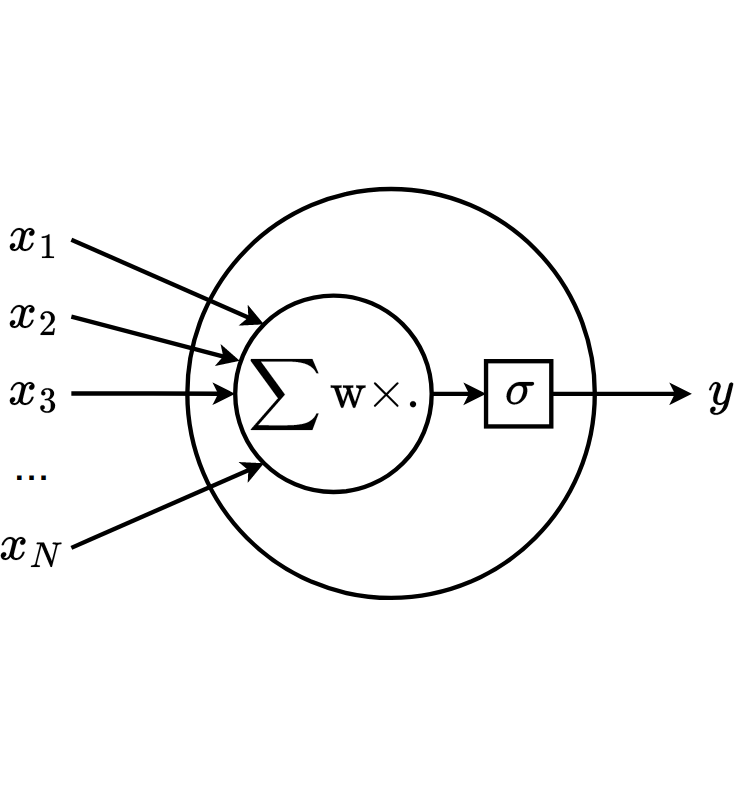
\includegraphics[width=\textwidth]{Figures/RL/perceptron.png}
        \caption{Perceptron}
        \label{fig:perceptron}
    \end{subfigure}
    \hfill
    \begin{subfigure}[b]{0.5\textwidth}
        \centering
        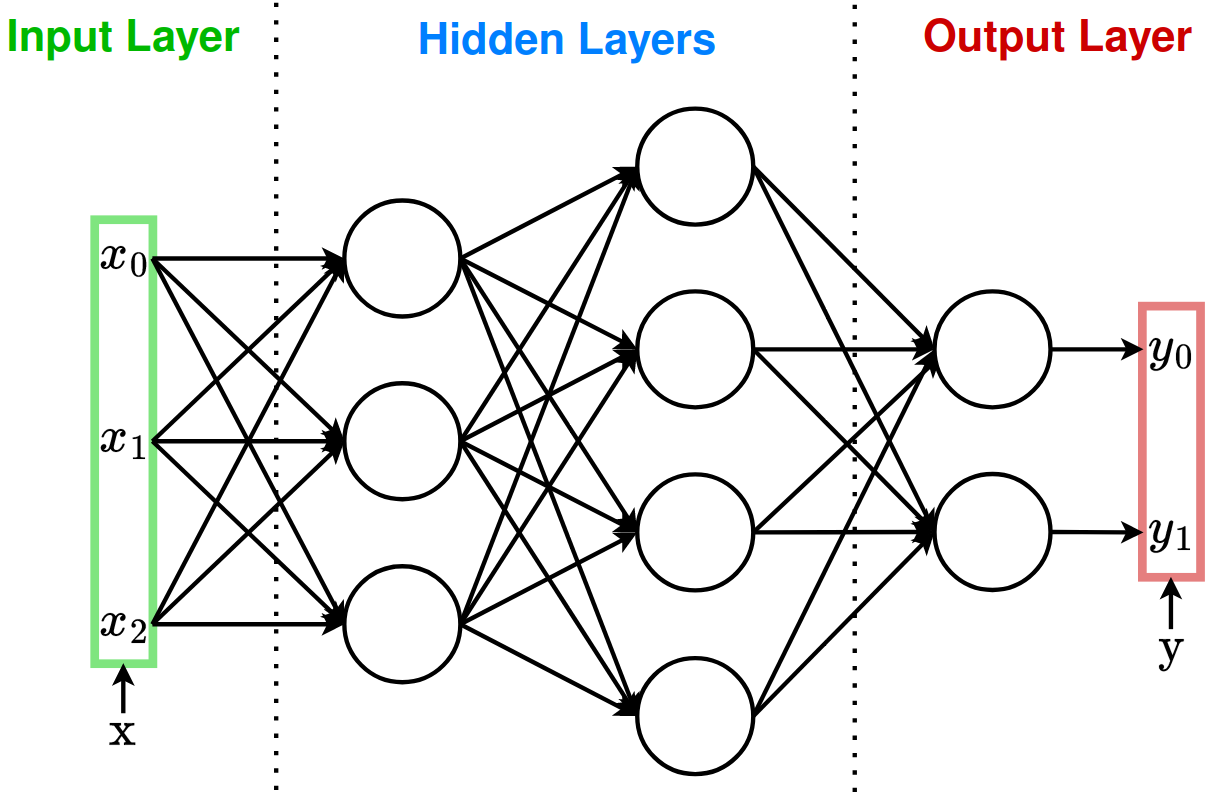
\includegraphics[width=\textwidth]{Figures/RL/mlp.png}
        \caption{Artificial neural network}
        \label{fig:mlp}
    \end{subfigure}
    \hfill
    \caption{Architecture of an artificial neural network (ANN). (a) The perceptron, i.e., the neuron-like element, transforming an input vector into a single output value. It does so with a summed vector multiplication with the neuron's weights $w$ and by using the activation function $\sigma$ that determines the activation of the neuron. (b) Example of ANN, with each circle representing a single perceptron. As there are more than one hidden layer, it is a multi-layer perceptron.}
    \label{fig:ann}
\end{figure}

% ANN
The term \textbf{artificial neural network} (ANN) designates a type of parameterised architecture that can be used to solve machine learning problems. Concretely, an ANN is a mathematical function that transforms the input vector, into an output vector of another form: $f:\mathbb{R}^N\rightarrow\mathbb{R}^M:f(x;\theta)=y$, with $x$ and $y$ respectively the input and output vectors of dimensions $N$ and $M$, and $\theta\in\mathbb{R}^{d^\theta}$ the vector of parameters of the neural network. The name "artificial neural network" comes from the actual form of this function. It can be decomposed into many simpler functions, each one of them acting as a neuron-like activation. The aggregation of multiple of these neurons in a computational graph builds the network architecture of the global function, as illustrated in Figure \ref{fig:mlp}.

% Perceptron
The neuron element of this network, illustrated in Figure \ref{fig:perceptron}, is called a \textbf{perceptron}~\citep{Rosenblatt1958_Perceptron}. It is a simple function that transforms a given input vector $x\in\mathbb{R}^N$ into a single output value $h(x;w)\in\mathbb{R}$ through a weighted sum. In this operation, each element of the input vector is multiplied by a learnable parameter $w_i\in\mathbb{R}$, also called a \textit{weight}, before being all summed together:
\begin{equation}
    h(x;w)=\sum_{i=1}^Nw_ix_i+b,
\end{equation}
with the input vector $x=\{x_i\}_{0<i\leq N}$, the weights $w=\{w_i\}_{0<i\leq N}$, and a bias parameter $b\in\mathbb{R}$. This bias, which is also a learnable parameter, is needed to learn more complex transformations. 

% Activation function
The result of this operation is then passed through an activation function $\sigma$ that determines the final output of the neuron:
\begin{equation}
    y=\sigma\left(h(x;w)\right)=\sigma\left(\sum_{i=1}^Nw_ix_i+b\right).
\end{equation}
This activation function is a non-linear transformation of the input. Without the non-linear activation, an aggregation of perceptrons could be rewritten as a linear transformation of the input. Thus, the purpose of $\sigma$ is to allow the neural network to model non-linear functions. Three examples of frequently used activation functions are the \textit{sigmoid} function, the hyperbolic tangent (\textit{Tanh}), and the Rectified Linear Unit (\textit{ReLU}; \cite{Glorot2011_ReLU}), all shown in Figure~\ref{fig:activ}.

% NN architecture & Parameters
Multiple perceptrons can be used to build a neural network, like in Figure \ref{fig:mlp}. In the classical ANN architecture, the neurons are structured in \textit{layers}. Each layer is composed of a fixed number of neurons, each neuron taking as input all the outputs of the previous layer. For this reason, this kind of layer is often called \textit{fully-connected}. Three distinct parts of the network are often identified: the input layer, the hidden layers, and the output layer. The input layer is made by the input vector. The output layer is the layer of neurons that will generate the output vector. Thus, both the dimensions of the input and output layers are determined by the required dimensions of the input and output vectors. On the other hand, between the input and output layers, the number of hidden layers and neurons in each one of them can be defined arbitrarily. Each neuron has its set of learnable parameters, whose dimension depends on the size of the last layer: one weight for each input, plus the bias. Thus, the parameters of the whole ANN, defined previously as $\theta$, is the set of all parameters (weights and biases) of all neurons in the network. 

% Activation functions
\begin{figure}
    \centering
    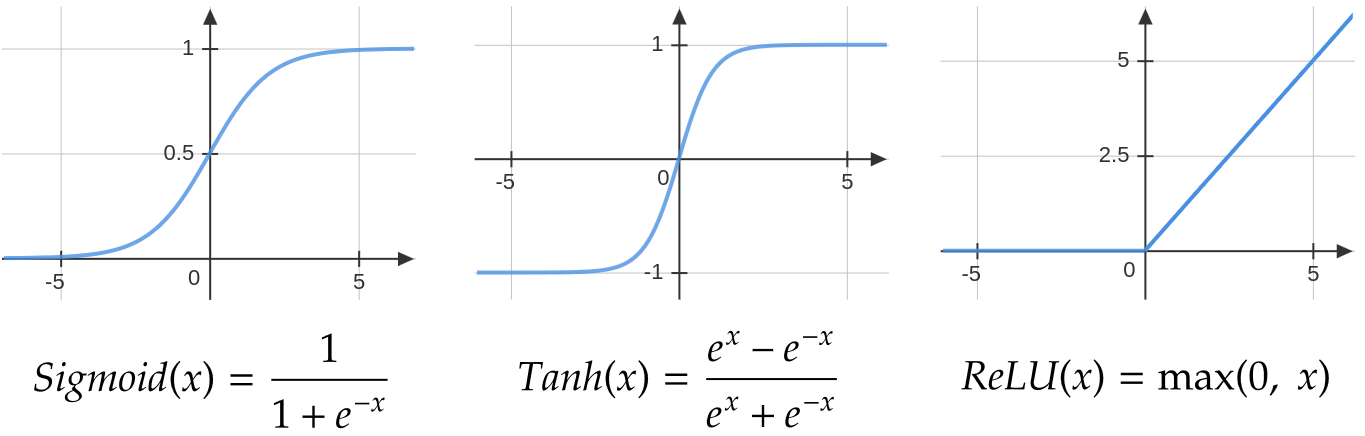
\includegraphics[width=0.9\textwidth]{Figures/RL/activ.png}
    \caption{Mathematical definitions and representations of three activation functions: sigmoid, hyperbolic tangent (Tanh), and rectified linear unit (ReLU).}
    \label{fig:activ}
\end{figure}

% Learning (gradient descent, forward/backward prop)
Learning these parameters can be done with gradient descent. When training the network, training examples $x$ are fed into the network, generating predicted outputs: $\widehat{y}=f(x;\theta)$. This is called the \textit{forward propagation}. The predictions are evaluated by a loss function that measures their quality with regard to the training objective. For example, in a supervised task, the objective of the model is to predict a target value $y$ associated with $x$ in the training data. In this case, the loss function measures the prediction error, which can be defined as the \textit{mean squared error}:
\begin{equation}
    L(\widehat{y};\theta)=\frac{1}{M}\sum_{i=1}^M(y_i-\widehat{y}_i)^2,
\end{equation}
with $M$ the dimension of the output layer. All operations made inside the network (i.e., $f$) are differentiable\footnote{The derivatives of some activation functions may not be defined everywhere (e.g., ReLU in 0), when that is the case, a value is arbitrarily defined for the missing derivatives (e.g., $\text{ReLU}'(0)=0$).}. This allows computing the gradient of the loss $L(\widehat{y};\theta)$ with regard to each parameter in the network, through a series of chain rules. Thus, the parameters can be updated to minimise the loss:
\begin{equation}
    \theta\leftarrow\theta-\alpha\nabla_\theta L(\theta),
\end{equation}
with a learning rate $\alpha\in]0,1]$. Notice the negative sign of the gradient used in gradient descent to minimise the loss, conversely to gradient ascent presented in Section \ref{sec:RL:Policy-based}, which was intended for maximising the RL objective. This process of going back to each parameter in the graph to compute its gradient and update it is often referred to as \textit{backward propagation}, or back-propagation.







\subsection{Recurrent Neural Networks}\label{sec:NN:RNN}

% RNN
The ANN architecture presented previously is one of many other more complex structures that specialise in particular tasks. One limitation of the ANN is that it struggles to handle sequential data, where inputs are arranged in time and can depend on previous inputs. For example, text is a form of sequential data where words and punctuation marks are arranged in a sequence. In this sequence, some words may have a strong correlation with others. In such cases, a neural network would benefit from learning these potential correlations by memorising some information from previous inputs. This is the idea behind \textbf{recurrent neural networks} (RNNs) that propose an architecture for handling sequential data, illustrated in Figure \ref{fig:rnn}. At each time step $t$, the RNN unit takes two inputs: the input data point $x_t\in\mathbb{R}^N$ and the hidden state of the last step $h_{t-1}\in\mathbb{R}^M$. The hidden state is a vector that carries information between each step of the process. At each step, it is updated with:
\begin{equation}
    h_t=\sigma\left(W_xx_t+W_hh_{t-1}+b\right),
\end{equation}
with $W_x\in\mathbb{R}^{N\times M}$ and $W_h\in\mathbb{R}^{M\times M}$ two matrices of learnable parameters, a bias vector $b\in\mathbb{R}^M$, and an activation function $\sigma$, which is often a Tanh in RNNs. The output is then a function of the hidden state: $y_t=g(h_t)$. Here, function $g$ can be a layer of perceptrons to output a vector in the required dimension. The RNN unit serves as a fundamental block that is often used inside a larger architecture. 

Notice that, all the computations made from the beginning of the sequence can be traced back in the final hidden state $h_T$ and written as a function of all inputs of the sequence: $h_T=g(x_T,h_{T-1})=g(x_T,g(x_{T-1},h_{T-2}))$, and so forth. Thus, as for the ANN, we can compute the gradients of a given loss function with regard to each parameter of the RNN unit. The specificity here is that the gradients are "back-propagated through time", as the loss at step $T$ depends on calculations done in all previous steps. This allows the RNN to learn the temporal correlation in the input sequences.

% Figure RNN
\begin{figure}
    \centering
    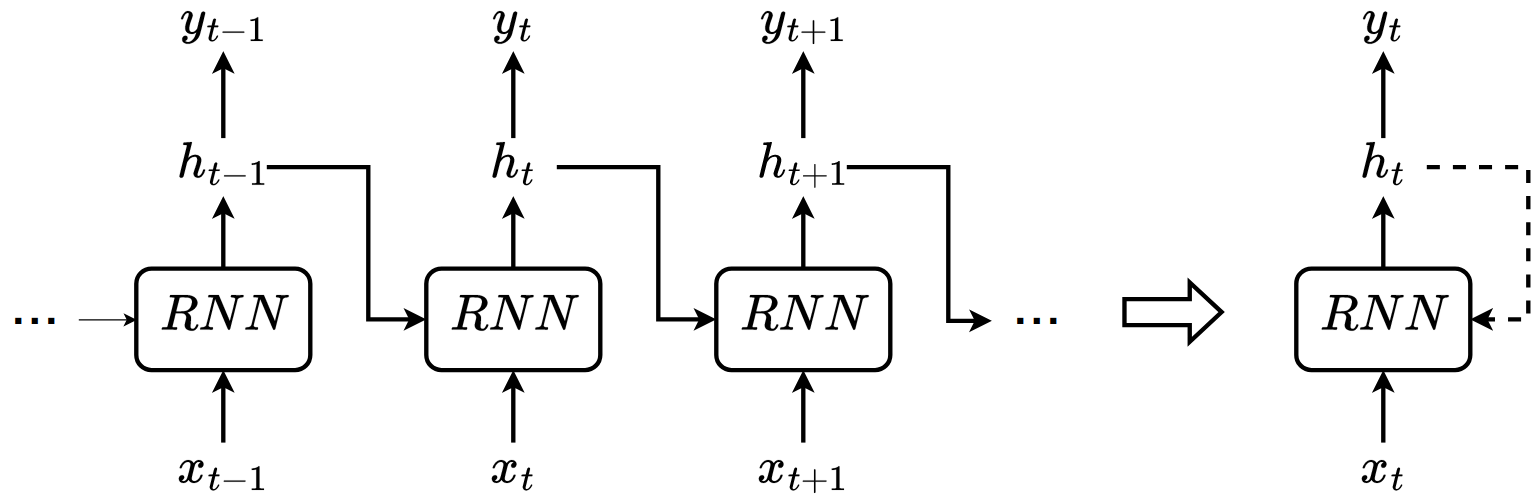
\includegraphics[width=0.8\textwidth]{Figures/RL/rnn.png}
    \caption{Illustration of a recurrent neural network (RNN) unit handling the sequence of inputs $x$. The left version shows the process unfolded in time, with the hidden state of step $t$ passed to the next step $t+1$. On the right is shown a condensed illustration of the RNN, with the dashed arrow indicating that $h_t$ is carried out to the next step.}
    \label{fig:rnn}
\end{figure}

% LSTM - GRU
While the hidden state of the RNN carries some information to the next step, in practice, this simple RNN struggles to memorise long-term information. In addition to that, it suffers from algorithmic flaws that prevent its use in many applications. However, better recurrent architectures have been developed to address these issues. The \textbf{Long Short-Term Memory} (LSTM) architecture~\citep{Hochreiter1997_LSTM} is one example (see Figure \ref{fig:lstm-gru}). Inside the LSTM unit, the information flows into various \textit{gates} that ensure the conservation or forgetting of some parts of the inputs. In addition to the hidden state, a "cell state" is also kept between steps. Intuitively, the cell state should carry more long-term memory than the hidden state. Another similar recurrent architecture is the \textbf{Gated Recurrent Unit} (GRU; \cite{Chung2014_GRU}). The GRU takes inspiration from the LSTM, but simplifies its architecture while keeping similar performance. In practice, both the LSTM and GRU are used in recent works to deal with sequential data. 

% Illustration LSTM et GRU
\begin{figure}
    \centering
    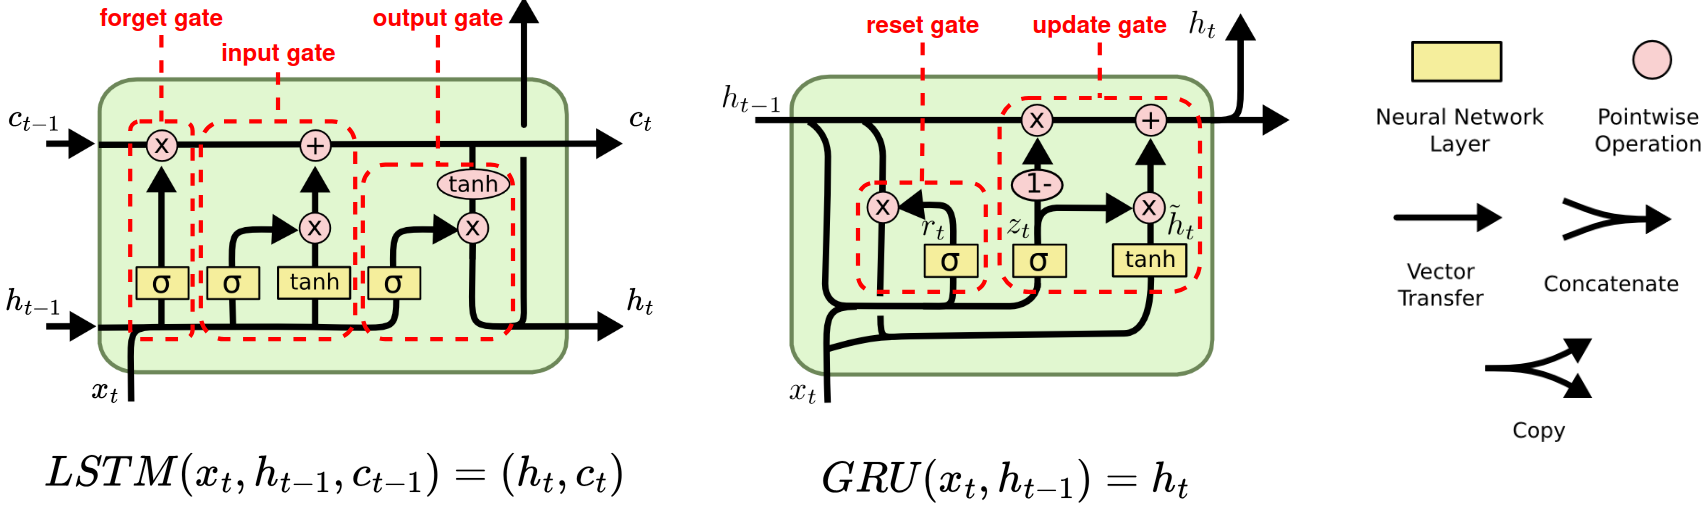
\includegraphics[width=0.9\textwidth]{Figures/RL/lstm-gru.png}
    \caption[LSTM-GRU]{Illustration of the Long Short-Term Memory (LSTM) and Gated Recurrent Unit (GRU) neural network architecture\footnotemark. Input information flows along the black arrows and passes through different "gates". These gates are neural networks that compute the outputs by updating the memory, forgetting some information and adding some new from the input $x_t$. In addition to the hidden state, the LSTM carries the cell state $c$ between each step to extend the memory capacities.}
    % PLACEHOLDER illustration, to do own
    \label{fig:lstm-gru}
\end{figure}

\footnotetext{Illustrations adapted from: \url{http://colah.github.io/posts/2015-08-Understanding-LSTMs/}.}

\subsection{Deep Neural Networks}\label{sec:NN:DeepLearning}

% Learning representations
The great strength of neural networks is their ability to automatically learn hidden relations in the training data. Take for example a computer vision task, where the objective is to determine the presence of a car in images. Classical machine learning algorithms usually require high-level features to solve such tasks: the presence of wheels in the picture, the number of such wheels, the presence of reflective material, and other common attributes of cars. With neural networks, such high-level features can be extracted automatically by looking at the training data. This is called \textit{representation learning}, where the neural network learns a set of weights (as described in Section \ref{sec:NN:ANN}) that produces accurate internal representations of the input data. Through careful training, the network learns how to understand the information given in the picture, to give an accurate prediction of the presence of a car. Because this is done automatically, this relieves the otherwise painful work of manually extracting and annotating important features in all training samples. This also allows the neural network to discover hidden features that could have been omitted in human-generated data (e.g., the fact that cars are often pictured on a road, so the presence of road signs might increase the probability of having a car in the image). However, there are also downsides to this. First, this automatic process of learning representations is done in a black box that is out of the control of human observers. The representation capacities of the neural network are embedded in the weights of the networks and are hard to understand and interpret. Second, these representation capacities still have a cost, now measured in the amount of training data at our disposal. To learn the complex relations in a very large space of input values and obtain good performance, neural networks usually require very large datasets of standardised data. Still, obtaining these datasets is often less difficult than manually extracting valuable features by hand. 

% MLP
It has been widely recognised that the number of layers in a neural network can greatly influence its performance in solving the task. In many cases, adding hidden layers can improve the representations learnt by the network. This can be understood intuitively by looking at each layer as a representation unit, where the first layer extracts low-level information, and subsequent layers each use the representation given by the last layer to extract more high-level features. This has led to the use of \textit{deep neural networks} that have more than one hidden layer, as in Figure \ref{fig:mlp}. These networks, often called \textbf{Multi-Layer Perceptrons} (MLPs), are the fundamental block of what is now called \textit{deep learning}, corresponding to any machine learning architecture that features deep neural networks.  

% Various Techniques and architectures (CNN, Attention, Transformers,...)
The MLP is the most basic form of deep neural architecture. It is often used to handle any input that can be represented as a vector. But, other architectures have been developed for specific types of inputs. For sequential data, the RNNs can be extended to have a deep architecture, with many recurrent units stacked on top of each other, as in Figure \ref{fig:deep-rnn}. For images, the \textbf{Convolutional Neural Networks} (CNNs; \cite{LeCun1989_CNN, Krizhevsky2012_AlexNet, Simonyan2015_VGG}) learn to detect complex patterns of pixel values that can then be used to recognise objects in images (see Figure \ref{fig:cnn}). Recently, the Transformer architecture~\citep{Vaswani2017_Transformer} have been introduced to handle sequential data, with better long-term memory than recurrent architectures. Transformers have been widely adopted in the machine learning community as a foundation for building better models. Extremely large Transformers with billions of learnable parameters have demonstrated superior performance in text generation~\citep{Ouyang2022_InstructGPT} and computer vision~\citep{Dosovitskiy2021_VisionTransformer}.

\begin{figure}
    \centering
    \hfill
    \begin{subfigure}[b]{0.3\textwidth}
        \centering
        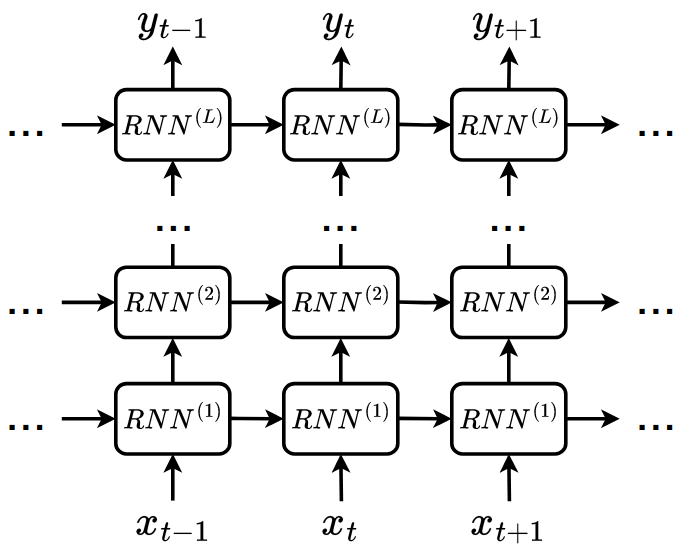
\includegraphics[width=\textwidth]{Figures/RL/deep-rnn.png}
        \caption{Deep RNN}
        \label{fig:deep-rnn}
    \end{subfigure}
    \hfill
    \begin{subfigure}[b]{0.6\textwidth}
        \centering
        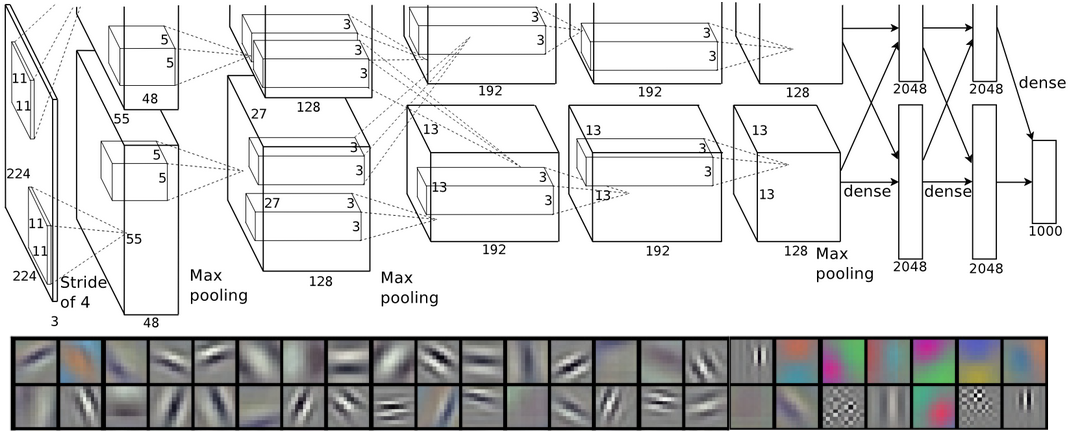
\includegraphics[width=\textwidth]{Figures/RL/vgg.png}
        \caption{Deep CNN}
        \label{fig:cnn}
    \end{subfigure}
    \hfill
    \caption{Two examples of deep neural network architectures. (a) A deep RNN, where the input $x_t$ passes through $L$ RNN units to compute the output $y_t$, with each unit passing its hidden state $h^{(i)}_t$ to the next layer $i+1$ and to the next step $t+1$. (b) Architecture of a deep convolutional network on top, and the bottom shows the learnt filters of the first convolutional layer that detect basic shapes in the images~\citep{Simonyan2015_VGG}.}
    \label{fig:ann}
\end{figure}

% Issues and hyperparameters
Overall, the impact of deep neural networks on machine learning has been tremendous. In the next section, we will see that deep learning is now a common technique in reinforcement learning research. But it also comes with its share of complications. First, training deep neural networks requires large amounts of data to train on. A larger neural network usually needs more data to train efficiently~\citep{Kaplan2020_ScalingLaws} and a common trend of greatly increasing model sizes to improve performance has been observed~\citep{Villalobos2022_ModelSizes}. Training larger models requires considerable computational power and access to computers equipped with Graphics Processing Units (GPUs) that can efficiently compute large matrix operations. This makes deep learning expensive and not accessible to anyone with a restricted budget. Even executing a trained model requires some computational capacities, which makes deployment on small platforms (e.g., robots) complicated. Lastly, deep neural networks are often complex and depend on many design choices to function well. They usually come with a long list of parameters, often called \textit{hyperparameters} to distinguish them from learnable parameters, that define their architecture and training setting: the number of layers, the dimension of the hidden layers, the learning rate, etc. Each one of these hyperparameters is a value that can impact the performance of the model and that needs to be tuned. But, despite these obstacles, deep learning is now widely used in artificial intelligence research and its applications, and is now a common building block of all state-of-the-art approaches in domains like computer vision and natural language processing.





% -------------------------------------------------------------------------




\section{Model-Free Deep Reinforcement Learning}\label{sec:DRL}

As in other branches of machine learning, deep learning has been a revolutionary technique for RL. It has enabled extending existing RL algorithms to operate in much more complex settings and has facilitated the development of new approaches for learning models, policies, and value functions. In this section, we will present the foundational works in model-free deep RL published in the last decade. These works form the basis for the majority of studies in both single-agent and multi-agent RL. While there is also significant research on model-based deep RL methods~\citep{Moerland2023_ModelRL}, we will not cover them here as they are not typically used in multi-agent settings and are thus outside the scope of this thesis. 


\subsection{Value-Based Methods}

\subsubsection{Deep Q-Learning}\label{sec:DRL:DQN}

% Motivations
In Section \ref{sec:RL:Qlearning}, we presented the Q-learning algorithm for learning a control policy using only an action-value function. We introduced the main limitations of this algorithm: scalability and generalisation. First, tabular Q-learning scales poorly to environments with large state-action spaces, as it needs to keep track of the learnt values of all state-action pairs. Second, Q-learning struggles to generalise its training knowledge to make good predictions in situations it has never experienced. It needs a thorough exploration of the environment to ensure that its predicted values are relevant. For these reasons, Q-learning is difficult to use in realistic settings where the number of possible states is large or infinite. 

These issues can be alleviated using a deep neural network in place of the value table. The \textbf{Deep Q-Network} (DQN), proposed by \cite{Mnih2013_DQN}, successfully adapts Q-learning to learn from visual data. To do so, it models the action-value as a CNN (see Section \ref{sec:NN:DeepLearning}) that takes as input frames from a video game and outputs the values of possible actions, as illustrated in Figure~\ref{fig:dqn}. Note that, while this first iteration of the DQN architecture uses a CNN, the term DQN is now used to describe any deep neural network architecture that computes action-values. 

The DQN is learnt completely end-to-end from the Q-learning objective. Concretely, the parameters of the network $\theta$ are optimised to minimise the following squared Bellman error:
\begin{equation}
    L(\theta)=\left(r_{t+1}+\gamma\max_{a}Q_{{\theta^-}}(s_{t+1},a)-Q_\theta(s_t,a_t)\right)^2,
\end{equation}
for any transition $\langle s_t,a_t,r_{t+1},s_{t+1}\rangle$ and with the discount factor $\gamma$. Notice the TD-target is computed using another network $Q_{\theta^-}$, named the \textit{target network}. The parameters $\theta^-$ are initialised as a copy of the main parameters $\theta$. Then, the target is fixed for a pre-defined number of training iterations, after which it is copied from the main network again, and so on. Using a slightly older, fixed version of $Q_\theta$ helps to stabilise training by giving a fixed target to aim for when minimising the Bellman error, instead of having it modified after each training iteration~\citep{Mnih2015_DQN}. 

% Experience replay
Another important feature of the DQN is its use of experience replay~\citep{Lin1992_ExperienceReplay}. Because deep Q-learning is off-policy, it can capitalise on all previously acquired experiences to train its deep neural network. The deep Q-learning algorithm thus alternates between acquiring experiences by interacting with the environment (typically executing the $\epsilon$-greedy policy), storing each experience in the replay buffer $\mathcal{B}$, and later training the DQN on a batch of samples randomly drawn from $\mathcal{B}$. Therefore, the DQN is trained to minimise the Mean Squared Bellman Error (MSBE) on the full batch:
\begin{equation}
    L(\theta)=\mathbb{E}_{\langle s,a,r,s'\rangle\sim\mathcal{B}}\left[\left(r+\gamma\max_{a'}Q_{{\theta^-}}(s',a')-Q_\theta(s,a)\right)^2\right].
    \label{eq:DQN}
\end{equation}
This batched loss is crucial for ensuring efficient training of a deep neural network. Plus, experience replay allows reusing each gathered experience multiple times and having more diverse batches, thus improving sample efficiency and avoiding overfitting the current policy.

DQN was the first successful instance of coupling RL with deep learning. It showed that deep RL was able to surpass human performance in video games, by learning only from visual data~\citep{Mnih2013_DQN}. It sparked a wave of research focused on using deep learning in existing RL algorithms and developing new learning methods specific to deep RL. 

\begin{figure}
    \centering
    \hfill
    \begin{subfigure}[b]{0.64\textwidth}
        \centering
        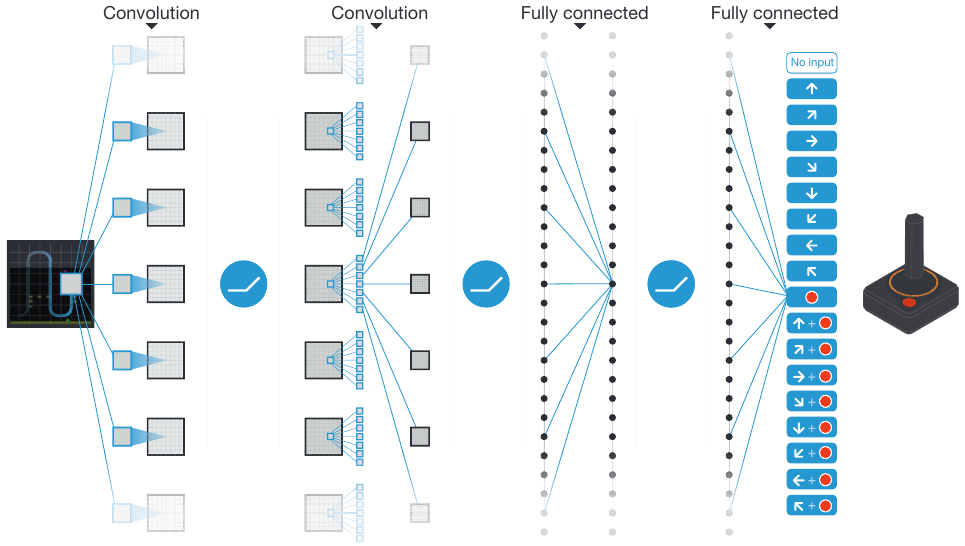
\includegraphics[width=\textwidth]{Figures/RL/dqn.png}
        \caption{Deep Q-Network}
        \label{fig:dqn}
    \end{subfigure}
    \hfill
    \begin{subfigure}[b]{0.35\textwidth}
        \centering
        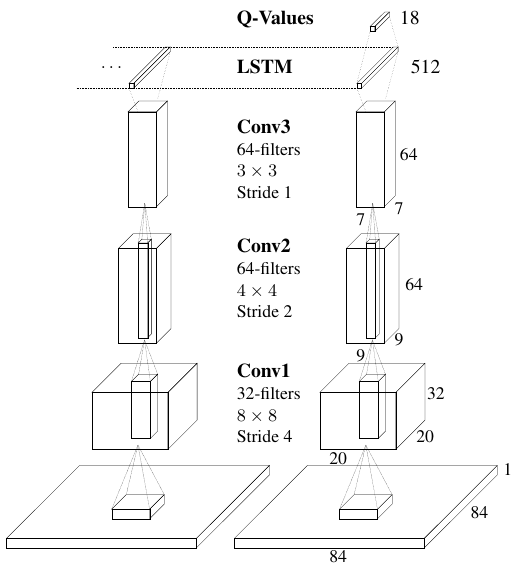
\includegraphics[width=\textwidth]{Figures/RL/drqn.png}
        \caption{Deep Recurrent Q-Network}
        \label{fig:drqn}
    \end{subfigure}
    \caption{DQN architectures. (a) The original DQN~\citep{Mnih2015_DQN}, with a series of convolution layers that analyse the input frame, followed by fully connected layers that output the value of each action. (b) Recurrent version of a DQN~\citep{Hausknecht2015_DRQN}, that adds an LSTM unit after the convolutions to allow some information to carry to future steps.}
    \label{fig:dqns}
\end{figure}



\subsubsection{DQN Extensions}\label{sec:DRL:Rainbow}

Following the introduction of the DQN, many works focused on improving this architecture using both old and new techniques. In their paper, \citet{Hessel2018_Rainbow} summarise the most important extensions and combine them into their method called \textit{Rainbow}. Some of these improvements concern the core functioning of the Q-learning algorithm:
\begin{itemize}
    \item \textit{Double Q-learning}~\citep{Hasselt2010_DoubleQlearning} modifies Equation~\ref{eq:DQN} to decouple the selection of the action to its evaluation when computing the Bellman error:
    \begin{equation}
        L(\theta)=\Bigl(r_{t+1}+\gamma Q_{{\theta^-}}(s_{t+1},\argmax_{a'}Q_\theta(s_{t+1},a'))-Q_\theta(s_t,a_t)\Bigl)^2.
        \label{eq:DDQN}
    \end{equation}
    In the TD-target, the action is selected by the main network $Q_\theta$ and evaluated by the target network $Q_{\theta^-}$. \citet{Hasselt2016_DoubleDQN} apply this idea to the DQN to improve its performance.

    \item The \textit{Dueling DQN}~\citep{Wang2016_DuelingDQN} proposes to decompose the action-value of an action $Q_(s,a)$ into two separate predictions: the value of the current state $V(s)$ and the \textit{advantage} of the action defined as $A(s,a)=Q(s,a)-V(s)$. They use a neural network architecture with two outputs, the state-value and advantage, which are then combined into the action-value. This allows them to learn a state-value and an action-value function in a single learning process with a deep Q-learning algorithm. 

    \item \textit{Distributional value learning}~\citep{Bellemare2017_DistributionalRL} proposes to learn a probability distribution over possible future returns, instead of learning to estimate the expected return of an action. Doing this allows to better account for multimodality in value distributions and generally improves learning stability. 
\end{itemize}
Other techniques focus on algorithmic and architectural improvements to DQN:
\begin{itemize}
    \item \textit{Prioritised experience replay}, proposed by \citet{Schaul2016_PER}, improves on experience replay by sampling experiences more often if they lead to bad value predictions (i.e., high Bellman errors) during training. This allows prioritising samples that the network fails to evaluate well, thus greatly improving sample efficiency. 

    \item \textit{Noisy DQN}~\citep{Fortunato2018_NoisyDQN} tackles the problem of exploration by adding noise to the parameters of the DQN. Note that \citet{Plappert2018_Noise} concurrently proposed a similar approach working with other deep RL algorithms. 
\end{itemize}
Rainbow shows that combining all these extensions greatly improves the performance and sample efficiency of DQN in a large variety of video games~\citep{Hessel2018_Rainbow}. 

\subsubsection{Deep Recurrent Q-Network}\label{sec:DRL:DRQN}

A remaining limitation of DQN is its lack of memory of previous events. This becomes a problem in partially observable environments where the agent does not get the full state of the environment, but rather a local observation describing its surroundings. In such settings, a memory-equipped agent could explore its surroundings to build a better understanding of the current state of the environment. To achieve this, \citet{Hausknecht2015_DRQN} augment the DQN architecture with an LSTM unit (see Section \ref{sec:NN:RNN}) to learn to memorise important information for future steps (see Figure~\ref{fig:drqn}). They show that this makes agents more robust to losses in their observations. This approach has been combined with distributed training by \citet{Kapturowski2018_R2D2}, largely surpassing previous works on some Atari games. As we will see in Chapter \ref{ChapterMADRL}, using recurrent units has been widely adopted in multi-agent deep RL to deal with partial information given to each agent. 





\subsection{Policy-Based Methods}\label{sec:DRL:Policy}

\subsubsection{Deep Deterministic Policy Gradient}\label{sec:DRL:DDPG}

% DDPG
In Section \ref{sec:Policy:Actor-Critic}, we introduced the actor-critic architecture that combines a policy (i.e., actor) and a value (i.e., critic) to open up the possibilities of RL training. Following the introduction of the DQN, similar ideas were implemented to extend actor-critics with deep learning. The \textbf{Deep Deterministic Policy Gradient} (DDPG; \cite{Lillicrap2015_DDPG}) was proposed to extend the DQN to work with continuous actions. Like in the original DPG (see Section \ref{sec:Policy:Actor-Critic}), a deterministic policy function $\pi_\theta$ is learnt to select actions in a continuous space and an action-value function $Q_\phi$ is used to predict the quality of the selected actions. Here, both of these are modelled using deep neural networks. As in Double Q-learning (see Section \ref{sec:DRL:Rainbow}), both the policy and value functions are doubled with target functions $\pi_{\theta^-}$ and $Q_{\phi^-}$, respectively. The targets are used to compute the TD-target for computing the MSBE loss:
\begin{equation}
    L(\Theta)=\mathbb{E}_{\langle s,a,r,s'\rangle\sim\mathcal{B}}\left[\left(r+\gamma Q_{\phi^-}(s',\pi_{\theta^-}(s'))-Q_\phi(s,a)\right)^2\right].
    \label{eq:DDPG}
\end{equation}
The target parameters $\Theta^-=\{\theta^-,\phi^-\}$ are initialised as copies of the main parameters $\Theta$ and later slowly moved towards the main networks with a "soft" update: $\Theta^-\leftarrow\tau\Theta^-+(1-\tau)\Theta$, with $0<\tau\ll1$. Using this approach, combined with experience replay and other small tricks, DDPG managed to greatly improve on the non-deep DPG. 

% TD3
\citet{Fujimoto2018_TD3} pointed out that DDPG, as all Q-learning methods, suffers from an overestimation of action-values induced by using a bad value estimate for computing the optimisation objective. While Double Q-learning helps address this issue, it does not completely solve it. They propose an extension of DDPG, named \textit{Twin Delayed DDPG} (TD3), that better mitigates the overestimation problem with three tricks:
\begin{itemize}
    \item First (\textit{Twin}), TD3 learns two action-value functions instead of one and uses the smaller values of the two when computing the TD-target. 
    \item Second (\textit{Delayed}), the policy function is trained less often than the action-value functions (one policy update for every two value updates) to make the policy less prone to value errors. 
    \item Third, the value estimates are smoothed by adding a small clipped noise on the target policy actions when computing the TD-target. This prevents having high spikes of value on some particular actions that the deterministic policy would then overfit to.
\end{itemize}
Therefore, TD3 computes the TD-target by taking the minimum value given by the twin DQNs and adding the clipped noise to the policy's action:
\begin{gather}
    y(r,s')=r+\gamma\min_{i=1,2}Q_{\phi_i^-}(s',\pi_{\theta^-}(s')+\epsilon), \\
    \epsilon\sim\text{clip}(\mathcal{N}(0,\sigma),-c,c),
\end{gather}
for some transition $\langle s,a,r,s'\rangle$, with hyperparameters $\sigma$ and $c$ controlling the width of the smoothing noise. The twin DQNs are both trained to minimise their MSBE:
\begin{equation}
    L(\phi_i)=\mathbb{E}_{\langle s,a,r,s'\rangle\sim\mathcal{B}}\left[\left(y(r,s')-Q_{\phi_i}(s,a)\right)^2\right], \text{ with } i\in\{1,2\}.
\end{equation}
These modifications are shown to improve the stability and performance of DDPG.


% \subsubsection{Asynchronous Advantage Actor Critics}

\subsubsection{Trust Region Policy Updates}\label{sec:DRL:PPO}

% Policy gradient limitations
In Section~\ref{sec:Policy:PolicyGradientTheorem}, we presented the policy gradient method used in most policy-based algorithms, which aims at maximising the following objective for learning a stochastic policy:
\begin{equation}
    L^{PG}(\theta)=\mathbb{E}_\pi\left[\log\pi_\theta(a|s)Q_{\pi_\theta}(s,a)\right].\footnote{If we compute the gradient of this objective, we find the formulation of Equation~\ref{eq:PolicyGradient:sampleA} as, by chain rule, $\nabla_x\log f(x)=\frac{\nabla_xf(x)}{f(x)}$.}
\end{equation}
This objective has two important limitations. First, the size of the learning step is difficult to define. In the context of learning a policy that generates the data it is trained on, a too big learning step could be catastrophic if it engenders a bad policy. In supervised learning, a bad learning step can be recovered later because the training data is still good. Here, a bad policy would change the distribution of samples and could then be very hard to recover from. Second, this objective theoretically limits the algorithm to use each gathered experience only one time (\cite{Schulman2017_PPO} shows doing multiple updates damages performance), which makes policy gradient algorithms less sample efficient. 

% TRPO
% propose new objective with pi_old, good estimate of PG if pi_old is close to pi
% constraint on KLdiv to ensure that pi doesn't go too far from pi_old
% minimax objective
\citet{Schulman2015_TRPO} propose to modify the policy gradient objective to tackle these issues. The objective is replaced by the following surrogate objective:
\begin{equation}
    L^{surr}(\theta)=\mathbb{E}_{\pi_\theta}\left[\frac{\pi_\theta(a|s)}{\pi_{\theta_{old}}(a|s)}A_{\pi_\theta}(s,a)\right],
    \label{eq:DRL:TRPO-surr}
\end{equation}
where $\pi_{\theta_{old}}$ is another policy and $A_{\pi_\theta}$ is the advantage function defined as $A_\pi(s,a)=Q_\pi(s,a)-V_\pi(s)$~\citep{Baird1995_ResidAlgs}. Using the advantage is equivalent to the action-value but reduces the variance of the value estimate. This objective is shown to be a good approximation of the policy gradient one, only if $\pi_{\theta_{old}}$ is close to $\pi_\theta$. Thus, for this to work, a constraint must be added to ensure that $\pi_\theta$ does not diverge too much from the old version:
\begin{equation}
    \mathbb{E}_{\pi_\theta}\left[KL(\pi_{\theta_{old}}(\cdot|s),\pi_\theta(\cdot|s))\right]\leq\delta,
    \label{eq:DRL:TRPO-constraint}
\end{equation}
with $KL$ measuring the Kullback-Leibler divergence between the two distributions and $\delta$ a hyperparameter for controlling the amount of allowed divergence. Maximising $L^{surr}$ while respecting the constraint of (\ref{eq:DRL:TRPO-constraint}) ensures that the update stays in a "trust region". The resulting \textbf{Trust Region Policy Optimisation} (TRPO) algorithm can do multiple updates on one sampled experience, with $\pi_{\theta_{old}}$ being the policy used when gathering the experience, to improve $\pi_\theta$ as much as possible for each interaction with the environment.

% PPO (... many update per sample), 
% ?Intuitive idea of ppo (going in the direction of good updates)
% improvements on PPO and implementations tricks
While the approach TRPO has great advantages, its implementation is difficult, mainly because of the constraint on KL divergence second-order optimisation. To simplify this, \textbf{Proximal Policy Optimisation} (PPO; \cite{Schulman2017_PPO}) removes the constraint and instead clips the objective to limit the magnitude of the updates. The new, clipped objective is defined as follows:
\begin{equation}
    L^{clip}(\theta)=\mathbb{E}_{\pi_\theta}\left[\min(r(\theta)A_{\pi_\theta}(s,a),\text{clip}(r(\theta),1-\epsilon,1+\epsilon)A_{\pi_\theta}(s,a)\right],
    \label{eq:PPO-objective}
\end{equation}
with $r(\theta)$ the probability ratio from TRPO, $r(\theta)=\frac{\pi_\theta(a|s)}{\pi_{\theta_{old}}(a|s)}$, and $\epsilon$ a hyperparameter typically close to 0. This objective first clips the ratio to be close to 1 to ensure that the new policy does not diverge too much from the old one. Then, they take the minimum of the clipped and unclipped objectives to make a lower bound of the unclipped objective. This objective is simpler to compute and optimise, making PPO simpler to implement. The full objective maximised by PPO is the following:
\begin{equation}
    L^{PPO}(\theta,\phi)=\mathbb{E}_{\pi_\theta}\left[L^{clip}(\theta)-c_1L^{VF}(\phi)+c_2H(\pi_\theta)\right]
    \label{eq:PPOloss}
\end{equation}
where $c_1$ and $c_2$ are coefficients for the two secondary losses. $L^{VF}$ is the MSBE loss for learning the value function used to compute the advantage in (\ref{eq:PPO-objective}), using a technique called Generalised Advantage Estimation~\citep{Schulman2016_GAE}. The third term uses the entropy of the policy, defined as $H(\pi)=\mathbb{E}_\pi[-\log\pi(a|s)]$, to induce exploration. Maximising entropy means increasing the randomness of the policy. This bonus ensures random exploration of new policies. The main objective $L^{clip}$ evaluates each modification with regard to expected future returns. 

PPO is considered one of, if not the best existing deep RL algorithm. It has been deeply studied and improved in various ways since its first release. Many implementation tricks have been identified to be crucial to the performance of the algorithm~\citep{Hendersion2018_Matters, Engstrom2020_PPOImplement}. 



\subsubsection{Soft Actor-Critic}\label{sec:DRL:SAC}

% combine maximum entropy & soft q learning
Finally, we present the Soft Actor-Critic (SAC) algorithm~\citep{Haarnoja2018_SAC} that tackles the poor sample efficiency of on-policy algorithms and the brittleness of off-policy algorithms with regard to their hyperparameters. To do so, it builds an off-policy actor-critic algorithm with a stochastic policy and a "soft" action-value function. The policy is trained on samples drawn from the replay memory $\mathcal{B}$ to maximise the expected future rewards and an entropy bonus for exploration, as in PPO:
\begin{equation}
    L^\pi(\theta)=\mathbb{E}_{s\sim\mathcal{B},a\sim\pi_\theta}\left[Q_\phi(s,a)+\alpha H(\pi_\theta)\right],
\end{equation}
with $alpha$ controlling the importance of the entropy bonus. As in DDPG, the action is sampled from the policy and evaluated by the value function. Maximising this objective operates a trade-off between generating actions with high action-values and inducing diverse behaviours. 

To learn the action-value function, the authors take inspiration from soft Q-learning~\citep{Haarnoja2017_SoftQLearning}, where entropy maximisation is included in the value learning algorithm. The soft action-value is trained to minimise the soft MSBE for any transition drawn from the buffer:
\begin{equation}
    L^Q(\phi)=\mathbb{E}_{\langle s,a,r,s'\rangle\sim\mathcal{B}}\left[\frac{1}{2}\big(Q_\phi(s_t,a_t)-y^{soft}(r,s')\big)^2\right],
\end{equation}
where
\begin{equation}
    y^{soft}(r,s')=r+\gamma\mathbb{E}_{a'\sim\pi_\theta}[Q_\phi(s',a')-\alpha\log\pi_\theta(a'|s')].
\end{equation}
The target in this objective also has a bonus on the entropy of the policy, which makes the action-value function favour actions where the policy is uncertain. They show that this use of entropy maximisation with a stochastic policy greatly improves the stability and robustness of their algorithm. 



% \subsection{Model-based methods}\label{sec:DRL:Model}

% \subsubsection{Planning with Deep RL}\label{sec:DRL:Planning}

% \subsubsection{World models}\label{sec:DRL:WorldModels}





% -------------------------------------------------------------------------

% Conclusion du chapitre (?)
% "on a pas parlé de tout mais présenté les tehcniques qu'on utilise et le domaine du RL dans lequel on se situe"

\section{Conclusion}

In this chapter, we have presented the field of reinforcement learning for training a single agent to solve tasks from its own experience. Understanding the different techniques behind reinforcement learning algorithms is important to understand the challenges we will face later: \textit{how having multiple agents will impact learning} and \textit{how we can use and shape these learning algorithms to fit the requirements of robotic settings}. In the next chapters, we will investigate these issues and propose new approaches for tackling them. 
\Chapter{Multi-Agent Deep Reinforcement Learning in the context of Robotics}{Bridging the gap between MADRL research and robotics}
\label{ChapterMADRL} 




% Figure multi-agent environments (prisonner's dilemma -> pred-prey/foraging -> Hanabi -> SMAC/Dota -> Multi-robot warehouse -> HRI)
\begin{figure}[h]
    \centering
    \begin{subfigure}[c]{0.24\textwidth}
        \centering
        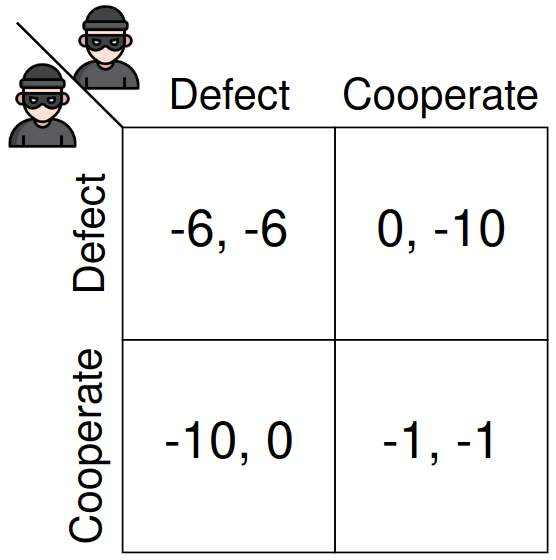
\includegraphics[width=\textwidth]{Figures/MADRL/prisonersdilema.png}
        \caption{Social dilemma}
        \label{fig:prisoners}
    \end{subfigure}
    \hfill
    \begin{subfigure}[c]{0.23\textwidth}
        \centering
        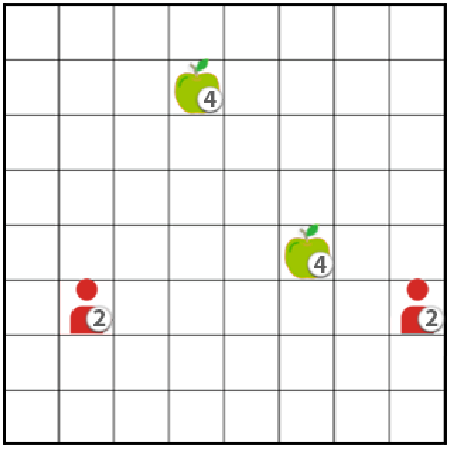
\includegraphics[width=\textwidth]{Figures/MADRL/lbf.png}
        \caption{Two-dimensional grid world}
        \label{fig:lbf1}
    \end{subfigure}
    \hfill
    \begin{subfigure}[c]{0.4\textwidth}
        \centering
        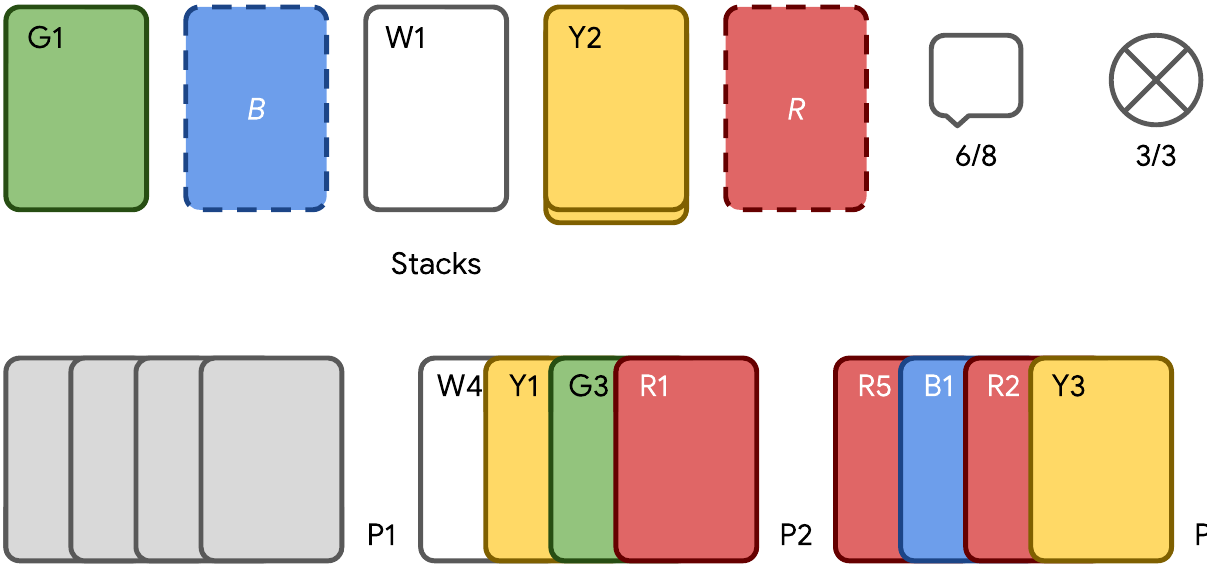
\includegraphics[width=\textwidth]{Figures/MADRL/hanabi.png}
        \caption{Card game}
    \end{subfigure}
    
    \begin{subfigure}[c]{0.32\textwidth}
        \centering
        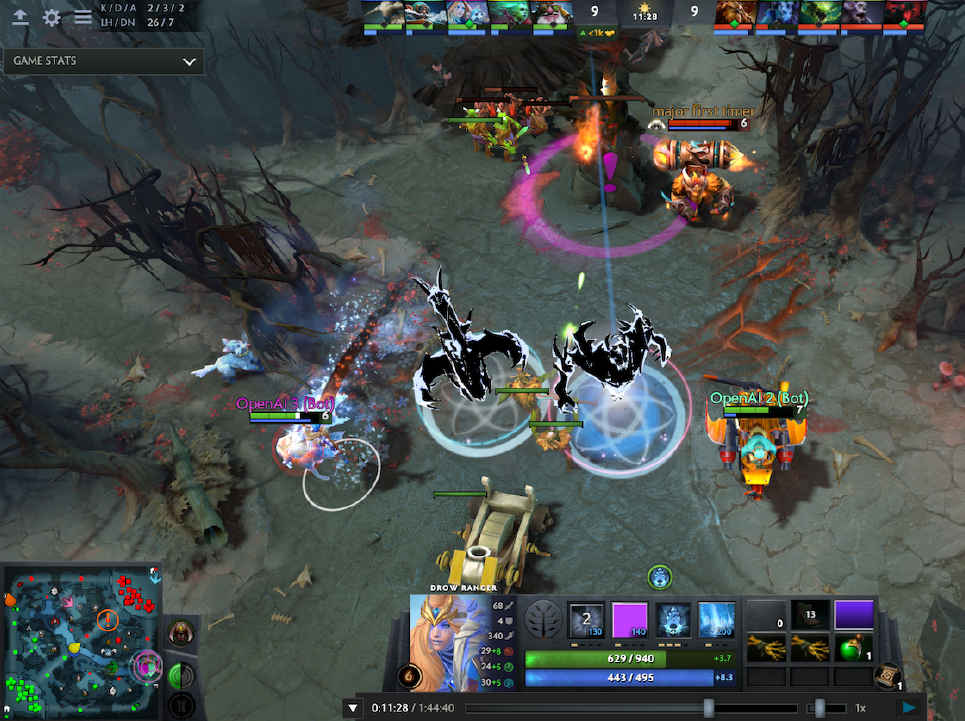
\includegraphics[width=\textwidth]{Figures/MADRL/openaifive.png}
        \caption{Multi-player video game}
        \label{fig:Dota2}
    \end{subfigure}
    \hfill
    \begin{subfigure}[c]{0.35\textwidth}
        \centering
        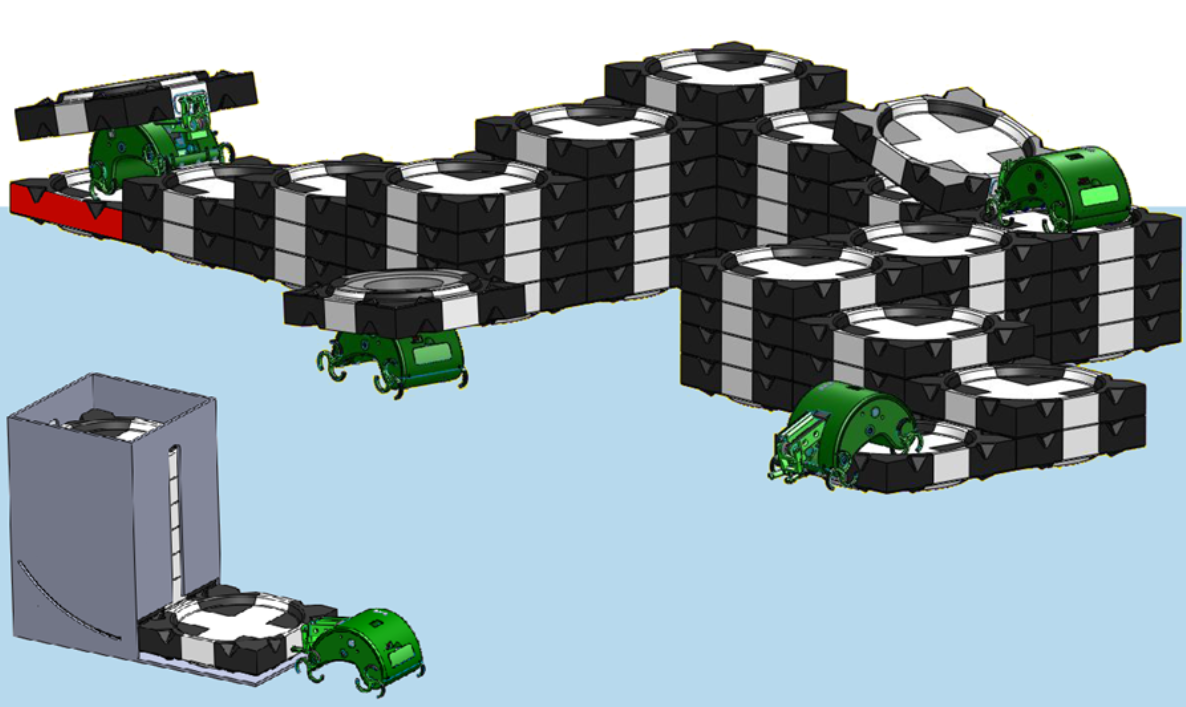
\includegraphics[width=\textwidth]{Figures/MADRL/termes.png}
        \caption{Multi-robot system}
        \label{fig:termes}
    \end{subfigure}
    \hfill
    \begin{subfigure}[c]{0.27\textwidth}
        \centering
        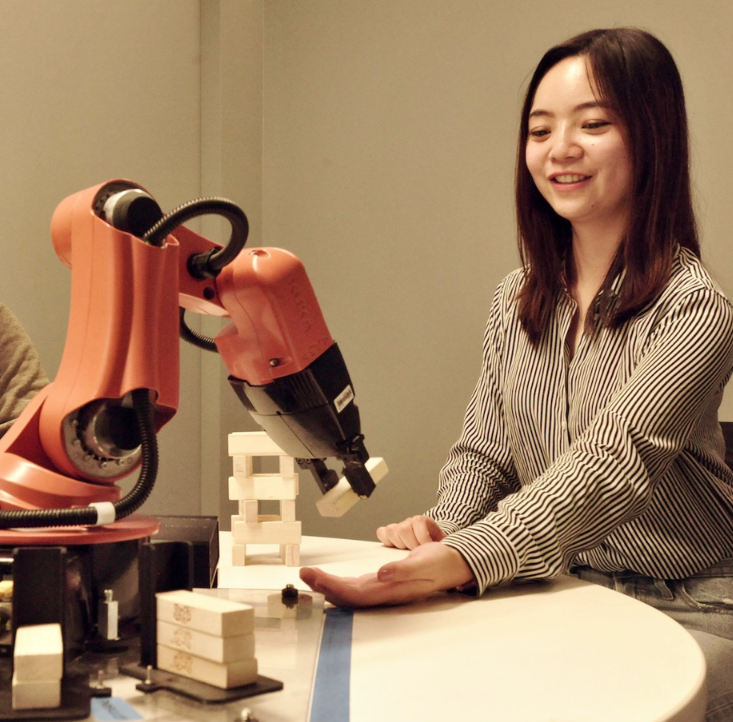
\includegraphics[width=\textwidth]{Figures/MADRL/hri.png}
        \caption{Human-robot interaction}
        \label{fig:hri}
    \end{subfigure}
    \caption{Types of multi-agent environments. (a) Social dilemmas, here the famous \textit{prisoners' dilemma}, extensively used in the game theory literature to devise multi-agent learning concepts and exact solutions. (b) Two-dimensional grid environments (here, level-based foraging;~\cite{Albrecht2013_Foraging}) that allow studying various multi-agent tasks in simplified settings. (c) Card and tabletop games (here, Hanabi;~\cite{Bard2020_Hanabi}) that often require learning complex strategies. (d) Multi-player video games (here, Dota 2, tackled by~\cite{OpenAI2019_DOTA2}) that offer rich environments demanding complex team-play. (e) Multi-robot systems (here, the TERMES construction robots;~\cite{Petersen2012_TERMES}), having to deal with high-dimensional robotic settings. (f) Human-robot interaction, with the need to build interfaces and adapt to human partners~\citep{Jung2020_TowerConstruct}.} 
    \label{fig:MAenvs}
\end{figure}


\section{Introduction}

% Why MAS and MAL
In most realistic environments, multiple entities interact with each other to fulfil an individual or a collective goal. With multiple entities, each with their personal reasoning, the outcome of one's actions also depends on the others' actions, thus increasing the difficulty of learning how to best behave. If entities are all capable of adapting and learning, then the environment becomes an ever-evolving sum of intersecting strategies. The problem of finding the optimal strategy becomes even more complex, as the best response to previously observed behaviours might not be true in future tries. The single-agent learning setting, used throughout Chapter~\ref{ChapterRL}, does not explicitly model these new problems and, thus, falls short in most of these cases. For this reason, the concept of multi-agent system (MAS) has been defined to better describe the dynamics of environments containing multiple intelligent entities, as found in human societies~\citep{Doran1995_EOS, Bousquet2004_MASEcosystem, Hamill2015_ABMEconomics}, games~\citep{Nowé2012_GameTheory, Owen2013_GameTheory}, or robotics~\citep{Parker2016_MRS, Rizk2019_CoopHeteroMRS} (see Figure~\ref{fig:MAenvs} for example of multi-agent environments). Multi-agent learning specifically tackles how learning takes place in MASs, how it can be harmed by having multiple agents, and how it can benefit from it. Multi-agent learning research comes from the intersection of many different views in software engineering~\citep{Ben-Ari2006_DistribProg}, distributed artificial intelligence~\citep{Stone2000_MASMachineLearning}, and game theory~\citep{Rosenschein1994_Encounter, LeytonBrown2008_GameTheory}; each one having proposed ways of modelling multi-agent interactions~\citep{Wooldridge2009_IntroMAS}. One possible way is to adapt and extend single-agent RL tools to fit the needs of MASs. Recent years have seen the development of multi-agent deep reinforcement learning (MADRL) algorithms, with a wide range of new approaches for tackling richer multi-agent environments. 

% What this chapter does
Many robotic applications involve interactions between multiple robots and/or humans~\citep{Parker2016_MRS}. In this context, MADRL is a potentially valuable tool for learning complex multi-agent behaviours in realistic environments~\citep{Orr2023_MADRLRobots}. But, to progress towards this objective, we need to ask ourselves: \textit{What does it mean to have robots operating in the real world? What should be the requirements when building intelligent robots and how should this impact the design of learning algorithms?} This thesis intends to provide answers to these questions by studying existing approaches and proposing new solutions for improving cooperative MADRL in the context of robotics. In this particular regard, we are faced with several observations about the related literature:
\begin{enumerate}
    \item Learning with multiple agents implies multiple theoretical and technical issues that are often treated separately or even ignored.
    \item Similarly, robotic domains establish several constraints and challenges that are not thoroughly investigated in MADRL research, despite a prevalent aspiration of applying these algorithms to robotic settings.
    \item The multi-agent (deep) reinforcement learning literature is extremely rich, with many orthogonal subjects of interest. This results in a domain that is hard to grasp and fully understand, with many works that are difficult to compare and evaluate.
\end{enumerate}
This chapter aims to propose a clarified view of the literature, providing insights and avenues for reflection on these three starting observations. In Section~\ref{sec:MALearning}, we start by formally defining important concepts and mathematical tools used in multi-agent RL. In Section~\ref{sec:MADRL_Context}, we introduce points (1) and (2), defining the challenges met in multi-agent learning and robotic settings, and looking at how they can overlap. 
To answer point (3), in Section~\ref{sec:MADRL_Review}, we present a short review of recent works in the MADRL literature. 
% Note that this is not a comprehensive review, but rather an overview of important research directions (see sec discuss for references to more complete reviews of related domains)
Finally, in Section~\ref{sec:MADRL_RobotPerspective}, we provide a personal reflection on the remaining shortfalls of MADRL research, specifically when dealing with robotic applications. We aim to highlight the major flaws of this line of work and identify potential areas of improvement.








% -------------------------------------------------------------------------------------------------

\section{Multi-Agent Learning: Definitions}\label{sec:MALearning}

% Multi-agent Learning
Multi-agent learning studies how learning can take place in environments where there are two or more intelligent agents. There is no theoretical limit to the number of agents in a MAS, but studies in this field are often limited to rather small groups of agents (say, from 2 to around 20), with larger groups being the subject of swarm robotics~\citep{Hamann2018_SwarmRobotics}. With a limited number of agents, multi-agent learning research can study more complex agent definitions and more intricate social dynamics. 

% Agents in MAS
Agents in a MAS are close to the RL agents defined in Section~\ref{sec:RL:Elements}. But, because they are now in a group, their definition may be completed accordingly. In addition to the three characteristics of \textit{reactiveness}, \textit{proactiveness}, and \textit{ability to learn}, defined in Section~\ref{sec:RL:Elements}, an intelligent agent is now also a \textbf{social} entity. This translates into having interactive abilities, which can be either \textit{explicit abilities}: e.g., communication (see Sections~\ref{sec:MAL:Comm_def} and~\ref{sec:MADRL:EmergentCommunication}), prediction of multi-agent outcomes (see Section~\ref{sec:MAL:Nash_Eq}), or agent modelling (see Section~\ref{sec:MADRL:AgentModelling}); or \textit{implicit abilities}: e.g., cooperation, coordination, attack/defence, negotiation, or bluffing. Taking this social aspect into consideration will influence the design of multi-agent learning algorithms. 




\subsection{Learning Framework: Dec-POMDP}\label{sec:MAL:Dec-POMDP}

% DecPOMDP
Because we want to study cooperation in robotic-like environments, we use the decentralized partially-observable Markov decision process (Dec-POMDP)~\citep{Oliehoek2016_DecPOMDP} as our learning framework. The Dec-POMDP is an extension of the MDP (as defined in Section~\ref{sec:RL:MDPs}) that allows the presence of multiple intelligent agents and models the fact that the environment is not fully observable: agents only observe a part of it through their sensors. Formally, it is defined as a tuple $\langle\mathbf{S},\mathbf{A},\mathcal{T},\mathbf{O},\mathcal{O},\mathcal{R},n,\gamma\rangle$ in which:
\begin{itemize}
    \item $n$ is the number of agents;
    \item $\mathbf{S}$ is the set of all possible states of the environment, often referred to as "global states" as they describe the environment entirely;
    \item $\mathbf{O}$ is the set of joint observations, with one joint observation $\mathbf{o}=\{o^1,...,o^n\}\in\mathbf{O}$ being a set of local observations (one for each agent);
    \item $\mathbf{A}$ is the set of joint actions, with one joint action $\mathbf{a}=\{a^1,...,a^n\}\in\mathbf{A}$ being a set of local actions (one for each agent);
    \item $\mathcal{T}$ is the transition function defining the probability $P(s'|s,\mathbf{a})$ to transition from state $s$ to next state $s'$ with the joint action $\mathbf{a}$;
    \item $\mathcal{O}$ is the observation function defining the probability $P(\mathbf{o}|\mathbf{a},s')$ to observe the joint observation $\mathbf{o}$ after taking joint action $\mathbf{a}$ and ending up in $s'$;
    \item $\mathcal{R}:\mathbf{S}\times\mathbf{A}\rightarrow\mathbb{R}$ is the reward function producing a single reward for all agents at each time steps;
    \item $\gamma\in[0,1)$ is the discount factor controlling the importance of immediate rewards against future gains.
\end{itemize}
Figure~\ref{fig:DecPOMDP} illustrates a time step in the Dec-POMDP framework. An important thing modelled in this framework is that agents may not have access to the global state of the environment $s_t$ (it is often even not defined). They only observe a sub-part of this global state through their sensors, which is represented by the local observations $o^i_t$. In a robotic environment, the local observation will be the result of the robot's sensors (e.g., camera, lidar, etc.). In simulation, the content of the observations is typically defined arbitrarily by deciding what an agent should be able to observe from the environment (e.g., its position, the relative positions of other agents, etc.). The joint observation $\mathbf{o}_t$, denoted in bold, is the concatenation of all local observations at step $t$ (and similarly for the joint action $\mathbf{a}_t$). 


\begin{figure}
    \centering
    \includesvg[width=0.7\linewidth]{Figures/MADRL/DecPOMDP.svg}
    \caption{Diagram illustrating the Dec-POMDP framework. At each step $t$, the environment is in a state $s_t$ that may be unknown by the agents. The joint observation $\mathbf{o}_t$ is produced by the environment, containing one local observation $o^i_t$ for each agent $i$. Each agent produces an action $a^i_t$, all actions being gathered in the joint action $\mathbf{a}_t$ that is to be executed in the environment. A single reward $r_t$ is produced and shared by all agents for evaluating step $t-1$. The red dotted line symbolises the multi-agent learning algorithm that can use the reward in various ways to train the agents.}
    \label{fig:DecPOMDP}
\end{figure}



\subsection{Multi-Agent Reinforcement Learning Tools}\label{sec:MAL:MARL_tools}

% Policy history and values
The Dec-POMDP framework allows the development of RL agents, with the basic RL tools adapted to take into consideration the multi-agent context. With multiple agents, the goal of the learning algorithm is to find the optimal \textbf{joint policy} $\pi=(\pi^1,...,\pi^n)$, with one \textbf{local policy} $\pi_i$ for each agent $i$, that maximises expected future returns. In the Dec-POMDP, local policies are conditioned on the action-observation history $h^i_t=(o^i_0,a^i_0,...,a^i_{t-1},o^i_t)\in \mathbf{H}=(\mathbf{O}\times\mathbf{A})^*$ that contains all previous local observations and actions in the current episode. Thus, we have one local policies $\pi^i(a^i|h^i):\mathbf{H}\times\mathbf{A}\rightarrow[0,1]$ for each agent. The \textbf{joint value functions}, related to the joint policy can be written as:
\begin{equation}
    V_\pi(\mathbf{h}_t)\coloneqq\mathbb{E}_\pi[G_t\ |\ \mathbf{h}_t]\text{ and }Q_\pi(\mathbf{h}_t,\mathbf{a}_t)\coloneqq\mathbb{E}_\pi[G_t\ |\ \mathbf{h}_t,\mathbf{a}_t]; \label{eq:JointValue}
\end{equation}
and similarly for the \textbf{local value functions} related to the local policy $\pi_i$:
\begin{equation}
    V_{\pi^i}(h^i_t)\coloneqq\mathbb{E}_{\pi^i}[G_t\ |\ h^i_t]\text{ and }Q_{\pi^i}(h^i_t,a^i_t)\coloneqq\mathbb{E}_{\pi^i}[G_t\ |\ h^i_t,a^i_t], \label{eq:LocalValue}
\end{equation}
with the discounted return $G_t$ defined as in RL (see Equation~\ref{eq:return}) and $\mathbf{h}_t=\{h^1_t,...,h^n_t\}$ the joint action-observation history. We will also denote the local policy of any agent $i$ as $\pi_{\theta_i}$, with $\theta_i$ the learnt parameters of agent $i$. Similarly, the joint policy can be written $\pi_\theta$, with the whole set of parameters $\theta=(\theta_1,...,\theta_n)$. 

% Actual use of history
We will see that MADRL algorithms usually do not explicitly use the action-observation history to condition the local policies. Some simply do not use it and condition only on the local observation. Others implement some kind of memory in the agent's policy (e.g., a recurrent neural network) to implicitly save some information about past steps in the agent's reasoning. 





\subsection{Communication}\label{sec:MAL:Comm_def}

% Intro communication
Multi-agent interactions may benefit from the ability to communicate information to other agents. Communicating efficiently requires knowing what information should be shared and how to share this information to be understood correctly. Learning these skills is a challenge in itself that has been thoroughly studied in dedicated lines of work~\citep{Austin1975_SpeechActs, Farrell1996_CheapTalk, Brighton2005_LanguageAsEvo, Galke2022_Emergent} and in the context of MADRL, as we will see in Section~\ref{sec:MADRL:EmergentCommunication} and more deeply in Chapter~\ref{ChapterComm}. In a MAS, communication can take multiple forms. Agents might develop implicit communication abilities, using physical actions to convey abstract information (e.g., pointing a finger towards an object). Agents might use a shared archive, similar to a blackboard in a room, to store information accessible to everyone. Or, they might be provided a collection of mechanisms for exchanging messages between agents. We focus on such explicit, message-based communication to describe how agents can learn to communicate. 

% Formal definition
Communication mechanisms can be defined in many different ways depending on when agents communicate, how they share information, and to whom they are allowed to communicate. Here, we define a formal framework for communication to describe its use in MADRL algorithms. Note that this framework might not fit all communication architectures perfectly, but it can be adapted if needed. 

We define communication as taking place during the action-selection process of the agents. After receiving their local observations, agents take part in a \textit{communication turn} where they can generate a message $m^i_t=f^i_{comm}(h^i_t,\theta_i)$ and send it to the other agents. We consider $f^i_{comm}$ as a learnt module of agent $i$, using a subset of $\theta_i$ (e.g., a dedicated neural network) to generate the message. The message can be sent to either all other agents, referred to as \textit{broadcasting}, or to a limited subset, e.g., within a certain range or choosing particular agents to target. Agents then receive incoming messages and use them according to their architecture. Some methods might allow repeating such communication turn multiple times to allow some form of discussion. Then, the incoming information is used to compute the generated action: $a^i_t\sim\pi_i(.|h^i_t,m_t)$, where $m_t$ refers to the incoming messages. 



\subsection{Nash Equilibrium}\label{sec:MAL:Nash_Eq}

% Definition
An important concept from game theory is the Nash equilibrium, introduced by~\cite{Nash1950}. It represents a stable joint policy state where no player can gain an advantage by changing their individual strategy, provided that the other players' strategies remain unchanged. This equilibrium can take various forms. A deterministic Nash equilibrium requires agents to always choose a particular joint action. A stochastic Nash equilibrium is one describing a stochastic joint policy, where agents select their actions given a specific equilibrium distribution. Nash equilibria are pivotal in multi-agent systems research, as they help predict the behaviour of agents interacting in competitive or cooperative environments. 

% Equilibrium selection
Importantly, there may be multiple Nash equilibria in a particular environment, with some equilibria yielding better returns than others. Thus, a problem of equilibrium selection arises to avoid suboptimal equilibria and efficiently converge to the optimal one~\citep{Harsanyi1988_EqSec, Kalai1993_Rational, Bowling2002_WoLFIGA, Conitzer2007_Awesome}. 
While equilibria are instructive for understanding valuable long-term strategies, their direct application may be flawed in dynamic and unpredictable environments~\citep{Shoham2007_MAL}. Additionally, they are impractical, if not impossible to compute in high-dimensional and non-simulated environments, as they require knowing the outcomes of all actions in all possible states. Nonetheless, Nash equilibria remain a significant concept in multi-agent learning, helpful for illustrating the dynamics of some multi-agent scenarios.









% -------------------------------------------------------------------------------------------------

\section{Context: Challenges in Multi-Agents Robotic Domains}\label{sec:MADRL_Context}

% Intro
Working towards learning behavioural strategies for multi-robot systems requires first understanding the implications of learning in such environments. The multiplicity of intelligent agents in an environment has many important impacts on how these agents are able to learn, disrupting basic RL techniques and imposing strong architectural choices. Similarly, learning in robotics faces several obstacles that hinder the applicability of algorithms designed to learn in games and simulations~\citep{Pierson2017_DRLinRobots}. In this section, we define the challenges of both domains, look at how they intersect, mention some basic or foundational approaches to tackle them, and discuss their impact on the design of learning algorithms. 



\subsection{Learning with Multiple Agents}\label{sec:MAL_issues}

\subsubsection{Non-Stationarity}\label{sec:MAS:NonStation}

% Non-stationarity
The problem of non-stationarity refers to the continuously changing nature of the learning environment. It occurs in single-agent RL, as training the agent changes its behaviour, thus modifying the nature of its future interactions with the environment. But, in the multi-agent setting, non-stationarity is greatly amplified by having all agents change their behaviour after each training phase. 
From the point of view of an agent, the optimisation problem (i.e., "finding the best policy to maximise future returns") changes after each training phase, because the distribution of states and the outcome of actions change. 
This leads to a moving target problem, where continuous co-adaptation can induce unstable training. 
This is especially bad for RL algorithms, as they bootstrap the learnt estimates to determine the best solution to the optimisation problem. If this problem changes too much after each training phase, the learnt estimates can end up ineffective. 
In addition, the optimisation problem being constantly evolving, past experiences are made irrelevant for future training phases as they depict obsolete interactions. This makes the use of experience replay unusable without specific adaptation~\citep{Foerster2016_SolveRiddles}. 

% Pistes pour résoudre le problème
Non-stationarity is a major issue preventing single-agent RL algorithms from working in multi-agent settings. To tackle this problem, multiple approaches have been proposed. In Section~\ref{sec:MADRL_Review}, we will see that using centralised information during training can help constrain the effects of non-stationarity. Because experience replay is such an important part of making DRL function well, some works have proposed solutions to adapt it for MADRL by ensuring that all agents train on concurrent time steps~\citep{Omidshafiei2017_DecentrMultiTask} and giving less weight to older experiences in the replay memory~\citep{Foerster2017_StabExpReplay}. While the concurrent replay method has been widely adopted, this does not completely solve the issue. Replay memories in MADRL are often set to discard old experiences earlier than in single-agent RL to prevent learning from too irrelevant data.



\subsubsection{Credit Assignment}\label{sec:MAL:CreditAssign}

% Credit assignment problem
Credit assignment refers to the problem of finding how each past action contributed to the obtained rewards. As for non-stationarity, this problem exists in single-agent RL, with actions contributing to rewards obtained in the future, requiring a form of \textit{temporal credit assignment}. 
But this becomes harder with multiple agents as, at each step, multiple actions are performed simultaneously by different agents. Knowing the marginal contribution of each action is a crucial requirement for evaluating each local policy accordingly. 
This \textbf{multi-agent credit assignment} problem can be examined from the point of view of the whole MAS, looking at \textit{"how much each agent contributed to the obtained return?"}, or from the point of view of a single agent, answering the question \textit{"was my success (or failure) due to my actions, or to some other agent's actions?"}. 
This problem is particularly difficult in the Dec-POMDP framework where all agents share a common reward signal. In such cases, a "lazy" agent could be reinforced into doing nothing because the other agents manage to solve the task on their own. However, it is worth noting that the problem persists if each agent gets its own individual reward (and, similarly, in competitive settings), because a local reward might have been caused by another agent's actions. 

% Exact solutions and counterfactual utilities
To tackle the multi-agent credit assignment problem, some methods have been developed for trying to model the marginal contributions of each agent. Exact solutions exist in simple, controlled environments, like the \textit{Shapley value}~\citep{Shapley1953} that evaluates an agent with the expected gain in utility of having this agent contribute in any possible coalition of agents. But this value is computationally very expensive and even approximations are hardly applicable to environments outside the game-theoretic framework or with a large number of agents~\citep{Fatima2008_ShapleyLinApprox, Michalak2014_ShapleyEffComp, Wang2020_ShapleyQValue, Wang2022_SHAQ}. 
Another approach is to compute the marginal contribution of each action as the difference between the observed outcome and a counterfactual outcome where the evaluated action was not performed. The \textit{wonderful life utility} (WLU;~\cite{Wolpert1999_WLU}) replaces the action by a "null" action and simulates the presumed return: $WLU(a_i)=G(\mathbf{a})-G(\mathbf{a}_{-i},a_i=\text{null})$, with $G$ the evaluation function and $\mathbf{a}_{-i}$ the joint action without action $a_i$. The \textit{aristocrat utility} (AU;~\cite{Wolpert2002_AristoUtility}) takes as counterfactual metric the expected outcome from the truncated joint action: $AU(a_i)=G(\mathbf{a})-\mathbb{E}(G|\mathbf{a}_{-i},s)$, with $s$ being the state in which action $a_i$ was performed. However, these utilities are impractical to compute in high-dimensional, stochastic environments. In Sections~\ref{sec:MADRL:CentralCritic} and~\ref{sec:MADRL:ValueFac}, we will introduce recent approaches, based on MADRL, to the credit assignment problem that better fit more realistic settings. 


\subsubsection{Coordination}\label{sec:MAL:Coordination}

% Definition of coordination
In many cooperative multi-agent tasks, agents are required to coordinate their actions to fulfil the objective. Robots might have to lift a heavy object together. In games played in teams, coordination between teammates is often crucial to successful tactics~\citep{Samvelyan2019_SMAC, Bard2020_Hanabi}. Thus, coordination is often a pursued ability in cooperative multi-agent learning. Coordination can be defined, in the multi-agent context, as the ability of an agent to synchronise its local actions with the anticipated behaviour of other agents to achieve a particular objective. This ability encompasses a wide set of knowledge the agents must acquire: knowledge about the environment dynamics, about how the task is completed, and about the other agents' strategies. Learning all this can be extremely complicated, especially in partially observable environments where local information is often insufficient to understand the full state of the environment. 

Coordination skills may be learnt with different approaches. First, by acquiring a thorough knowledge of the joint policy search space to know how to behave in any situations. This can be related to a problem of multi-agent exploration of the joint policy space, which we study more deeply in Chapter~\ref{ChapterJIM}.
Another approach would be to have an explicit mechanism for coordinating actions during execution. This can be tackled in various ways. In Section~\ref{sec:MADRL:AgentModelling}, we review methods that enable agents to learn a model of the other agents' policies, allowing them to coordinate their choice. Communication can be a handy mechanism for exchanging local information and reaching a consensus on the best way to act (see Section~\ref{sec:MADRL:EmergentCommunication} and Chapter~\ref{ChapterComm}). Finally, coordination graphs~\citep{Guestrin2002_CoordGraphs, Bohmer2020_DeepCoordGraphs, Li2021_DeepImpCoordGraphs} more explicitly model coordination by learning pairwise joint value functions. 



\subsubsection{Scaling}\label{sec:MAL:Scaling}

A major issue of all multi-agent learning algorithms is how they deal with scaling to larger state and action spaces and, especially in the case of MASs, to a larger number of agents in the system. Being able to handle more agents efficiently makes an algorithm more applicable to various settings. But, this is not elementary, as scaling exacerbates all issues faced by multi-agent learning. Non-stationarity is increased because having more agents in the system means the environment changes more after each training step. Credit assignment is harder because the outcomes depend on more local actions. Learning value and policy functions is more difficult, as they depend on more independent elements and, thus, the search space is larger. On a more technical note, having more agents makes training more computationally expensive. As in RL, the use of deep learning techniques can help for dealing with scaling. It helps generalising to unseen configurations of the environment, partly compensating for the larger search spaces. In Section~\ref{sec:MADRL:IL}, we will see that having agents learn independently can help with scaling, but it also implies some important downsides. 




\subsection{Learning in Robotic Domains}

\subsubsection{Domain Complexity}\label{sec:MAL:DomainComplexity}

Going towards learning in robotic environments, an important obstacle to successful learning is the complexity of realistic environments. Many multi-agent environments simplify the definition of states and actions substantially to focus on particular multi-agent dynamics (e.g., two-dimensional grid level-based foraging, as shown in Figure~\ref{fig:lbf1}, to study how coordination can arise). But, to apply learning algorithms to robotic domains, they must be capable of handling the full complexity of realistic state and action definitions. This complexity takes three different forms: high-dimensionality, continuity, and multi-modality. 

\textbf{High-dimensional} states and actions are made of many components that each carry some information. Take, for example, a robotic hand manipulating objects. For observing its environment, it might use an RGB (red-green-blue) camera producing images made of thousands of three-valued pixels (one value for each colour). Understanding each image requires knowing how these numerous values relate with each other to compose high-level information. For manipulating objects, the robotic hand must control a large number of motors at once to achieve the desired motion. Each motor necessitates its own policy, but all policies must coordinate to achieve the desired behaviour. Note that, such high-dimensional action space can benefit from being formulated as a multi-agent problem, with each joint being handled by one agent~\citep{Sartoretti2019_DistribArticulat}. 

Robots usually deal with \textbf{continuous} inputs and outputs. For example, pixel values can be represented as a continuous value of colour intensity. Continuous angles of rotation are used to precisely articulate joints. Having continuous states and actions implies that the respective search spaces are infinite. This requires the ability to generalise well to handle previously unseen states: in a continuous state space, a robot will never experience the same state twice so it needs to use its experience in very similar states to know how to react. Handling continuous states and actions also requires specific techniques. In Chapter~\ref{ChapterRL}, we have seen how tabular methods are unable to handle continuous state and action spaces, as they require learning estimates for each possible state-action pair (see Section~\ref{sec:RL:Qlearning}). Similarly, deep Q-learning is limited to discrete action spaces as it learns the values of a discrete set of pre-defined actions. Thus, dealing with continuous spaces imposes strong design constraints. 

Finally, robots often encounter \textbf{multi-modal} states and actions, which are composed of multiple different types of information. In addition to the RGB camera, the robotic hand might have tactile sensors on each finger that generate precise haptic information on how the object is being grasped. Actions may also be distributed on different types of actuators: e.g., wheels to navigate in a room, hands to grasp objects, and voice to communicate. Multi-modality requires the controller to understand different types of information and recognise their relationships and interactions. 

These input and output complexities each require specific care and altogether make learning more difficult. Deep learning techniques are an important tool for dealing with this level of complexity. They allow automatic learning of high-level representations from high-dimensional data~\citep{Simonyan2015_VGG}, generalisation in continuous spaces~\citep{Schulman2016_GAE}, and fusing of multi-modal data~\citep{Radford2021_CLIP, Driess2023_PaLME}. With the right learning approach and enough resources, deep learning enables efficient learning of complex robotic behaviour~\citep{Pinto2016_SelfSupervisedGrasp, OpenAI2020_DextHandManip}. However, using deep learning has some notable drawbacks such as sample inefficiency and computational cost. When used in the context of RL, deep learning techniques are useful to open the range of potential applications, but RL techniques still require extensive work to suit robotic domains well~\citep{Sunderhauf2018_Limits, Ibarz2021_Howto}. 


\subsubsection{Partial Observability}\label{sec:MAL:PartialObs}

All realistic robotic environments are inherently partially observable. It is practically impossible to capture the full complexity of a real-world setting within a single state vector. A robot typically accesses information about its environment by observing it with its own sensors, providing it with a subjective view of its immediate surroundings. This limited perspective does not offer a complete description of the full state of the environment. To achieve its objective, a robot must infer some information based on its past experiences and observations from previous steps. 

In the context of multi-agent RL, the Dec-POMDP, defined in Section~\ref{sec:MAL:Dec-POMDP}, is useful for modelling this environmental uncertainty. Similar to realistic robotic settings, agents within a Dec-POMDP only observe a subjective subset of the complete state of the environment. The resulting uncertainty significantly increases the difficulty of learning optimal policies. To overcome this, robots require specific tools. In single-agent POMDPs, agents can learn to infer the current state of the environment from their incomplete observations~\citep{Abbeel2006_Helicopter, Lee2019_SLAC}. However, in a multi-agent setting, this is significantly harder as the state also depends on the actions of other agents~\citep{Papadimitriou1987_Complexity, Oliehoek2016_DecPOMDP}. Memory can be a valuable tool in dealing with uncertainty, enabling agents to remember previous observations during an episode to better infer the current state~\citep{Hausknecht2015_DRQN}. Communication can also play a crucial role, allowing agents to share their individual subjective knowledge, thus cooperating to build a more accurate representation of the current state (see Section~\ref{sec:MADRL:EmergentCommunication} and Chapter~\ref{ChapterComm} for more detail). 


\subsubsection{Reality Gap}\label{sec:MAL:RealityGap}

Because RL requires thousands of experiences to converge to an efficient strategy, a promising approach to learning robotic tasks is to train in simulation and then apply the learnt policy on the real robots. However, this transfer is challenging due to numerous subtle differences between the simulated environment and the real world, a problem known as the \textbf{reality gap}~\citep{Jakobi1995_RealityGap}. Even the most sophisticated simulations fall short of accurately reproducing real-world dynamics. Real robotic sensors and actuators have imperfections that are often not modelled in simulations. These minor discrepancies accumulate, causing a policy that performs well in simulation to fail when deployed on a real robot. To leverage extensive training in simulation, techniques must be developed to enable efficient simulation-to-reality (sim-to-real) transfer~\citep{Ju2022_Sim2Real}. 

One possible sim-to-real approach is to develop models that adapt quickly and effectively to new domains~\citep{Rusu2017_ProgressiveNets}. This can be facilitated by learning the critical characteristics shared between the training and execution domains~\citep{Gupta2017_InvariantFeatureSpace, James2019_Sim2Real}. Another strategy, which can complement the first, is domain randomisation. This technique involves slightly randomising observations and actions during training in simulation, making RL agents more robust to minor discrepancies in their inputs and outputs~\citep{Tobin2017_RealityGap, Chebotar2019_Sim2Real, OpenAI2020_DextHandManip}. Lastly, hierarchical learning offers a promising approach to developing transferable policies~\citep{Nachum2020_HierchicalSim2Real, DAmbrosio2024_PingPong}. Assuming that the reality gap affects lower-level actions more, it should be easier to learn a transferable high-level policy that selects macro-actions (e.g., find an apple)~\citep{Amato2019_MacroActions}. Low-level policies for executing these macro-actions with basic actions (e.g., move forward) can be learnt more easily within the target domain. 



\subsubsection{Embodiment}\label{sec:MAL:Embodiment}

Contrary to most computer programs, the controller of a robot is \textbf{embodied}: it is situated within a concrete body that lives inside an environment~\citep{Pfeifer2006_Embodiment}. There are many different views of embodiment from philosophy, psychology, cognitive science, and artificial intelligence, describing the role of embodiment in learning and intelligence~\citep{Lakoff1999_PhiloInTheFlesh, Barsalou2003_SocialEmbodiment, Kiverstein2012_Embodiment, Sunderhauf2018_Limits}. Here, we define some useful notions for appreciating the various implications of control and learning in robotics.
\textbf{Physical} embodiment relates to the instantiation of the controller in a physical body that can sense and act upon its environment. 
\textbf{Temporal} embodiment refers to the fact that robots experience their environment through sequences of strongly correlated states. This has important implications for the treatment of both past states, on which the present state depends, and future states, which can be influenced by the robot's actions. 
What we call \textbf{composite} embodiment refers to the composite nature of a robot, made of many interconnected parts that all serve a specific purpose in the life of the robot. \cite{Ziemke2003_Embodiment} calls this "organismoid" to relate the composite body of robots to that of a living organism in which the presence of organs may play a major role in the development of commonsense intelligence~\citep{Lakoff1999_PhiloInTheFlesh}. 
Finally, \textbf{social} embodiment describes the fundamental relation between intelligent entities in the environment, and how these social relations may shape intelligence~\citep{Barsalou2003_SocialEmbodiment}. In the context of robotics, other entities may be other (potentially heterogeneous) robots, humans, or even animals. Such interactions are extremely diverse and may be dictated by implicit or explicit social rules. 
All these notions manifest in robotics, but not necessarily in other domains of computer science and artificial intelligence. Thus, it is instructive to consider these notions to build better robotic systems.

Embodiment is not a problem in itself but an essential perspective for understanding the challenges of robotic applications. Being embodied in all the forms described above has many important implications. 
The physical and temporal views of embodiment, put together, imply a capacity to interact with the environment: the robot needs to perform actions to gather information and alter the environment. This introduces safety concerns, as actions in a physical environment may result in catastrophic outcomes. It also implies a highly dynamic range of environmental situations: in the real world, the people, objects, and furniture present in the room might change over time; a single type of object can be associated with many different forms and colours; and one task can be performed in different environmental settings (e.g., different ground textures or weather conditions) which may change during the robot's life. 
The robot's composite form entails the need to account for the inherent characteristics of its robotic parts: a particular sensor might require a specific behaviour to gather information properly, or any sensor or actuator may have flaws or momentarily malfunction. 
Finally, social embodiment implies the need to study the dynamics of interaction between multiple robots, as in MAS research, and between robots and humans (see Section~\ref{sec:MADRL:Interaction}). 
%Human-robot interaction (HRI) is a long-standing problem in robotics~\cite{Bartneck2020_HRI}. While some works focus on studying HRI, we argue that it would be valuable to more generally think of robots as entities living in human-populated environments. 

It is important to note that, while physicality is an important aspect of embodiment, simulations are still a useful tool for studying embodiment. Simulated environments accurately replicate many challenges linked with embodiment: interaction with the environment, temporal embodiment, and social interactions. However, some other aspects are harder to emulate: accurate physical dynamics, variety and dynamicity of the environment, malfunctions, and human-robot interactions. Thus, simulations are still relevant for addressing learning in robotics, but their shortages should not be overlooked and, if possible, addressed accordingly with real-world experiments. 


\conclusionseparator

\noindent
Challenges in multi-agent learning and robotics are numerous and, when combined, often exacerbate each other, making multi-robot environments particularly challenging. Due to this great multiplicity of issues, it is common for some problems to be addressed separately. However, this leads to the domain of multi-agent learning research being highly fragmented, with many concurrent lines of work that are difficult to compare. To advance towards the learning of complex behaviours in multi-robot environments, multi-agent learning needs to integrate the inherent challenges of robotics and develop methods that efficiently tackle all issues of multi-agent learning. In the next two sections, we will review the main directions of multi-agent reinforcement learning research and then reflect on how they address the specific problems of robotics. 










% -------------------------------------------------------------------------------------------------

\section{Methods in Multi-Agent (Deep) Reinforcement Learning}\label{sec:MADRL_Review}

To tackle multi-agent environments, RL algorithms have been adapted and extended in various ways. As with single-agent RL, deep learning has enabled addressing more complex multi-agent environments. In this section, we present a survey of state-of-the-art MADRL algorithms. We focus on some important techniques employed in the past few years to produce efficient algorithms. Our objective is to present the different approaches and explain the functioning of state-of-the-art algorithms that are frequently found in the literature and which we may use in subsequent chapters of this thesis.


% main avenues of MADRL -> core methods that may be used as basis for building more specific approaches
% 


\subsection{Multi-Agent Learning Paradigms}\label{sec:MAL:Paradigms}

% Intro learning paradigms
Designing a multi-agent learning algorithm requires first choosing how we consider one agent in relation to the MAS. This choice will dictate how information can be used for training the agent's policy and for executing it. In MASs, the gathering of information about the environment is always done locally by each agent, through the local observations $o_t^i$ (see Figure \ref{fig:DecPOMDP}). The processing of this information, however, can be done in various ways depending on our assumptions of how information can flow in the MAS. These assumptions will greatly impact the design of the resulting algorithms, as they dictate what information is available to them during training or execution. Here, we examine how, what, and when information can or should be centralised. By centralising information, we mean that the algorithm gathers the local observations together (i.e., it has access to the joint observation) and uses them during either the training phase to improve the learning update, the execution phase to improve local policies, or both. Note that this does not include communication, as defined in Section~\ref{sec:MAL:Comm_def}, that involves the agents actively choosing what information they should share with others. Centralising some information can greatly improve the efficiency of multi-agent learning algorithms. But, centralisation, if it is even possible, comes at several costs in terms of algorithmic conception and complexity. Thus, different MA(D)RL algorithms may prefer different levels of centralisation depending on environmental constraints and design decisions. They can be classified into three main categories that define how information is allowed to flow in the MAS during training and execution.

% Centralised Training and Execution
The \textbf{centralised training and execution} (CTE) paradigm allows information to be shared between agents at all times. This means that the agents' policies might be conditioned on information coming from other agents. 
Centralising information can take many different forms: sharing other agents' observations, internal hidden states, learnt parameters, generated value estimates, or policy outputs. This allows agents to generate better predictions and to have more information at hand during training to stabilise training. For example, a local policy conditioned on the joint observation, $a_{i,t}\sim\pi_i(.|\mathbf{o}_t)$, will have more information about the environment, allowing better prediction of the best action to choose. A more extreme version of this would have a single controller centralising all local observations and generating the joint action: $\mathbf{a}_t\sim\pi_{central}(.|\mathbf{o}_t)$. This would reduce the problem to a single-agent one, preventing the issues of multi-agent non-stationarity and credit assignment. 
But, these methods imply that the search spaces (for learnt estimates) grow exponentially with the number of agents, making such solutions poorly scalable. 
Additionally, in many environments, it might not even be possible to share information between agents. In realistic scenarios, agents are often independent and might not be connected to a central unit that can centralise and redistribute information freely.

% Decentralised training and execution
At the opposite side of the spectrum, \textbf{decentralised training and execution} (DTE) considers that no information can ever be centralised. 
This is a far more realistic assumption as it does not rely on an algorithmic-level connection required to pass information between agents. 
It is also more computationally efficient to learn estimates in tighter observation and action spaces. So it allows better scaling to a large number of agents. 
However, because less information is at their disposal to train and compute estimation functions, these algorithms can learn less efficiently and suffer more from non-stationarity. 
Note, again, that this does not forbid having communication between agents. In fact, decentralised agents would largely benefit from learning an efficient way to discuss with partners to share local information and coordinate their actions~\citep{Cao2018_Negotiation}.

% CTDE
To improve on DTE without losing the decentralised execution, a middle ground can be found with \textbf{centralised training and decentralised execution} (CTDE). In CTDE, information is allowed to be shared during training, but agents are kept totally independent during execution. Because training is usually done in a controlled environment, we can often make the reasonable assumption of being able to centralise some information during training. 
This allows a range of simplifications, with varying degrees of assumptions on how information can be centralised: from ensuring agents are trained on concurrent steps~\citep{Omidshafiei2017_DecentrMultiTask}, to learning centralised value functions (see Section \ref{sec:MADRL:CentralCritic}). In general, sharing some information makes RL training easier by reducing non-stationarity and compensating for partial observability. To ensure that execution is decentralised, the agents' policies are required to be conditioned only on local information, i.e., $a_i\sim pi_i(.|o_i)$. Because decentralised execution is such an important requirement and centralising information during training allows great improvements in RL training, the CTDE paradigm is the most preferred one today for MADRL algorithms.

% REFS A220



\subsection{Independent Learning}\label{sec:MADRL:IL}

A seemingly simplistic approach to the multi-agent problem is to consider each agent totally independently of the rest of the MAS, ignoring other agents, as if they were parts of the environment. This is often referred to as Independent Learning (IL; \cite{Tan1993, Claus1998_CoopMARL, Tampuu2017_IDQN}), where each agent can be trained independently with single-agent RL methods. 
But, a fully decentralised version of IL suffers badly from non-stationarity as the environment, composed of other learning agents, is continuously changing~\citep{Tan1993, Foerster2016_SolveRiddles}. 
\cite{Jiang2022_I2Q} solve the problem of non-stationarity by learning from a surrogate transition probability that considers other agents will act optimally. But this requires strong assumptions on the environment, especially that it is deterministic.
Thus, some assumptions from CTDE might be adopted to facilitate IL. For example, IL agents often share the parameters of their learnt policy or value functions \citep{Tan1993, Foerster2016_SolveRiddles, Gupta2017_PSTRPO, SchroederDeWitt2020_IPPO}, allowing faster convergence. To maintain diverse behaviours, the policies are conditioned on a unique identification number corresponding to the agent. To enable the use of experience replay in a decentralised algorithm, \cite{Omidshafiei2017_DecentrMultiTask} introduced concurrent experience replay for training agents on the same environment steps during each update. This ensures that independent learners have a common training schedule, thus mitigating the effects of non-stationarity. 
While IL seems simplistic, it has actually been shown to be competitive with more centralised alternatives~\citep{SchroederDeWitt2020_IPPO, Lyu2021_DecentralisedCritic, Jiang2024_DecentralizedMARL}.
This simplicity allows a great deal of freedom when designing training procedures. The self-sufficiency of agents makes it possible to modify the teams at will. For example, \citet{Jaderberg2018_FTW} trains a large population of independent agents, changing the team regularly so they learn to be robust to different partners and opponents. 

% REFS A223, Tan1993

\subsection{Multi-Agent Actor-Critics}\label{sec:MADRL:CentralCritic}

The CTDE framework requires only that the local policies are decentralised, that is, they must be conditioned on local information only (i.e., observations or history). Centralised information may be used, however, to improve the learning of these local policies. Therefore, a natural implementation of this paradigm is to use the actor-critic framework with decentralised actors and a centralised critic. Because the critic is used only to train the actor (see Section \ref{sec:Policy:Actor-Critic}), we can use centralised information to improve the value estimates learnt during training. The \textbf{multi-agent DDPG} (MADDPG; \cite{Lowe2017_MADDPG}) introduced this approach by having one DDPG-based actor-critic (see Section~\ref{sec:DRL:DDPG}) for each agent, but allowing the critics to use the joint observation to compute the local action-value estimates (see Figure~\ref{fig:MADDPG}). By using the information collected by all agents instead of only the local observation, the critic has more information on the current state of the environment to better estimate the action-value function. This also decreases the effects of non-stationarity: because the critic knows the state of other agents, it is less sensitive to changes in other agents' policies. 

This centralised critic idea has been widely used for its intuitive advantages. It has been extended to include memory with a recurrent neural network used in both the decentralised policies and the centralised critic~\citep{Wang2020_RMADDPG}. Other actor-critic algorithms have been implemented this way, with multi-agent PPO (MAPPO;~\cite{Yu2021_MAPPO}), multi-agent TD3 (MATD3;~\cite{Ackermann2019_MATD3}) and multi-agent SAC (MASAC;~\cite{Yu2021_Benchmark}). \citet{Iqbal2019_MAAC} added an attention mechanism in the centralised critic to better combine the centralised information. Finally, \citet{Foerster2018_COMA} used a centralised critic to improve credit assignment with their counterfactual multi-agent policy gradient (COMA). Having a centralised critic allows them to efficiently compute a marginal contribution for each local action, by computing the advantage of taking the action compared to all other possible actions: $A^i(\mathbf{h},\mathbf{a})=Q(\mathbf{h},\mathbf{a})-\sum_{a^{i\prime}}\pi^i(a^{i\prime}|h^i)Q(\mathbf{h},(\mathbf{a}^{-i},a^{i\prime}))$.

The nature of the centralised information used as input to the critic can vary. The joint observation is used often~\citep{Lowe2017_MADDPG, Iqbal2019_MAAC}. Memory-equipped agents can extend this with the joint history~\citep{Foerster2018_COMA, Wang2020_RMADDPG, Yu2021_MAPPO}. But, it has also been proposed to use the global state of the environment $s_t$, if it is defined and accessible~\citep{Lowe2017_MADDPG, Foerster2018_COMA}. This is often described as preferable because the global state would be a more condensed and complete description of the environment compared to the joint observation. However, it has been shown that using the global state can result in a higher variance in training as a result of introducing bias~\citep{Lyu2023_CentralisedCritics}. Additionally, defining the global state is a problem on its own, which might not be straightforward in some environments. In fact, in rich and complex settings (e.g., the real world), it might be impossible to describe the state fully. Thus, choosing a particular state definition is a complex design choice that can have important impacts on training. 

% MADDPG
\begin{figure}
    \centering
    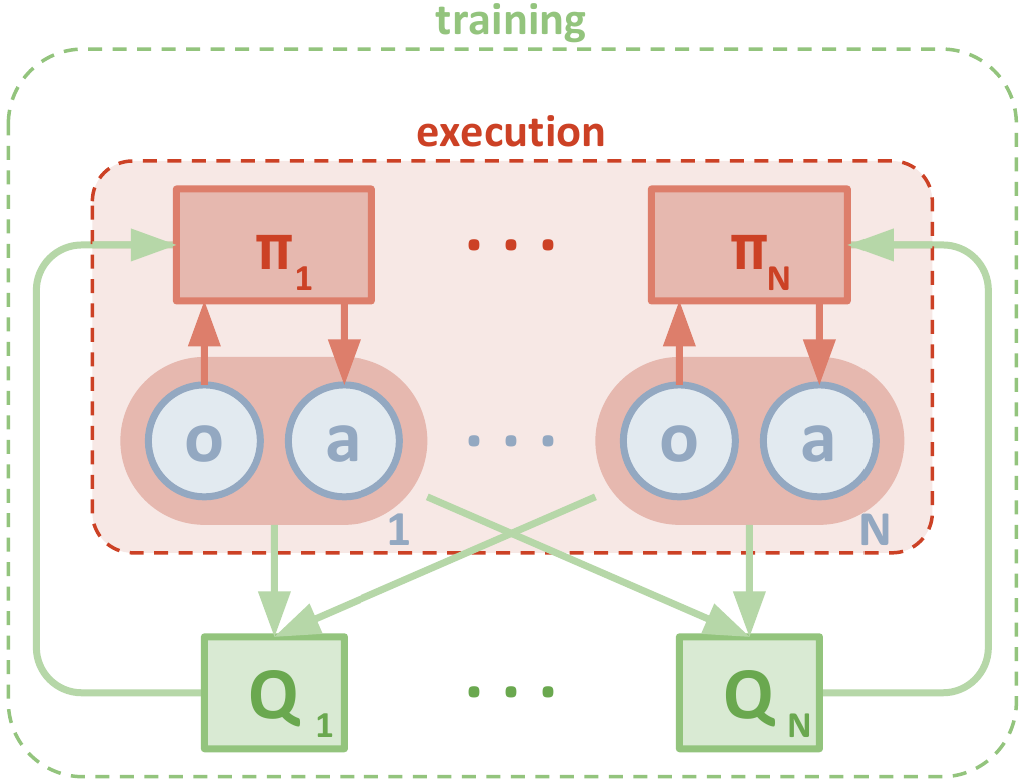
\includegraphics[width=0.48\linewidth]{Figures/MADRL/maddpg.png}
    \caption{The MADDPG architecture~\citep{Lowe2017_MADDPG} illustrating the centralised critics training decentralised policies. Each agent has a local policy used during training and execution, and a centralised critic, conditioned on the joint observation, used only during training.}
    \label{fig:MADDPG}
\end{figure}




\subsection{Value Factorisation}\label{sec:MADRL:ValueFac}

% Value factorisation concept
In Section~\ref{sec:MAL:CreditAssign}, we presented the multi-agent credit assignment problem that arises when multiple agents share a common reward signal and need a way to measure the contribution of their behaviour towards the observed common outcome. 
In such settings with a common reward signal, learning the value of local action $a^i$, with respect to the global return $G$ (as in Equation~\ref{eq:LocalValue}), can be problematic because $G$ does not depend only on $a^i$, but also on the other agents' actions. 
In Section~\ref{sec:MAL:CreditAssign}, we introduced methods that tackled this issue by computing a marginal contribution of each action. But, defining an effective marginal contribution can be tricky and computing it is usually expensive. 
Instead, another approach would be to learn the action-values of each action with respect to their real, unknown contribution, knowing that they are related in some way to the known common return. In other words, given the joint action-value $Q(\mathbf{h},\mathbf{a})$ estimating the expected global return (see Equation~\ref{eq:JointValue}) and local action-values $Q^i(h^i,a^i)\coloneqq\mathbb{E}_{\pi^i}[u^i\ |\ h^i,a^i]$, with $u^i$ the \textit{local utility} measuring the contribution of agent $i$ in $G$, we need to find how the local values compose the joint value:
\begin{equation}
    Q(\mathbf{h},\mathbf{a})=f(\{Q^i(h^i,a^i)\}_{1\leq i\leq n},\mathbf{h}).
\end{equation}
The function $f$ describes how each local value contributes to the joint value, depending on the joint history. Given the global return $G$, \textbf{value factorisation} (or "value decomposition") approaches learn the joint action-value and a way to decompose it into local action-values (i.e., function $f$). Value factorisation is a form of implicit credit assignment where we learn local value functions by learning how they compose the global value. 

% IGM property
Learning this properly allows having local action-value functions that can be used for choosing greedy local actions for each agent. Because the objective is to maximise the global return, this requires that greedy local actions lead to optimal joint actions. This has been referred to as the \textbf{individual-global-max} (IGM; \cite{Rashid2018_QMIX}) property, requiring that choosing the greedy joint action with respect to the joint action-value corresponds to choosing greedy local actions with respect to each local action-value, i.e.:
\begin{equation}
    \argmax_\mathbf{a}Q(\mathbf{h},\mathbf{a})=\{\argmax_{a^i}Q^i(h^i,a^i)\}_{1\leq i\leq n}. \label{eq:IGM}
\end{equation}
Respecting this property is essential to be able to use the learnt local action-values for local action selection. Thus, a multi-agent value-based learning algorithm that follows the IGM principle can fit into the CTDE paradigm, with decentralised local action-values used during execution, trained in a centralised manner with the help of a learnt joint action-value. 

% VDN
\cite{Sunehag2018_VDN} introduced this idea with their \textbf{value decomposition network} (VDN), making the simple assumption that local action-values should sum up to the joint action-value:
\begin{equation}
    Q(\mathbf{h},\mathbf{a})\approx\sum_{i=1}^nQ^i(h^i,a^i).\label{eq:VDN}
\end{equation}
With this assumption, $Q$ is differentiable with regard to each $Q^i$. Thus, VDN is able to learn individual action-values, parameterised as deep neural networks, from the DQN objective (see Equation~\ref{eq:DQN}) completely end-to-end. This linear version of value factorisation has the advantage of simplicity and being computationally lightweight, which allows excellent scalability. 

% QMIX
While this linear decomposition is intuitively logical and follows the IGM property, there is no guarantee that the true factorisation function $f$ is a linear transformation of local utilities. Therefore, the formulation of VDN limits the factorisation operation and the learnt representations of joint and local action-values. To address this, \textbf{QMIX}~\citep{Rashid2018_QMIX} introduces a separate "mixing" neural network that takes the local action-values and the global state as input, and outputs the joint action-value: $Q(s,\mathbf{a})=f_{MIX}(\{Q^i(h^i,a^i)\}_{1\leq i\leq n},s)$ (see Figure~\ref{fig:QMIX}). Note that, in their implementation, they consider that the global state $s$ is available, but it can be replaced by the joint observation of history if needed. The mixing network learns a factorisation function that depends on the current state of the environment, allowing much richer factorisation capacities. To ensure that the IGM is respected, the mixing of local values must be monotonic: if a local value increases, the joint value must increase too, i.e., $\frac{\partial f_{MIX}}{\partial Q^i}\geq 0$. This monotonic constraint is ensured by having the weights of the mixing network be positive. But, this constraint must be applied only for the local action-values, not for the state. To allow this, QMIX employs a hypernetwork~\citep{Ha2017_Hypernetworks}, which uses a separate MLP, conditioned on $s$ to generate the weights of the MLP used for factorising the local action values. The absolute value of the generated weights is taken to ensure the monotonic constraint described above. Using a hypernetwork allows to depend on the state in a non-monotonic way and to learn more complex dependencies between the action values and the state~\citep{Zhou2020_LICA}. 


% QMIX extensions
Many subsequent works have extended QMIX to improve its performance~\citep{Son2019_QTRAN, Rashid2020_WQMIX, Zhou2020_LICA, Yang2020_Qatten, Wang2021_QPLEX, Peng2021_FACMAC, Iqbal2021_REFIL, Hong2022_RethinkingIGM, Zhou2022_PAC, Sun2023_DFAC, Xu2023_DAVE}. The main issue is the monotonic constraint that limits the potential of QMIX for modelling some factorisation functions, which might induce poor performance in some scenarios. 
% WQMIX and QTRAN: To tackle this, some heuristics might be used to  
% QTRAN and WQMIX use heuristics to try to better fit the IGM property, but they are still based on approximations that do not guarantee exact consistency with IGM.
\citet{Yang2020_Qatten} reformulate the factorisation as a weighted sum that can be learnt with an attention mechanism. 
\citet{Zhou2020_LICA} and \citet{Peng2021_FACMAC} both extend QMIX to be used in an actor-critic algorithm. Having local policies for action-selection allows relaxing the monotonic constraint imposed in QMIX, required only because the local action-values were used for action-selection. Without this constraint, more accurate factorisation functions can be modelled. Additionally, using an actor-critic framework enables working with continuous actions~\citep{Peng2021_FACMAC} and learning stochastic policies~\citep{Zhou2020_LICA}. 
QPLEX~\citep{Wang2021_QPLEX} reformulates the problem by making the IGM property based on the advantage function instead of the action-value: given that $Q = V + A$ (as defined in Section~\ref{sec:DRL:DQN}) and that the action selection does not depend on V, the IGM constraint can be transferred onto the advantage function, rewriting Equation~\ref{eq:IGM} with the joint and individual advantages instead of action-values. This allows easier learning of a value factorisation. 
Finally, \citet{Sun2023_DFAC} propose a distributional extension of QMIX to better handle stochastic environments. 
While extensions provide several theoretical advantages, QMIX is still widely considered as state-of-the-art, and seen more often as a baseline. 
Also, it is interesting to note that the flexibility granted by QMIX for modelling more complex value factorisation might not be needed in many simpler tasks. In fact, VDN has been shown to outperform QMIX in some scenarios~\citep{Papoudakis2020_BenchmarkMADRL, Wang2021_UndestandValueFac}. 



\begin{figure}
    \centering
    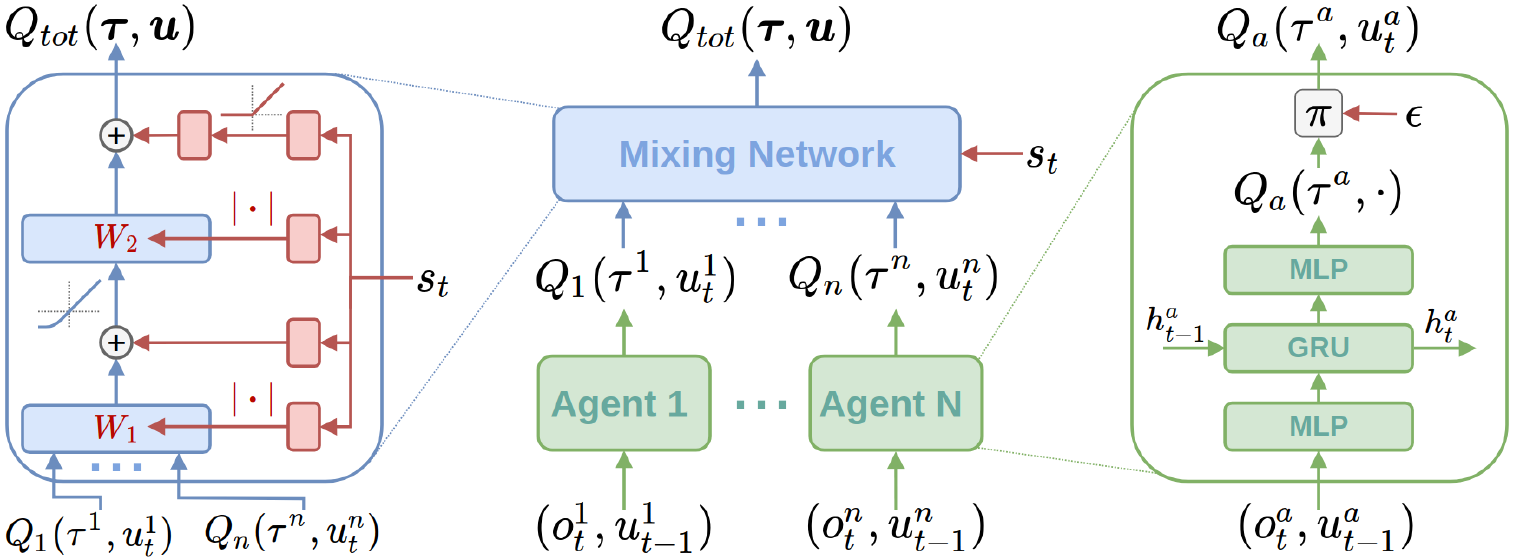
\includegraphics[width=0.8\linewidth]{Figures/MADRL/qmix.png}
    \caption{The architecture of QMIX~\citep{Rashid2018_QMIX} illustrating the learnt monotonic value factorisation. The middle shows the overall architecture with local action-value functions, mixed in to compute the joint action-value. On the left is shown the mixing network that takes in the local action-values to compute the joint action-value, with the weights generated by the hypernetwork (in red) conditioned on the global state. On the right, the architecture for a local action-value function is described, with a recurrent network (GRU) used for memory.}
    \label{fig:QMIX}
\end{figure}



\subsection{Differentiable Emergent Communication}\label{sec:MADRL:EmergentCommunication}

\begin{figure}
    \centering
    \begin{subfigure}[b]{0.88\textwidth}
        \centering
        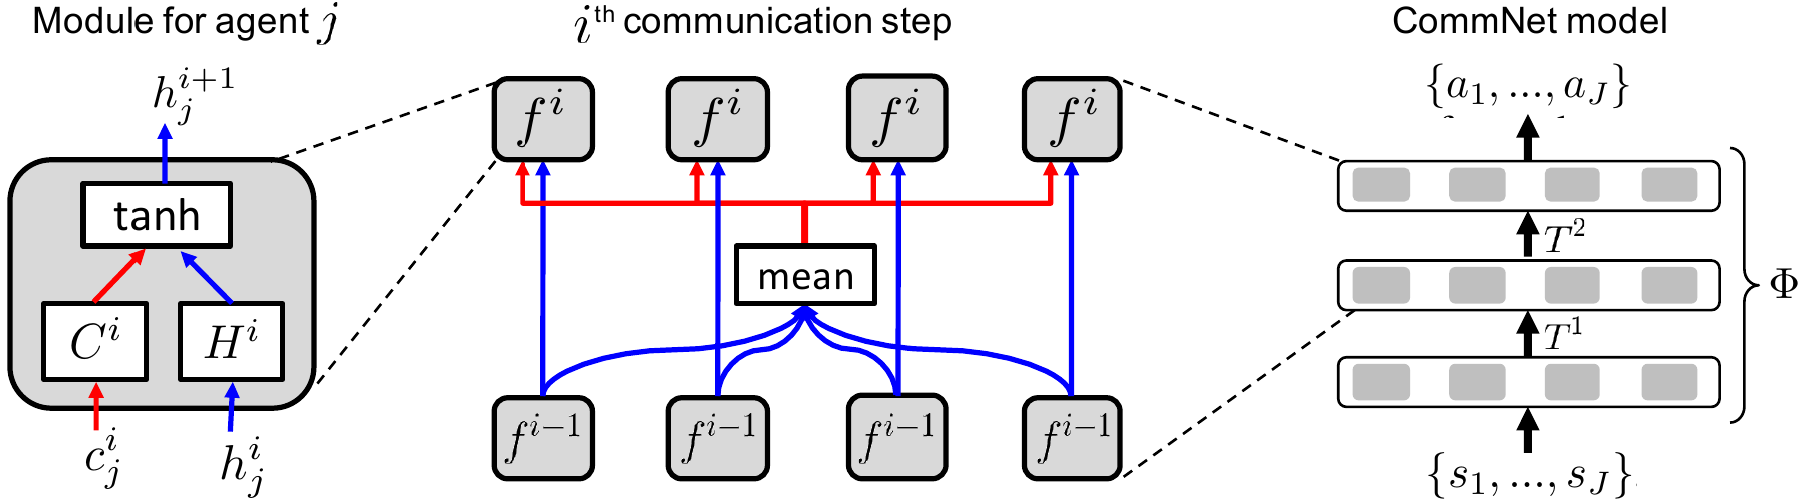
\includegraphics[width=\textwidth]{Figures/MADRL/commnet.png}
        \caption{CommNet~\citep{Sukhbaatar2016_CommNet}}
        \label{fig:CommNet}
    \end{subfigure}
    \begin{subfigure}[b]{0.52\textwidth}
        \centering
        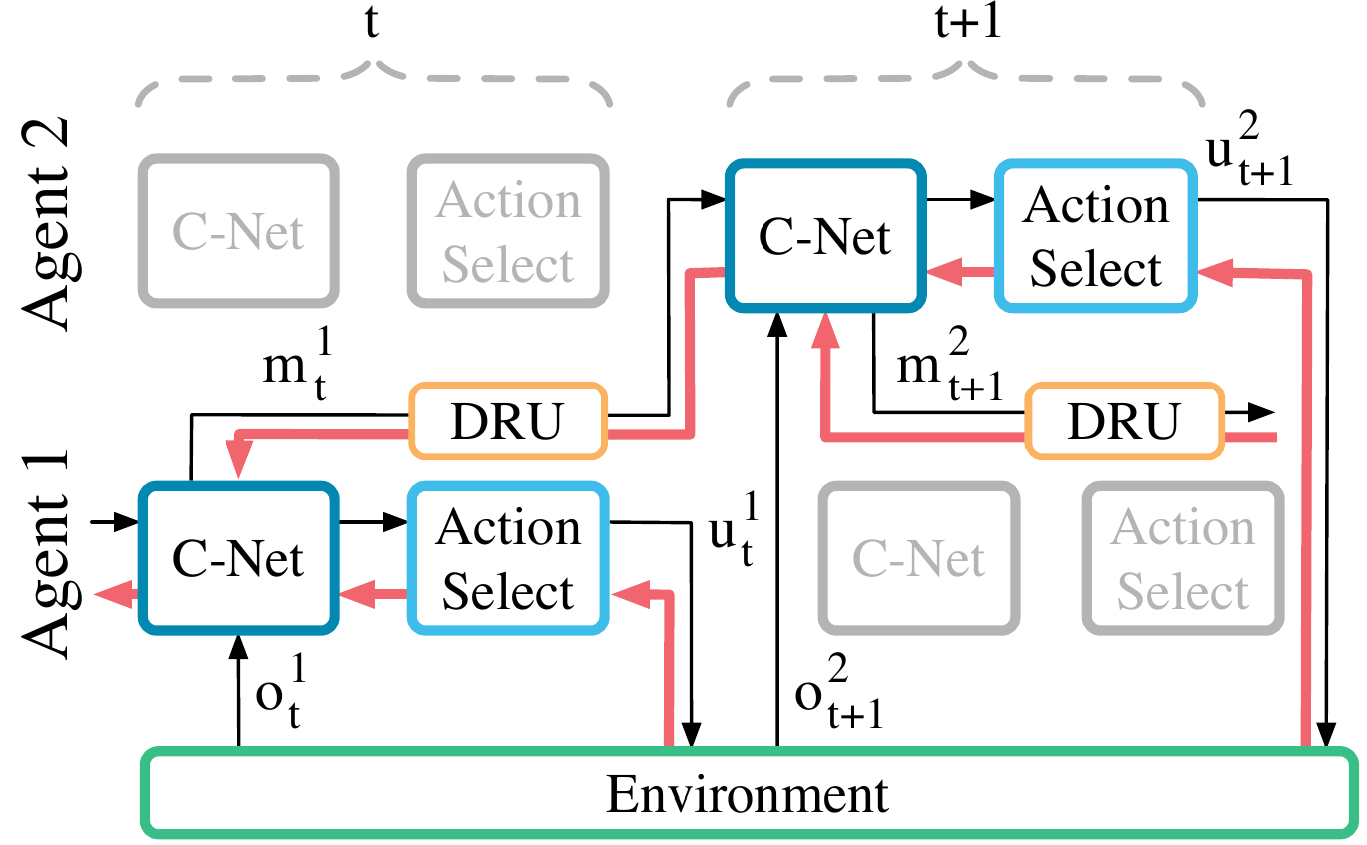
\includegraphics[width=\textwidth]{Figures/MADRL/dial.png}
        \caption{DIAL~\citep{Foerster2016_DIAL}}
        \label{fig:DIAL}
    \end{subfigure}
    \caption{Two architectures of differentiable communication. (a) CommNet learns a centralised communication network that shares local information in multiple rounds of communication before choosing local actions. (b) DIAL learns decentralised communication with centralised training, by allowing gradients to flow between agents. Because messages result from differentiable operations of neural networks, communication can emerge from back-propagation of gradients from the RL objective.}
\end{figure}

An important part of human interactions is communication. We often use our multi-modal communication abilities (e.g., speech, language, hand gestures, facial expressions) to share our knowledge, coordinate our actions, negotiate, or express goals and feelings. It is therefore natural to study communication in the context of multi-agent learning. We have seen, in Section~\ref{sec:MAL_issues}, that the decentralised aspect of multi-agent settings gives rise to many issues that can be alleviated with efficient multi-agent communication. To achieve this, agents need to learn how to communicate. This may be summarised as learning \textit{what to communicate} and \textit{how to communicate it}. A popular approach for learning communication in a multi-agent setting is to let agents develop their own communication system in the process of learning to complete a given task. This gives rise to an emergent communication system that specifically fills the communication needs of the task. 

% Differentiable communication
Recently, a successful approach to emergent communication with MADRL has been to implement communication as a differentiable sub-step of the action-selection process~\citep{Sukhbaatar2016_CommNet, Foerster2016_DIAL}. By using only differentiable operations -- i.e., neural networks -- to generate and process the messages, the gradients of the RL objective can be back-propagated through the message-generating modules so they participate in maximising future returns. Importantly, having differentiable messages allows for gradients to be passed between agents: as a message generated by agent $i$ will impact the choices made by agent $j$, agent $i$ can be trained to generate messages that maximise agent $j$'s returns. This way, the communication mechanisms emerge from the task requirements. CommNet~\citep{Sukhbaatar2016_CommNet} introduced a centralised approach of differentiable communication (see Figure~\ref{fig:CommNet}), with all agents sharing a communication network enabling information sharing and trained to maximise the joint return. DIAL~\citep{Foerster2016_DIAL} took this into the CTDE paradigm (see Figure~\ref{fig:DIAL}), with each agent's communication network (C-Net in the figure) trained from the other agent's learning objective. In these two approaches, neural networks generate differentiable messages comprised of a vector of continuous values, which may carry information to other agents. By learning to maximise the RL objective, the message-generating networks are trained to generate messages that allow other agents to select better actions. 

This approach of differentiable communication has been extended in various ways for more targeted information sharing~\citep{Hoshen2017_VAIN, Jiang2018_ATOC, Das2019_TarMAC} or to limit bandwidth usage~\citep{Singh2019_IC3Net, Zhang2019_VBC, Wang2020_IMAC, Han2023_MBC}. While previously cited works use \textit{continuous vectors} as messages, others have developed techniques to use \textit{discrete symbols} for communicating~\citep{Cao2018_Negotiation, Lazaridou2018_Emergence, Jaques2019_SocialInfluence, Kim2018_SchedNet, Rita2022_GenOverf}. Discrete symbols are advantageous because they limit the bandwidth of transmitted messages. They also incite the emergence of certain qualities of natural languages that make human communications so efficient~\citep{Mordatch2018_GroundedCompo, Chaabouni2019_AntiEfficient}. 

% problem with emergent comm, quick word on grounding and ref to chap 4
While emergent communication allows efficient learning of information transmission with deep RL, it has important limitations. As with all deep learning approaches, it acts as a black box that lacks practical ways of interpreting and measuring its efficiency~\citep{Lowe2019_Pitfalls, Lazaridou2020_DeepEmergentComm}. Because it emerges from task-oriented training in a closed group of agents, the resulting communication mechanism will be hardly usable for solving different tasks and communicating with other agents. For these reasons, methods are investigated to learn more interpretable and generalisable communication skills. In Chapter~\ref{ChapterComm}, we will look into communication and language more in depth, to see how multi-agent communication can be improved. 





\subsection{Agent Modelling}\label{sec:MADRL:AgentModelling}

% Modelling other agents
Previously presented approaches rely on learning policy and value functions to learn multi-agent behaviour. This model-free approach predominates in multi-agent learning because learning a model in a multi-agent setting is made extremely difficult by the fact that, from one agent's perspective, other agents contribute to the environment dynamics: the transition probability and reward function. 
One step towards solving this is to learn a model of other agents' policies, based on previous observations~\citep{Albrecht2018_AgentModellingReview}. 
% this is a kind of multi-agent model-based approach, that can enable better planning or solving multi-agent issues such a scredit assignment or non-statio
In fictitious play~\citep{Brown1951_FictitiousPlay,Robinson1951_FictitiousPlay, Fudenberg1995_FictitiousPlay, Hofbauer2002_FictitiousPlay}, each agent keeps track of action counts by other policies to compute potential action probabilities, then choosing an action accordingly. Recent deep RL techniques have been employed to improve fictitious play and allow its use in more complex, partially observable environments~\citep{Heinrich2016_NSFP, Strouse2021_FCP, Papoudakis2021_LIAM, Rahman2023_GPL, Jing2024_OfflineOpponentModel}. 
Bayesian learning goes further by tracking probabilities over possible policies for other agents, allowing to model uncertainty about their current reasoning~\citep{Jordan1991_Bayesian, Kalai1993_Rational, Bowling2001_Rational, Foerster2019_BAD, Hu2020_SAD}. 
Such agent modelling approaches are promising for learning intricate multi-agent interactions, as they allow to adapt to the observed behaviour of other agents instead of trying to learn a policy able to effectively answer to any situation. Additionally, this approach has the intuitive advantage of emulating the way human beings approach their interactions with other intelligent entities, as described by the \textit{theory of mind} literature~\citep{Apperly2011_Mindreaders, Heyes2014_MindReading, Aru2023_DeepLearningToM}. 

% conclusion -> agent modelling is interesting direction, as model-based RL, it can lead to interesting planning abilities and help solving multi-agent problem such as credit assignment or non-statio.

% Raileanu2018_SOM: predict other agents' goals to 
% LOLA uses it to reduce non-statio by considering how other agents will learn, in the learning update
% Kim2021_IS uses it for driving communication

%  ToM?
% LOLA? introduces opponent modelling into learning to reduce non-stationarity, the learning update takes into account the fact that other agents will also change their behaviour.

% - Instead of making decisions based only on expected returns and how they may be maximised by other agents, one could prefer explicetly predict the other agents goals and/or policies based on previous behaviours [Albrecht2018_AgentModellingReview].
% - Fictitious play (A128) [Brown1951_FictitiousPlay,Robinson1951_FictitiousPlay, Fudenberg1995_FictitiousPlay, Hofbauer2002_FictitiousPlay]
%   - Keeps track of action count by each policy to compute probability of each actions, and computes a best response to the modelled policies
%   - improvements with recent deep RL techniques allow to better learn agent models in more complex, partially observable environments [Heinrich2016_NSFP, Strouse2021_FCP, Papoudakis2021_LIAM, Rahman2023_GPL, Jing2024_OfflineOpponentModel]
% - Bayesian learning (A134): 
%   - track probabilities overs possibles policies for other agents, allowing to model the uncertainty of one agent's about the others' policies [Jordan1991_Bayesian,Kalai1993_Rational,Bowling2001_Rational, Foerster2019_BAD, Hu2020_SAD]
% (  - modelling uncertainty enables considering the value of gaining information about other agents when selecting actions [])
% - ? Theory of Mind

%   LOLA!

% REFS A127, Albrecht2018_AgentModelling





% -------------------------------------------------------------------------------------------------

\section{Robotic Perspectives on MADRL Research: Open Challenges and Shortcomings}\label{sec:MADRL_RobotPerspective}

One of the key objectives of MADRL research is to facilitate the integration of robots into our daily lives. The real world is inherently multi-agent, as almost all conceivable situations involve interactions with other intelligent entities. Consequently, MADRL research aims to extend RL algorithms to be applied in complex multi-agent settings that more accurately reflect everyday scenarios. However, despite this objective, the current state of research has not yet come this far. The methods presented in the previous section are hardly applicable to robotic settings without significant modifications. This is partly because these methods are designed to be general multi-agent learning approaches, rather than being specifically designed for robotics. However, it may also result from some inherent limitations in their learning techniques or shortcomings of MADRL research. 

In this section, we present four important challenges faced in MADRL research that must be addressed to enable the progress of MADRL algorithms in robotics. We define these challenges, examine how they are typically addressed, explore specific approaches to overcome them, and discuss potential improvements. While there may be other obstacles to overcome, we believe these challenges represent the main avenues for improving robotic control in complex multi-agent environments. 



\subsection{Benchmarking MADRL}\label{sec:MADRL:Benchmark}

% Many different environments
Rigorous evaluation and comparison of different MADRL methods have been difficult to carry out due to several key challenges. Firstly, there is a large variety of learning environments and tasks, with little consensus on which setting should be used for studying which multi-agent problem. The most frequently found environments are the \textbf{Starcraft multi-agent challenge} (SMAC, see Figure~\ref{fig:SMAC};~\cite{Samvelyan2019_SMAC}) and the \textbf{multi-agent particle environment} (MPE, see Figure~\ref{fig:MPE};~\cite{Lowe2017_MADDPG}), but many others are also studied (see Figures~\ref{fig:madrlenvs}c-f). Most environments have multiple tasks available for training and testing algorithms. But, it is often unclear what multi-agent learning problems are featured in a given task. Thus, different works choose different environments and tasks arbitrarily based on their preferences, available computing power, and the performance of their method. 
This complicates the comparison of different works that tackle different environments and tasks. Additionally, the value and rigour of these environments are seldom questioned, as shown by the recent revision of SMAC after it was found to be solvable by only observing the current time step~\citep{Ellis2023_SMACv2}. 
Some other interesting environments are often proposed, for more efficient computation~\citep{Lechner2023_GigaStep, Michalski2023_SMACLite}, human-agent teaming~\citep{Carroll2019_Overcooked}, for allowing more agents~\citep{Lechner2023_GigaStep}, more various tasks~\citep{Leroy2023_IMPMARL}, or more realistic settings~\citep{Kurach2020_GoogleFoot, Vinitsky2022_Nocturne}; but there are seldom included in new studies and benchmarks. 

% Implementations
Secondly, a thorough comparison with all existing methods is difficult. Learning multi-agent policies generally takes time and computing power. Among the available implementations, multiple versions of the same methods may have slight differences that are not always clearly stated. Different works might use different programming tools. While the programming language Python is widely adopted in Machine Learning, various Python libraries exist for implementing learning algorithms. No single library is universally preferred\footnote{Pytorch (\url{https://pytorch.org/}) is the most used in research, but some still use TensorFlow (\url{https://www.tensorflow.org/}), and a growing number of people prefer JAX for its computational efficiency~\citep{Jax2018}.}, leading to significant differences that prevent easy adaptation from one library to another. 

% In-method discrepancies
Lastly, the implementation of each method may differ from one work to another. All methods come with a very large set of hyperparameters, with some having a great impact on performance. Deep RL methods, which serve as the foundation for MADRL methods, can be implemented differently, with some implementation tricks having a major impact on performance. This variability makes comparison across different studies challenging.

% MADRL envs: SMAC, MPE, LBF, RWARE, Hanabi, magym
\begin{figure}
    \centering
    \begin{subfigure}[c]{0.35\textwidth}
        \centering
        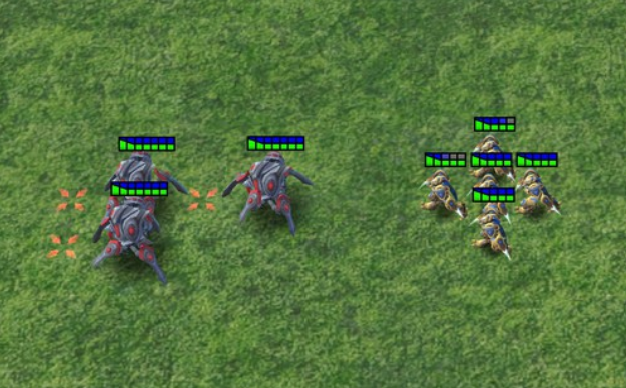
\includegraphics[width=\textwidth]{Figures/MADRL/smac.png}
        \caption{SMAC}
        \label{fig:SMAC}
    \end{subfigure}
    \hfill
    \begin{subfigure}[c]{0.24\textwidth}
        \centering
        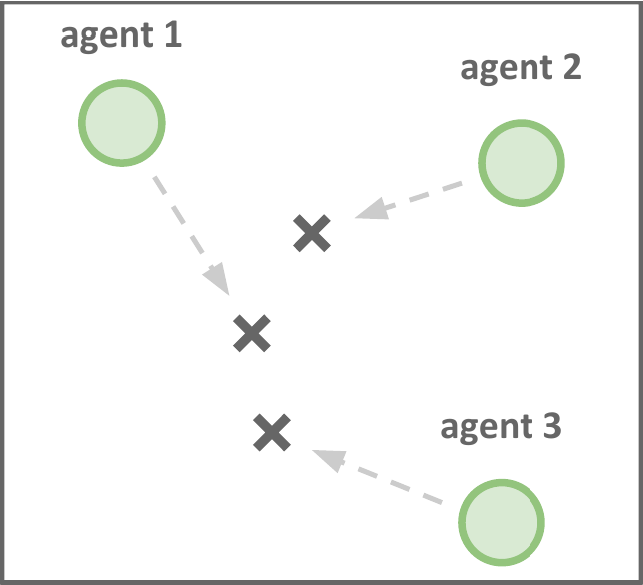
\includegraphics[width=\textwidth]{Figures/MADRL/mpe.png}
        \caption{MPE}
        \label{fig:MPE}
    \end{subfigure}
    \hfill
    \begin{subfigure}[c]{0.225\textwidth}
        \centering
        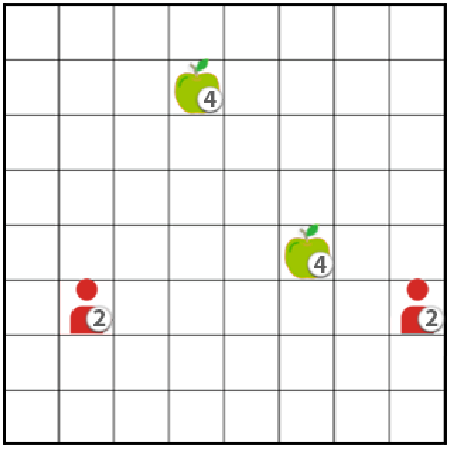
\includegraphics[width=\textwidth]{Figures/MADRL/lbf.png}
        \caption{LBF}
        \label{fig:LBF}
    \end{subfigure}
    
    \begin{subfigure}[c]{0.225\textwidth}
        \centering
        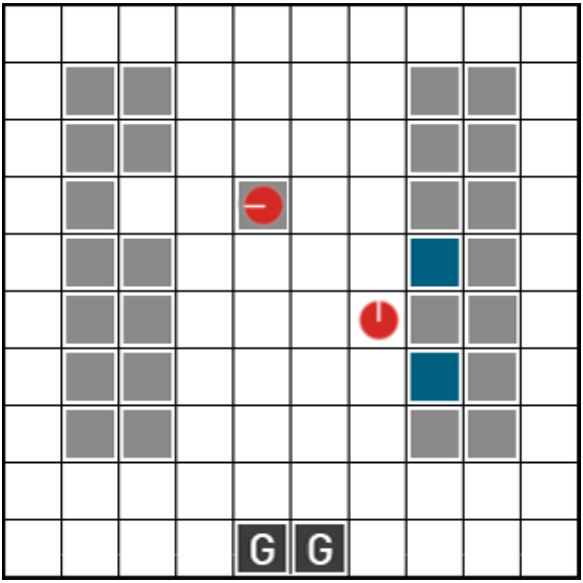
\includegraphics[width=\textwidth]{Figures/MADRL/rware.png}
        \caption{RWARE}
        \label{fig:RWARE}
    \end{subfigure}
    \hfill
    \begin{subfigure}[c]{0.44\textwidth}
        \centering
        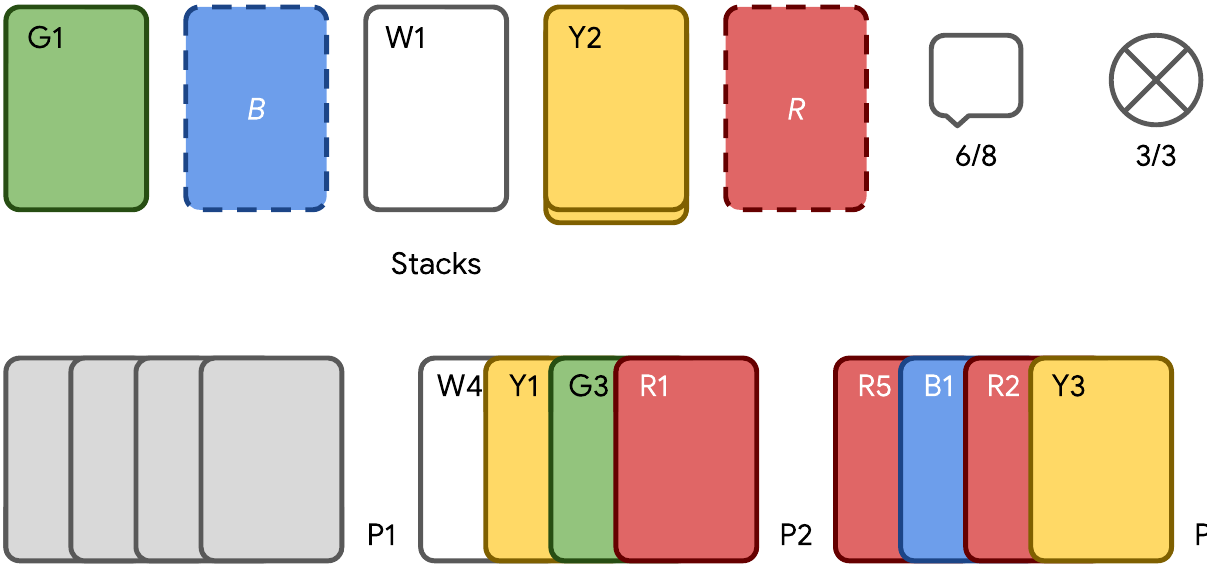
\includegraphics[width=\textwidth]{Figures/MADRL/hanabi.png}
        \caption{Hanabi}
        \label{fig:Hanabi}
    \end{subfigure}
    \hfill
    \begin{subfigure}[c]{0.225\textwidth}
        \centering
        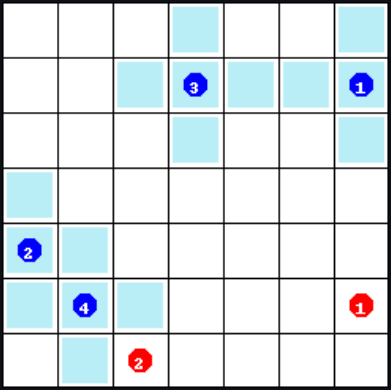
\includegraphics[width=\textwidth]{Figures/MADRL/magym.png}
        \caption{ma-gym}
        \label{fig:magym}
    \end{subfigure}
    \caption{The most used MADRL environments. (a) The \textit{Starcraft multi-agent challenge} (SMAC;~\cite{Samvelyan2019_SMAC}), with teams of units fighting opponents in various scenarios. (b) The \textit{multi-agent particle environment} (MPE;~\cite{Lowe2017_MADDPG}), a two-dimensional continuous environment with various tasks studying cooperative navigation and communication. (c) The \textit{level-based foraging} (LBF;~\cite{Albrecht2013_Foraging}) task, studying coordination in a grid world. (d) The \textit{multi-robot warehouse} (RWARE;~\cite{Christianos2020_SharedExp}), a robotic task in a grid world. (e) The cooperative card game \textit{Hanabi}~\citep{Bard2020_Hanabi} for studying complex team strategy learning and adaptation to teammates. (f) The \textit{ma-gym} two-dimensional grid world environment, with various cooperative tasks.}
    \label{fig:madrlenvs}
\end{figure}

% Benchmarking problem
For these reasons, assessing the progress of MADRL research is difficult. Performance reported in papers is hard to take at face value because of untold discrepancies hidden in the implementations and reported results~\citep{Singh2023_EvalMARL}. For example, \cite{Gorsane2022_BenchmarkCoopMARL} show inconsistencies in the performance of QMIX reported in different papers. The consequence of this lack of standardised benchmark is concerning: it is unclear which methods are the best for any given purpose, and therefore what method should be used as a baseline in any given setting. To advance learning in multi-robot environments, it would be difficult to determine the most valuable MADRL algorithms to use in these environments. 

% Existing benchmarks
Some benchmarks have been presented to try tackling this issue~\citep{Yu2021_Benchmark, Papoudakis2020_BenchmarkMADRL, Ellis2023_SMACv2, Bettini2023_BenchMARL}. They help clarify the field by providing a common ground for comparing important methods. However, there is limited variety in the environments used in these benchmarks, so the results might not hold in other tasks or more complex environments. It is also unclear what exact skill sets are required in each task, with only a rough measure of difficulty based on the returns obtained by all methods. This makes it difficult to discern the specific advantages of each method over others. Nevertheless, there are attempts to propose standardised evaluation protocols for new works~\citep{Gorsane2022_BenchmarkCoopMARL, Singh2023_EvalMARL}, which is a promising avenue for building stronger and more progressive research in MADRL. 

% Better benchmarks
To move forward, better practices should be adopted. Proposed methods should all disclose hyperparameters and specific code-level optimisations. Evaluation protocols and metrics should be standardised across all new publications~\citep{Gorsane2022_BenchmarkCoopMARL}. Benchmarks should include more diverse environments, integrating the wide range of potential learning problems studied across multi-agent learning: continuous and discrete settings, various degrees of centralisation allowed during training and execution, communication between agents, and different degrees of environmental complexity with environments closer to robotics. There is no doubt that MADRL research would immensely benefit from improving its evaluation protocols as such, allowing less biased comparison between methods and deeper analysis of their abilities. This is essential for efficiently advancing the field and ensuring that proposed methods are robust and generalisable across tasks and environments. 





\subsection{Exploration}

% The problem
Exploration is arguably one of the most important problems in single-agent RL~\citep{Hao2024_ExploReview}. It is particularly crucial when dealing with sparse rewards, where only a few interactions in the environment yield positive reinforcement signals. Such settings are often termed "hard-exploration" problems, requiring techniques allowing consistent discovery of the infrequent rewarding states.
In multi-agent RL, the problem is exacerbated. Performance depends on the joint behaviour of all agents, requiring exploration of the space of joint policies to identify the best approaches. Exploration becomes a multi-agent problem, especially when coordination is necessary, as agents need to explore different ways to act in unison. 
Exploration is also a major subject in robotic environments. Partial observability complicates the issue, as one environment state may be observed from many different perspectives. Moreover, the safety concerns are both a constraint and an expectation for exploration. When exploration is conducted on robots, it should only involve safe states to ensure that robots do not injure themselves or others~\citep{Koller2018_MBCSafeExp, Ding2021_SafeExp}. At the same time, exploration is a way to find the optimal strategies that are safer for the robots. In this sense, exploration might be conducted in simulation to identify safe behaviours to execute on physical robots~\citep{Garcia2015_SafeRL, Brunke2022_SafeLearningRobots}. 

% How methods explore
Most single and multi-agent RL approaches treat exploration arbitrarily by infusing randomness into the behavioural policy during training. Q-learning-based approaches employ the epsilon-greedy strategy (see Section~\ref{sec:RL:Qlearning}), policy-based approaches either add noise to actions, as seen in DDPG, or maximise the entropy of the policy, as in PPO (see Section~\ref{sec:DRL:Policy}). However, these methods are often insufficient for dealing with hard exploration problems~\citep{Ostrovski2017_PseudoCounts, Pathak2017_ICM, Burda2019_RND}. In multi-agent environments, random exploration often leads to the problem of relative overgeneralisation, where agents are attracted towards suboptimal Nash equilibria because the optimal strategy is too marginal to be found consistently through random exploration~\citep{Wiegand2003_RelOvergen}. 
In Chapter~\ref{ChapterJIM}, we will tackle this issue of multi-agent exploration by describing the problem of \textit{relative overgeneralisation} that results from poorly coordinated exploration, reviewing the related literature, and exploring intrinsic motivation to explicitly induce joint exploration. 




\subsection{Generalisation}\label{sec:MADRL:Generalisation}

Generalisation is a significant problem in machine learning and single-agent RL, concerning the robustness of learnt models to situations unseen during training. In RL, this may correspond to different initial conditions or new environmental settings. A good model is one that maintains its training performance in these new situations. In the multi-agent setting, the problem persists and even evolves with multiple agents, requiring to handle changes in the strategies of other agents. 

In machine learning, good generalisation is typically achieved through extensive training on very large amounts of data. However, this becomes challenging when faced with embodiment issues (see Section~\ref{sec:MAL:Embodiment}). In RL, the training data is generated by the agents themselves. Thus, in multi-agent RL, acquiring a comprehensive understanding of the joint policy space is a challenging exploration problem, as discussed in the previous section. In multi-agent RL, agents usually train in "self-play", with a fixed team of agents learning by trying to solve the task together. However, this often leads to agents converging to an arbitrary convention on collective behaviour, which may not hold with new partners. This is a problem in robotic settings, where the environment is dynamic and robots are expected to efficiently and safely handle new robotic or human partners. 

Generalising to new environmental situations can be facilitated by having diverse environmental settings, such as procedural maps, which allow training in many different scenarios and, hopefully, learning more general policies~\citep{Jaderberg2018_FTW, Cobbe2020_ProcGen}. For generalising to different partners, one approach is population-based training, involving a large number of agents trained in dynamic teams to face various strategies during training~\citep{Jaderberg2018_FTW, Liu2019_CoordThroughComp, Zhao2023_MaxEntropPop}. While this can be very effective~\citep{Jaderberg2018_FTW}, it requires extensive training sessions to converge to general strategies. This may be impractical in high-dimensional and dynamic robotic environments, where training is expensive and accounting for all possible modifications of a real environment is impossible. Moreover, if humans are involved, it is impossible to train for all possible changes in human behaviour. 

A promising approach is to learn to quickly adapt to any situation. In single-agent RL, \textit{zero-shot generalisation} methods aim to adapt to unseen environmental settings without being retrained~\citep{Kirk2023_ZeroShotGene, Haarnoja2024_Soccer}. In multi-agent RL, this concept extends to zero-shot, or \textit{ad hoc}, teaming, where agents are evaluated with new partners~\citep{Stone2010_AdHocTeam}. Agent modelling is promising for such settings, allowing to learn to model the "type" of policy observed in other agents~\citep{Strouse2021_FCP, Xie2021_LILI, Rahman2023_GPL, Yan2023_E3T}, or even the exact agents faced~\citep{Barrett2017_MakingFriends, Lanctot2023_RockPaperScissors}, allowing better reactions to the observed behaviour. If learned properly, zero-shot teaming can be a valuable tool for human-agent teaming. Training with humans is expensive, so it may be more efficient to learn to adapt quickly to any human partner~\citep{Strouse2021_FCP, Shih2021_ConventionsHumanAI, Xie2021_LILI, Yu2023_HiddenUtilitySP, Yan2023_E3T}. 



% \subsection{Decentralisation}

% while centralised methods were popular in earlier MARL research, recent research shifts to more decentralisation
% (as shown in figure ?)
% ctde is a step
% but training would also benefit from being more decentralised
% for scaling to larger number of agents. many robotic applications are not limited in the number of robots or other intelligent entities. ctde methods that use centralised observations during training
% for learning on robots, 
% for continuous learning 

% Human-robot interaction
\begin{figure}
    \centering
    \begin{subfigure}[c]{0.41\textwidth}
        \centering
        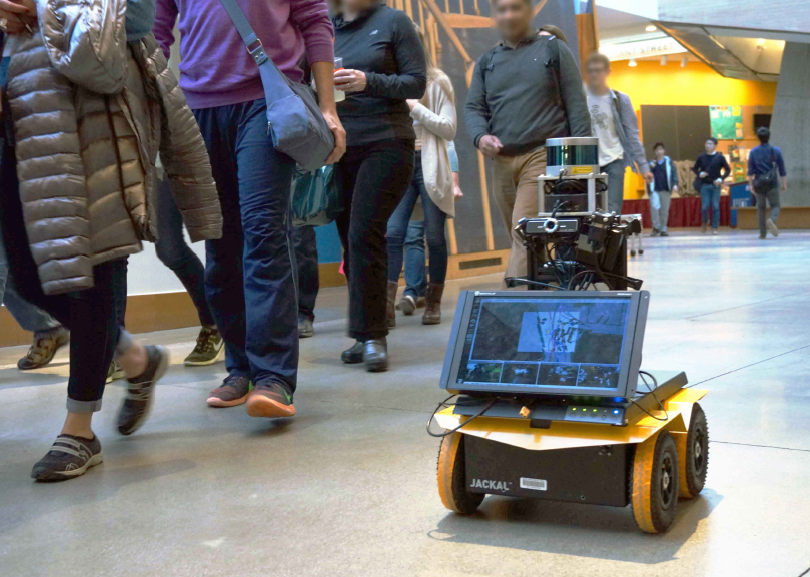
\includegraphics[width=\textwidth]{Figures/MADRL/robnav.png}
        \caption{}
        \label{fig:robnav}
    \end{subfigure}
    \hfill
    \begin{subfigure}[c]{0.39\textwidth}
        \centering
        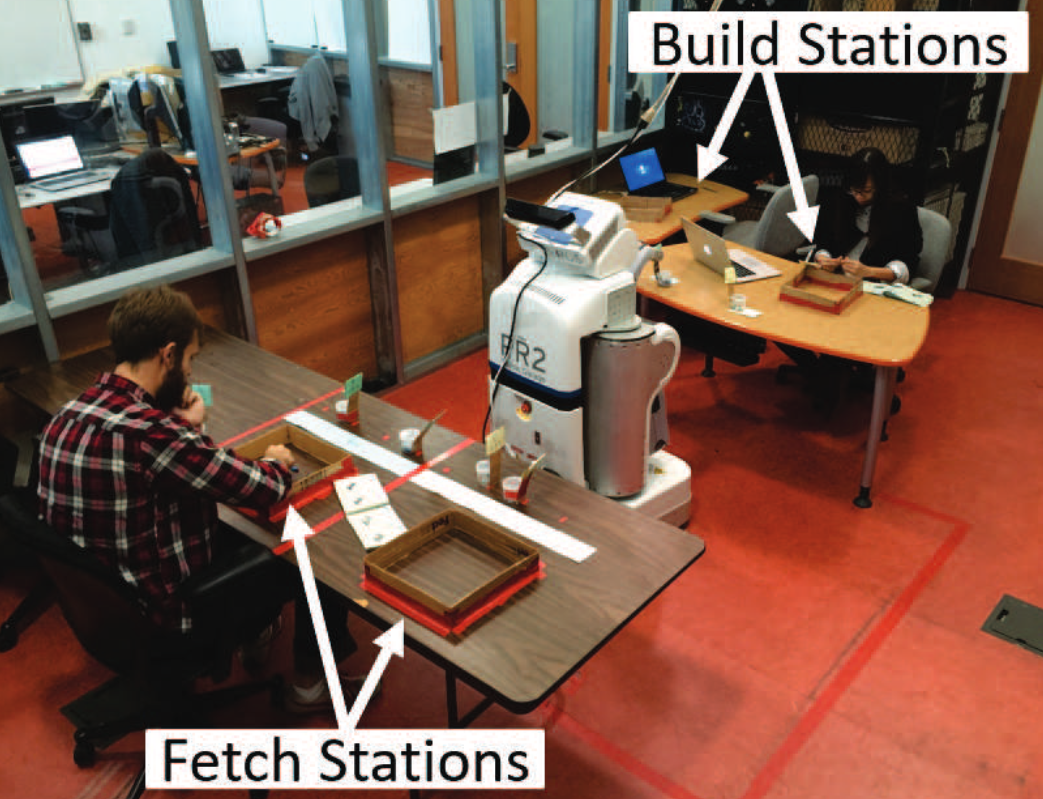
\includegraphics[width=\textwidth]{Figures/MADRL/robassist.png}
        \caption{}
        \label{fig:robassist}
    \end{subfigure}
    
    \begin{subfigure}[c]{0.36\textwidth}
        \centering
        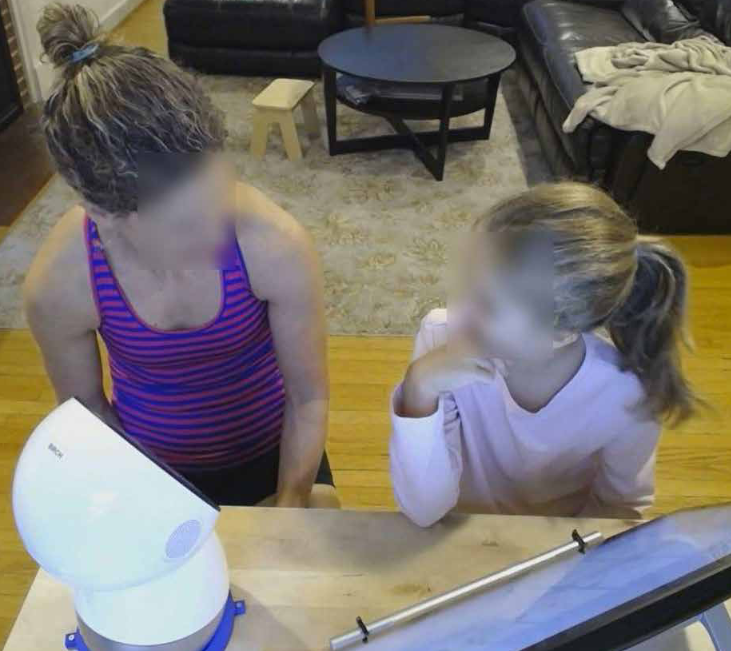
\includegraphics[width=\textwidth]{Figures/MADRL/robsocial.png}
        \caption{}
        \label{fig:robsocial}
    \end{subfigure}
    \caption{Examples of human-robot interaction. (a) Navigation of a robot in a human-populated environment~\citep{Chen2017_CollisionAvoidance}. (b) A robot assisting humans in a building task by fetching objects~\citep{Gombolay2017_MixedInitiative}. (c) A robot helping a child with autism spectrum disorder to learn social interaction~\citep{Scassellati2018_ASDRobot}.}
    \label{fig:HRI_examples}
\end{figure}

\subsection{Interaction}\label{sec:MADRL:Interaction}

Having robots in real environments implies the need for handling interactions with human beings. Figure \ref{fig:HRI_examples} shows different examples of human-robot interaction (HRI), illustrating various levels of HRI with differing degrees of connection between robots and humans, ranging from simply living in a human-populated environment to deep social interactions between robots and humans. Across all these potential scenarios, we can identify three sub-problems of HRI. First, to enable interaction between humans and computer systems in general, we need to understand how humans behave. This means studying how they go about solving a task, to know how robots could help them and how they should not~\citep{Shih2021_ConventionsHumanAI}. This means understanding how they interact with each other, to understand what makes a successful human interaction and how robots could be a part of them~\citep{Tseng2016_ServiceRobot}. This also means studying how humans react to robots when they interact with them, to understand the differences between human-human and human-robot interactions~\citep{Jung2020_TowerConstruct, Roesler2024_HumanRobotTrust}. And, this means studying how humans communicate with each other, investigating different tools like natural language, body language, and a large variety of social cues~\citep{Feine2019_SocialCues}. 
Analysing how humans behave in social interactions and when cooperating to fulfil a task can help design better robots and more effective learning approaches for HRI.

Second, HRI requires designing proper interfaces to enable smooth interactions. This involves physical interfaces, including the ability to sense, grasp, move, point and look at particular objects. These physical abilities are not needed only for interacting with human beings, but the HRI component might influence the design of these skills. Social interfaces are also required, with the help of human-like features such as voice, eyes, articulated faces, and gestures~\citep{Zlotowski2014_Anthropomorphism}. Being able to communicate with humans is also an important requirement to allow information sharing, teaching, strategy evaluation and correction~\citep{Mikolov2018_RoadmapMachineIntell, Crandall2018_CoopWithMachines}, and, more generally to bond more easily with artificial agents~\citep{Liu2022_ChildChatbotReading}. In Chapter~\ref{ChapterComm}, we will explore in greater depth the role of communication and language for human-agent interaction. 

Finally, HRI requires learning to behave around humans and cooperate with them. This is where MADRL research becomes relevant, as it enables learning in complex environments with multiple intelligent entities interacting. However, the main MADRL algorithms, discussed in Section~\ref{sec:MADRL_Review}, are not specifically intended for interacting with humans. They need to be extended using various techniques to efficiently address the problems linked with embodiment (see Section~\ref{sec:MAL:Embodiment}). The generalisation problem, described previously, must be tackled to enable robots to interact with any given human partner. And, to enable the use of MADRL algorithms on real robots, we need efficient approaches for bridging the reality gap (see Section~\ref{sec:MAL:RealityGap}). 





% -------------------------------------------------------------------------------------------------

\section{Conclusion}\label{sec:MADRL_Conclusion}

This chapter explored the domain of MADRL research, from the perspective of robotics. One of the objectives of MADRL research is to learn behavioural policies for controlling robots in the real world. Thus, it is important to reflect on the current state of progress in this domain, analyse the relevance of recent studies for robotics, and see how the challenges of robotic environments are addressed. After formally defining the tools of MADRL, we have presented the main challenges faced in multi-agent learning and robotics. Some of these challenges are specific to one of the two areas, but many overlap on many aspects. This analysis shows that connecting these two domains means dealing with many different forms of complexity, in environmental settings, interactions, and unpredictable situations. 

In Section~\ref{sec:MADRL_Review}, we presented a survey of the main avenues of MADRL research, describing how state-of-the-art methods learn policies in multi-agent settings. While some techniques have been shown to tackle increasingly complex tasks and environments, the main approaches are still far from being applicable in a robotic scenario without significant adaptation. This can be attributed to the fact that MADRL research is focused on the optimisation problem of multi-agent learning, i.e., finding an efficient multi-agent strategy. Doing so, it often overlooks some problems faced in realistic scenarios and thus fails to progress towards more efficient learning algorithms. 

In Section~\ref{sec:MADRL_RobotPerspective}, we introduced multiple challenges for MADRL research that should be addressed for improving the field, especially for moving towards robotic applications. The benchmarking issue faced in the domain is especially important to solve rapidly to ensure a more reliable research field and more steady progress. Next, the problems of exploration, generalisation, and interaction, are all key to improving the efficiency and applicability of new MADRL algorithms. We believe these challenges represent the main directions for advancing the control of robots in complex multi-agent environments, and that MADRL algorithms would benefit from investigating them further. 

Following this analysis of MADRL algorithms, in the next chapters, we propose two new methods for tackling some of the challenges defined previously. First, in Chapter~\ref{ChapterJIM}, we investigate the problem of exploration further, by highlighting the weaknesses of existing MADRL algorithms and proposing a method for improving them by exploring in a coordinated fashion. Next, in Chapter~\ref{ChapterComm}, we tackle the problem of communication in multi-agent systems, and propose an algorithm for learning to communicate with a pre-defined language which, as we demonstrate, serves multiple purposes of the robotic setting. 

\Chapter{Joint Intrinsic Motivation}{Inducing coordinated exploration in multi-agent environments.}

\label{ChapterJIM} 

\textit{This chapter extends the conference paper "}Joint Intrinsic Motivation for Coordinated Exploration in Multi-Agent Deep Reinforcement Learning\textit{", published in the Conference on Autonomous Agents and Multi-Agent Systems (AAMAS) 2024\footnote{Full paper available at: \url{https://arxiv.org/abs/2402.03972}}.}

% \vspace{4em}

\section{Introduction}


In Chapter~\ref{ChapterMADRL}, we reviewed the multi-agent deep reinforcement learning (MADRL) literature, its state-of-the-art approaches, and some important challenges that still need to be tackled for building better learning algorithms. 
One major issue in multi-agent learning is the problem of relative overgeneralisation~\citep{Wiegand2003_RelOvergen, Wei2016_RelOvergen} where agents struggle to find the optimal joint policy because local policies are attracted towards suboptimal areas of the search space. This makes most algorithms inefficient in tasks where the optimal strategy requires strong coordination among agents. Relative overgeneralisation can be described as a problem of exploration of the joint-observation space: as the success of the MAS depends on the coordination of multiple agents, exploring the joint-observation space is required to discover optimal joint behaviours. In this chapter, we address the question of how to explore the joint-state space to efficiently discover superior coordinated strategies for solving the task at hand. 

In single-agent RL, the problem of exploration has been studied to solve hard exploration tasks where positive reward signals are sparse. One solution is to use intrinsic motivation~\citep{Schmidhuber1991, Oudeyer2007_IntrMotiv, lehman2011abandoning} to incite agents to explore unknown parts of the environment. In addition to the environment reward, agents are given an auxiliary reward related to the novelty of encountered states. Maximising this intrinsic reward leads agents to visit previously unexplored regions of the environment, ultimately discovering new solutions to the task. These methods have shown great success in helping RL agents solve hard exploration tasks \citep{Pathak2017_ICM, Badia2020_NGU}. 

In the multi-agent setting, intrinsic objectives have also been studied to induce different kinds of behaviours in agents such as coordinated exploration \citep{Iqbal2019_MultiExplore}, social influence \citep{Jaques2019_SocialInfluence, Wang2020_EITI} or alignment with other agents' expectations \citep{Ma2022_ELIGN}. However, previous works have only used local observations to generate intrinsic rewards. With partial observability, local observations often lack crucial information to fully understand the current configuration of the environment. In the context of exploration, an intrinsic reward based only on local observations will lead to each agent exploring their own observation space, without considering the current state of other agents. This can result in inefficient exploration in cooperative tasks where the success of the MAS depends on the coordination of all agents.

In this chapter, we introduce a novel multi-agent exploration approach called \textbf{Joint Intrinsic Motivation} (JIM) which can be combined with any MADRL algorithm that follows the centralised training with decentralised execution (CTDE) para\-digm. JIM exploits centralised information during training to motivate agents to explore new coordinated behaviours. In order to compute joint novelty, JIM builds from two state-of-the-art single-agent intrinsic rewards: NovelD \citep{Zhang2021_NovelD} for exploring unknown parts of the environment, and E3B \citep{Henaff2022_E3B} for having more diverse trajectories. Adding this auxiliary reward to the agents' objective incites them to diversify their collective behaviour until they have a fair knowledge of the environment and can focus on the main task at hand. 

To demonstrate the advantages of our approach, we first design a simple test environment to showcase a clear example of relative overgeneralisation. We show that the state-of-the-art algorithm QMIX \citep{Rashid2018_QMIX} struggles in this scenario and that motivating the exploration of coordinated behaviour helps solve the task. Next, we validate these results in a continuous virtual environment, showing that coordination tasks benefit from joint exploration. Finally, further analysis is conducted to confirm the strength and scalability of our approach.






% -------------------------------------------------------------------------------------------------

\section{The Multi-Agent Exploration Problem}\label{sec:JIM:ExploProblem}

\subsection{Random Exploration Strategies}

% Random exploration strategies
To effectively learn with RL, algorithms need to balance an exploration-exploitation trade-off. Exploration of the environment is required to collect knowledge about the task. But, exploiting the learnt strategy allows focusing on parts of the environment that were discovered valuable, potentially making learning more efficient. 
Most RL methods tackle this issue by adding randomness in the agents' behaviour during training. Algorithms based on Q-learning use the $\epsilon$-greedy strategy, described in Section~\ref{sec:RL:Qlearning}, where agents start training by executing random actions and progressively shift to choosing actions only using the learnt action-value. 
In policy-based approaches, multiple exploration strategies are possible. 
In DDPG~\citep{Lillicrap2015_DDPG} and the multi-agent version MADDPG~\citep{Lowe2017_MADDPG}, exploration is performed by adding a Gaussian noise on the action generated by the deterministic formula: $a^i_t=\pi_i(o^i_t)+\epsilon$, with the noise $\epsilon\sim\mathcal{N}(0,\sigma)$ and $\sigma$ a hyperparameter controlling the standard variation of the exploration noise. 
In PPO~\citep{Schulman2017_PPO} and MAPPO~\citep{Yu2021_MAPPO}, because the policy is stochastic, actions can be drawn randomly from the generated action distribution during training: $a^i_t\sim\pi(.|o^i_t)$. In addition to this, exploration is also handled at the policy learning level, by maximising the entropy of the policy in the PPO objective (see Equation~\ref{eq:PPO-objective}). 
% (? Note that, because policies are independent in MADDPG and MAPPO, this means that exploration is done locally, which may induce non-stationarity?)

% Hard exploration problem in single-agent RL
All these approaches rely on randomness to ensure that agents gather essential knowledge about the environment and the task. However, in environments with very few positive reward signals, random exploration is not sufficient~\citep{Ostrovski2017_PseudoCounts, Pathak2017_ICM, Burda2019_RND}. In hard exploration problems, finding the positive reward signal requires specific sequences of hundreds of actions with no guidance. Discovering these trajectories by acting randomly is extremely unlikely. And, to be able to learn an efficient behaviour, RL algorithms require experiencing this behaviour many times, learning a little bit from each experience. Thus, random exploration is unlikely to enable efficient discovery and learning of optimal strategies in hard exploration problems. 





\subsection{Relative Overgeneralisation}\label{sec:JIM:RelOvergen}

% Relative overgeneralisation
\begin{figure}[t]
    \centering
    \begin{tabular}{c|c|c|c|}
        \multicolumn{1}{c}{} & \multicolumn{1}{c}{$A$}  & \multicolumn{1}{c}{$B$}  & \multicolumn{1}{c}{$C$} \\\cline{2-4}
        $A$ & $10$ & $-5$ & $-5$ \\\cline{2-4}
        $B$ & $-5$ & $7$ & $7$ \\\cline{2-4}
        $C$ & $-5$ & $7$ & $7$ \\\cline{2-4}
    \end{tabular}
    % \subcaptionbox{\label{fig:JIM:ro_map}}{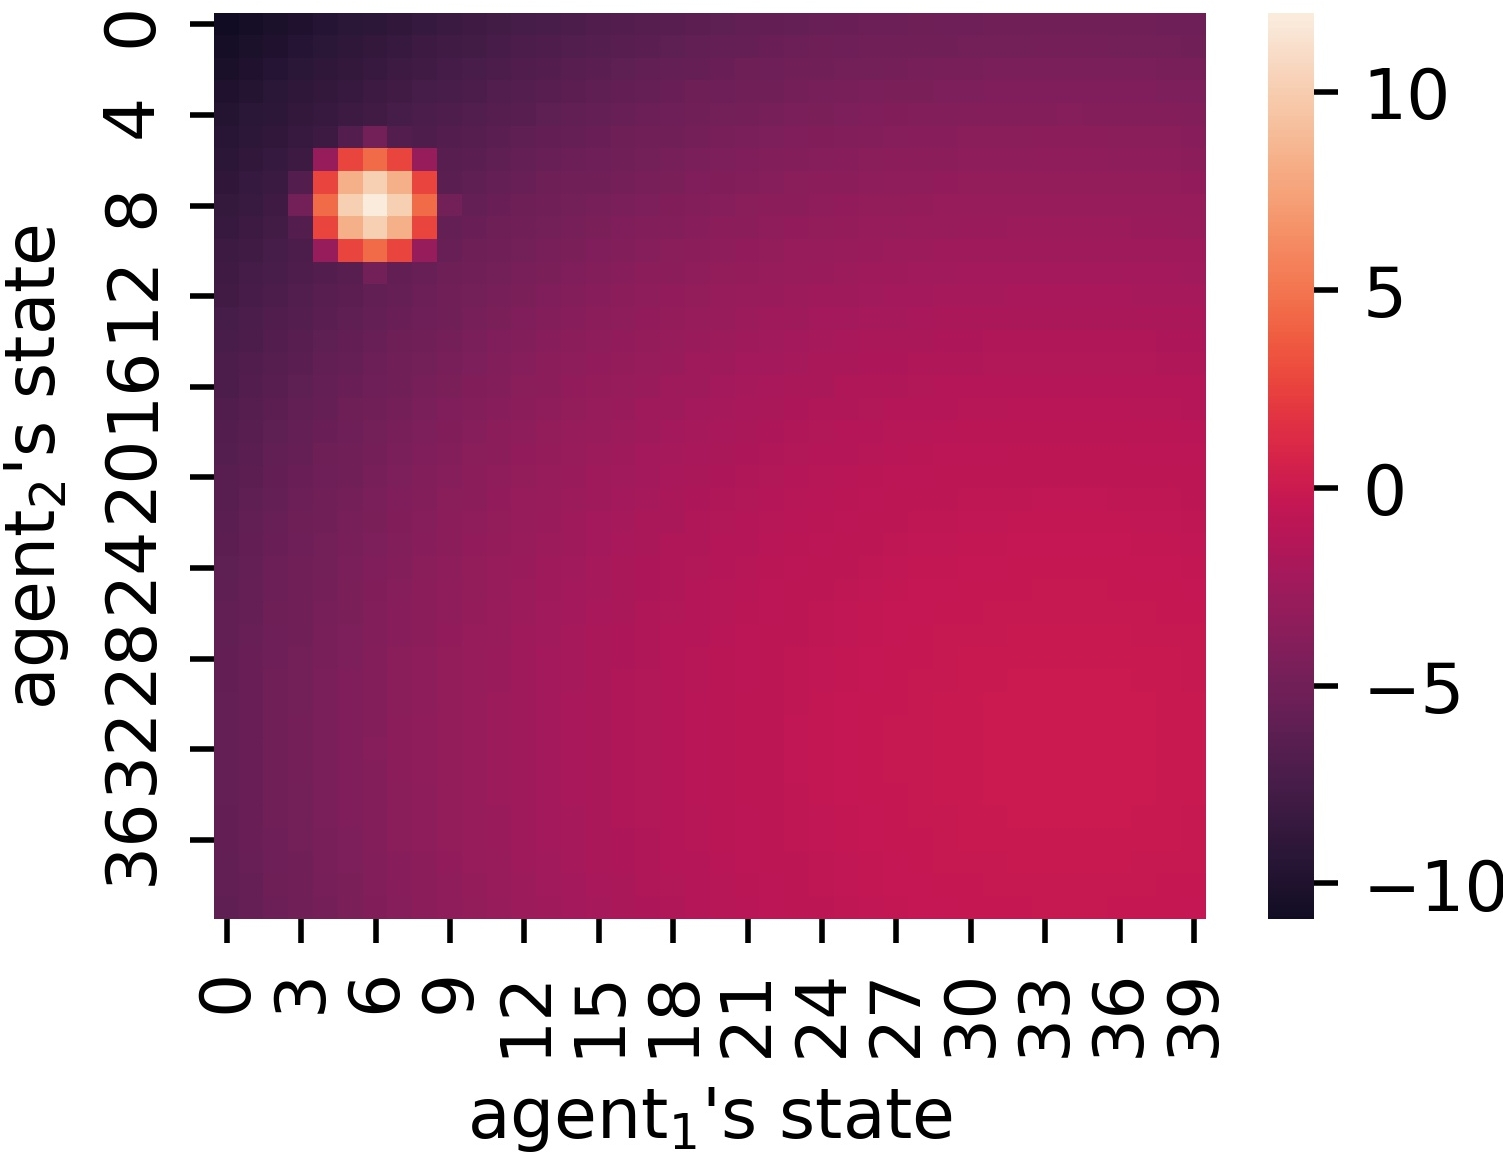
\includegraphics[width=0.45\textwidth]{Figures/JIM/ro_map30.jpg}}
    \caption{A social dilemma featuring the problem of relative overgeneralisation. Two agents have to choose between three actions. The optimal joint behaviour is both agents choosing action A. But, because actions B and C have a better average return when looked at locally, they will often be preferred.}
    \label{fig:JIM:ro_matrix}
\end{figure}

% Coordination is hard-exploration
The hard exploration problem becomes even worse in MAS as the completion of a task depends on the actions of multiple independent agents. In the context of MAS, a task that requires strong coordination between multiple agents can be considered a hard exploration problem. As defined in Section~\ref{sec:MAL:Coordination}, coordination requires the synchronisation of multiple agents' actions to achieve their common goal. Thus, a task requiring strong coordination is one where very few joint behaviours will produce the optimal returns. As in single-agent hard exploration problems, consistently discovering these optimal joint trajectories through random exploration will be extremely inefficient. 

In such cases, agents learning by randomly exploring their local state-action spaces will often struggle to find the optimal coordination strategy and settle for an easier suboptimal joint strategy. This is a problem known as \textbf{relative overgeneralisation}~\citep{Wiegand2003_RelOvergen, Wei2016_RelOvergen}, illustrated in Figure \ref{fig:JIM:ro_matrix}. In this example, there are two Nash equilibria: the optimal equilibrium with both agents choosing action A, and a suboptimal equilibrium where agents choose randomly between actions B and C with any probability. While the joint action (A, A) is clearly optimal, if agents explore their actions locally they will quickly find that actions B and C yield better returns on average. Only if all joint actions are explored and evaluated against each other, will the agents discover the optimal joint strategy. Thus, a joint-exploration approach can help solve the issue of relative overgeneralisation.







% -------------------------------------------------------------------------------------------------

\section{Explicit Exploration Strategies: Related Works}\label{sec:JIM:RelatedWorks}

% Faire une sous section pour :
% Exploration and Intrinsic rewards in single agent RL (parler de GoExplore, NGU, Agent57)
% Méthodes d'exploration multi plus poussées (hysteretic, leniency, MAVEN...)
% Intrinsic rewards in maRL

\subsection{Exploration in Single-Agent Reinforcement Learning}

To improve the exploration strategies of RL agents, multiple techniques have been employed. Inducing noise in learnt estimates can help RL agents having more diverse behaviour during training~\citep{Osband2016_BootstrappedDQN, Fortunato2018_NoisyDQN, Plappert2018_Noise, Osband2018_RandomizedValue, Chiappa2023_Lattice}. Hierarchical learning algorithms can be driven by the search for new skills, based on the idea that different skills generate different trajectories~\citep{Gregor2017_VIC, Eysenbach2019_DIAYN, Gehring2021_HierarchicalSkills}. Other works use a learnt model of the environment to plan exploration trajectories~\citep{Shyam2019_MAX, Sekar2020_Plan2Explore, Hu2023_PlanGoalExplore}. \cite{Ecoffet2021_GoExplore} achieve great results on hard exploration problems with a more handcrafted exploration method based on replaying past trajectories that resulted in unknown states, and starting exploring randomly from these states. Similarly, \cite{Pislar2022_WhenExplore} devise a strategy to decide when agents should explore with random actions based on their knowledge of the environment. 

However, the most successful approach for solving hard exploration problems has been inciting curiosity with intrinsic motivation. 
\textbf{Intrinsic motivation} is a technique for shaping the behaviour of RL agents by adding an auxiliary reward for them to maximise~\citep{Schmidhuber1991, Oudeyer2007_IntrMotiv, lehman2011abandoning}. This reward is computed by the agent, hence the name "intrinsic reward", based on its current state. Curiosity can be induced by computing a reward based on the novelty of the agent's trajectory. By learning to maximise this curiosity objective, the agent should learn to search for novel states. 
% In single-agent RL, curiosity has been defined to help agents solve hard exploration tasks~\citep{Schmidhuber1991,Oudeyer2007_IntrMotiv,lehman2011abandoning} by rewarding the visitation of states considered as novel. 
For measuring novelty, several methods use the error of trainable prediction models. The \textit{Intrinsic Curiosity Module} (ICM) \citep{Pathak2017_ICM} trains a model of environment dynamics and uses the prediction error as a measure of novelty. \textit{Random Network Distillation} (RND) \citep{Burda2019_RND} uses a neural network with fixed, randomly initialised parameters to produce a random encoding of the state, and trains a predictor network to generate the same encoding, the prediction error being the measure of novelty. With these two approaches, the prediction models will yield low novelty for states similar to what they have trained on, while producing high novelty for unknown parts of the environment. RIDE \citep{Raileanu2020_RIDE} and NovelD \citep{Zhang2021_NovelD} use respectively ICM and RND to compute a reward from the difference of novelty between the next state and the current state, pushing the agents to always seek novel states. Similarly, NGU \citep{Badia2020_NGU} and E3B \citep{Henaff2022_E3B} use clustering techniques to reward states that are distant from previously observed states. Agent57~\citep{Badia2020_Agent57} manages to solve the hard exploration games in the Atari benchmark by extending NGU to learn two value functions: one for the extrinsic reward and one for the intrinsic one; and by learning a meta-controller that decides whether to explore or exploit during training. Finally, AGAC \citep{FletBerliac2021_AGAC} trains an adversarial policy to predict the main policy’s output, the latter being rewarded with the former’s prediction error. 
%In our case, we choose to combine NovelD and E3B for their performance and simplicity.



\subsection{Exploration in Multi-Agent Reinforcement Learning}

% Leniency, hysteretic, MAVEN

To address the problem of relative overgeneralisation, better exploration strategies must be implemented in MADRL algorithms. Not all single-agent exploration strategies can be used efficiently in multi-agent settings. The noise-inducing approach could be another source of non-stationarity in a multi-agent algorithm. Also, plan\-ning-based techniques are not usable as learning a model in a multi-agent setting is challenging. However, some other approaches have been successfully pursued. 
MAVEN \citep{Mahajan2019_MAVEN} extends QMIX with a hierarchical policy that chooses goals common to all agents, and then explores the space of these joint goals to try different joint behaviours. 
Similarly, CMAE~\citep{Liu2021_CMAE} have agents sharing common goals, defined as states to reach, and use a curriculum approach for choosing joint goals of increased difficulty based on the number of times each goal-state has been experienced. 
\cite{Lupu2021_TrajeDi} promote policy diversity by learning a population of agents and maximising the divergence of each policy with regards to the rest of the population, which is shown to help agents be more versatile. 
Finally, EMAX~\citep{Schafer2023_EMAX} learn multiple joint value functions at once and explore by maximising the disagreement of the ensemble of joint values. 
% MAVEN 
% MultiSoftQ maximise the entropy of local policies in a MADDPG-style architecture
% Liu2021_CMAE learns to achieve subgoals that are gradually more diverse
% Schafer2023_EMAX learn an ensemble of joint value functions and drive exploration by rewarding agent locally with the disagreement of the ensemble of value

\subsection{Multi-Agent Intrinsic Motivation}

In MASs, there is a large variety of different ways to complete tasks, interact with teammates, and handle opponents. Different definitions of intrinsic motivation can stimulate the emergence of different types of behaviour. 
Social influence has been shown to help learn interesting multi-agent behaviour~\citep{Jaques2019_SocialInfluence, Wang2020_EITI}, by rewarding actions that have a significant impact on other agents. Learning to influence other agents helps train agents that actively look for interactions, thus avoiding lazy agents, and that try new behaviours during training, helping the exploration of joint behaviours. \cite{Ma2022_ELIGN} propose an intrinsic reward based on the average alignment with other agents' expectations. Depending on how this alignment reward is used, as a bonus or a penalty, this can promote more predictable or more surprising behaviours. 

Curiosity has also been studied for multi-agent exploration. ~\cite{Iqbal2019_MultiExplore} propose an approach for coordinated exploration using several metrics for estimating the novelty of observations that depend on all agents' past experiences. \cite{Zheng2021_EMC} extend VDN with a separate network that predicts local action-values, with an intrinsic curiosity reward based on the prediction error of these separate values. Finally, in a concurrent work, COIN~\citep{Li2023_COIN} proposed an intrinsic reward inspired by ICM that measures the novelty of the joint trajectories. Apart from COIN, other multi-agent intrinsic rewards use local observations for computing their intrinsic rewards. As shown in Section~\ref{sec:JIM:RelOvergen}, local exploration is not sufficient for exploring coordinated behaviours. Therefore, in the following sections, we present an approach for exploring the space of joint observations with an intrinsic reward inspired by recent works in single-agent curiosity. 








% -------------------------------------------------------------------------------------------------

\section{Background on Intrinsic Reward Definitions}\label{sec:JIM:IntrRew}


% Faire de chaque paragraph une sous section et étendre un peu si possible?


In Section \ref{sec:JIM:RelatedWorks}, we introduced intrinsic motivation as a way to incite agents to actively explore their environment. To this end, at each time step $t$, agents receive an augmented reward $r_t=r^{\text{ext}}_t+\beta r^{\text{int}}_t$, where $r^{\text{ext}}_t$ is the extrinsic reward given by the environment, $r^{\text{int}}_t$ is the intrinsic reward, and $\beta$ is a hyperparameter controlling the weight of the intrinsic reward in the agents' objective. We describe three methods of intrinsic motivation from the literature that we will use later in Section~\ref{sec:JIM:Algo}. 




\subsection{Random Network Distillation (RND)}\label{sec:JIM:RND}

In \textit{random network distillation} (RND), \cite{Burda2019_RND} compute novelty using two neural networks with the same architecture: a target network $\phi$ and a predictor network $\phi'$. The target's parameters are initialised randomly and fixed. It takes as input the state $s_t$ and produces a random embedding $\phi(s_t)$. The predictor is trained to output the same embedding, minimising the Euclidean distance:
\begin{equation}\label{eq:JIM:RND}
    RND(s_t)=\lVert\phi(s_t)-\phi'(s_t)\rVert_2.
\end{equation}
By training the predictor network to produce the same embeddings as the one generated by the target, the algorithm essentially tries to copy the parameters of the target in the predictor, or "distil" them. This distance $RND(s_t)$ is also used as a measure of the novelty of state $s_t$ and is given as an intrinsic reward to the agent. By training the predictor network along the agent, the predictor will get better at predicting the embeddings of states that are often seen by the agent during its trials. Thus, to accumulate more intrinsic reward, the agent will have to discover new states. 




\subsection{Novelty Diversity (NovelD)} \label{sec:JIM:NovelD}

Zhang et al.~\citep{Zhang2021_NovelD} build upon RND to devise a novelty criterion termed \textit{NovelD}, for "novelty diversity". It is defined as follows:
\begin{equation}\label{eq:JIM:NovelD}
    N(s_t, s_{t+1}) = \mathrm{max}[RND(s_{t+1}) - \alpha RND(s_t), 0]\times\mathds{1}\{N_e(s_{t+1})=1\},
\end{equation}
with $\alpha$ a scaling factor, $N_e$ an episodic count of visited states, and $\mathds{1}\{\cdot\}$ the indicator function that outputs $1$ if the condition is true. The first part is the core of the novelty criterion. It uses RND to reward agents for positive gains in novelty between the current and the next states. Thus, NovelD rewards the agent for always going towards newer states. The second part is an episodic restriction that ensures the reward is given only when state $s_{t+1}$ is observed for the first time in this episode. This ensures that agents cannot exploit one particularly novel state by staying in it. However, because this restriction is based on an explicit count of the occurrence of states during the episode, it limits the use of NovelD to discrete state spaces, as continuous states will likely never be reached more than once. 



\subsection{Exploration via Elliptical Episodic Bonuses (E3B)}\label{sec:JIM:E3B}

\cite{Henaff2022_E3B} propose \textit{exploration via elliptical episodic bonuses} (E3B), an episodic bonus based on the position of the observed state with respect to an ellipse that fits all states previously encountered in the current episode. Formally, it is computed as follows:
\begin{equation}\label{eq:JIM:E3B}
    b(s_t)=\psi(s_t)^\top C^{-1}_{t-1}\psi(s_t),
\end{equation}
with
\begin{equation}
    C_{t-1}=\sum_{i=1}^{t-1}\psi(s_i)\psi(s_i)^\top+\lambda I,
\end{equation}
where $I$ is the identity matrix and $\lambda$ a scalar coefficient. $\psi$ is an embedding network trained using an inverse dynamics model \citep{Pathak2017_ICM}: embeddings of following states $\psi(s_t)$ and $\psi(s_{t+1})$ are used by a separate neural network trained to predict the action $a_t$ taken between these states. As a result of this training process, $\psi$ encodes parts of the observation that are controllable by the agents (see the original paper for more detail,~\cite{Henaff2022_E3B}). Intuitively, $b$ can be understood as a generalisation of a count-based episodic bonus for a continuous state space. States that are close to previously encountered states in the current episode will yield low bonuses, whereas states that are very different will produce high bonuses. This incites the agent to have diverse trajectories. 







% -------------------------------------------------------------------------------------------------


\section{Joint Intrinsic Motivation Algorithm}\label{sec:JIM:Algo}

In this section, we introduce the Joint Intrinsic Motivation (JIM) exploration criterion for coordinated multi-agent exploration. We take inspiration from state-of-the-art intrinsic motivation techniques developed for single-agent RL and propose a new method for efficient multi-agent exploration. 
First, we define the main components of the intrinsic reward. Then, we explain how it is used in a multi-agent setting for exploring the space of joint observations. 


\subsection{Double-timescale Intrinsic Reward}\label{sec:JIM:DoubleTimeReward}

Similarly to previous works on single-agent intrinsic motivation~\citep{Badia2020_NGU}, we define a novelty metric that combines two exploration criteria working at different timescales:
\begin{itemize}
    \item A \textbf{life-long exploration criterion (LLEC)} that captures how novel is the current observation with respect to all observations since the beginning of training.
    \item An \textbf{episodic exploration criterion (EEC)} that captures the difference between the current observation and all previous observations in the current episode. 
\end{itemize}
Intuitively, the \textit{life-long reward} motivates agents to search for never-experienced parts of the environment. Meanwhile, the \textit{episodic bonus} induces more diverse trajectories. These two elements will work together to reinforce agents to efficiently explore their environment. 

We first define this intrinsic reward as it would be in a single-agent case, measuring the novelty of an agent's state. For each transition from state $s_t$ to the next state $s_{t+1}$, we define the double-timescale intrinsic reward as follows: 
\begin{equation}\label{eq:JIM:IntrRew}
    r_t(s_t, s_{t+1}) = N_{LLEC}(s_t,s_{t+1})\times N_{EEC}(s_{t+1}),
\end{equation}
with the life-long novelty $N_{LLEC}$ inspired from NovelD~\citep{Zhang2021_NovelD} (see Eq.~\eqref{eq:JIM:NovelD}):
\begin{equation}\label{eq:JIM:LLEC}
    N_{LLEC}(s_t, s_{t+1}) = \mathrm{max}[RND(s_{t+1}) - \alpha RND(s_t), 0],
\end{equation}
with $\alpha$ a scaling factor and $RND$ the novelty measure (see Eq.~\eqref{eq:JIM:RND}). Further, the episodic novelty $N_{EEC}$ uses the bonus from E3B~\citep{Henaff2022_E3B} (see Eq.~\eqref{eq:JIM:E3B}):
\begin{equation}\label{eq:JIM:EEC}
    N_{EEC}(s_{t+1}) = \sqrt{2b(s_{t+1})}.
\end{equation}

We make two modifications compared to previous works. First, we modify NovelD by removing the count-based episodic restriction that was limited to discrete state spaces. We replace it with the elliptical episodic bonus $b$ from E3B~\citep{Henaff2022_E3B}. This bonus acts as an episodic restriction by scaling $N_{LLEC}$ up or down, depending on the novelty of the current state compared to what has been observed during the current episode. Second, we take $\sqrt{2b(s_{t+1})}$ instead of simply $b$ to smooth the values given by this bonus, increasing the small ones and decreasing the large ones. This is because we observed that, in continuous state spaces (which was not studied in the original E3B paper), $b$ yielded extremely high bonuses at the start of the episode and quickly dropped to low bonuses after this. Thus, the smoothing function allows having a more controlled range of bonuses. 

Combining these two rewards makes it possible to take the benefits of both. $N_{LLEC}$ pushes agents to explore regions of the state space that are not well-known to agents, considering states observed since the beginning of training. Meanwhile, $N_{EEC}$ favours diverse trajectories, inciting agents to always seek new observations during a single episode. As the agents explore their environment, the prediction error of RND (see Eq.~\eqref{eq:JIM:RND}) slowly decreases. Thus, $N_{LLEC}$ decreases as well, tending toward zero. This allows to naturally shift from high exploration at the beginning of training, to progressively focusing on the extrinsic reward. Finally, as the episodic restriction does not rely on any explicit count of visited states, it can be used in continuous state spaces. 




\subsection{The Joint Intrinsic Motivation Algorithm}

\begin{figure}[h]
    \centering
    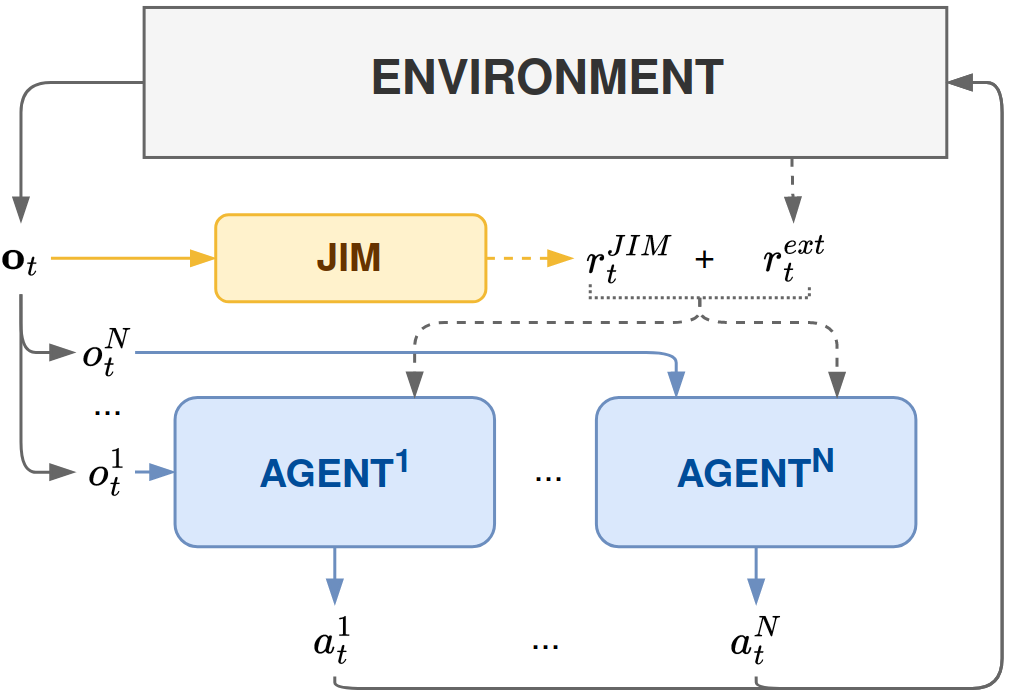
\includegraphics[width=0.6\textwidth]{Figures/JIM/archi_jim.png}
    \caption{Architecture for the Joint Intrinsic Motivation (JIM) algorithm. JIM has only one intrinsic motivation module for the whole multi-agent system, computing novelty of the joint observation $\mathbf{o}_t$. However, agents only use their local observation to choose their actions.}
    \label{fig:JIM:archi}
\end{figure}

Building from the intrinsic reward introduced previously, we propose the \textbf{Joint Intrinsic Motivation} (JIM) algorithm to incite MADRL agents to explore the joint-observation space. At each time step, all agents receive the same global reward $r_t=r^{\text{ext}}_t+\beta r^{JIM}_t$, where $r^{\text{ext}}_t$ is the extrinsic reward given by the environment, $r^{JIM}_t$ is our joint exploration criterion, and $\beta$ is a hyperparameter controlling the weight of the intrinsic reward. The exploration criterion in JIM uses the double-timescale intrinsic reward defined previously to compute the novelty of the joint observation:
\begin{equation}\label{eq:JIM:JIM}
    r_t^{JIM}(\mathbf{o}_t,\mathbf{o}_{t+1})=N_{LLEC}(\mathbf{o}_t,\mathbf{o}_{t+1})\times N_{EEC}(\mathbf{o}_{t+1}),
\end{equation}
where $\mathbf{o}_t=\{o_t^i\}_{0\leq i\leq N}$, i.e., the concatenation of all local observations. Figure \ref{fig:JIM:archi} shows the architecture for JIM. Compared to a local method that would use one intrinsic motivation module per agent, JIM computes only one intrinsic reward. This makes it possible to capture novelty at the team level, rather than at the individual level only, while requiring fewer parameters and less computation. As agents are rewarded by the novelty of the joint observation, they will learn to search for new combinations of observations with other agents of the system, rather than only exploring their local-observation space. This will induce the exploration of new configurations of the environment and thus help find better coordinated strategies.

As JIM uses joint observations for computing the intrinsic reward, it can be associated with any MADRL algorithm that fits in the CTDE paradigm. These algorithms usually employ a centralised value function \citep{Lowe2017_MADDPG,Rashid2018_QMIX,Yu2021_MAPPO} that looks at the joint observation to predict the value of the agents' actions. Such centralised value functions will be able to associate rewards provided by JIM to new configurations in the joint observation space, thus inducing agents to actively search for these configurations. 

One could note that the joint observation has two notable drawbacks: the number of dimensions grows linearly with the number of agents and there is a risk of capturing redundant information. These issues are both alleviated by using embedding networks to encode the joint observation into a more condensed latent representation. Both $N_{LLEC}$ and $N_{EEC}$ use embedding networks, respectively $\phi$ and $\psi$ (as described in Section~\ref{sec:JIM:IntrRew}), to encode the joint observation. This allows for a more controllable number of parameters in JIM, as only the dimension of the input layers of $\phi$ and $\psi$ depend on the size of the joint observation. Furthermore, embedding networks learn to cast away useless or redundant information in order to produce a more compact representation of the joint observation. Note that both $\phi$ and $\psi$ were originally used (respectively in RND \citep{Burda2019_RND} and E3B \citep{Henaff2022_E3B}) with raw pixel images as input, showing the significant capability of dimensionality reduction of these techniques.

%Another option would be to use a global state of the environment comprising all information available in the environment in place of the joint observation. However, not all environments are able to provide such a global state. Thus, we choose not to pursue this idea and stick with the concatenation of all local observations.







% -------------------------------------------------------------------------------------------------

\section{Implementation Details}\label{sec:JIM:ImpDetails}

\begin{figure}[t]
    \centering
    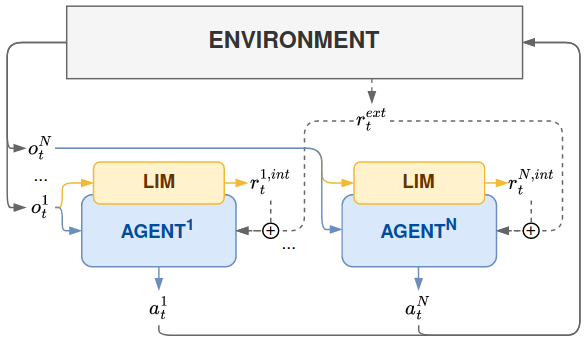
\includegraphics[width=0.71\textwidth]{Figures/JIM/archi_lim.png}
    \caption{Architecture for local intrinsic motivation (LIM), used as a baseline. Each agent has its own module for computing an intrinsic reward based on its local observation.}
    \label{fig:JIM:archi_lim}
\end{figure}

%As previously said, JIM can be used to augment any MADRL approach that fits in the CTDE paradigm. 
In the next section, we use JIM with QMIX~\citep{Rashid2018_QMIX}. We use the default QMIX architecture and hyperparameters, along with prioritised experience replay~\citep{Schaul2016_PER}. In all experiments, we compare three algorithms: 
\begin{itemize}
    \item \textbf{QMIX+JIM}, augmenting QMIX with joint exploration, as shown in Figure~\ref{fig:JIM:archi} and described in Section~\ref{sec:JIM:IntrRew}.
    \item \textbf{QMIX+LIM}, a degraded version of QMIX+JIM where local intrinsic motivation is used. Each agent generates its own intrinsic reward based solely on its local observation, using the same reward definition as JIM (see Section~\ref{sec:JIM:IntrRew}). The architecture for LIM (Local Intrinsic Motivation) is described in Figure~\ref{fig:JIM:archi_lim}.
    \item The original state-of-the-art \textbf{QMIX} algorithm~\citep{Rashid2018_QMIX} with no intrinsic motivation, used as a baseline. 
\end{itemize}
Note that the only difference between these three algorithms is the definition of the reward function given to each agent during training. The actual training and execution algorithms are identical. 

To ensure a fair comparison between JIM and LIM, we use different values for some specific hyperparameters in the two versions in order for them to have a similar number of trainable parameters. All hyperparameters used in our experiments are listed in Appendix~\ref{app:JIM:hpp}. The code used to run all experiments is freely available online\footnote{\url{https://github.com/MToquebiau/Joint-Intrinsic-Motivation}}.







% -------------------------------------------------------------------------------------------------

\section{Experiments}

In this section, we present a set of experiments to evaluate the exploration criterion of JIM when used along the state-of-the-art QMIX algorithm \citep{Rashid2018_QMIX}. First, we show the results in a synthetic discrete environment where the problem of relative overgeneralisation can be artificially tuned and observe that JIM helps alleviate this issue. Then, we test our approach on pseudo-realistic robotic tasks in a continuous environment and show that exploring the joint-observation space helps solve cooperative tasks with strong coordination requirements. Next, we present an ablation study by comparing JIM with two simpler versions that each lack one of the two exploration criteria described in Section~\ref{sec:JIM:IntrRew}, showing the advantage of combining the two. We show that JIM remains efficient with more than two agents. And, finally, we show that the centralised intrinsic motivation is more computationally efficient than the local version. 

\subsection{Addressing Relative Overgeneralisation}
\label{sec:JIM:Exp_Climbing}

\subsubsection{Environment Definition}

\begin{figure}
    \centering
    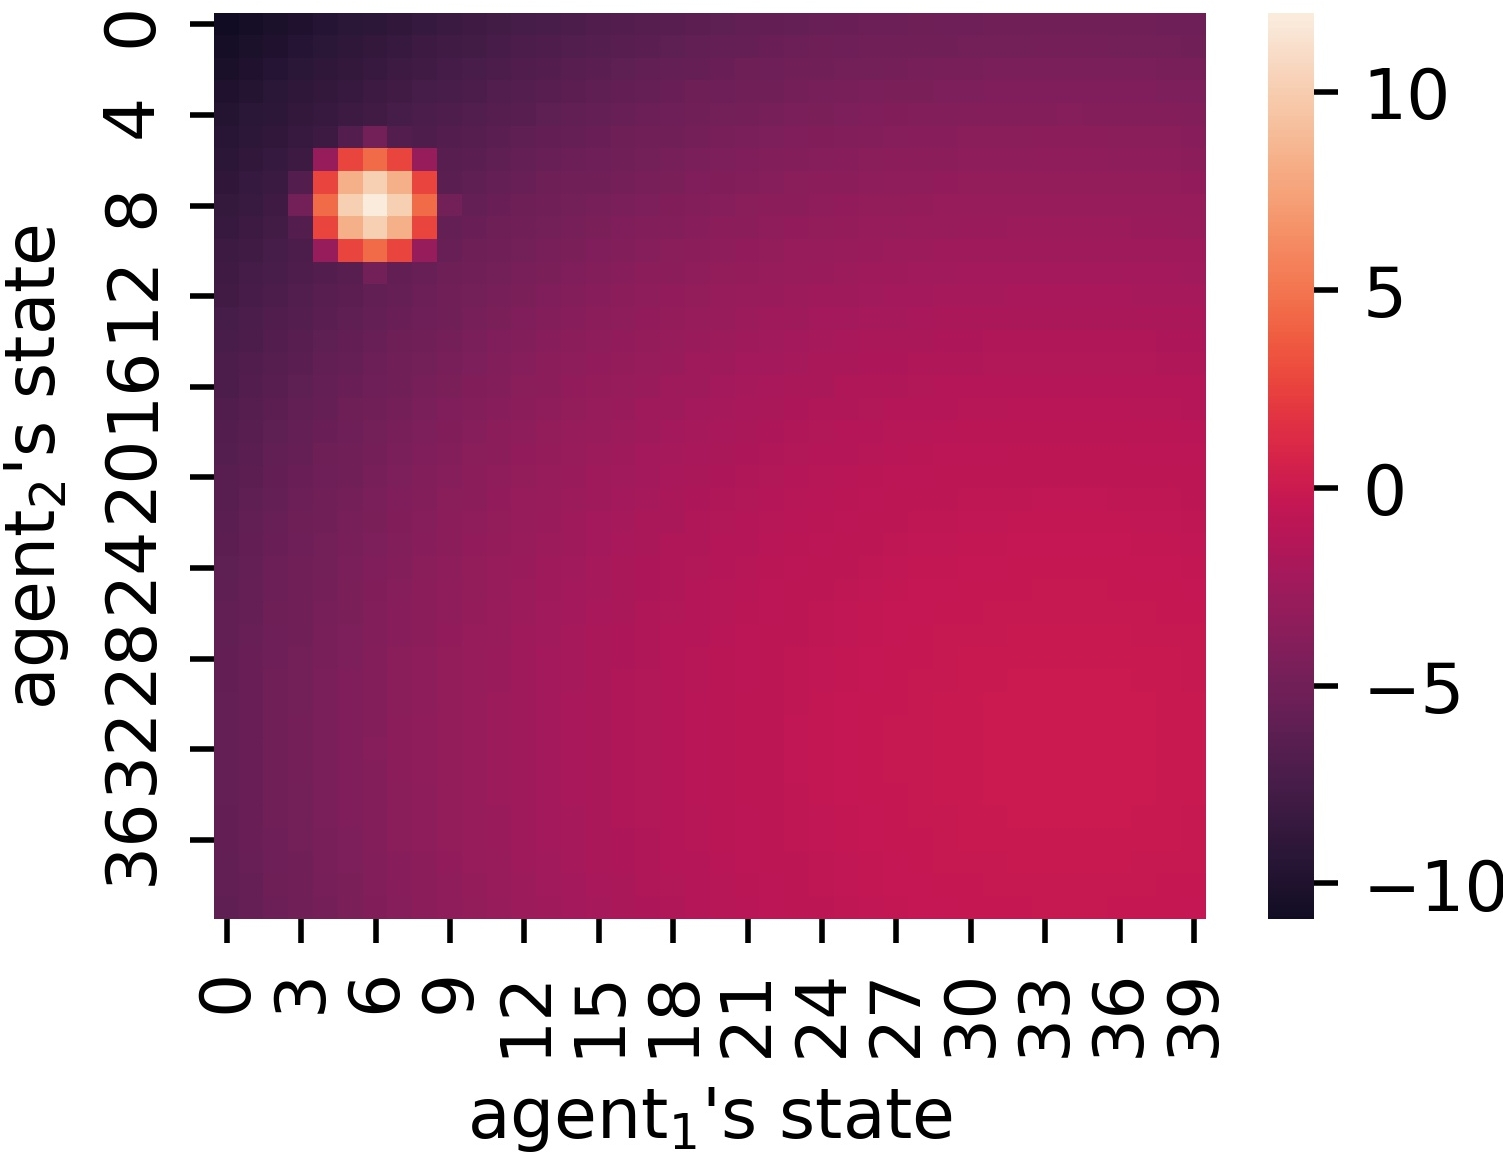
\includegraphics[width=0.5\linewidth]{Figures/JIM/ro_map30.jpg}
    \caption{Heat map of the rewards given for each state in the two-dimensional climbing game. Each axis show the positions of one agent. The combined position of the two agents yields a reward that is defined by Equation~\ref{eq:JIM:Climbing}. We distinguish clearly the high reward spike in the top-left of the environment and the low reward plateau in the bottom-right. The optimal strategy is to navigate towards the joint position corresponding to the high reward spike.}
    \label{fig:JIM:ro_map}
\end{figure}

To demonstrate how joint exploration helps solve the problem of relative overgeneralisation, we design a simple test environment that expands the example shown in Figure \ref{fig:JIM:ro_matrix}. This environment is a two-dimensional climbing game, inspired by previous works~\citep{Wei2018_MultiSoftQ}. In this environment, two agents can move on a discrete one-dimensional axis with $D$ possible positions. The two agents are denoted by their position, namely $\mathrm{x}$ (for the first agent) and $\mathrm{y}$ (for the second agent). At each time step, agents observe their position as a one-hot vector (e.g., for agent x, $o^\mathrm{x}_t=\{o^{\mathrm{x},i}_t=1\ \text{if}\ \mathrm{x}=i,\ 0\ \text{otherwise}\}_{0\leq i<D}$) and can choose between three actions: move in one direction or the other, or stay in position. They receive a reward corresponding to their combined position:
\begin{align}\label{eq:JIM:Climbing}
    \begin{split}
        r^{\text{ext}}_t(x,y;\delta)=\mathrm{max}\Bigl(&R^+-\frac{\delta}{D}\bigl[(x-r^+_x)^2+(y-r^+_y)^2\bigr],\\
        &R^--\frac{1}{8D}\bigl[(x-r^-_x)^2+(y-r^-_y)^2\bigr]\Bigr).
    \end{split}
\end{align}
The result of this formula is displayed in Figure \ref{fig:JIM:ro_map}. The reward combines two hyperboles in opposite corners: one narrow that culminates at $R^+$ at position $(r^+_x,r^+_y)$, and another much wider that plateaus at $R^-$ at position $(r^-_x,r^-_y)$. We set the optimal reward $R^+=12$ and the suboptimal $R^-=0$. The width of the optimal reward spike is controlled by the parameter $\delta$: a higher $\delta$ value yields a narrower spike. 

At the beginning of each episode, the agents are placed randomly on their respective axes. Each episode lasts $D$ steps, ensuring that all starting positions can reach all other positions on the axis. The goal of the agents is to find where to go to maximise the global return. The wide suboptimal hyperbole is deceptive as it is an obvious path for agents to minimise their loss. The optimal reward spike is difficult to find because it covers a small portion of the state space and is surrounded by very low rewards, but it guarantees much greater returns. We can vary the difficulty of the task by changing the width of this optimal reward spike: the narrower the spike, the harder it is to find. 

In this environment, we expect MADRL methods to struggle to find the optimal reward spike. Exploring local states could help but would not be sufficient to consistently solve the task. As the dimension $D$ of the local-state space is fairly small, local novelty rewards will quickly vanish and will not help agents find the optimal reward spike. Exploring the joint-observation space adequately is required in order to consistently find optimal rewards. As JIM will reward exploration until all combined positions $(x,y)$ are visited several times, agents will visit the optimal reward spike more often, thus helping them to learn the optimal coordinated strategy. 

\subsubsection{Results}

\begin{figure}
     \centering
     \begin{subfigure}[c]{\textwidth}
        \centering
        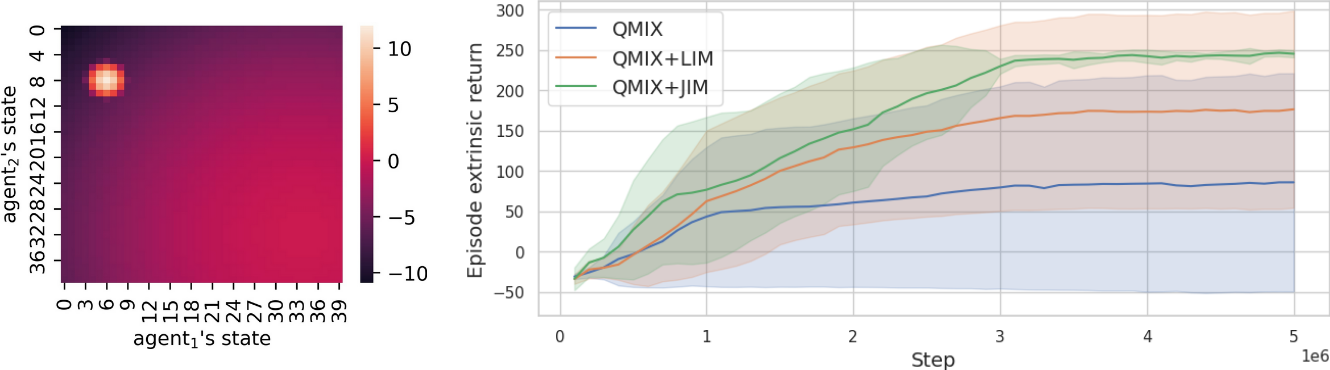
\includegraphics[width=\textwidth]{Figures/JIM/roR30.png}
        \caption{$\delta=30$}
        \label{fig:JIM:ro30}
     \end{subfigure}
     \vspace{1em}
     \begin{subfigure}[c]{\textwidth}
        \centering
        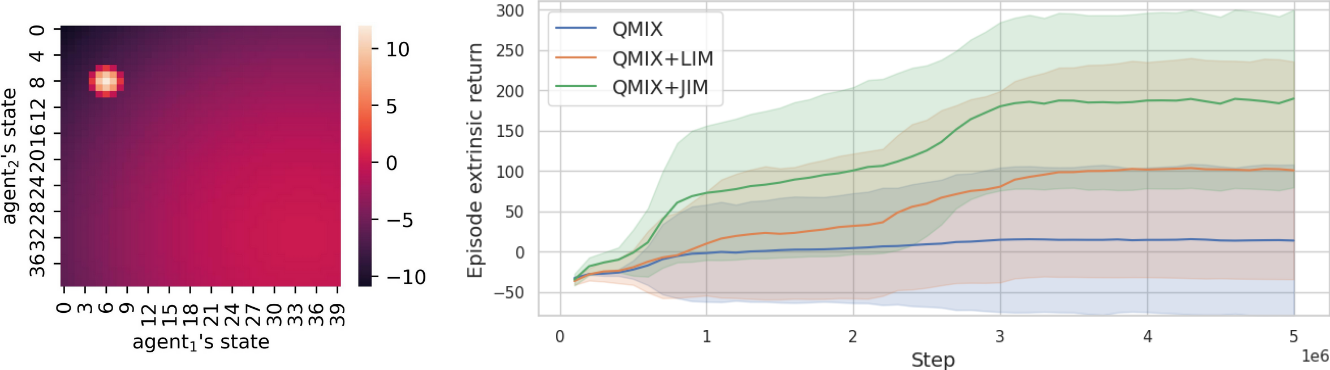
\includegraphics[width=\textwidth]{Figures/JIM/roR40.png}
        \caption{$\delta=40$}
        \label{fig:JIM:ro40}
     \end{subfigure}
     \vspace{1em}
     \begin{subfigure}[c]{\textwidth}
        \centering
        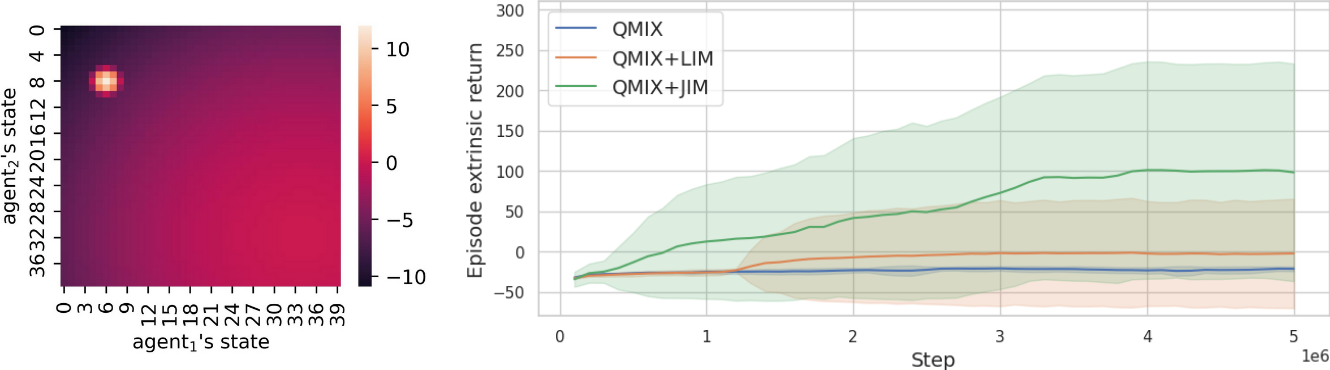
\includegraphics[width=\textwidth]{Figures/JIM/roR50.png}
        \caption{$\delta=50$}
        \label{fig:JIM:ro50}
     \end{subfigure}
     \caption{Performance of variants of QMIX in the climbing game, with three levels of difficulty. Each row corresponds to a different difficulty level, where difficulty is controlled by the width coefficient of the optimal reward spike $\delta$ (as defined in Eq. \eqref{eq:JIM:Climbing}). On the left are the heat maps representing the reward function in each instance. Increasing $\delta$ leads to a smaller optimal reward spike, thus making the task more difficult. On the right is shown the performance during training of QMIX with no intrinsic reward (QMIX), local intrinsic motivation (QMIX+LIM), and joint intrinsic motivation (QMIX+JIM) (mean and standard deviation shown for 15 runs each). We see that a slight decrease in the size of the optimal reward spike results in a considerable increase in the difficulty of the task.}
     \label{fig:JIM:ro_results}
\end{figure}

The results shown in Figure \ref{fig:JIM:ro_results} confirm the hypotheses formulated in the previous section. We show the performance of QMIX, QMIX+LIM, and QMIX+JIM across 15 independent runs each. Further, we present results in three difficulty levels dictated by the width of the optimal reward spike. The results clearly demonstrate the importance of exploring the joint-state space. QMIX alone manages to get a positive reward on the easy scenario, but its performance is lower and with a larger standard deviation compared to the two other algorithms, showing that some runs did not manage to find the optimal strategy. In the harder scenarios, QMIX's performance degrades strongly, never finding any positive reward in the hardest case. JIM clearly improves the performance of QMIX. In the easy scenario, QMIX+JIM consistently goes for the optimal reward spike. In the harder settings, it still performs well on average, even in the "very hard" scenario where the optimal reward spike covers only 0.013\% of all combined positions. The results of QMIX+LIM show that exploring the local-observation space helps agents find the optimal reward spike more often. However, it performs worse than JIM as it does not ensure that all combined positions are sufficiently explored. This shows that exploring the joint-observation space is crucial to allow agents to discover optimal coordinated behaviours.





\subsection{Coordination Task in a Continuous Environment}

\begin{figure}[h]
    \centering
    \setlength{\fboxsep}{0pt}
    \setlength{\fboxrule}{1pt}
    \fbox{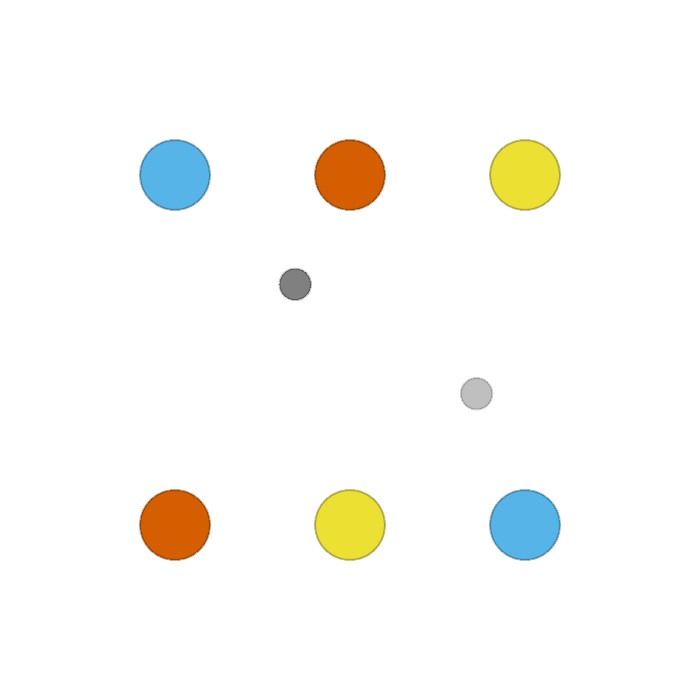
\includegraphics[width=0.4\textwidth]{Figures/JIM/push_buttons.jpg}}
    \caption{Coordinated placement task, agents are the small grey circles, the coloured circles represent landmarks the agents have to navigate on to gain rewards.}
    \label{fig:JIM:coord_place}
\end{figure}

\subsubsection{Environment Definition}

Next, we study how JIM scales to more realistic continuous environments and more complex tasks. We use the multi-agent particle environment (MPE;~\cite{Lowe2017_MADDPG}) to simulate a cooperative robotic task that requires a high degree of coordination. The state space of MPE is continuous: agents receive as observation a vector with their position in the two-dimensional space and relative positions and velocities of other entities. Agents navigate in a closed two-by-two-meter area by choosing between five discrete actions: move in any four cardinal directions or stay in place. The observation range is limited: agents only have information about entities that are in a range of 60 centimetres around them. 

We design a coordination task, named "\textit{coordinated placement}", where agents must position themselves over landmarks in order to maximise their returns. As shown in Figure \ref{fig:JIM:coord_place}, there are two sets of three coloured landmarks. The reward given at each time step depends on the placement of agents on the landmarks. The optimal state is having both agents placed on the orange landmarks, yielding a reward of +10 at each time step. The blue and yellow landmarks act as deceiving rewards, yielding much smaller rewards (+2 for blue, +1 for yellow). To increase the deceiving aspect of the blue and yellow landmarks, we also reward agents collectively by +0.5 if only one of them stands on one of these two colours. This leads to a relative overgeneralisation situation, as they will locally find that going on blue or yellow landmarks systematically leads to a reward, while this is not the case for orange. Only if agents explore their environment in a coordinated fashion, will they discover that they need to be both on orange to get the optimal reward signal. Importantly, this scenario features partial observability, with agents only having information about entities close to them. This means that agents do not necessarily see which landmark the other agent goes to. 

In this task, the observations of each agent consist in:
\begin{itemize}
    \item its personal information: its position and velocity $\mathtt{pos}_{\mathtt{self},x}$, $\mathtt{pos}_{\mathtt{self},y}$, $\mathtt{vel}_{\mathtt{self},x}$, $\mathtt{vel}_{\mathtt{self},y}$,
    \item information about the other agent: a boolean indicating if the other agent is visible or not, the relative position, and the velocity of this agent $\mathtt{is\_visible}_{\mathtt{agent}}$, $\mathtt{dist}_{\mathtt{agent},x}$, $\mathtt{dist}_{\mathtt{agent},y}$, $\mathtt{vel}_{\mathtt{agent},x}$, $\mathtt{vel}_{\mathtt{agent},y}$,
    \item for each landmark in the environment: a boolean indicating if the landmark is visible or not, the relative position of this landmark, and its colour as a one-hot encoding: $\mathtt{is\_visible}_{\mathtt{landmark}}$, $\mathtt{dist}_{\mathtt{landmark},x}$, $\mathtt{dist}_{\mathtt{landmark},y}$, $\mathtt{is\_red}$, $\mathtt{is\_blue}$, $\mathtt{is\_yellow}$.
\end{itemize}
Thus, the observation is a vector of dimension 43 containing this information. Relative positions of other entities (agent or landmarks) are actually the distance to the agent, normalised by their range of observation, i.e., 
$$\mathtt{dist}_{\mathtt{agent},x}=\frac{\mathtt{pos}_{\mathtt{agent},x}-\mathtt{pos}_{\mathtt{self},x}}{\mathtt{obs\_range}}.$$


\subsubsection{Results}

Experiments in the coordinated placement task demonstrate well the importance of exploring in a coordinated fashion. Figure~\ref{fig:JIM:coordplace_results} shows the performance across training of QMIX, QMIX+LIM, and QMIX+JIM, with 11 independent runs each. On the right is displayed the performance of each independent run at the last iteration of training. This helps to visualise the multiple modes in potential returns in this scenario. The coloured dashed lines give an insight into the level of strategy learnt by each run. These levels of strategy can be visualised with example trajectories displayed in Figure \ref{fig:JIM:coordplace_traj}. 

QMIX alone almost always goes for the blue landmarks, while sometimes settling for the yellow ones. This indicates that without actively exploring the environment, QMIX gets stuck because of deceptive rewards and is unable to find the optimal strategy. While QMIX+LIM seems slightly better than QMIX on the training curves, the individual run performance shows that LIM arguably performs worse. Two runs manage to find the optimal strategy, but LIM often performs poorly with only one agent on a blue or yellow landmark. This demonstrates that exploring the space of local observations can be helpful, as it pushes agents to explore the environment. However, it can also be misleading as they do not contain all the information about the current state of the environment. With JIM, exploring the joint-observation space clearly improves the quality of the chosen strategies. More than half of the time, QMIX+JIM finds the optimal reward signal and learns an effective strategy to go on orange landmarks, showing that JIM allows for more efficient exploration of coordinated behaviours. When agents do not find the optimal strategy, they stick with the best sub-optimal strategy to go both on blue. This shows that agents benefit from exploring the space of joint observations as they are directly linked to the obtained reward, whereas local observations lack crucial information to understand the global reward. 

The high standard deviation in the graph of Figure~\ref{fig:JIM:coordplace_results} is justified by the extreme gap in returns produced by the different levels of strategy. Note that this task is extremely sparse:
\begin{itemize}
    \item from a local perspective, because no guidance is given to agents to navigate towards any landmark;
    \item and from a joint perspective, as the optimal joint strategy is extremely marginal.
\end{itemize}
The deceptive rewards given by standing on blue or yellow make the suboptimal strategies very attractive. Without an explicit exploration strategy, QMIX is always attracted to the local optimum, similar to results found in the climbing game. Proper multi-agent exploration allows JIM to significantly improve the chances for QMIX to find the optimal strategy. 

\begin{figure}[t]
    \centering
    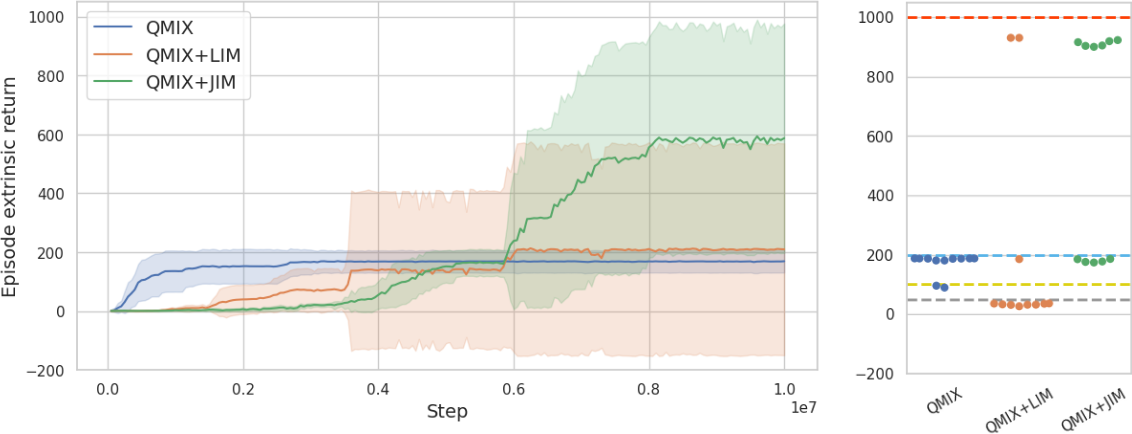
\includegraphics[width=0.95\textwidth]{Figures/JIM/coord_placeR.png}
    \caption{Performance of the three variants of QMIX in the coordinated placement task. The left shows the training curves with the mean and standard deviation across 11 independent runs each. The right graph displays the performance of each independent run at the last iteration of training. Dashed lines indicate the level of return obtained with different strategies: orange, blue, and yellow lines represent the return obtained if both agents are on landmarks of the related colour during 100 steps (the duration of an episode), and the grey line is for when only one agent is either on blue or yellow.}
    \label{fig:JIM:coordplace_results}
\end{figure}

\begin{figure}[t]
    \centering
    \centering
    \subcaptionbox{}{\includegraphics[width=0.22\textwidth]{Figures/JIM/traj1.png}}
    \subcaptionbox{}{\includegraphics[width=0.22\textwidth]{Figures/JIM/traj2.png}}
    \subcaptionbox{}{\includegraphics[width=0.22\textwidth]{Figures/JIM/traj3.png}}
    \subcaptionbox{}{\includegraphics[width=0.22\textwidth]{Figures/JIM/traj4.png}}
    \caption{Examples of trajectories in the coordinated placement task. Each image displays a different level of strategy, with (a) > (b) > (c) > (d): (a) optimal strategy with both agents on orange, (b) both on blue, (c) both on yellow, and (d) one on blue/yellow.}
    \label{fig:JIM:coordplace_traj}
\end{figure}





\subsection{Further Analysis}

\subsubsection{Ablation Study}

Next, we propose an ablation study to compare JIM with two derived versions of the reward: one with only the \textit{episodic exploration criterion} $N_{EEC}$ (JIM-EEC) and one with only the \textit{life-long exploration criterion} $N_{LLEC}$ (JIM-LLEC). Note that JIM-LLEC is actually equivalent to NovelD \citep{Zhang2021_NovelD} in this environment as the episodic restriction of NovelD (see Section \ref{sec:JIM:IntrRew}) would be ineffective in a continuous environment such as MPE. 

\paragraph{Results} Figure \ref{fig:JIM:ablation_results} shows the results of training these versions in the coordinated placement task, with 11 independent runs each. Both ablated algorithms perform significantly worse than JIM. First, the episodic bonus of JIM-EEC alone lacks the motivation for discovering unseen configurations. Thus, it explores less and is not able to find the optimal solution to the task. Meanwhile, without the episodic restriction, JIM-LLEC is less driven to have diverse trajectories, hindering its exploration abilities. This confirms that, as shown in a recent study \citep{Andres2022_EvalIntrRew}, the episodic restriction implemented in NovelD and other intrinsic rewards \citep{Raileanu2020_RIDE,Badia2020_NGU} is crucial for developing efficient exploration strategies.  Overall, this proves the importance of combining the two stages of exploration defined in $N_{LLEC}$ and $N_{EEC}$. 

\begin{figure}[t]
    \centering
    \includegraphics[width=0.95\textwidth]{Figures/JIM/ablationR.png}
    \caption{Ablation study of JIM in the coordinated placement task. The left graph shows the training curves with the mean and standard deviation across 11 independent runs each. The right graph displays the performance of each independent run at the last iteration of training. The two ablated versions only feature one of the two exploration criteria defined in Section \ref{sec:JIM:Algo}: JIM-EEC for $N_{EEC}$ and JIM-LLEC for $N_{LLEC}$. The results show the importance of combining the two criteria.}
    \label{fig:JIM:ablation_results}
\end{figure}




\subsubsection{Scaling Up to More Agents}\label{sec:JIM:Exp:scaling}

We evaluate JIM in a scenario with four agents using a modified version of the two-dimensional climbing game introduced in Section~\ref{sec:JIM:Exp_Climbing}. We modify the reward definition given Equation~\ref{eq:JIM:Climbing} to allow $N$ dimensions: 
$$
r^{\text{ext}}_t(\mathbf{p};\delta)=\mathrm{max}\left(R^+-\frac{\delta}{D}\sum_{i=0}^{N}(p_i-r^+_i)^2,R^--\frac{1}{8D}\sum_{i=0}^{N}(p_i-r^-_i)^2\right),
$$
with $\mathbf{p}=\{p_i\}_{0<i\leq N}$ the positions of the agents, $\delta$ the coefficient controlling the size of the optimal reward spike, $D$ the dimension of each agent's state, $R^+$ the maximum value of the optimal reward spike placed at position $\mathbf{r}^+=\{r^+_i\}_{0<i\leq N}$, and $R^-$ the maximum value of the suboptimal plateau placed at position $\mathbf{r}^-=\{r^-_i\}_{0<i\leq N}$. This formula yields the same results as the two-dimensional example shown in Figure~\ref{fig:JIM:ro_map} but in a $N$-dimensional space.

We use this extended version to experiment with a four-agent climbing game. As in the two-agent version, the reward function has a high reward spike in one corner of the space and a low reward plateau in the other corner, making relative overgeneralisation prone to arise. With more agents, the number of dimensions of the joint observation increases linearly (in this case: from 80 dimensions with two agents to 160 with four agents) while the number of possible states increases exponentially, making the search for the optimal strategy significantly more challenging.

To compensate for the increased size of the state space, we have to make the optimal reward spike larger for the task to be solvable by QMIX. In the four-agent experiments, we use $\delta=0.9$. 
Also, with four agents we had to lower the initial value of the $\epsilon$ parameter of QMIX for its $\epsilon$-greedy strategy. We found that increasing the number of agents led to bad results with the default $0.3$ initial value of $\epsilon$. With this hyperparameter set to $0.1$, the results were significantly better. This is likely due to the fact that agents choose separately if they explore or exploit, meaning that increasing the number of agents leads to more randomness in the selection of each joint action. 

\begin{figure}
    \centering
     \includegraphics[width=0.8\textwidth]{Figures/JIM/climb4R.png}
    \caption{Training performance of QMIX, QMIX+LIM and QMIX+JIM in the four-agent climbing game. The top graph shows the mean and standard deviation across 11 runs each, the bottom graphs display all single runs for QMIX (left) and QMIX+JIM (right).}
    \label{fig:JIM:climb4_results}
\end{figure}

\paragraph{Results} Figure~\ref{fig:JIM:climb4_results} shows the results in this scenario for 11 independent runs each. As with previous experiments, JIM improves the performance of QMIX by upgrading its exploration capabilities. Taking a closer look at the results reveals that QMIX and QMIX+LIM find the optimal solution in respectively $2$ and $0$ runs out of the $11$, while QMIX+JIM finds the optimal solution in $8$ out of $11$ runs in the allocated time (see Figure~\ref{fig:JIM:climb4_results}-bottom).  
The two positive results for QMIX can be attributed to beneficial initial conditions as QMIX never reaches the optimal performance otherwise. This is not the case with QMIX+JIM, which shows robustness to initial conditions thanks to active exploration of the environment. In fact, the impact of JIM becomes evident when looking at curves from individual runs, where we consistently observe significant performance enhancements subsequent to a minor initial drop in efficiency. This phenomenon reflects a deliberate shift towards exploring novel approaches when the system would otherwise remain stagnant. This is unique to JIM, as  QMIX+LIM never succeeds in finding the optimal solution, advocating for the benefits of using a global, rather than local, intrinsic reward for exploration. 





\subsubsection{Cooperative Task with no Coordination Need}

\begin{figure}[h]
    \centering
    \setlength{\fboxsep}{0pt}
    \setlength{\fboxrule}{1pt}
    \fbox{\includegraphics[width=0.4\textwidth]{Figures/JIM/coop_push.png}}
    \caption{Cooperative box pushing task, agents are the small grey circles, the green circle in the middle is an object to deliver to the landmark in the bottom right corner.}
    \label{fig:JIM:cooppush}
\end{figure}

To study coordinated exploration further, we experiment with a cooperative task that depends less on coordination. We design a cooperative box-pushing task that requires agents to push an object and place it on top of a landmark. Figure~\ref{fig:JIM:cooppush} shows a screenshot of this scenario. At the start of each episode, the landmark is randomly placed in any one of the four corners. The initial positions of the agents and the object are randomly set. If the agents manage to push the object and place it on the landmark, the episode ends early and they receive a reward of +100. Agents also get a small penalty of -1 at each time step to reward faster strategies. 

In this setting, observations are defined as:
\begin{itemize}
    \item its personal information: its position and velocity $\mathtt{pos}_{\mathtt{self},x}$, $\mathtt{pos}_{\mathtt{self},y}$, $\mathtt{vel}_{\mathtt{self},x}$, $\mathtt{vel}_{\mathtt{self},y}$,
    \item information about the other agent: a boolean indicating if the other agent is visible or not, the relative position, and the velocity of this agent $\mathtt{is\_visible}_{\mathtt{agent}}$, $\mathtt{dist}_{\mathtt{agent},x}$, $\mathtt{dist}_{\mathtt{agent},y}$, $\mathtt{vel}_{\mathtt{agent},x}$, $\mathtt{vel}_{\mathtt{agent},y}$,
    \item information about the object: a boolean indicating if the object is visible or not, the relative position, and the velocity of this object: $\mathtt{is\_visible}_{\mathtt{object}}$, $\mathtt{dist}_{\mathtt{object},x}$, $\mathtt{dist}_{\mathtt{object},y}$, $\mathtt{vel}_{\mathtt{object},x}$, $\mathtt{vel}_{\mathtt{object},y}$,
    \item and information about the landmark: a boolean indicating if the landmark is visible or not and the number of the corner it is located into (from 1 to 4): $\mathtt{is\_visible}_{\mathtt{landmark}}$, $\mathtt{corner}_{\mathtt{landmark}}$.
\end{itemize}
The observation is a vector of dimension 16 containing this information. Similarly to the coordinated placement task, this setting is also partially observable. 

\begin{figure}
    \centering
    \includegraphics[width=0.8\linewidth]{Figures/JIM/cooppushR.png}
    \caption{Training curves of the three variants of QMIX in the cooperative box pushing task, with the mean and standard deviation across 11 runs each.}
    \label{fig:JIM:push_results}
\end{figure}

\paragraph{Results} Figure \ref{fig:JIM:push_results} shows the results in the cooperative push scenario (median and confidence interval shown for 11 runs each). First, we observe that QMIX alone performs very poorly as it is unable to find the solution to the task. The high sparsity of the reward function makes it impossible for agents to discover the objective with random exploration of the environment. Second, we see that JIM and LIM achieve similar levels of performance. While coordination can help agents perform well, it is actually not a requirement for this task. In fact, one agent alone is able to push the object and place it on the landmark. Thus, exploring the space of joint configurations is not helpful in this scenario. This shows however that actively exploring the environment is crucial in tasks where the reward function is very sparse. 




\subsubsection{Time Consumption}

\begin{figure}
    \centering
    \includegraphics[width=0.8\textwidth]{Figures/JIM/time.png}
    \caption{Training curves of QMIX, QMIX+LIM, and QMIX+JIM in the coordinated placement task with execution time on the x-axis. In our implementation, using JIM increases training time by 31\%, and with LIM by 62\%.}
    \label{fig:JIM:time}
\end{figure}

Finally, we show another advantage of having a single, centralised intrinsic motivation. While LIM and similar approaches in previous works \citep{Iqbal2019_MultiExplore,Du2019_LIIR,Wang2020_EITI} require computing one intrinsic reward for each agent, JIM only computes one intrinsic reward for the whole group of agents. This makes JIM significantly more efficient to run, with LIM being approximately 24\% slower than JIM to train, as shown in Figure~\ref{fig:JIM:time}. 










% -------------------------------------------------------------------------------------------------

\section{Conclusion}

In this chapter, we present an algorithm for joint intrinsic motivation (JIM), which is the first method to reward active exploration of the joint-observation space. It can be integrated to enhance any MADRL algorithm that uses centralised training with decentralised execution. By combining JIM with the state-of-the-art QMIX algorithm, we demonstrate that it outperforms the original QMIX implementation, as well as a modified QMIX algorithm using local curiosity. We show that active exploration is a key component for multi-agent learning in environments with sparse rewards. Moreover, joint exploration enables the discovery of optimal coordinated behaviours that would be hard to find otherwise as they necessitate a high level of coordination between agents. 

This shows the importance of using joint observations in the process of computing intrinsic rewards for a multi-agent system. In fact, the joint observation is the best estimate of the global state of the environment available for the agents. Using it allows more efficient learning of multi-agent joint behaviours and is computationally less expensive than having to compute local intrinsic rewards for each agent. These results should encourage research on how joint observations can be used in other kinds of intrinsic rewards to shape the agents' behaviour further. 



\Chapter{Language-augmented multi-agent learning}{Learning to communicate with a pre-defined, discrete language}

\label{ChapterComm} 

\section{Introduction}

% FIGURE communication with emergent language vs pre-defined: "we want to show how we can teach language to agents, and what benefits it gives. while there is a cost to pay for teaching langugage to agents, the benefits are great"

% Context
Multi-agent deep reinforcement learning (MADRL) aims at learning how to behave in social settings where multiple intelligent agents interact. This social component adds complexity to the learning process, requiring agents to master additional skills to engage in these environments properly. 
One essential skill in such settings is communication, playing a crucial role in facilitating social interactions. It is observed in various forms across many social animal species~\citep{Smith2003_AnimalSignals, Searcy2010_AnimalCommEvo}, and of course, humans, where it enables a great range of social abilities from sharing information about local observations to negotiation, knowledge transmission, and teaching~\citep{Greene2003_Communication}. 
Taking inspiration from these natural systems, groups of artificial agents can certainly benefit from being able to communicate with partners for sharing information gathered locally and expressing their intentions. 

% Differentiable emergent communication
As described in Section~\ref{sec:MADRL:EmergentCommunication}, learning to communicate accounts to learning (i) \textit{what information to transmit} and (ii) \textit{how to transmit it}. A solution provided by MADRL is \textbf{differentiable emergent communication}, where agents develop communication protocols from scratch driven mainly by the goal of maximising returns. Using differentiable neural networks to produce messages allows learning communication as a sub-module of the policy through gradient back-propagation of the RL objective~\citep{Zhu2024_MACSurvey}. In other words, the problem of learning (i) and (ii) is entirely entrusted to the deep RL algorithm. Whether this approach could lead to the emergence of a language is itself debatable~\citep{Lazaridou2020_DeepEmergentComm, Galke2022_Emergent}. Some approaches try to improve emergent communication in this regard, as we will see in Section~\ref{sec:LAMAC:RW_LanguageDef}. However, in MADRL research, this problem is usually disregarded to focus on how communication improves performance. 

% Problem with DEC
However, this approach suffers from significant drawbacks. One important issue is the \textbf{lack of interpretability} of the emerging communication systems. Since multi-agent systems are targeted toward applications in human-populated environments, interpretability becomes an important matter~\citep{Mikolov2018_RoadmapMachineIntell}. If provided, it would enable transparent human-agent interactions and offer tools for evaluating the reasoning of learnt artificial agents. Researchers have proposed techniques to analyse the resulting communication processes by clustering messages based on state-message correlation~\citep{Lin2021_GroundMAC, Tucker2021_DiscreteEC, Li2022_EmDicrComm, Karten2023_InterpretEmComm}, identifying patterns in emergent languages~\citep{Havrylov2017_EmergenceLang}, or mapping emergent languages to known entities~\citep{Kottur2017_NaturLangEmerg}. These approaches require tedious analysis of the emergent languages, offer no guarantees of success, and need to be applied separately to each independently trained group of agents, as each one develops its own unique communication protocol. 
Another approach is to bias the emerging communication protocols to carry meaning related to external modalities (e.g., visual inputs, actions, real-world concepts). These grounding approaches, reviewed in Section~\ref{sec:LAMAC:RW_Grouding}, guide emergent communication by informing potential useful meanings to convey in the communicated messages. However, this does not solve the interpretability issue, as emergent languages still require some post hoc analysis to be, still imperfectly, interpreted~\citep{Lin2021_GroundMAC, Tucker2021_DiscreteEC}. 

% Advantages of natural languages
A suitable solution to the interpretation issue would be to \textbf{have agents converse using a language} understood by humans. 
Rather than trusting the agents to develop a functioning communication system on their own, teaching them a pre-defined (as opposed to "emergent") language would have many benefits. 
Natural languages have evolved into very efficient communication systems, enabling the vast range of social interactions we take part in. Language allows describing parts of our environments to share local information with others. It allows expressing needs to explain intentions, negotiate, or ask for help. As a shared tool for expressing meanings, it supports the development of culture and the transmission of knowledge. 
In addition, language has been shown to play an important role in the intellectual development of children~\citep{Vygotsky1934, Tomasello2009_Cultural}. This idea has motivated research on language-augmented learning, reviewed in Section~\ref{sec:LAMAC:RW_LARL}, to study how language can be used to guide the learning of artificial agents. 
Overall, providing a language to agents is a way to guide training by introducing a bias on how the environment should be understood and how communication should be conducted. If done successfully, the resulting language-augmented agents would be easier to evaluate, interact and bond with~\citep{Crandall2018_CoopWithMachines, Mikolov2018_RoadmapMachineIntell, Liu2022_ChildChatbotReading}. 

% Chapter objective
While some previous works have experimented with language-based communication, to the best of our knowledge, no study applied it to embodied multi-agent environments. Indeed, learning to communicate with a pre-defined language to solve an embodied task presents its own challenges. It requires a reliable source of language examples and an algorithm capable of learning a language without interfering with policy learning. In this chapter, we propose a solution to these issues by training MADRL agents to produce language utterances that describe their observations. 
The learning algorithm, detailed in Section~\ref{sec:LAMAC:Method}, trains agents to solve the multi-agent task while grounding their observations in language examples. This serves a double purpose: (i) \textbf{enabling agents to learn language-based communication}, while (ii) \textbf{guiding representation learning} by providing an efficient way of extracting valuable information from the world. To allow this, we provide agents with language examples that show how the pre-defined language should be used to describe observations. This data is used to train supervised language objectives concurrently to training on the multi-agent RL objective.  

Through a series of experiments, we show that the cost we pay to train language-augmented agents is easily justified by the advantages brought by language. We demonstrate that language-based communication is easier to learn and more efficient than emergent communication baselines, as the pre-defined language is made to compress the informational content of observations to fit the needs of the task at hand. Having agents communicate with language also enables interesting capacities, namely:
\begin{itemize}
    \item \textbf{better generalisation} of experience to changes in the environment,
    \item \textbf{better adaptation} to new partners,
    \item and easy \textbf{interactions} between humans and the learnt agents.
\end{itemize}
Crucially, language guidance helps agents structure their understanding of the world with linguistic concepts, resulting in faster learning. 


% TABLE advantages of communicating with language
% \begin{table}[]
%     \begin{tabular}{cccc}
%     \hline
%                     & Emergent-Continuous & Emergent-Discrete & Language \\ \hline
%     Training scheme & \begin{tabular}[c]{@{}c@{}}RL from task reward \\ (+ Grounding)\end{tabular} & \begin{tabular}[c]{@{}c@{}}RL from task reward \\ (+ Grounding)\end{tabular} & Supervised \\
%     Bandwidth & High & Low & Low \\
%     \begin{tabular}[c]{@{}c@{}}Interpretability\\ \& Interaction\end{tabular} & Very difficult & Difficult & Straightforward \\ \hline
%     \end{tabular}
%     \caption{Comparison of different communication learning paradigms: emergent communication with either continuous (Emergent-Continuous) or discrete (Emergent-Discrete) signals, and language-based communication (Language). The training approach for emergent communication is mainly based on RL, with the possibility of adding some grounding, while language is learnt with supervision. The bandwidth of continuous signals is very high, while the discrete symbols of Emergent-Discrete and Language allow more compression. Finally, Language allows straightforward interpretation of communication acts and interaction with agents, while both interpretability and interaction are difficult with emergent discrete language, and even more complex with continuous signals that can take an infinite number of different values.}
%     \label{tab:LAMAC:CommStrats}
% \end{table}





% -------------------------------------------------------------------------------------------------

\section{Language and Communication in Artificial Intelligence: Related Works}\label{sec:LAMAC_RW} 

\subsection{Language and Emergent Communication}\label{sec:LAMAC:RW_LanguageDef}

% What's a language
A language can be defined as a shared set of conventions for expressing meaning~\citep{Pinker1990_NaturalLang, Steels1995_SelfOrgVoc}. In natural languages -- i.e., languages that emerged naturally in human cultures --, large vocabularies and complex grammar systems form a rich sets of shared conventions allowing humans to communicate about a large variety of different matters. This is permitted by two key properties of these languages. First, natural languages are combinatorial. They use basic building blocks (e.g., phonemes, syllables) and combine them to construct rich semantic constructs that can hold complex meanings~\citep{Zuidema2018_Combinatorial}. Second, they are compositional: the meaning of a combination of language blocks is a function of the meaning of the combined blocks~\citep{Smith2003_CompoEmerg}. These properties allow natural languages to express a seemingly infinite number of different meanings from a finite set of different symbols. Importantly, they allow to compress information to ensure less costly communication acts and simpler language transmission~\citep{Sigurd2004_ZipfRevisit, Gibson2019_EfficiencyShapeLang}. As a result, natural languages have been shown to have a nearly optimal expressiveness to compression ratio~\citep{Kirby2015_CompressionComm, Gibson2019_EfficiencyShapeLang}, ensuring high efficiency of communication acts and making these languages easier to learn~\citep{Carr2016_CulturalEvoLang}. 

    Experiments involving emergent communication were initially aimed at studying how such languages emerge and evolve in populations of independent agents~\citep{Steels1995_SelfOrgVoc, Nowak1999_LanguageEvo, Vogt2005_EmergenceCompo, Brighton2005_LanguageAsEvo, Kirby2015_CompressionComm}. These experiments showed that languages are cultural adaptive processes that evolve through their numerous independent uses~\citep{Steels1995_SelfOrgVoc, Kirby2015_CompressionComm, Christiansen2008_BrainShapeLang}, and are shaped by environmental~\citep{Perfors2014_WorldShapeLang} and physiological~\citep{Christiansen2008_BrainShapeLang} constraints. Iterated learning experiments studied the transmission of language between successive generations of language users~\citep{Smith2003_IteratedLearning, Vogt2005_EmergenceCompo, Kirby2015_CompressionComm}. They revealed that learning from a limited set of language acts results in a transmission bottleneck ultimately favouring combinatorial and compositional structures in languages. In this context, differential emergent communication has also been used to extend the study of language evolution to the multi-agent reinforcement learning setting~\citep{Havrylov2017_EmergenceLang, Kottur2017_NaturLangEmerg, Lazaridou2017_EmergNaturalLang, Chaabouni2019_AntiEfficient, Rita2022_PopHetero}. To this end, it has an interesting potential for studying the impact of embodied learning on the evolution of language~\citep{VanEecke2022_LangGameMARL}.

However, in the MADRL context, emergent communication, in its differentiable form, has been re-purposed as a tool for optimising multi-agent policies~\citep{Zhu2024_MACSurvey}. In this new task-oriented setting, the emergence of language properties is disregarded to focus on performance on a given multi-agent task. Differentiable communication fits well in the neural paradigm of deep RL, allowing end-to-end learning of communication mechanisms without supervision~\citep{Foerster2016_DIAL, Sukhbaatar2016_CommNet, Mordatch2018_GroundedCompo, Jiang2018_ATOC, Jaques2019_SocialInfluence, Singh2019_IC3Net, Das2019_TarMAC, Kim2018_SchedNet, Zhang2019_VBC, Han2023_MBC}. But, while emergent communication is almost always shown to be effective (i.e., improving performance), multiple works have highlighted its important limitations for this new purpose~\citep{Kottur2017_NaturLangEmerg, Lazaridou2020_DeepEmergentComm}. Emergent languages trained only from return maximisation lack the advantageous qualities of natural languages, namely compositionality~\citep{Galke2022_Emergent}, compression~\citep{Chaabouni2019_AntiEfficient}, and consistency of used signals~\citep{Kottur2017_NaturLangEmerg}. 
\citet{Bouchacourt2018_HowAgentsSee} also showed that agents trained with differentiable communication are able to successfully communicate about noisy inputs. This shows that they have not learnt to communicate about underlying concepts present in their input data, but rather land on an arbitrary consensus on how to represent their observations. 

These issues demonstrate that learning emergent communication only from communication success does not result in structured languages. However, by refining the training process, emergent languages can recover some qualities of natural languages. For example, compositionality can be improved by constraining the size of the vocabulary~\citep{Mordatch2018_GroundedCompo} or increasing the size of the population~\citep{Chaabouni2022_EmCommScale, Rita2022_PopHetero}. Consistency of used signals can also be improved by maximising the mutual information between the input data and the generated messages~\citep{Eccles2019_EmCommBiases}. 

These numerous works on emergent communication help us identify the important qualities of natural language and how they enable efficient communication. They show that emergent languages can be driven to emulate these qualities, provided the right experimental designs and algorithmic choices. Crucially, they show that communication performance does not necessarily imply communication efficiency and, thus, that learning emergent communication from return maximisation alone produces poor communication mechanisms.  




\subsection{Improving Emergent Communication with Grounding}\label{sec:LAMAC:RW_Grouding}

% Grounding definition
Previously cited issues of differentiable emergent communication may be all connected to a more fundamental problem: a lack of conceptual content in communicated signals. This can be related to the \textbf{symbol grounding problem}, defined by \citet{Harnad1990_SymbolGrounding} as the problem of associating meaning from the environment to a priori meaningless symbols. In natural languages, words and sentences carry meaning that is independent of the language itself: e.g., the symbol "apple" encodes a meaning that does not depend on the English language to exist. This consensus on how to express universally recognised meanings allows effective communication about these meanings. In the language evolution domain, the problem of grounding is crucial to understand how humans learn and use language~\citep{Siskind1992_LangAcquis, Brent2001_VocDev}, and how languages can emerge from grounded linguistic interactions~\citep{Steels2000_AIBO, Vogt2002_PhysicalGrounding, Steels2015_TalkingHeads, Nevens2020_ConceptLearn, Botoko2024_LingConvent}. 

% DEC lacking grounding
In Section~\ref{sec:MADRL:EmergentCommunication}, we defined differentiable emergent communication as learning a differentiable sub-step of the agent's policy to maximise the obtained returns. This training process does not have any requirement on how communication actually occurs: if it carries any information, if messages have any impact on the receivers, or if it has any kind of structure. While we can expect agents to learn to communicate about their observations, learning only from RL feedback gives no guarantee of this~\citep{Lowe2019_Pitfalls}. Indeed, we expect agents to learn to extract meaningful concepts from their input data, with only task performance as guidance. This is probably too much to expect. As shown by \citet{Bouchacourt2018_HowAgentsSee}, a more probable outcome is that agents will find an arbitrary consensus on how to communicate about observations, without actually using any concepts that appear meaningful to us. This may be one source of explanation for the issues cited in the previous section: \textit{how can symbols be combined and composed if they do not carry meaning?} This is also a fundamental problem for interpretation, as trying to understand potentially meaningless utterances would be pointless. 

% Grounding approaches
Therefore, instead of relying on return maximisation to produce meaningful communication, agents could benefit from explicitly grounding their messages into meaningful concepts. To do so, we can bias the training process by forcing communication to carry meaning related to external modalities. This can be achieved by adding auxiliary learning tasks on which agents are either pre-trained or trained on concurrently to RL training. By external modalities, we mean any source of meaning that is independent of the agents and the task at hand. The environment, and how the agents perceive it, is a source of meaning that can be leveraged to infuse meaning in the information transmitted between agents. By learning to reconstruct the input data from the communicated messages, agents can learn to maximise the informational content about their observations in their messages~\citep{Lowe2020_S2P, Lin2021_GroundMAC, Karten2023_CompoConcept, Karten2023_IMGSMAC}. Another external source of meaning is natural language. When used to describe the environment, it associates important environmental configurations with words and sentences. It also purposefully discards worthless or superfluous information in the input signals by simply not putting words on these. Learning to make these connections, by associating observations with corresponding language descriptions, allows agents to identify key concepts of their input space to communicate about~\citep{Lazaridou2017_EmergNaturalLang, Das2017_CoopVisDial, Havrylov2017_EmergenceLang, Lazaridou2020_MACNatLang, Tucker2021_DiscreteEC}. These grounding approaches are a way to help agents learn meaningful communication with the support of the additional supervised learning objectives. It helps fill the gap of task-oriented RL, by providing guidance for learning to identify concepts.


% In the neural paradigm of differentiable communication, agents starts with a randomly initialised neural network for generating messages. Training this communication policy network with RL drives its parameters to generate messages that improve the obtained returns. However, this training process does not have any requirement on how communication actually occurs: if it carries any information, if messages have any impact of the receivers, or if it has any kind of structure. Thus, this is not a surprise that learning differentiable communication only from a task-oriented RL feedback does not produce efficient languages. 

% This is even more unsurprising when looking back at our definition of differentiable communication: as a differentiable sub-step of the action-selection process. In other words, the message generation function is a sub-function of the policy. But, in this neural paradigm, the policy acts as a black box of which only the input and output are explicitly defined and easily interpretable. Thus, another way of looking at differentiable communication is to see it as probing into this black box: looking at the output of a particular module of the policy. Trying to interpret the meaning of this signal is a matter of explaining the inner reasoning of a neural network, which is a research problem in itself~\citep{Samek2021_ExplainDNN}. 
% While it can be expected that the probed message has some kind of connection to the final output (here the agent's action), understanding the nature of this connection and the informational content of the message is likely to be a difficult task. 



\subsection{Learning Natural Language}\label{sec:LAMAC:RW_NaturalLang}

Taking this to the extreme allows learning to use natural language for communication, by learning to replicate human-generated sentences and generating natural language messages~\citep{Wang2016_LangGameInteract, Das2017_CoopVisDial, Lewis2017_Deal, Agarwal2019_CommunityRegul, Lee2019_CounteringLDrift, Lazaridou2020_MACNatLang, Gupta2021_DynamicPop}. Using natural language instead of emergent communication does not completely solve the problem of learning to communicate. Agents still need to understand what symbol relates to what meaning and how compositional structures describe different environmental configurations. 
But, it solves the problem of interpretability, by making agents converse with the same tools as human experimenters. 

% Learning language requirements
However, learning to use a pre-existing language requires access to demonstrations of this particular language. Thus, to teach natural language to agents, previous works have been restricted to training environments that feature a large amount of language examples. Such environments are usually centred around language, with language being either the agents' observation or action domain. 
For example, the \textit{Lewis signalling games}~\citep{Lewis1969_Convention}, or \textit{language games}~\citep{Steels1995_SelfOrgVoc, Steels2000_AIBO}, usually involve interactions between two agents: one speaker and one listener; where the goal is for the speaker to transmit some information about its observation and for the listener to correctly interpret the incoming message. This framework can be used for describing natural language processing tasks, such as translation~\citep{Lee2018_EmergentTranslation, Lee2019_CounteringLDrift, Lu2020_CounterLangDrift} or image captioning~\citep{Lee2019_CounteringLDrift, Lazaridou2020_MACNatLang, Gupta2021_DynamicPop}, allowing to exploit large datasets of language examples. 
Another example is \textit{visual dialogue}~\citep{Das2017_CoopVisDial, Agarwal2019_CommunityRegul}, which can benefit from datasets of conversation about images to learn communication with natural language.

% Limits of language-centered envs
While these settings show successful instances of learnt language-based communication, they fail to emulate the complete role of language in human communication: as a tool for supporting multi-agent interactions. In language-centred environments, agents lack of embodiment: they are defined only by their language abilities and have no physical interactions independent of the language task. We argue that this limits both:
\begin{itemize}
    \item the complexity of the learning problem: in embodied, multi-agent settings, communication is not necessarily central to the task, agents need to learn when and how to use it best for the task at hand;
    \item the actual language abilities of these agents: physical interactions play an important role in learning language, thus, learning only from language data, even with visual grounding, can result in incomplete knowledge of the meaning behind natural language symbols. 
\end{itemize}
In Section~\ref{sec:LAMAC:Method}, we propose an approach for alleviating these issues, making a step towards learning language in multi-agent robotic settings. 

% LLMs 
Lastly, when it comes to using natural language almost as proficiently as human beings, \textit{large language models} (LLMs) are now widely recognised as the most evident choice. Thanks to their extremely large architectures, extensive pre-training on large amounts of human-generated text, and use of RL to better fit human preferences~\citep{Christiano2017_RLHF, Ouyang2022_InstructGPT}, they excel in generating human-like text. With some fine-tuning, they can easily be adapted to work with multi-modal inputs, allowing to handle visual and even behavioural modalities~\citep{Driess2023_PaLME}. With specific prompting techniques, LLMs can be driven to exhibit particular behaviours and even adopt personas~\citep{Li2023_CAMEL, Park2023_LLMtown, Perez2024_CulturalEvo}.
All these features allow to define \textit{agent-based LLMs}~\citep{Li2023_ToMLLM, Liu2024_HLA, Zhang2024_CoELA} for studying multi-agent settings with LLMs mimicking human reasoning. 
There is no doubt that these capabilities have an interesting potential for handling more complex multi-agent tasks and interacting with artificial agents. 
However, there are still some issues and limitations preventing the wide adoption of LLMs. Their extremely high pre-training and fine-tuning costs prevent their adaptation to specific settings. 
While using LLMs "out-of-the-box" as a human-like language module can enable general language capacities, this inevitably means that the language-learning phase is lost. One goal of this work is to demonstrate that the act of learning the language can guide the agents in learning how to behave in their environment. In the next section and later in the experiments (see Section~\ref{sec:LAMAC:Experiments}), we provide arguments and experimental results to back this claim. 







\subsection{Language-Augmented Learning}\label{sec:LAMAC:RW_LARL}

An important idea at the core of this work is the fact that language supports learning and intellectual development. In developmental psychology,~\citet{Vygotsky1934} has shown the central role of language and language-based social interactions in the intellectual development of children. Language serves structured reasoning as a way to describe the learning environment, set goals based on previously experienced or observed interactions, imagine new goals based on the composition of known, language-expressed goals, and internalise social interactions for supporting later goal-based learning~\citep{Vygotsky1934, Piaget1952, Tomasello2009_Cultural, Lupyan2012_WhatWordsDo}. 
 % the acquisition of knowledge

Following these observations, researchers have explored different ways by which language can guide the training of RL agents. Language can be used to ground the agents' understanding of their environment, by learning to describe observed situations~\citep{Ruis2020_gSCAN, Hanjie2021_EMMA, Hill2021_Grounded}. This allows efficient representation learning and better generalisation to unseen environmental configurations and even different domains with similar entities~\citep{Narasimhan2018_Transfer}.
Describing the world with language can also enable the prediction of future outcomes~\citep{Huang2022_InnerMonol, Lin2023_Dynalang, Nottingham2023_DECKARD}, allowing language-grounded model-based RL. 
Like with human beings, language can be used to express goals~\citep{Lynch2021_MCIL}. By expressing goals with language, agents can learn to associate the experienced trajectories with the linguistic concepts in the observed goals. In such goal-directed learning settings, language models can be used to generate rewards to guide training~\citep{Carta2022_EAGER}. This can make the learning of new goals easier~\citep{CoReyes2018_GPL, Shridhar2021_CLIPort, Li2022_LID} and even enable agents to imagine new goals by themselves using the learnt structures of language~\citep{Colas2020_Imagine, Akakzia2021_DECSTR, Colas2022_Autotelic}. This can be further implemented into hierarchical RL, with a high-level instruction policy generating language goals and a low-level policy selecting actions to complete these goals~\citep{Hu2019_HierarLang, Jiang2019_CLEVR, Weir2023_HLLP}. 
In this domain, the great language abilities of LLMs are also welcome to describe the agents observations~\citep{Huang2022_InnerMonol, Zhu2024_CognitiveLLMs}, give them instructions~\citep{Ahn2022_SayCan, Huang2022_InnerMonol, Carta2023_GLAM, Huang2023_GroundDec}, provide them with rewards~\citep{Baumli2023_VLRewards}, or even serve as policies conditioned on both visual input and language~\citep{Reed2022_Gato, Brohan2023_RT2, Driess2023_PaLME}.

These numerous applications show the immense potential of language to guide the training of artificial agents. In this work, we aim to show that this is also true in multi-agent settings. In addition to communication, language can help agents acquire a better understanding of their environment and better generalisation abilities for handling dynamic multi-agent settings. 


% LA-Learning
% - language in RL (before LLMs)
% - LLMs: for guiding robotic control, for helping RL
% - VLAs

% Language augmented MARL

% issue in machine learning on how to give general knowledge to artificial intelligence.
% on one side, specialised machine learning models are extremely performant on their task (e.g., LLMs, Computer vision), but are restricted to their task and require extensive training to adapt to new objectives or modalities
% on the other side, embodied RL agents can learn to perform complex tasks in rich environments (e.g., complex games, pixel inputs), but they lack general knowledge about the world and ability to reason about high-level concepts
% Thus, there is a need for ways to transmit general knowledge to RL agents for them to better understand their environment, the entities that populate it, and the rules that govern it. 
% Language can be a tool for giving high-level information to artificial agents

% Apart from these obvious qualities of language, other advantages may exist (cite and see refs of Colas2022):
% - Vygotsky have studied the role of language in the psychological and intellectual development of children, and shown its importance for learning to contruct high level reasoning
% - language allows easy bonding between very different entities (humans from different cultures, humans and animals, human and artificial agents)

% Mirolli2011_VygotskyanRobot
% Tomasello2009_Cultural



% Conclusion ?
% looking back on these works accross different domains of AI, we can summarise and formulate a starting point for this work
% Communication is a crucial element of social interactions
% Differentiable emergent communication has many important limitations, one most critical being the lack of interpretatability that prevents the deployment of learnt communicative agents in human-populated envrionments
% Language offers an efficient communication system, by design, and a learning tool for understanding the environment by learning what environment elements map to important concepts and how different concepts can relate to each other
% Thus, we argue that a promising avenue for MADRL research is to study how language can be learnt in MADRL settings, and how it can be used for helping agents to learn, reason, and communicate efficiently.



% -------------------------------------------------------------------------------------------------

% \section{Background on natural language processing}



% -------------------------------------------------------------------------------------------------

\section{Language-Augmented Multi-Agent Communication: \\Our Method}\label{sec:LAMAC:Method}

\subsection{Problem Statement}

% Our embodied setting
In this section, we describe our approach for learning multi-agent communication with a pre-defined language used for grounding and communication. 
Drawing inspiration from the different bodies of literature reviewed in the previous section, we design an architecture that allows embodied agents to learn a language for describing what they observe. 
Our objective is to show that this approach can help improve learning and communication in classical multi-agent settings.
In such settings, communication is not central to the learning problem. Agents have to perform physical actions to interact with the environment and ultimately complete the task. 
Communication is a tool for influencing the behaviour of other agents. Agents have to learn how and when to use it to maximise their returns. 
With our language-based approach, we aim to demonstrate that language helps both the policy learning problem, by grounding environmental elements and actions in the given language, and the communication learning problem, by providing a known-efficient way of communicating about the world. 
% we want to do this in an embodied setting, which means:
% agents are situated in an environment they can interact with
% they have to interact with it with physical actions to complete the task
% this is crucial: the main objective is to complete a physical task. communication here is a tool to help agents in their multi-agent task
% agents must learn to use communication as a means to optimise their behaviour

% Our assumptions
% To enable agents to communicate about their observations, we need a reliable source of observation-language descriptions examples. 
The objective is to emulate a setting where a group of robots learns to perform a multi-agent task with an oracle, human or machine, that teaches them how to use a given language for the purpose of the task. Thus, during training, we assume that we have access to language descriptions of local observations. In Section~\ref{sec:LAMAC:LanguageDef}, we define the language used in our setting and describe how the language descriptions are generated. Because we aim to train agents for rather simple robotic tasks, we do not need to teach them a complete natural language made for handling a wide variety of human situations. Instead, a simple language is defined with only the required vocabulary and grammar to fit the needs of the task at hand. Importantly, the provided descriptions give no additional information about the environment. They only provide a particular way of representing the meaningful content that is inside the agents' observations. By teaching this specific structured representation system to our agents, we aim to guide them in learning how to understand their observations and how to communicate efficiently about them.
% the lack of embodiment of language-based agents described in section {} is mainly due to a lack of aligned data to learn language in robotic settings
% we want to enable agents to communicate about their observations
% our goal is to emulate the setting of having robots learning a task, with an oracle (human or machine) teaching them how to use a language
% we assume that we have access to language descriptions given by an oracle (at least in the initial training setting): for each local observation, we have a corresponding description
% these descriptions give no additional information about the environment
% but, they provide guidance for representing the content of observations. this is a desired feature: we want to guide the learning process of our agents by showing them what is important and what should be communicated
% because we are in a simple task, we don't need to use natural language, as it would be way too complex for the purpose of our robotic settings
% thus, we will define a much more simple language that serves the communication needs of our setting (see Section )

% to counter the lack of data for learning language in our setting...
% similar to previous works {Wang2016_LangGameInteract, (voir LARL works)}, we build a parser that produces language utterances




\subsection{Agent Architecture}\label{sec:LAMAC:Archi}

% Overall algorithm
To enable learning language-based communication in a multi-agent setting, we augment MADRL agents to equip them with language capabilities. We define a learning algorithm that fits in the CTDE paradigm: 
\begin{itemize}
    \item decentralised agents can generate messages and actions from their local observations only;
    \item these agents are trained in a centralised manner to improve the training efficiency of local policies and language modules.
\end{itemize}
Concretely, we build upon the MAPPO algorithm (see Section~\ref{sec:MADRL:CentralCritic};~\cite{Yu2021_MAPPO}): each agent has a local policy for selecting its actions and a centralised value used during training, as shown in Figure~\ref{fig:LAMAC:archi}. 
In addition, the agent architecture is modified to include a communication policy that selects the information to communicate and language modules for generating and understanding language utterances. 

\begin{figure}
    \centering
    % \includesvg[width=0.95\linewidth]{Figures/LAMAC/archi.svg}
    \includegraphics[width=0.95\linewidth]{Figures/LAMAC/archi.jpg}
    \caption{Illustration of the architecture of language-augmented agents. Each module represents a small neural network with a different purpose in the architecture. \textcolor{RoyalBlue}{\textbf{Encoder modules}} receive incoming information (observations or communication) and embed it in latent representation used in further modules, with dashed arrows indicating that they contain a recurrent neural network to enable having memory of previous steps. The \textcolor{BrickRed}{\textbf{communication policy}} selects what information in the observation should be communicated. \textcolor{ForestGreen}{\textbf{Language modules}} provide language capabilities: the decoder generates messages, the language encoder transforms incoming messages in a compact numerical representation, and the visual encoder is there for training the language encoder (as described in Section~\ref{sec:LAMAC:CLIP}). Finally, \textcolor{Plum}{\textbf{RL modules}} take information from both observations and communication to select actions.}
    \label{fig:LAMAC:archi}
\end{figure}

% FIGURE ? Learning signals 

\subsubsection{Decentralised Action-Selection}

At each time step $t$, agents start by receiving their local observation $o^i_t$, which is fed to the \textit{observation encoder} $\mathrm{E}^i_{obs}$. It produces an observation embedding: $\mathrm{E}^i_{obs,t}(h^i_{o,t})=c^i_{obs,t}\in\R^H$, with $E$ the embedding dimension and $h^i_{o,t}=(o^i_0,...,o^i_{t-1})$ the observation history of agent $i$. Here, agents have access to their observation history because the encoder is defined as a recurrent neural network, allowing them to memorise some information from previous steps (see Appendix~\ref{app:LAMAC:archi} for a detailed definition of the neural networks in each module). The observation embedding then goes to the \textit{communication policy} $\pi_{comm}^i$ to produce the communication context: $\pi_{comm}^i(c^i_{obs,t})=c^i_{comm,t}\in\R^C$, with $C$ the context dimension. This communication vector $c^i_{comm, t}$ is a latent representation of what the agent wants to communicate to its partners. It goes through the \textit{language decoder} $\mathrm{D}^i$ to generate a message, as described later in Section~\ref{sec:LAMAC:Captioning}: $\mathrm{D}^i(c^i_{comm, t})=m^i_t\in L$, with $L$ the set of all possible sentences in our language. The generated message is then sent to other agents via the communication channel described below. After exchanging messages, the incoming message $\mathbf{m}_t$ goes through the \textit{language encoder} $\mathrm{L}^i$ to encode the message into a vector representation, as described in Section~\ref{sec:LAMAC:CLIP}, which itself is fed to the \textit{communication encoder} $\mathrm{E}^i_{comm}$ to produce the social context: $\mathrm{E}^i_{comm}(\mathrm{L}^i(\mathbf{m}_t))=c^i_{soc, t}\in\R^C$. Note that the communication encoder is also defined as a recurrent neural network to allow keeping some memory of previous messages. Finally, the social context is concatenated to the observation embedding to construct the input of the behaviour policy $\pi^i$, which generates the agent's action: $\pi^i(c^i_{obs,t}, c^i_{soc,t})=a^i_t$. 



\subsubsection{Communication Channel}

For exchanging messages, we choose to stick with a rather simple solution where messages are sent to all agents of the system. Thus, after all agents have generated their message, the individual messages are gathered and concatenated to form the broadcast message $\mathbf{m}_t=\{m_t^0,...,m_t^n\}$ that all agents receive. 
This broadcasting approach fits well the kind of settings we are interested in: cooperative tasks with a relatively small number of agents. In such settings, there is no benefit to keeping some information from other agents and we can assume that all agents can be connected by a common communication channel. However, this could easily be adapted to environments with restricted communication channels. For example, we could define a communication range that limits the distance by which agents can send messages to other agents. 


\subsubsection{Centralised Actor-Critic Learning}

In MAPPO, agents learn a centralised value function to guide the training of their decentralised policy. The value function is said to be "centralised" because it takes the joint-observation as input. Using this centralised information during training helps the value function making better value estimation. In our case, the value module takes as input the output of the \textit{joint-observation encoder} $\mathrm{E}^i_{joint,t}(\mathbf{h}_{o,t})=c^i_{joint,t}\in\R^H$, with $\mathbf{h}_{o,t}$ the joint-observation history; and the social context $c_{soc,t}^i$ coming from the communication step. These two vectors are concatenated and through a neural network to generate the value estimate for the current state $V^i(c^i_{joint,t},c^i_{obs,t})\in\R$. This value is used during training to compute the loss of PPO described in Section~\ref{sec:DRL:PPO}. 
% In MAPPO, each agent learns a centralised value function that guides the training of the decentralised policy
% To learn better value estimates, the value function uses information collected by all agents
% In our case, the value function takes as input the history of joint observations and messages
% Thus, each agent has a joint observation encoder that produces a vector $c_jo$
% This vector is then concatenated to the social context to form the input of the value function
% ? PPO losses ?



\subsection{Language Learning}\label{sec:LAMAC:LangLearning}

To enable agents to use a pre-defined language for sharing information, agents must be able to understand the given language and generate language utterances. To learn these two skills, techniques from the domain of natural language processing can be applied. Here, we define the two supervised learning objectives used for training the \textbf{language encoder} and the \textbf{decoder}. 


\subsubsection{Grounding Language Understanding with Contrastive Learning}\label{sec:LAMAC:CLIP}

To understand a given language, one solution is to learn to associate language examples with their meaning as presented in a different data space. Say we have a set of observations $O$ and a set of language descriptions $L$, with one language description $l^i$ for each observation $o^i$. Language descriptions provide a semantic proposal for describing the informational content of observations. To learn how this language works for extracting and arranging meaning, we can learn to associate observation-description pairs together and dissociate the non-paired elements. This is the idea behind \textbf{contrastive learning}, that learns relations between different data spaces by learning to associate paired data points~\citep{Oord2018_Contrastive, Tian2020_Contrastive}. We follow the method \textbf{CLIP} (contrastive language-image pre-training;~\cite{Radford2021_CLIP}) that trains two encoders, one for language descriptions and one for observations, both generating compact vector representations of the input. To ground language learning, the encoders are trained to generate representations of observations and descriptions that maximise the mutual information between correct pairs $(o^i, l^i)$ and minimise the mutual information of incorrect pairs $(o^i, l^j)$. Concretely, the \textit{visual encoder} $\mathrm{V}:O\rightarrow\R^C$ and \textit{language encoder} $\mathrm{L}:L\rightarrow\R^C$ are trained to maximise the cosine similarity of correct pairs:
\begin{equation}
    \max_{\theta_\mathrm{V},\theta_\mathrm{L}}\left[cosim(\mathrm{V}(o^i),\mathrm{L}(l^i))\right],
\end{equation}
and minimise it for incorrect ones: 
\begin{equation}
    \min_{\theta_\mathrm{V},\theta_\mathrm{L}}\left[cosim(\mathrm{V}(o^i),\mathrm{L}(l^j))\right],
\end{equation}
with any $i,j\setminus i\neq j$, $\theta_\mathrm{V}$ and $\theta_\mathrm{L}$ the parameters of the visual and language encoders respectively, and the cosine similarity of two vectors: $cosim(a,b)\coloneq\frac{a\cdot b}{\parallel a\parallel\parallel b\parallel}$. Overall, the objective of CLIP can be formulated as minimising the following loss:
\begin{gather}
    L^{CLIP}(\theta_\mathrm{V},\theta_\mathrm{L})=\sum_{i,j}CLIP(i,j),\\
    CLIP(i,j)=
    \begin{cases}
        -cosim(\mathrm{V}(o^i),\mathrm{L}(l^i)) & \text{ if }i=j, \\
        cosim(\mathrm{V}(o^i),\mathrm{L}(l^j)) & \text{ if }i\neq j.
    \end{cases}
    \label{eq:LAMAC:CLIP}
\end{gather}
%This technique allows to learn language by grounding it into the external meaning given by the observation space. 

% Encoding language
To model the two encoders, we use different kinds of neural network architectures. The visual encoder $\mathrm{V}$ can be modelled as a simple MLP (see Section~\ref{sec:NN:DeepLearning}) that transforms an observation vector $o^i\in\R^N$, with $N$ the dimension of the observation space, into the observation embedding $\mathrm{V}(o^i)\in\R^C$. For the language encoder $\mathrm{L}$, we need a more complex architecture as a language description $l^i$ is made of a sequence of tokens: $l^i=(t_0,...,t_K)$, with each token $t_k\in\R^{D^V}$ being drawn from a vocabulary $V$ of size $D^V$, and represented as a one-hot vector. In natural language processing, tokens are the basic blocks of language sequences: e.g., characters, syllables, words, or punctuation marks. To encode a sequence of tokens, $\mathrm{L}$ must be defined as a recurrent neural network, in our case a GRU (see Section~\ref{sec:NN:RNN}). Each token in $l^i$ is successively passed through the GRU: $f_{GRU}(h_k, t_k)=h_{k+1}$, with $h$ the hidden state of the GRU ($h_0$ being initialised with zeros). After all tokens have been handled, the final hidden state $h_K$ is passed through a single neural network layer to output the description embedding $\mathrm{L}(l^i)\in\R^C$. 



\subsubsection{Generating Language by Learning Captioning}\label{sec:LAMAC:Captioning}

To learn how to generate language, we use a second supervised learning task from natural language processing. We adapt the \textbf{image captioning} task that trains a model to generate the language descriptions of images, by feeding it a large number of image-description pairs. In our case, we want the agents to learn to describe their observations. Thus, agents are equipped with a \textit{decoder} $\mathrm{D}:O\rightarrow L$. Given a set of training examples $(o^i, l^i)$, the decoder takes $o^i$ as input and is tasked to generate the corresponding language description $l^i\in L$. 

Similar to the language encoder, the decoder needs a recurrent architecture to generate language utterances. Thus, the decoder will use a GRU that takes as input a hidden state $h_k$ and a token $t_k$, and outputs the token $t_{k+1}$ that follows in the sequence. To generate a single utterance $l^i=(t_0,...,t_K)$, the observation $o^i$ is passed through a neural network to produce a compact representation that can be passed to the decoder as its initial hidden state: $f_{in}(o^i)=h_0$, with $f_{in}:O\rightarrow\R^H$ an MLP and $H$ the dimension of the decoder's hidden state. The GRU then takes as input $h_0$ and a special "start-of-sequence" token $t_0=\text{<SOS>}$, and outputs the new hidden state and following token: $f_{GRU}(h_0, t_0)=(h_1, t_1)$. The process continues until the GRU produces the special "end-of-sequence" token $t_K=\text{<EOS>}$. To learn the captioning task, for each training pairs $(o^i, l^i)$, the decoder generates a candidate sequence $\hat{l}^i=(\hat{t}_0,...,\hat{t}_K)$ and is trained to minimise the cross-entropy: 
\begin{equation}
    L^{capt}(l^i,\hat{l}^i,\theta_\mathrm{D})=-\sum_{k=1}^Kp(t_k)\log\hat{p}(t_k),
    \label{eq:LAMAC:Captioning}
\end{equation}
with $p$ the target probability density and $\hat{p}$ the probability density generated by $f_{GRU}$ from which $\hat{t}_k$ is sampled. 


\subsubsection{Integrating Language Modules}

With these two natural language approaches, we can enable the agents to generate messages that describe their observations and encode incoming messages into embeddings grounded in their observation space. 
To integrate these capacities in the agent architecture, we include three required language modules (depicted in green in Figure~\ref{fig:LAMAC:archi}). They are placed in the agent architecture to allow agents to learn the objectives of CLIP and the captioning task. 

The decoder is placed after the communication policy to generate messages. The input network $f_{in}$ described previously is replaced by the observation encoder and communication policy. Thus, the observation encoder, the communication policy, and the decoder are trained jointly on the captioning task to generate accurate descriptions of the observation. 

Because the language encoder is tasked to encode broadcast messages -- i.e., descriptions of all local observations combined -- it seems adequate to place the visual encoder after the joint-observation encoder. This way, the contrastive learning objective is learnt with centralised information as input of both encoders. 

The data required for training on these objectives is gathered by the agents as they interact with the environment: at each time step, an observation-description pair is gathered by each agent. When the agents' policies are trained, we compute the losses for PPO, CLIP, and the captioning task, and optimise the three together by minimising:
\begin{equation}
    L^{TOT}=\beta_{PPO}L^{PPO}+\beta_{CLIP}L^{CLIP}+\beta_{capt}L^{capt},
    \label{eq:LAMAC:Loss}
\end{equation}
with $L^{PPO}$ defined in Equation~\ref{eq:PPOloss}, $L^{CLIP}$ and $L^{capt}$ defined above, and parameters $\beta$ for weighting each loss (see Section~\ref{sec:LAMAC:DynaWeightLoss} for details on how they are defined).  

This training procedure allows training the agents' policy and language skills completely end-to-end. Note that with the proposed architecture, both the observation and joint-observation encoders contribute to the language losses. Therefore, both the policy and value sides of the agents will be grounded in language, with the input encoders learning to extract language-based concepts from the observations. 





% Mercredi

% -------------------------------------------------------------------------------------------------

\section{Implementation}

\subsection{Language and Oracle Definition}\label{sec:LAMAC:LanguageDef}

To enable agents to communicate about their observations, we define a simple language that allows describing elements from the environments that are important for the task at hand. In this work, we focus on the Predator-Prey setting, where agents need to find preys and coordinate to catch them (see Section~\ref{sec:LAMAC:Exp_Training} for details on the scenario). As agents have a limited field of view, sharing the positions of observed preys to the group should improve the catching speed. Therefore, we design a language that allows this by stating the cardinal position (i.e., "North", "South", "East", "West", and "Center") of the observed preys, as shown in Figure~\ref{fig:LAMAC:oracle}. The \textbf{oracle} is a rule-based program that takes local observations as input and generates the corresponding language descriptions. The resulting language has the following limited vocabulary:
\begin{center}
    $V=\left\{\text{Prey, North, South, East, West, Center}\right\}$
\end{center}
By describing the positions of two preys at most, it can produce descriptions of six tokens maximum (e.g., "Prey North East Prey South West"). 

Despite its apparent simplicity, this language provides the tools for efficiently signalling the region of the grid that other agents should head towards. It is compositional, with the "Prey" token providing structure in sentences -- i.e., after "Prey" always comes a localisation --, and the cardinal tokens that can be composed to express different regions. Importantly, it offers a structured, condensed representation of the agent's observation. This provides the language guidance we sought for understanding the environment. By learning the observation captioning task, the agents will learn to recognise important features in the observations and represent them efficiently.  

\begin{figure}
    \centering
    \includegraphics[width=0.8\linewidth]{Figures/LAMAC/parsing.png}
    \caption{Illustration of the oracle's process for describing observations. In the top-left part is a screenshot of the \textit{ma-gym} environment in the Predator-Prey task (agents in blue and preys in red). Agents observe their absolute position in the grid and the objects in their surrounding $5\times 5$ observation range (shown in dark blue). The oracle generates a language description that describes the cardinal position of each observed prey.}
    \label{fig:LAMAC:oracle}
\end{figure}




\subsection{Baselines Definition}\label{sec:LAMAC:BaselineDef}

To try to measure the benefits of learning to communicate with a pre-defined language, we compare the language-augmented agents with four other communication strategies. Here, we define the five compared agent versions:
\begin{itemize}
    \item \texttt{Language} agents use our proposed method for learning to communicate with the pre-defined language. They learn to describe their observations and use the generated descriptions as messages during the episodes. 
    \item \texttt{Oracle} agents use the descriptions given by the oracle as messages. They learn the language tasks as well but do not use the generated messages and instead directly send the oracle's description. They provide a baseline for measuring the impact of RL training on language generation in the \texttt{Language} agents. 
    \item \texttt{Emergent-Discrete} agents learn differentiable emergent communication, with discrete symbols. We provide these agents with the same theoretical language capabilities as the language-augmented agents: they use the same architecture and can generate sentences of the same length with a vocabulary of the same dimension. Thus, they differ in the fact that they do not learn from the language tasks. Instead, they learn to use their discrete symbols through back-propagation of the RL objective, using the Gumbel-Softmax trick to allow gradients to flow through the sampling operation~\citep{Jang2017_GumbelSoftmax}. 
    \item \texttt{Emergent-Continuous} agents use differentiable emergent communication, with continuous signals. They use the architecture illustrated in Figure~\ref{fig:LAMAC:archi} but with no language modules. The messages are directly generated by the communication policy: $m^i_t=c_{comm,t}^i\in\R^C$, with $C=2$ in this case. Inspired by previous work~\citep{Das2019_TarMAC}, we choose this rather small size for continuous messages that still theoretically allows expressing an infinite number of different meanings. 
    \item \texttt{No Communication} agents do not communicate at all. They are here as a baseline to measure the impact of the different communication approaches.
\end{itemize}

% Definition of baselines
% figure with emergent communication

% TABLE summary of differences of each model (Language, Oracle, No Comm, Em-Cont, Em-Discr)

\subsection{Communication $\varepsilon$-Oracle Strategy}\label{sec:LAMAC:CommEps}

When starting to learn language, agents will inevitably generate bad messages. To prevent this from hindering communication learning, we allow agents to use the oracle's description as messages at first and slowly transition to the generated messages. Thus, communication is ensured to serve its purpose from the beginning of training, allowing the policy to learn to use it accordingly. 

To enable this transition from oracle to generated messages, we devise a "\textit{$\varepsilon$-oracle}" communication strategy (inspired from $\varepsilon$-greedy in Q-learning). At each time-step, agents randomly choose whether to send the oracle's description or the generated message, with probabilities of $p(\text{oracle})=\varepsilon$ and $p(\text{generated})=1-\varepsilon$. The $\varepsilon$ parameter is decayed from 1 to 0 throughout training, following a sigmoid-like decay curve, as illustrated in Figure~\ref{fig:LAMAC:comm_eps}. In Appendix~\ref{app:LAMAC:param_decay}, we define formally the function for decaying $\varepsilon$. The parameter $\sigma$ allows controlling the slope of the decay. In our experiments, we stick with $\sigma=2$ to have a slow transition, but it could be interesting to study the effects of different values of $\sigma$ on communication learning. 

\begin{figure}
    \centering
    \includesvg[width=0.5\linewidth]{Figures/LAMAC/comm_eps.svg}
    \caption{Decay curves of the $\varepsilon$ parameter used in the $\varepsilon$-oracle strategy for learning to communicate with language. The parameter $\sigma$ allows controlling the slope of the decay.}
    \label{fig:LAMAC:comm_eps}
\end{figure}

\subsection{Loss Weighting}\label{sec:LAMAC:DynaWeightLoss}

In Equation~\ref{eq:LAMAC:Loss}, we define the total loss optimised by our algorithm, combining losses from different objectives by summing them together. A problem with this method is that different losses might take values of different orders of magnitude, which can prevent all losses from being optimised at the same rate. This is a well-known problem in the multi-task learning literature, that unfortunately does not have a widely recognised preeminent solution~\citep{Vandenhende2021_MultiTask}. Intuitively, we consider that all losses should be of the same magnitude to ensure that they contribute equally to the total loss. Knowing that all losses evolve at very different rates, and inspired from previous work~\citep{Liu2019_MTAN}, we dynamically update the weighting parameters $\beta_{PPO}$, $\beta_{CLIP}$,  and $\beta_{capt}$ so they all have values close to 1. To do so, during training iteration $k$, we have:
\begin{equation}
    \beta_k=\frac{1}{L_{k-1}},
\end{equation}
for each different loss\footnote{For simplicity, we noted only one parameter $\beta_{PPO}$ for the PPO objective. But, $L^{PPO}$ is itself made of multiple losses, as defined in Section~\ref{sec:DRL:PPO}. In our implementation, we actually have different $\beta$ parameters for the policy and value parts of PPO's loss}. In other words, each loss is normalised by the value of the loss at the last iteration of training. We found that it was a simple solution for weighting many very different losses, that yielded the best results in our case. 

\subsection{Implementation Details}\label{sec:LAMAC:ImpDetails}

In Appendix~\ref{app:LAMAC:archi}, we provide a detailed definition of the agent architecture with the neural networks in each module and the set of hyperparameters used in our experiments. All compared versions of the architecture use the same set of hyperparameters, apart from the context dimension $C$ that is set to $2$ for \texttt{Emergent-Continuous} as previously mentioned, and to $16$ for other variants. 
Our code for the architecture and training is available online\footnote{\url{https://github.com/MToquebiau/Language-Augmented-MADRL}}. 

One important information to point out is the use of embedding layers in the language modules, to learn a specific vector representation of each token in the vocabulary~\citep{Mikolov2013_Embedding}. This is a common technique in natural language processing, to help learn the role of different tokens in the given language and how they can be composed in structured sentences. The embedding layers are shared between the decoder and language encoder and learnt during training with the rest of the architecture. 
% Embedding layers
% PPO tricks
% 

% language parameters shared for more efficient compute
% MLP/GRU size
% Context dimensions?
% Batch sizes?

% FIGURE (appendix) of architecture with NNs and context vectors













% -------------------------------------------------------------------------------------------------

\section{Experiments}\label{sec:LAMAC:Experiments}

To demonstrate how language can help in learning multi-agent behaviour and communication, we devise a set of experiments to showcase different interesting advantages. We first show that our architecture enables efficiently solving a classical multi-agent problem: the Predator-Prey task; and doing so comparatively better than emergent communication baselines. Then, we highlight several advantages of language-based communication for generalising better, teaming with unknown partners, and enabling human-agent interaction. 

\subsection{Learning to Communicate}\label{sec:LAMAC:Exp_Training}

\subsubsection{Task}

In this work, we focus on the Predator-Prey task to showcase the advantages of using language. We use the \textit{ma-gym} environment~\citep{Koul2019_magym}, illustrated in Figure~\ref{fig:LAMAC:oracle}, that offers a two-dimensional grid playground for cooperative multi-agent tasks. Most of our experiments are set in a $9\times 9$ map, with four agents as predators, and two preys with random behaviour. In our setting, agents observe:
\begin{itemize}
    \item their absolute $(x, y)$ position in the grid,
    \item the objects present in their $5\times 5$ observation range: a vector of 25 values with 0 for nothing, 1 for a prey, and 2 for another agent.
\end{itemize}
The agents' objective is to capture the two preys, which triggers the end of the episode. To capture a prey, a minimum of two agents have to be orthogonally adjacent to the prey. If a prey is caught, it disappears from the map and agents collectively receive a large positive reward. If an agent tries to capture a prey alone, which we refer to as a "missed capture", a penalty is received by all agents. The overall reward at each time step is:
\begin{gather}
    r_t=p_{step}+N_t^{missed}p_{missed}+N_t^{capture}r_{capture},\\
    p_{step}=-0.01,\\
    p_{missed}=-0.5,\\
    r_{capture}=5.0,
\end{gather}
with $N_t^{capture}$ and $N_t^{missed}$ the numbers of captures and missed captures, respectively, during time step $t$. Agents have a maximum of 100 steps to catch the prey, otherwise the episode stops. 

\subsubsection{Results}

In Figure~\ref{fig:LAMAC:trainSA9}, we present the results of training the five agent architectures in the Predator-Prey environment for 10 million environment steps. Each curve corresponds to 15 independent runs with different initial random seeds, with the median and 95\% confidence interval displayed. The first clear observation to make is that the two language-based versions, \texttt{Language} and \texttt{Oracle}, both achieve faster learning and better final performance. \texttt{Language} agents successively learn to use the given language, with 92\% of generated messages that are equal to the oracle's descriptions. We observed that longer messages (i.e., when two preys are observed) are harder to generate perfectly. 
In Section~\ref{sec:LAMAC:Discuss_LangImprov}, we discuss potential ways for improving language learning further. 
However, this is still a largely acceptable level of effective language generation, enabling interpretability of generated messages.

Agents with \texttt{No Communication} achieve quite good performance, indicating that this setting does not require communication to be solved, even though it can help to be faster. Interestingly, the worst agents here are the ones with \texttt{Emergent-}\texttt{Continuous} communication. It seems that it would take them more time to reach the level of performance of other variants. This can be attributed to the fact they are learning to use continuous vectors for communication, and thus have far more options for the consensus they could achieve. Importantly, we see that the \texttt{Language} agents achieve similar results as the \texttt{Oracle} agents. This shows that there is no loss to using the generated messages. Overall, learning to use a language clearly helps agents solve the task more efficiently.

\begin{figure}
    \centering
    \includesvg[width=\linewidth]{Figures/LAMAC/trainSA9.svg}
    \caption{Training performance in the Predator-Prey setting (15 runs each, with median and 95\% confidence interval). \texttt{Language} agents are compared to multiple baselines, showing that language-based communication obtains the best results, both being faster to converge and obtaining better final performance than the emergent communication and no communication baselines. \texttt{Language} obtains similar performance as the \texttt{Oracle} baseline, showing that our algorithm successfully learns to use language.}
    \label{fig:LAMAC:trainSA9}
\end{figure}

% FIGURE Comm_eps + ratio gen perf (lang) + train perf lang 
% Non pcq pas ratio gen/perf de lang, mais on peut juste dire que on ne voit pas de différence avec oracle, donc comm_eps n'a pas d'impact sur les performances


\subsubsection{Ablation Study}\label{sec:LAMAC:Exp_Ablations}

To evaluate our language-augmented agents more thoroughly, we conduct an ablation study to investigate the benefits brought by language-based communication and language grounding separately. We compare the \texttt{Language} agents with three variants of our architecture:
\begin{itemize}
    \item \texttt{No Comm+Language} agents do not communicate but they still learn the language the language tasks. This means that their understanding of the environment is still grounded in language. Thus, these agents will suffer from the lack of communication, but by grounding their representation learning in language they should learn more efficiently. 
    \item \texttt{Oracle+No Language} agents communicate the language descriptions given by the oracle but do not learn the language tasks. The language encoder is still required for encoding incoming messages, but it is now learnt only from the RL objective. Thus, these agents communicate efficiently with the pre-defined language, but their policy is not grounded in language and language understanding is not grounded in observations. 
    \item \texttt{Observations} agents use their local observation as message: $m^i_t=o_t^i$. Thus, they communicate with a pre-defined structured system (i.e., not emergent) and their messages contain all the information they have gathered from the environment at each step. But, there is no compression at all, meaning that irrelevant information will be communicated.  
\end{itemize}
These ablations and their communication and grounding properties are summarised in Table~\ref{tab:LAMAC:Ablat}. 

The results of training these ablated versions are shown in Figure~\ref{fig:LAMAC:ablat}. They reveal multiple interesting insights. First, both the \texttt{No Comm+Language} and \texttt{Oracle+No Language} variants are worse than \texttt{Language}, showing that combining language-based communication and language grounding enables the improved performance of our \texttt{Language} agents. \texttt{No Comm+Language} achieves the same final performance as \texttt{No Communication} but is slightly faster to increase, indicating that language grounding may help agents to learn faster. Experiments in an environment with more variety in the type of observed objects, and thus more potential for language grounding, may help validate this point. \texttt{Oracle+No Language} achieves a similar final performance as the \texttt{Language} agents but is significantly slower. This validates the importance of learning the language tasks to ground representation learning in language concepts. Lastly, the \texttt{Observations} agents are clearly inferior. They learn slower and achieve lower performance in the given time frame. With this communication strategy, the dimension of the incoming messages is significantly larger. This may explain the slower learning, as agents struggle to understand how to exploit this high-dimensional input space. This strongly highlights the importance of compression of information in communication systems. Communicating efficiently means sending the right information \textit{and} expressing it in a way that will be understood easily. With our pre-defined language, we manually introduce these two qualities and thus allow efficient communication. 

% TABLE advantages of each ablation
\begin{table}[]
    \centering
    \begin{tabular}{ccc}
    \hline
    Agent version & \begin{tabular}[c]{@{}c@{}}Communication\\ Strategy\end{tabular} & \begin{tabular}[c]{@{}c@{}}Language\\ Grounding\end{tabular} \\ \hline
    Language & Learnt language & Yes \\
    No Comm+Language & No Communication & Yes \\
    Oracle+No Language & Oracle & No \\ 
    Observations & Observations & No \\ \hline
    \end{tabular}
    \caption{Summary of the properties of each ablated version. \texttt{No Comm+Language} does not communicate but still learns to use language, thus it conserves the language grounding advantage. \texttt{Oracle+No Language} communicates perfectly formed language messages, but does not receive gradients from language learning, thus it has the advantage of language communication but lacks language grounding. Finally, \texttt{Observations} communicates the local observations directly, thus messages are structured and contain all information available to the agent, but they do not compress or ground this information in any way.}
    \label{tab:LAMAC:Ablat}
\end{table}

\begin{figure}
    \centering
    \includesvg[width=\linewidth]{Figures/LAMAC/ablat.svg}
    \caption{Training performance of the ablated versions of the architecture, with \texttt{Language} \texttt{No Communication} for reference (15 runs each, with median and 95\% confidence interval). \texttt{Language} agents are clearly superior, showing the importance of language-based communication, combined with language-grounded policy learning.}
    \label{fig:LAMAC:ablat}
\end{figure}


\subsection{Generalisation}\label{sec:LAMAC:Exp_Generalisation}

In Section~\ref{sec:MADRL:Generalisation}, we presented the problem of generalisation in (multi-agent) RL. When training agents on a given task, we would like them to be able to generalise their acquired knowledge to be robust to changes in the environment. By structuring meaning from the environment using task-agnostic concepts, language is a tool that enables the generalisation of previously acquired knowledge. Thus, learning to ground their knowledge in language concepts should help artificial agents to better adapt to similar environments~\citep{Narasimhan2018_Transfer}. To test this, we transfer the different agents to a slightly different version of their training environment and look at how fast they adapt.  

\subsubsection{Protocol}

To investigate the generalisation ability of the previously trained agents, we take the best-performing run of each agent version in the $9\times 9$ Predator-Prey setting and transfer them to a larger, $15\times 15$ version of the environment. This affects the observation space by changing the values taken by the $(x,y)$ coordinates observed by the agents. This also affects the effectiveness of the learnt policies, as traversing the environment now requires more steps. Note that this larger environment is too difficult to solve for all agent versions when trained from scratch (see Appendix~\ref{app:LAMAC:results} for the training graph). 

In the initial training phase of the \texttt{Language} agents, we had to pay a cost to enable language learning, by providing language descriptions for each observation. In this new setting, we want to show that this cost can be significantly reduced by receiving language examples during a limited number of steps. After a given number $K$ of environment steps, we stop providing language descriptions and training the language modules on contrastive learning and captioning. Consequently, the $\varepsilon$-oracle strategy is also modified to take place during the $K$ first steps of this fine-tuning phase. We will call the resulting variant \texttt{Language (Frozen-K)}. 

\subsubsection{Results}

Figure~\ref{fig:LAMAC:ad9_15} presents the results of this transfer experiment. For each version, we display a horizontal dotted line indicating the final performance of the run used for fine-tuning in the $9\times 9$ setting. This should not be seen as a metric for measuring performance. Because the environment has changed, the old return measures do not preserve their meaning. However, because the change in the environment does not affect the task itself, we use these return values as a proxy for measuring the adaptation speed of each variant. They show how fast each model retrieves the performance they had in the smaller environment. We can see that the language-augmented agents are the fastest to adapt, \texttt{Language} reaching its old performance in 1.2 million steps, confirming that language can help generalise more easily. The \texttt{No Communication} agents never reach their old performance, showing that, in this larger environment, communication is more valuable for achieving better results. The \texttt{Emergent-Discrete} agents follow a similar curve as the non-communicating agents. This may indicate that agents are not using the communication channel accordingly. 
% A deeper analysis of how these agents use their communication capacities may help investigate this issue. 
Finally, the \texttt{Emergent-Continuous} agents show better adaptability, by surpassing their previous performance. This confirms the speculation that agents need more training to reach an effective continuous communication system. 

Results of the fine-tuning experiments on the \texttt{Language (Frozen-K)} agents are displayed in Figure~\ref{fig:LAMAC:ad9_15_frzl}. The bottom graph shows that when language training is stopped, the ratio of generated messages that match the oracle's description starts dropping. Across all variants, we can see that this ratio drops by approximately 5\% for each 1 million steps. This may cause interpretability issues. Thus, the frozen approach is not perfect for limiting the cost of language supervision. In Section~\ref{sec:LAMAC:Discuss_LangImprov}, we discuss this and propose an alternative method that could solve this issue. However, looking at the task performance in the top graph shows that stopping language training has only a slight impact task performance. The longer-trained \texttt{Language (Frozen-5M)} agents reach a similar level of performance as the non-frozen agents, while others still achieve better results than the emergent communication strategy in Figure~\ref{fig:LAMAC:ad9_15}. This is promising as it shows that agents are robust to slight alteration of the communicated messages. 

\begin{figure}
    \centering
    \includesvg[width=\linewidth]{Figures/LAMAC/AdSA9_15.svg}
    \caption{Fine-tuning performance in the $15\times 15$ version of the environment (9 runs each, with median and 95\% confidence interval). The horizontal dotted lines represent the final performance of the fine-tuned model in the $9\times 9$ setting. Stars indicate the step when models surpass their old performance. Both language-based versions adapt faster to the new environment.}
    \label{fig:LAMAC:ad9_15}
\end{figure}

\begin{figure}
    \centering
    \includegraphics[width=\linewidth]{Figures/LAMAC/AdSA9_15_frzl.png}
    \caption{Effects of stopping language guidance in the fine-tuning experiment (9 runs each, with median and 95\% confidence interval). The top graph shows the task performance across fine-tuning. The bottom graph displays the ratio of generated messages that match the "perfect" description given by the oracle.}
    \label{fig:LAMAC:ad9_15_frzl}
\end{figure}



\subsection{Zero-Shot Teaming}\label{sec:LAMAC:Exp_ZST}

One other aspect of generalisation that is specific to the multi-agent setting is the problem of adapting to new, unknown teammates. Agents trained with a fixed team of partners may overfit their learnt policy to the policies of other agents. This can be a problem if agents are expected to work with new partners during their lifetime, as could be the case in robotic settings. We expect the overfitting problem to be even more problematic when agents are trained with emergent communication, as the emergent language will likely differ between separate teams of agents. On the other hand, language is, by definition, a tool for enabling communication with unknown partners. Thus, language can be helpful to improve zero-shot teams. 

\subsubsection{Protocol}

To evaluate communication strategies in zero-shot teaming, we take the four best teams of each variant after being trained in the $9\times 9$ environment. We then build new teams with agents randomly picked from these four original teams. Each new team is evaluated on 250 episodes of Predator-Prey. The team's evaluation score is the mean of all returns obtained in these episodes. For each agent version, we evaluate one thousand different randomly picked teams and then record the mean and standard deviation of evaluation scores. Table~\ref{tab:LAMAC:ZST} shows these results. To investigate the effect of increasing heterogeneity in teams, we evaluate different team compositions, as shown in the table. The team compositions go from an unmodified team ("AAAA" in the table), used as a baseline, to a fully mixed team with one agent from each pre-trained run ("ABCD"). 

\subsubsection{Results}

Results shown in Table~\ref{tab:LAMAC:ZST} confirm our hypothesis and demonstrate the potential of language for improving zero-shot teaming. As expected, newly formed teams are less efficient in all variants, but language-based ones suffer less from this. \texttt{Emergent-Continuous} agents suffer the most from having to communicate with unknown agents, with performance dropping significantly with only one external agent in the team. Interestingly, the \texttt{Emergent-Discrete} agents suffer less. This may indicate that discrete symbols can be more easily interpreted by unknown agents, or that these agents are less concerned by communication, which is beneficial in this case. Again, a deeper analysis of the emergent language could help clarify the situation. Another interesting observation is that \texttt{Language} agents lose more performance than \texttt{Oracle} ones, showing that the small language imperfections add up in more heterogeneous teams which hinders performance. However, this confirms that communicating with a shared language allows better understanding with unknown partners. 

% \begin{table}[t]
%     \begin{tabular}{cccccc}
%         \hline
%         \small
%                              & \multicolumn{5}{c}{Team Composition}                                    \\ \cline{2-6} 
%         \multicolumn{1}{l}{} & AAAA        & AAAB        & AABB         & AABC         & ABCD          \\ \hline
%         No Comm              & 7.97\pm0.26 & 1.36\pm4.51 & -0.47\pm4.59 & -5.62\pm5.6  & -9.46\pm3.83  \\
%         Em-Continuous        & 8.82\pm0.13 & 1.87\pm4.69 & -1.03\pm5.39 & -6.01\pm5.87 & -13.44\pm4.56 \\
%         Em-Discrete          & 8.19\pm0.23 & 1.62\pm4.71 & 0.99\pm3.75  & -4.38\pm5.92 & -7.97\pm4.45  \\
%         Oracle               & 8.85\pm0.22 & \B 5.08\pm0.22 & \B 4.6\pm2.55   & \B 0.98\pm4.28  & \B -3.22\pm5.43  \\
%         Language             & \B 8.94\pm0.15 & 4.12\pm3.75 & 3.18\pm1.94  & -2.36\pm4.73 & -9.28\pm5.44  \\ \hline
%     \end{tabular}
%     \caption{Zero-shot teaming results (SHOULD BE REPLACED BY RESULTS FROM SA VERSION OF ENV)}
%     \label{tab:LAMAC:ZST}
% \end{table}

\begin{table}[t]
    \centering
    \centerline{\begin{tabular}{cccccc}
        \hline
        \small
                             & \multicolumn{5}{c}{Team Composition}                                    \\ \cline{2-6} 
        \multicolumn{1}{l}{} & AAAA        & AAAB        & AABB         & AABC         & ABCD          \\ \hline
        % No Comm              & $8.71\pm0.13$ & $7.41\pm1.47$ & $6.82\pm1.73$ & $6.69\pm1.29$  & $6.42\pm1.16$  \\
        Em-Continuous        & $7.98\pm0.30$ & $4.63\pm1.78$ & $3.43\pm1.69$ & $2.97\pm1.59$ & $2.49\pm1.42$ \\
        Em-Discrete          & $8.63\pm0.17$ & $6.81\pm1.49$ & $6.15\pm1.7$  & $5.67\pm1.72$ & $5.16\pm1.79$  \\
        Oracle               & $8.93\pm0.19$ & $7.19\pm1.41$ & $6.48\pm1.36$   & $6.35\pm1.38$  & $5.91\pm1.6$  \\
        Language             & $9.06\pm0.1$ & $7.38\pm1.19$ & $6.43\pm1.49$  & $6.06\pm1.67$ & $5.47\pm1.73$  \\ \hline
    \end{tabular}}
    \caption{Results of the zero-shot teaming experiments. New teams are composed from the best four runs of each variant. The scores shown are the mean and standard deviation of one thousand evaluation runs, with one run corresponding to (i) picking agents in pre-trained teams randomly according to the team composition, (ii) running 250 episodes in the $9\times 9$ map, and (iii) record the mean return on these episodes as evaluation score. Increasingly heterogeneous teams are composed to measure the impact of having unknown partners on performance. Letters indicate the team composition: "AAAA" is an unmodified team, "AAAB" has three agents from one run and one agent from another, etc.}
    \label{tab:LAMAC:ZST}
\end{table}

% \begin{table}[t]
%     \begin{tabular}{cccccc}
%         \hline
%         \small
%                              & \multicolumn{5}{c}{Team Composition}                                    \\ \cline{2-6} 
%         \multicolumn{1}{l}{} & AAAA        & AAAB        & AABB         & AABC         & ABCD          \\ \hline
%         No Comm              & $8.85\pm0.11$ & $8.78\pm0.12$ & $8.77\pm0.13$ & $8.74\pm0.13$  & $8.72\pm0.13$  \\
%         Em-Continuous        & $8.89\pm0.11$ & $8.56\pm0.33$ & $8.4\pm0.39$ & $8.31\pm0.36$ & $8.2\pm0.38$ \\
%         Em-Discrete          & $8.73\pm0.12$ & $8.66\pm0.13$ & $8.64\pm0.14$  & $8.62\pm0.14$ & $8.6\pm0.14$  \\
%         Oracle               & $9.26\pm0.2$ & $9.25\pm0.17$ & $9.24\pm0.15$   & $9.25\pm0.12$  & $9.24\pm0.09$  \\
%         Language             & $9.34\pm0.08$ & $9.32\pm0.08$ & $9.3\pm0.08$ & $9.29\pm0.08$ & $9.28\pm0.09$  \\ \hline
%     \end{tabular}
%     \caption{Zero-shot teaming results $15\times 15$}
%     \label{tab:LAMAC:ZST}
% \end{table}

% \subsection{Interpretation}\label{sec:LAMAC:Exp_Interpret}

% % Put this in the "Learning to communicate" ? (-> "we successively learn language communication")
% % \subsubsection{Protocol}

% % \subsubsection{Results}

% E


\subsection{Interaction}\label{sec:LAMAC:Exp_Interact}

A desired feature for communicating agents is the possibility of interacting with them. If the agents' communication system is interpretable, then we can try using this system for interaction. Making agents learn a language we designed solves the issue of interpretability and should make interaction straightforward. To evaluate this quantitatively, we investigate the impact of human messages on the agents' behaviour. 

% FIGURE Interaction
\begin{figure}
    \centering
    \includegraphics[width=0.92\linewidth]{Figures/LAMAC/interact.png}
    \caption{Results of the interaction experiments. Each plot shows the impact of the corresponding messages on action probabilities. "No message" is a control group that receives no message (same for all graphs). "Constant message" receives the message at every step. "One-step message" receives it only on the first step. The highlighted bars correspond to the direction that should be favoured given the input message.}
    \label{fig:LAMAC:interact}
\end{figure}

\subsubsection{Protocol}

To measure this, we put a pre-trained team of \texttt{Language} agents in an empty environment, send a message into the communication channel, and record the actions performed in the following 5 steps. Agents are spawned in central positions and provided a message indicating that a prey is located in one region of the environment. We execute these short episodes a large number of times and record the performed actions. In Figure~\ref{fig:LAMAC:interact}, we display the observed probabilities of each action following the given messages. We compare the action probabilities for agents receiving no message ("No messages"), agents constantly receiving the messages during 5 steps ("Constant message"), and agents that receive the message on the first step and no message during the four remaining steps ("One-step message"). The latter can be indicative of the good use of memory by the agents. 

We found that four-agent teams are difficult to evaluate this way because they tend to have different agents focusing on the four corners of the map. Thus, regardless of the input message, action probabilities will balance themselves. Therefore, we train a team of two \texttt{Language} agents in the $15\times 15$ map and evaluate them. Because these two agents need to catch preys together, their average action probabilities should be impacted by the input messages. The larger map size will help increase the contribution of communication over exploration. 

\subsubsection{Results}

Looking at the graph of Figure~\ref{fig:LAMAC:interact}, we find that messages almost always impact the agents' behaviour accordingly. Only the "Prey North West" message has no clear impact, which may be linked to the fact that these agents seem to be biased toward the "LEFT" and "UP" actions, as seen in the control group. For all other messages, the corresponding action probabilities are significantly increased. Even the "One-step message" impacts the agents' actions, showing that agents have learnt to memorise previously received messages. Overall, it is clear that we can impact the behaviour of \texttt{Language} agents by communicating with them.














% -------------------------------------------------------------------------------------------------

\section{Discussions}

\subsection{Analysing and Discussing Results}\label{sec:LAMAC:Discuss_Results}

With this set of experiments, we have shown that:
\begin{itemize}
    \item \textbf{Agents successively learn to use a language} that describes their observations, concurrently to learning an embodied multi-agent task. 
    \item \textbf{Language improves communication}. Agents using language learn faster than the ones learning emergent communication. This seems natural, as agents are given an efficient communication system and are trained to not deviate from it. They do not experience the struggle of finding a consensus on how to communicate, while also learning a policy. Thus, language-based communication makes training more stable. 
    \item \textbf{Learning language allows faster learning} by guiding the learning of efficient representation. By learning language, agents (i) ground their representations of the observation space in concepts expressed in language and (ii) ground their representations of language messages in their knowledge of the observation space.
    \item \textbf{Using a pre-defined language grants multiple desired features} to our agents: better adaptation to new environments or partners, interpretability, and interaction. 
\end{itemize}

Of course, all these advantages brought by language come at the cost of providing the supervision required for learning this language. In our case, the cost is two-fold. First, we need the oracle to generate the language descriptions used for learning language. Relying on such rule-based systems restricts us to simple environments with relatively poor language structures. This is not necessarily an issue: simple robotic tasks might not benefit from using more complex languages. However, if more complex tasks are envisioned, more capable techniques may be required. In the robotic setting, for instance, many recent works have provided datasets~\citep{Nair2021_LORL} and models~\citep{Zeng2022_Socratic} for captioning images related to robot behaviour. Second, we pay the cost of training and using language-based tools. The sequenced structure of language makes its processing quite slow. In our case, learning to communicate with language has doubled the training time compared to the continuous emergent communication variant. We still consider that the gains of language-based agents, in their understanding of the world and communication skills, can justify these costs. However, it would still be beneficial to try reducing them. In the next section, we provide some avenues of improvement for better language learning.
%that we will implement in future works. 
% all these advantages come at a cost
% - need data: for us it's the parser, however real world settings could benefit from captioning models that can describe various situations from pictures
% - takes time: encode/generate sentences
% but no cost at all for the post-mortem qualities showed (interaction, zst)
% lower cost for generalisation

About the emergent communication baseline that we define, it is important to note that they could be improved in many ways, as shown in the extensive related literature (see Section~\ref{sec:MADRL:EmergentCommunication} and ~\ref{sec:LAMAC:RW_Grouding}). Our point is not to say that emergent communication does not work, nor that it has no use. Rather, we want to show that, for robotic-like settings, it fails to fit the requirements on multiple points: interpretability, generalisation, and interaction. Improving emergent communication on these points is possible but will have an important cost with no guaranteed perfect solution. This cost might as well be paid for learning a language that improves communication, grounds representation learning, and provides many desired features to our agents. 

Lastly, to improve our comparison with emergent communication and back our claims further, we could benefit from extending our experiments and analysis of the different communication systems. Experimenting in a more complex setting with more diverse entities and objects could highlight the advantages of learning a pre-defined language further. Additionally, improving our analysis of the learnt communication mechanisms, by measuring the informational content of messages and their impact on other agents~\citep{Lowe2019_Pitfalls, Jaques2019_SocialInfluence}, would be helpful to better showcase the shortcomings of emergent communication systems and the qualities of pre-defined languages.




% Bandwidth comparison between different communication strategies

% - EmComm could be better, we implement a simple version, previous works have devised techniques to make emergent communication better.
% - but they require a lot of care to design and make work, only to have a black box communication protocol at the end
% - we want to show that learning to communicate with language in an embodied setting is possible and has many advantages

% - to improve comparison, we could benefit from reproducing these experiments in other settings that feature a larger diversity of entities/objects, thus more complex language
% - improving our analysis of emergent communication can also help reveal its shortcomings

% \subsection{Learning results: costs and benefits}\label{sec:LAMAC:Discuss_Language}


\subsection{Perspectives for Improving Language Learning}\label{sec:LAMAC:Discuss_LangImprov}

Our implementation of language learning has one flaw that increases its costs substantially: it does not exploit the acquired language examples sufficiently. The data used for training on the language objectives is the same as the one used for training PPO, i.e., we use only the data gathered between each training phase to train the language modules. A more sensible approach would be to build a dataset of language examples throughout training, without discarding data after the training phase. This could improve language learning by training on more diverse data. Importantly, this would allow limiting the cost of annotation by limiting the number of calls to the oracle. As in the generalisation experiment (see Section~\ref{sec:LAMAC:Exp_Generalisation}), we could stop the generation of language examples after a given number of training steps, but continue training on the language objectives indefinitely using the buffered language examples. This would prevent the loss of language quality observed in the "frozen" agents in Figure~\ref{fig:LAMAC:ad9_15_frzl}. 

Another way of improving language learning would be to use more advanced techniques for the language modules. In our architecture, we use one-layer GRUs and small MLPs for these modules. In other words, we use the most basic neural networks possible for implementing the language modelling skills. This is largely sufficient for learning a simple language like the one we have. But, more complex techniques like deeper neural networks or Transformers would improve language learning and allow learning more complex languages. 
% study of comm eps: show if it has impact on language learning, can other values improve learning (especially in the generalisation setting)

% \subsection{Positioning related to LLM-agents}\label{sec:LAMAC:Discuss_LLMs}

% As reviewed in Section~\ref{sec:LAMAC:RW_NaturalLang}, many recent works have proposed interesting ways of using LLMs for handling reasoning and communication in multi-agent and robotic settings~\citep{Carta2023_GLAM, Driess2023_PaLME, Li2023_ToMLLM, Liu2024_HLA, Zhang2024_CoELA, Zhu2024_CognitiveLLMs}. While these approaches have some interesting potential for studying high-level social interactions, ththey may suffer from known issues of LLMs  
% we want to show that it is possible to learn language with a rather small architecture. we don't need a LLM to learn a simple language. We don't need a complicated language to perform simple robotic tasks: it would be unnecessary to teach a box pushing robot how to speak English fluently. Thus, we can make concessions and allow smaller, more compute-efficient agent architectures. 
% that said, the idea and algorithms proposed are agnostic to any particular neural architecture. we could scale the full architecture to use Transformers or even LLMs, to fit the needs of more complicated tasks, with more complicated languages. But, we believe that (an important part of this work is to show the importance) of grounding language understanding in observations, and conversely ground action-selection in language. This enables learning the language fully, not only by learning how symbols should be associated \footnote{See the Chinese room argument that can be used to challenge language modelling [Harnad1990]},  but also by understanding the meanings behind symbol associations in terms of environmental situations. This can only be achieved by learning language while learning to behave in the environment. Using a pre-trained LLM would not allow this to happen and, thus, would [fail to capture true language-understanding, in the embodied sense]

% problems of LLMs 
% - not perfect with language Mahowald2024_LLMLangThought

\subsection{Conclusion and Future Works}\label{sec:LAMAC:Discuss_FuturWorks}

To conclude, in this chapter, we have proposed a method for enabling embodied agents to learn a pre-defined language while training on a cooperative task with MADRL. By learning this language, agents gain the ability to communicate efficiently about their local observations, as the language has been purposefully designed to express meanings that serve the task at hand. Additionally, agents can exploit the structures in the given language to ground their understanding of the world, allowing more efficient representation learning. In addition to these learning improvements, training language-augmented agents also presents multiple practical advantages. Because communication is carried out in a known language, interpreting the communication acts is straightforward. This works in the other way, with agents being able to receive information from human experimenters. Language-augmented agents are also able to better generalise their knowledge, enabling faster adaptation to changes in the environment. Lastly, language-based communication enables easier cooperation with unknown partners, by providing a shared communication system to support social interactions. 

With this work, we showcase the great potential of language-augmented agents for the multi-agent setting. This should encourage further works on this subject to explore this potential in more depth. In future works, we will study ways to expand the language capabilities of our agents. As human beings, artificial agents would benefit from sharing their intentions with their partners. Taking inspiration from works in language-augmented, goal-driven learning, we could extend our architecture to allow agents to communicate about intents. Another area for improvement is the diversity of communicating behaviours. Fine-tuning language modules with RL could allow more diverse communication strategies. Finally, the generalisation abilities of language-grounded agents are particularly interesting. As a single language can describe similar situations in completely different environments, it can support the transfer of a learnt policy to new domains, by grounding different state spaces in common linguistic concepts. This could help to drastically reduce the cost of learning multi-agent strategies in realistic robotic domains. 
% good results

% many oportunities for scaling and improvements

% - sharing intents (need goal conditioning): captioning a sequence of time-steps that can be associated with an action description
% - different ways of sharing messages (not broadcasts)
% - training the communication policy with RL to enable more learnt communication behaviour, but still based on the language background given to agents
% - sim to sim, sim to real
% - scaling to more complex environments (more and more datasets are produce to learn visual language alignment in robotic settings, or use LLM to caption a robots observations during training)


\chapter{Conclusion}

\label{ChapterConclusion} 

% Conclusion
% - Résumer les contributions (ce qui était intéressant)
% - Discussions (limites)
% - Perspectives (~3 projets futurs)

% about the fact that we need to transmit knwoledge and reasoning abilities to artificial agents: they cannot learn everything by themselves efficiently
% the fact that we struggle so much for defining the notion of intelligence should not discourage us from trying. 
% Looking at human intelligence, we can see that an important part of this intelligence, from a collective point of view, relies on our ability to share knowledge and reasoning with each other
% Thus, building artificial agents with high levels of intelligence may require tools for transmitting some of our knowledge and experience to these artificial agents
% Language can be such a tool

\subsubsection{Summary}

Throughout this thesis, we have studied techniques to tackle multi-agent robotic problems with deep reinforcement learning. Being anchored in robotics motivates a specific perspective on these learning problems, asking: \textit{how should we design multi-agent deep reinforcement learning algorithms for enabling their applications to robotic settings?} Robotic agents live in complex, dynamic environments, alongside humans and other robots. They need to handle large observation and action spaces, incomplete information about their environment, sparse reward signals, and dynamic settings. Therefore, they require strong representation learning capacities to make sense of the information they receive and the actions they can perform. They need efficient algorithms to learn what behaviour can lead to what outcomes, and how to behave to fulfill their objectives efficiently. They need to generalise their knowledge and experience, to handle changes in their environments and new partners. Finally, for engaging in human-populated environments, they require the right tools for observing, understanding, and interacting with humans. 

Learning such agents with reinforcement learning tools is a challenge. Deep neural networks have allowed expanding the potential of reinforcement learning for training better policies in more complex settings. But, there are still many challenges for reinforcement learners to obtain more general and robust learning abilities. The multi-agent problem is one of them. Having multiple learning agents raises several issues at once, amplifying the limitations of reinforcement learning techniques. To mitigate these issues, research on multi-agent deep reinforcement learning slowly builds a set of tools for improving the training of multi-agent policies and the design of more capable agents. 

To progress in this direction, we first presented an analysis of the field of multi-agent deep reinforcement learning, emphasising its challenges and reviewing its main lines of research. Importantly, we have highlighted the gap between state-of-the-art algorithms and their practical applications in robotics. Because of the great challenges faced when learning multi-agent policies, works in the field often neglect real-world complexities. While this is inevitable for building our way to more capable algorithms, we may also benefit from rethinking some of our approaches and try embracing some of the issues we face. We have identified four crucial matters: benchmarking, exploration, generalisation, and interaction; that all should be addressed for improving the research domain, the algorithms, and the agents that result from them. 

Following this, we have contributed two new methods for improving multi-agent learning. First, by tackling the problem of multi-agent exploration. Similar to previous works, we showed that state-of-the-art multi-agent deep reinforcement learning algorithms suffer from the problem of relative overgeneralisation. Because of poor exploration strategies, they are unable to efficiently find optimal joint policies that require strong coordination of agents to be revealed. To tackle this issue, we introduced the Joint Intrinsic Motivation method to incite agents to explore the space of joint observations. This method demonstrated an important idea: local exploration is inefficient in multi-agent settings because outcomes depend on multiple agents. However, as we have shown, actively exploring the joint-observation space helps for finding new coordinated behaviours. This should motivate further study of joint exploration strategies. 

Finally, we tackled the problem of multi-agent communication. Communication is a crucial skill for agents to face the challenges of multi-agent settings. For human beings, it enables the sharing of local information, the expression of intents, and the transmission of knowledge. We proposed to take inspiration from humans by learning to communicate with a pre-defined language, allowing efficient information transmission and communicating with unknown agents and humans. We intentionally defined agents that learn language during their training, as opposed to using pre-trained language modules, allowing language training to also serve as guidance for learning better representations of meaning from the world. With these language-augmented agents, we gain important qualities for (i) improving learning: by learning faster how the world works, how to communicate efficiently, and how to adapt to changes in the environment; and (ii) improving communication: by allowing communication with new partners and human-agent interactions. 
% Overall, we advocate for more language-augmented agents in multi-agent settings, as a way to improv




\subsubsection{Discussions}

Working and experimenting with deep reinforcement learning methods consistently shows that human-like intelligence, as in reasoning and behaving like a human being would, does not naturally emerge from reinforcement learning training, at least with the tools we have at our disposal. 
Often, we undoubtedly expect agents to converge towards some logical (to us) behaviour, and remain confused by the results of training. \textit{Why would they not go directly to the goal, when it provides them with a great reward?}
We can find two sound examples of this in the present work:
\begin{itemize}
    \item In environments with sparse rewards, we expect agents to quickly recognise the states associated with positive rewards, and we often struggle to predict how hard a given task will be. This is the case with the problem of relative overgeneralisation, where the multi-agent settings exacerbates the sparsity of positive reward signals by requiring coordinated exploration to discover them. 
    \item When training agents with differentiable emergent communication, we can expect them to learn to communicate about elements important for solving the task, to discard redundant or irrelevant information, and to listen to incoming information for improving their policy; experiments show that learning to maximise returns is insufficient to guarantee such features. 
\end{itemize}

Once the unexpected outcomes have been observed, logical explanations often arise by themselves. For sparse environments, one explanation is that reinforcement learning is inefficient. It needs to observe a certain outcome many times to learn efficiently from it. Intrinsic motivation can help by guiding the agents to develop a more active exploratory strategy. But, this is limited as it does not teach agents the concept of exploration -- what it is, when it should be used --, it only induces some behaviour change by essentially modifying the task. To go beyond this, techniques like goal-directed RL and hierarchical learning could help build agents that can switch their strategy momentarily to explore more when required. 

For investigating the failures of differentiable emergent communication, looking at language evolution provides some explanations, as explained in Section~\ref{sec:LAMAC:RW_LanguageDef}. Note that, while we argued that learning language was a preferable solution for multi-agent communication, it should not be seen as a magical solution for teaching communication to reinforcement learning agents. In the algorithm we proposed in Chapter~\ref{ChapterComm}, learning of how information coming from other agents should be used for action-selection is still entrusted to the reinforcement learning algorithm. Thus, we do not control fully how messages will be used. For example, agents may learn to ignore the incoming information -- which was not the case in our setting, but has been observed previously~\citep{Jaques2019_SocialInfluence}. To gain further control over the training of reinforcement learners, we may expand our use of language grounding by adding other auxiliary learning objectives. 


\subsubsection{Future Works}

Studying the fields of multi-agent learning, deep reinforcement learning, robotics, and language at the same time feels both daunting and exciting. These domains are rich of concepts, techniques, and experiments, that should all be understood to be used, merged, and reproduced for advancing the state of research. But, at the same time, at the intersection of these fields appear many avenues for improvements and new approaches to shape the capabilities of agents learning in groups. Looking into each problem sparks the desire to dig deeper and contribute to the collective progress. In future works, there are three main directions I would like to pursue. 

% Expanding language-based agents in social settings
First, because communication is such an important skill in multi-agent interactions, and language plays such a big part in human learning, we should continue working on language-augmented agents in social settings. As described in Section~\ref{sec:LAMAC:RW_LARL}, language can play a central role in human learning, as a way to understand our world and internalise observed behaviour in social interactions. To fully enable this kind of learning in artificial agents, many extensions to our work may be envisioned. Agents should be able to communicate about their actions. They should use their language abilities to learn from their interactions with the world and other agents. Fulfilling these requirements will require thorough studies and experiments on how language can be used to augment learning agents. 



% Hierarchical agents with language
Second, a problem that we have not tackled during this thesis is the learning of hierarchical policies for allowing to reason on different levels of abstraction. Hierarchical agent architectures allow dissociating the learning of high-level strategy -- \textit{what goal should I pursue at the moment?} -- and low-level action-selection -- \textit{given my current objective, how should I command my actuators?}. This has been widely studied in the single-agent case~\citep{Pateria2021_HRLSurvey}, but is also very relevant to multi-agent settings for handling complex social interactions. This can also be related to language learning. Language is used to describe high-level concepts (e.g., objects) that arise from low-level signals (e.g., sensor data). Investigating the mechanisms of these two levels of abstraction separately and their different roles in learning and behaving can help us design more capable social agents. 



% Models in multi-agent learning
Lastly, I believe that model-based multi-agent reinforcement learning should be investigate further. We humans constantly use models of the world and other entities to decide what we want to do -- \textit{what actions should I perform?} --, to understand the situations we are in --\textit{what led to the present state?} --, our role or possibilities in these situations -- \textit{what goal can I, and should I pursue?} --, and to learn from our experience -- \textit{what should I have done differently?}. Of course, all these questions are central in our learning and conducting of social interactions. Thus, artificial agents would benefit from having similar capacities to handle multi-agent learning. The reason why they are mostly not equipped with models is technical: it is extremely difficult to model complex, dynamic systems like multi-agent environments. However, despite this difficulty, the intuitive and observed benefits of models should still motivate us to develop model-based multi-agent approaches. Agent modelling techniques, presented in Section~\ref{sec:MADRL:AgentModelling}, are a step towards this objective. The great progress of single-agent model-based RL, provided by deep learning techniques~\citep{Hafner2023_DreamerV3}, should also be a source of inspiration for experimenting with models in social environments. 


As always, these three avenues of research, and their potential intersections, pave the way for compelling problems to solve, challenges to overcome, and, hopefully, some interesting results along the way. So, let us get to work!



% Finding the source of these misconceptions is often hard, and is not helped by the numerous layers of techniques used in modern deep reinforcement learning. 
% There may always be some explanation hidden somewhere in the gradients. But, there may also be many misguiding assumptions made by researchers. Because the reinforcement learning process is conceptually so similar to learning found in nature, and because we manipulate learning tools that supposedly emulate the mechanisms of our brain -- very poorly, as we all know, but still the semantic has been established this way --, we might take for granted that a seemingly simple problem should be solved accordingly easily. But, as we observe so often, this is not the case. A first step towards understanding this should be to fight our cognitive biases and reiterate that deep reinforcement learning agents, as any deep learning model, have little in common with any form of natural intelligence. While this can sound obvious, this is, in my opinion, an important thing to bear in mind, especially at the age of models trained to replicate human-generated text, images, sound, and videos. Failing to do so may both  

% There is probably a cognitive bias at play when researching and experimenting with RL. We, as humans, are used to learning to solve problems in a way that is very similar to the process of RL. We do this naturally, without thinking about the cognitive processes at play. So, we take for granted that a seemingly simple problem should be solved accordingly easily by a deep RL algorithm. 
% But multiple issues may prevent this from happening without struggle.

% Various algorthmic issues limit RL methods to work better. The problem of exploration that we tackled is one of them. As stated multiple times, RL algorithms have a crucial need for numerous examples of what behaving in their environment looks like. Only with exhaustive knowledge of the environment, will a RL algorithm be able to learn the truly optimal policy. But, lacking some knowledge may end up in catastrophic failures when faced with unseen environmental configurations. Combining this with unavoidable technical limitations of RL training requires agents to learn efficiently during a limited time-frame, or fail completely. This is what is observed in hard exploration problems, where otherwise good RL algorithms fail to find any form of solution and usually end up doing nothing or acting randomly. To succeed in such cases, exploration must be promoted as an explicit goal of the agent. While exploration is a central problem in single-agent RL research, it tends to be set aside in the multi-agent case, in favour of more canonical multi-agent problem such as credit assignment. This is an issue as the problem of exploration remains in the mutli-agent case, expands to new forms, and, as we have shown, exploring locally does not necessarily mean exploring jointly. In this context, intrinsic motivation techniques have a great potential to incite exploratory behaviour. However, they also have important limitations that must be considererd. Adding a reward effectively modifies the initial MDP, which may wrongfully uplift suboptimal policies. In the context of exploration, this is theoretically alleviated by the fact that novelty rewards will mechanically fade as the policy space is explored. But, this also leads to another issue: as the exploration drive eventually dissipates, the agents will progressively transition to less exploratory behaviours, ultimately forgetting the exploration strategy completely. If the agents did not manage to find the optimal strategy during the exploration time-frame, they will likely get stuck in suboptimal behaviour -- which is what we observed in [ChapterJIM], with some runs trained with JIM that did not manage to find the optimal strategy. In other words, such novelty-based intrinsic motivation methods do not produce agents that "know exploration", as in they would know when to explore and what to do if they need to explore. Instead, they only increase the chances of solving the hard exploration problem by boosting exploration during training. To go beyond this, techniques like goal-directed RL and hierarchical learning could help building agents that are able to switch their strategy momentarily to explore more when required. 

% Paradigm issues (problems with neural networks and learning from gradients descent -> can help to induce more knowledge in the agents) 
% we struggle to understand and comprehend how neural networks actually learn

% Conceptual issues (what are our expectations with artificial agents? how do we measure their intelligence?)
% is it only by performance on a given task or benchmark ?
% research shows that intelligence is made of many interleaving aspects
% -> need to go towards embodiment

% JIM requires CTDE: there might be a larger issue behind this. For now, in most algorithm, we don't have tools for agents to view themselves as part of a group. Thus, decentralised agents have no way of internalising the fact that the world is moved by other forces than its own actions. 
% there may be a need for a push of model-based approaches in the multi-agent settings. Learning model-free agents allows learning the best actions to perform for some given objective, and the value of the related behaviour. This is a task-centered approach, that only reason about behaviour and its results. 
% By learning a model of the world, intelligent beings can attempt at understanding what goes on beyond their own action power. This can help learning better behaviour, by enabling better understanding of outcomes and their causes, or by allowing explicit planning of future outcomes. More crucially, this can enable agents to have a sense of the other, as in everything that is not in their control. By learning to understand how the environment functions, and by modelling how other agents behave, what are their current objectives, and what can we expect of their future actions. 
% Coming back to the joint exploration problem, model-free agents can only be guided to explore more from various rewards supplements, without internalising the actual mission they are incited to take part in. By learning models, agents may be able to understand what exploration means for them, how it is currently being carried by the whole multi-agent system, and what future actions will maximise the explorative success of the group.
% Of course, there is a simple explanation to why there is so little model-based approaches in mutli-agent reinforcement learning: learning to model a dynamic, non-stationary, partially observable environment filled with various intelligent beings is extremely difficult. The number of different variables to account for is massive, and the non-stationarity prevents any given model to be confident about its future predictions. 
% But, despite these difficulties, the intuive and observed befenits of models should still motivate us from trying to develop model-based multi-agent approaches. Agent modelling techniques, presented in Section~\ref{}, are a step towards this objective. They allow agents to reason about other agents' behaviour, to allow better action-selection.
% Deep learning will probably be a major tool for learning models conditioned on such variables. Model-based deep RL has made great advancements in the past years, showing how these techniques allow the emergence of complex behaviour~\citep{minecraft dream}. Investigating these approaches for multi-agent contexts should be a priority


% \subsubsection{Future works}



%----------------------------------------------------------------------------------------
%	THESIS CONTENT - APPENDICES
%----------------------------------------------------------------------------------------


\appendix

% % Appendix A

% \chapter{Reinforcement learning} 

% \section{Policy Gradient Theorem - Proof}\label{app:RL:PolicyGradientTheorem}

\chapter{Joint Intrinsic Motivation} 

\section{Hyperparameters}\label{app:JIM:hpp}

\begin{table}[h]
    \centering
    \caption{Hyperparameters used in the climbing game.}
    \begin{tabular}{cccc}
        \hline
        \multirow{2}{*}{Hyperparameter}               & \multicolumn{3}{c}{Algorithm} \\ \cline{2-4} 
                                                      & JIM & JIM 4 agents & LIM \\ \hline
        Intrinsic reward weight $\beta$               & \multicolumn{3}{c}{1}   \\ 
        Encoding dim $D_{\phi/\psi}$                  & 64 & 64 & 32  \\ 
        Hidden dim $D_{hidden}$                       & 128 & 256 & 64  \\ 
        Scaling factor $\alpha$                       & \multicolumn{3}{c}{\textbf{0.5}, $0.6$}     \\ 
        Intrinsic reward learning rate $\alpha_{int}$ & $0.0001$ & $0.0001$, \textbf{0.0002} & $0.0001$  \\ \hline
    \end{tabular}      
\end{table}

\begin{table}[h]
    \centering
    \caption{Hyperparameters used in the cooperative box pushing scenario.}
    \begin{tabular}{ccc}
        \hline
        \multirow{2}{*}{Hyperparameter}               & \multicolumn{2}{c}{Algorithm} \\ \cline{2-3} 
                                                      & \multicolumn{1}{c}{JIM} & LIM \\ \hline
        Intrinsic reward weight $\beta$               & \multicolumn{1}{c}{1}   & 1   \\ 
        Encoding dim $D_{\phi/\psi}$                  & \multicolumn{1}{c}{64}  & 32  \\ 
        Hidden dim $D_{hidden}$                       & \multicolumn{1}{c}{128} & 64  \\ 
        Scaling factor $\alpha$                       & \multicolumn{2}{c}{$0.5$}     \\ 
        Intrinsic reward learning rate $\alpha_{int}$ & \multicolumn{2}{c}{$0.0001$}  \\ \hline
    \end{tabular} 
\end{table}

\begin{table}[h]
    \centering
    \caption{Hyperparameters used in the coordinated placement scenario.}
    \begin{tabular}{ccccc}
        \hline
        \multirow{2}{*}{Hyperparameter}               & \multicolumn{4}{c}{Algorithm}                                                                        \\ \cline{2-5} 
                                                      & \multicolumn{1}{c}{JIM}     & \multicolumn{1}{c}{LIM}     & \multicolumn{1}{c}{JIM-LLEC} & JIM-EEC \\ \hline
        Intrinsic reward weight $\beta$               & \multicolumn{1}{c}{1, \textbf{2}, 4} & \multicolumn{1}{c}{1, \textbf{4}, 8} & \multicolumn{1}{c}{1, \textbf{3}}     & \textbf{0.1}, 1  \\ 
        Encoding dim $D_{\phi/\psi}$                  & \multicolumn{1}{c}{64}      & \multicolumn{1}{c}{36}      & \multicolumn{1}{c}{64}       & 64      \\ 
        Hidden dim $D_{hidden}$                       & \multicolumn{1}{c}{512}     & \multicolumn{1}{c}{256}     & \multicolumn{1}{c}{512}      & 512     \\ 
        Scaling factor $\alpha$                       & \multicolumn{4}{c}{$0.5$}                                                                            \\ 
        Intrinsic reward learning rate $\alpha_{int}$ & \multicolumn{4}{c}{$0.0001$}                                                                         \\ \hline
    \end{tabular}
\end{table}

Tables 1 to 3 present the values chosen for hyperparameters. We only list hyperparameters specific to the intrinsic reward module, as for QMIX we use the default hyperparameters described in the original paper~\citep{Rashid2018_QMIX}. When we performed some search over a specific hyperparameter, we put the list of all the values we tried and put the best one in bold. Here, we detail the different parameters presented:
\begin{itemize}
    \item Intrinsic reward weight $\beta$: weight of the intrinsic reward $r_i$ against the extrinsic reward $r_e$ in the reward given to agents: $r_t=r^e_t+\beta r^{int}_t$. 
    \item Encoding dimension $D_{\phi/\psi}$: dimension of the output of the embedding networks $\phi$ and $\psi$ used in $N_{LLEC}$ and $N_{EEC}$ respectively (see Section 3).
    \item Hidden dimension $D_{hidden}$: dimension of the hidden layers in the embedding network $\phi$ and $\psi$ used in $N_{LLEC}$ and $N_{EEC}$ respectively.
    \item Scaling factor $\alpha$: parameter used in the definition of $N_{LLEC}$ (see Eq. (6)). It controls how much novelty gain we want agents to find between each step.
    \item Intrinsic reward learning rate $\alpha_{int}$: learning rate used for training the intrinsic reward module.
\end{itemize}
\chapter{Language-augmented multi-agent learning} 

\section{Additional training results on Predator-Prey}\label{app:LAMAC:results}

\begin{figure}[h]
    \centering
    \includesvg[width=\linewidth]{Figures/LAMAC/trainSA15.svg}
    \caption{Training performance in the 15x15 version of Predator-Prey (15 runs each, with median and confidence interval 95\% shown). No variant is able to find a successful strategy in this larger environment when trained from scratch. They all converge towards the suboptimal strategy of avoiding preys to prevent penalties from missed captures. This results in a final return of -1: $T\times p_{step} = 100 \times -0.01$, with $T$ the number of steps in the episode and $p_{step}$ the penalty for each step.}
    \label{fig:trainSA15}
\end{figure}


\clearpage

\section{Implementation details}\label{app:LAMAC:archi}

\subsection{Detailed agent architecture}

\begin{figure}[h]
    \centering
    \includegraphics[width=\linewidth]{Figures/LAMAC/archi_detail.png}
    \caption{Detailed architecture of the language-augmented architecture presented in Section~\ref{fig:LAMAC:archi}. Neural networks are shown in purple, with MLP for multi-layer perceptron, GRU for gated recurrent unit, and L for a single neural network layer. All MLPs and GRUs have two hidden layers. }
    \label{fig:App_LAMAC_archi}
\end{figure}

\clearpage
\subsection{Hyperparameters}

\begin{table}[h]
    \centering
    \caption{Hyperparameters used for training the different agent versions.}
    \label{app:App_LAMAC_hyperparam}
    \begin{tabular}{|cccccc}
        \hline
        \multirow{2}{*}{Hyperparameter}  & \multicolumn{5}{|c|}{Algorithm} \\ \cline{2-6} 
                        & \multicolumn{1}{|c}{No Comm}     & \multicolumn{1}{c}{Em-Cont}     & \multicolumn{1}{c}{Em-Disc} & Oracle & \multicolumn{1}{c|}{Lang} \\ \hline 
        \multicolumn{6}{c}{$\varepsilon$-oracle strategy}  \\   \hline
        \multicolumn{1}{|c|}{$\sigma$}   & - & - & - & - & \multicolumn{1}{c|}{$2$}  \\  \hline
        
        \multicolumn{6}{c}{Language training}  \\   \hline
        \multicolumn{1}{|c|}{Lang. batch size}   & - & - & - & \multicolumn{2}{c|}{$1024$}  \\
        \multicolumn{1}{|c|}{Embedding dimension}   & - & - & - & \multicolumn{2}{c|}{$4$}  \\
        \multicolumn{1}{|c|}{Learning rate} & - & - & - & \multicolumn{2}{c|}{$0.007$}  \\   \hline
        
        \multicolumn{6}{c}{Agent architecture}  \\   \hline 
        \multicolumn{1}{|c|}{Context dimension $C$}       & -  & 2     & 16      & 16  & \multicolumn{1}{c|}{$16$}     \\ 
        \multicolumn{1}{|c|}{Hidden dimension $H$}   & \multicolumn{5}{c|}{$64$}  \\  \hline
        
        \multicolumn{6}{c}{PPO training}  \\   \hline
        \multicolumn{1}{|c|}{Nb. of parallel rollouts} & \multicolumn{5}{c|}{$250$}  \\ 
        \multicolumn{1}{|c|}{Learning rate} & \multicolumn{5}{c|}{$0.0005$}  \\ 
        \multicolumn{1}{|c|}{Nb. of PPO epochs} & \multicolumn{5}{c|}{$15$}  \\ 
        \multicolumn{1}{|c|}{Nb. of mini-batches} & \multicolumn{5}{c|}{$1$}  \\
        \multicolumn{1}{|c|}{Nb. of warm-up steps} & \multicolumn{5}{c|}{$50000$}  \\ \hline
    \end{tabular}
\end{table}

In Table~\ref{app:App_LAMAC_hyperparam}, we present the main hyperparameters used in the experiments of Chapter~\ref{ChapterComm}. For training with PPO, many other hyperparameters are used, but we show only the ones that differ from the original implementation. The $\sigma$ parameter used for the $\varepsilon$-oracle strategy (as described in the next section) is fixed to 2 in all experiments. Specific hyperparameters are defined for training the language modules: the sizes of the batches, the dimension of the embedding layers in the decoder and language encoder, and the learning rate applied on these modules. In the agent architecture, the context dimension $C$ used for $c^i_{comm}$ and $c^i_{soc}$, defined in Section~\ref{sec:LAMAC:Archi}, is set to 16 in all language-based agents and the \texttt{Emergent-Discrete} agents, as they use the same architecture as the language-based agents. For the \texttt{Emergent-Continuous} agents, it is set to 2, as $c^i_{comm}$ serves as a continuous message. Larger values were also tried (4, 6, 8, and 16), but they performed worse. For the training of agents with the objective of PPO, we use 250 parallel rollouts: i.e., 250 parallel episodes run between each training phase. Each training phase has 15 consecutive training updates with 1 mini-batch (i.e., all the data collected during rollouts is used in one single batch). Finally, we begin training with a "warm-up" phase of 50000 steps, during which the learning rate is lowered by a factor of $10^{-2}$. 

% \subsection{PPO implementation tricks}




\section{$\varepsilon$-oracle parameter decay}\label{app:LAMAC:param_decay}

In the $\varepsilon$-oracle communication strategy (described in Section~\ref{sec:LAMAC:CommEps}), the parameter $\varepsilon$ is decayed throughout training with a sigmoid-like function defined by:
\begin{equation}
    \varepsilon(t)=\frac{1}{\left[ 1 + e^{-\frac{16}{\sigma}\left( 1 - \frac{t}{T} \right)} \right]^{20}},
\end{equation}
with $t$ the current step of training, $T$ the total number of training steps planned, and $\sigma$ the parameter for controlling the rate of the decay (shown in Figure~\ref{sec:LAMAC:CommEps}), fixed to 2 in our experiments. 


%----------------------------------------------------------------------------------------
%	BIBLIOGRAPHY
%----------------------------------------------------------------------------------------

\printbibliography[heading=bibintoc]

%----------------------------------------------------------------------------------------

\end{document}  
